% Options for packages loaded elsewhere
\PassOptionsToPackage{unicode}{hyperref}
\PassOptionsToPackage{hyphens}{url}
\PassOptionsToPackage{dvipsnames,svgnames,x11names}{xcolor}
%
\documentclass[
]{krantz}
\usepackage{amsmath,amssymb}
\usepackage{iftex}
\ifPDFTeX
  \usepackage[T1]{fontenc}
  \usepackage[utf8]{inputenc}
  \usepackage{textcomp} % provide euro and other symbols
\else % if luatex or xetex
  \usepackage{unicode-math} % this also loads fontspec
  \defaultfontfeatures{Scale=MatchLowercase}
  \defaultfontfeatures[\rmfamily]{Ligatures=TeX,Scale=1}
\fi
\usepackage{lmodern}
\ifPDFTeX\else
  % xetex/luatex font selection
\fi
% Use upquote if available, for straight quotes in verbatim environments
\IfFileExists{upquote.sty}{\usepackage{upquote}}{}
\IfFileExists{microtype.sty}{% use microtype if available
  \usepackage[]{microtype}
  \UseMicrotypeSet[protrusion]{basicmath} % disable protrusion for tt fonts
}{}
\makeatletter
\@ifundefined{KOMAClassName}{% if non-KOMA class
  \IfFileExists{parskip.sty}{%
    \usepackage{parskip}
  }{% else
    \setlength{\parindent}{0pt}
    \setlength{\parskip}{6pt plus 2pt minus 1pt}}
}{% if KOMA class
  \KOMAoptions{parskip=half}}
\makeatother
\usepackage{xcolor}
\usepackage{color}
\usepackage{fancyvrb}
\newcommand{\VerbBar}{|}
\newcommand{\VERB}{\Verb[commandchars=\\\{\}]}
\DefineVerbatimEnvironment{Highlighting}{Verbatim}{commandchars=\\\{\}}
% Add ',fontsize=\small' for more characters per line
\usepackage{framed}
\definecolor{shadecolor}{RGB}{248,248,248}
\newenvironment{Shaded}{\begin{snugshade}}{\end{snugshade}}
\newcommand{\AlertTok}[1]{\textcolor[rgb]{0.33,0.33,0.33}{#1}}
\newcommand{\AnnotationTok}[1]{\textcolor[rgb]{0.37,0.37,0.37}{\textbf{\textit{#1}}}}
\newcommand{\AttributeTok}[1]{\textcolor[rgb]{0.27,0.27,0.27}{#1}}
\newcommand{\BaseNTok}[1]{\textcolor[rgb]{0.06,0.06,0.06}{#1}}
\newcommand{\BuiltInTok}[1]{#1}
\newcommand{\CharTok}[1]{\textcolor[rgb]{0.5,0.5,0.5}{#1}}
\newcommand{\CommentTok}[1]{\textcolor[rgb]{0.37,0.37,0.37}{\textit{#1}}}
\newcommand{\CommentVarTok}[1]{\textcolor[rgb]{0.37,0.37,0.37}{\textbf{\textit{#1}}}}
\newcommand{\ConstantTok}[1]{\textcolor[rgb]{0.37,0.37,0.37}{#1}}
\newcommand{\ControlFlowTok}[1]{\textcolor[rgb]{0.27,0.27,0.27}{\textbf{#1}}}
\newcommand{\DataTypeTok}[1]{\textcolor[rgb]{0.27,0.27,0.27}{#1}}
\newcommand{\DecValTok}[1]{\textcolor[rgb]{0.06,0.06,0.06}{#1}}
\newcommand{\DocumentationTok}[1]{\textcolor[rgb]{0.37,0.37,0.37}{\textbf{\textit{#1}}}}
\newcommand{\ErrorTok}[1]{\textcolor[rgb]{0.14,0.14,0.14}{\textbf{#1}}}
\newcommand{\ExtensionTok}[1]{#1}
\newcommand{\FloatTok}[1]{\textcolor[rgb]{0.06,0.06,0.06}{#1}}
\newcommand{\FunctionTok}[1]{\textcolor[rgb]{0.27,0.27,0.27}{\textbf{#1}}}
\newcommand{\ImportTok}[1]{#1}
\newcommand{\InformationTok}[1]{\textcolor[rgb]{0.37,0.37,0.37}{\textbf{\textit{#1}}}}
\newcommand{\KeywordTok}[1]{\textcolor[rgb]{0.27,0.27,0.27}{\textbf{#1}}}
\newcommand{\NormalTok}[1]{#1}
\newcommand{\OperatorTok}[1]{\textcolor[rgb]{0.43,0.43,0.43}{\textbf{#1}}}
\newcommand{\OtherTok}[1]{\textcolor[rgb]{0.37,0.37,0.37}{#1}}
\newcommand{\PreprocessorTok}[1]{\textcolor[rgb]{0.37,0.37,0.37}{\textit{#1}}}
\newcommand{\RegionMarkerTok}[1]{#1}
\newcommand{\SpecialCharTok}[1]{\textcolor[rgb]{0.43,0.43,0.43}{\textbf{#1}}}
\newcommand{\SpecialStringTok}[1]{\textcolor[rgb]{0.5,0.5,0.5}{#1}}
\newcommand{\StringTok}[1]{\textcolor[rgb]{0.5,0.5,0.5}{#1}}
\newcommand{\VariableTok}[1]{\textcolor[rgb]{0,0,0}{#1}}
\newcommand{\VerbatimStringTok}[1]{\textcolor[rgb]{0.5,0.5,0.5}{#1}}
\newcommand{\WarningTok}[1]{\textcolor[rgb]{0.37,0.37,0.37}{\textbf{\textit{#1}}}}
\usepackage{longtable,booktabs,array}
\usepackage{calc} % for calculating minipage widths
% Correct order of tables after \paragraph or \subparagraph
\usepackage{etoolbox}
\makeatletter
\patchcmd\longtable{\par}{\if@noskipsec\mbox{}\fi\par}{}{}
\makeatother
% Allow footnotes in longtable head/foot
\IfFileExists{footnotehyper.sty}{\usepackage{footnotehyper}}{\usepackage{footnote}}
\makesavenoteenv{longtable}
\usepackage{graphicx}
\makeatletter
\def\maxwidth{\ifdim\Gin@nat@width>\linewidth\linewidth\else\Gin@nat@width\fi}
\def\maxheight{\ifdim\Gin@nat@height>\textheight\textheight\else\Gin@nat@height\fi}
\makeatother
% Scale images if necessary, so that they will not overflow the page
% margins by default, and it is still possible to overwrite the defaults
% using explicit options in \includegraphics[width, height, ...]{}
\setkeys{Gin}{width=\maxwidth,height=\maxheight,keepaspectratio}
% Set default figure placement to htbp
\makeatletter
\def\fps@figure{htbp}
\makeatother
\setlength{\emergencystretch}{3em} % prevent overfull lines
\providecommand{\tightlist}{%
  \setlength{\itemsep}{0pt}\setlength{\parskip}{0pt}}
\setcounter{secnumdepth}{5}
\usepackage{booktabs}
\usepackage{longtable}
\usepackage[bf,singlelinecheck=off]{caption}
\captionsetup[table]{labelsep=space}
\captionsetup[figure]{labelsep=space}
\usepackage[scale=.8]{sourcecodepro}

\usepackage{framed,color}
\definecolor{shadecolor}{RGB}{248,248,248}

\renewcommand{\textfraction}{0.05}
\renewcommand{\topfraction}{0.8}
\renewcommand{\bottomfraction}{0.8}
\renewcommand{\floatpagefraction}{0.75}

\renewenvironment{quote}{\begin{VF}}{\end{VF}}
\usepackage{hyperref}
\let\oldhref\href
\renewcommand{\href}[2]{#2\footnote{\url{#1}}}

\makeatletter
\newenvironment{kframe}{%
\medskip{}
\setlength{\fboxsep}{.8em}
 \def\at@end@of@kframe{}%
 \ifinner\ifhmode%
  \def\at@end@of@kframe{\end{minipage}}%
  \begin{minipage}{\columnwidth}%
 \fi\fi%
 \def\FrameCommand##1{\hskip\@totalleftmargin \hskip-\fboxsep
 \colorbox{shadecolor}{##1}\hskip-\fboxsep
     % There is no \\@totalrightmargin, so:
     \hskip-\linewidth \hskip-\@totalleftmargin \hskip\columnwidth}%
 \MakeFramed {\advance\hsize-\width
   \@totalleftmargin\z@ \linewidth\hsize
   \@setminipage}}%
 {\par\unskip\endMakeFramed%
 \at@end@of@kframe}
\makeatother

\renewenvironment{Shaded}{\begin{kframe}}{\end{kframe}}

\usepackage{makeidx}
\makeindex

\urlstyle{tt}

\usepackage{amsthm}
\makeatletter
\def\thm@space@setup{%
  \thm@preskip=8pt plus 2pt minus 4pt
  \thm@postskip=\thm@preskip
}
\makeatother

\frontmatter
\ifLuaTeX
  \usepackage{selnolig}  % disable illegal ligatures
\fi
\usepackage[]{natbib}
\bibliographystyle{apalike}
\IfFileExists{bookmark.sty}{\usepackage{bookmark}}{\usepackage{hyperref}}
\IfFileExists{xurl.sty}{\usepackage{xurl}}{} % add URL line breaks if available
\urlstyle{same}
\hypersetup{
  pdftitle={A Bayesian Introduction to Fish Population Analysis},
  pdfauthor={Joseph E. Hightower},
  colorlinks=true,
  linkcolor={Maroon},
  filecolor={Maroon},
  citecolor={Blue},
  urlcolor={Blue},
  pdfcreator={LaTeX via pandoc}}

\title{A Bayesian Introduction to Fish Population Analysis}
\author{Joseph E. Hightower}
\date{2024-04-24}

\begin{document}
\maketitle

% you may need to leave a few empty pages before the dedication page

%\cleardoublepage\newpage\thispagestyle{empty}\null
%\cleardoublepage\newpage\thispagestyle{empty}\null
%\cleardoublepage\newpage
\thispagestyle{empty}

\begin{center}
To my son,

without whom I should have finished this book two years earlier
%\includegraphics{images/dedication.pdf}
\end{center}

\setlength{\abovedisplayskip}{-5pt}
\setlength{\abovedisplayshortskip}{-5pt}

{
\hypersetup{linkcolor=}
\setcounter{tocdepth}{2}
\tableofcontents
}
\listoffigures
\listoftables
\hypertarget{preface}{%
\chapter*{Preface}\label{preface}}


This book is based in large part on material I developed while teaching (1991-2014) at NC State University. My hope is that the book will be a bridge between traditional fisheries analytical methods and Bayesian approaches that offer many advantages in ecological modeling. The book might be useful as an upper-level undergraduate or early graduate text, or for a working fisheries biologist interested in a hands-on introduction to Bayesian methods.

The general approach for this book follows that used by \citet{kéry_2010} and \citet{kéry.schaub_2011}, in that sample data for each Bayesian analysis are produced by simulation. Analyzing simulated data is helpful for learning because the expected results are known. Simulating a field study also provides the flexibility to vary study parameters such as the number of samples or the within-sample variability. Running the simulation and analysis code multiple times under different settings will aid in understanding the methods and their limitations. This brings up a general point about this book: reading about an analysis is not enough -- it is essential to run the code in order to understand the methods. Exercises included at the end of each chapter should also aid in understanding the strengths and weaknesses of each analysis. A solutions manual is available from the author.

\hypertarget{software-information-and-conventions}{%
\section*{Software information and conventions}\label{software-information-and-conventions}}


This book has been prepared using the \textbf{knitr}\index{knitr} \citep{xie2015} and \textbf{bookdown} \citep{R-bookdown} packages. Package names (e.g., \textbf{bookdown}) will be indicated by bold text; typewriter font will indicate inline code (e.g., \texttt{x\^{}y}) or a function name (followed by parentheses, e.g., mean()). My R session information is shown below:

\begin{Shaded}
\begin{Highlighting}[]
\NormalTok{xfun}\SpecialCharTok{::}\FunctionTok{session\_info}\NormalTok{()}
\end{Highlighting}
\end{Shaded}

\begin{verbatim}
## R version 4.2.2 (2022-10-31 ucrt)
## Platform: x86_64-w64-mingw32/x64 (64-bit)
## Running under: Windows 10 x64 (build 19045)
## 
## Locale:
##   LC_COLLATE=English_United States.utf8 
##   LC_CTYPE=English_United States.utf8   
##   LC_MONETARY=English_United States.utf8
##   LC_NUMERIC=C                          
##   LC_TIME=English_United States.utf8    
## 
## Package version:
##   base64enc_0.1.3   bookdown_0.38    
##   bslib_0.6.2       cachem_1.0.8     
##   cli_3.6.2         compiler_4.2.2   
##   digest_0.6.35     ellipsis_0.3.2   
##   evaluate_0.23     fastmap_1.1.1    
##   fontawesome_0.5.2 fs_1.6.3         
##   glue_1.7.0        graphics_4.2.2   
##   grDevices_4.2.2   highr_0.10       
##   htmltools_0.5.7   jquerylib_0.1.4  
##   jsonlite_1.8.8    knitr_1.45       
##   lifecycle_1.0.4   memoise_2.0.1    
##   methods_4.2.2     mime_0.12        
##   R6_2.5.1          rappdirs_0.3.3   
##   rlang_1.1.3       rmarkdown_2.26   
##   rstudioapi_0.16.0 sass_0.4.9       
##   stats_4.2.2       tinytex_0.50     
##   tools_4.2.2       utils_4.2.2      
##   xfun_0.42         yaml_2.3.8
\end{verbatim}

\hypertarget{acknowledgments}{%
\section*{Acknowledgments}\label{acknowledgments}}


My first exposure to Bayesian statistical methods was via Matthew Krachey, who took the time as a PhD student to teach a few informal sessions on WinBUGS. I soon came to agree with \citet{kéry_2010} that the BUGS language ``frees the modeler in you'' and would be a valuable tool for research and especially teaching. I incorporated the BUGS language into my graduate fisheries course and soon into research population models. Other colleagues who provided valuable assistance on statistical methods include Beth Gardner, Ken Pollock, and Brian Reich. I also benefited from some of the many excellent reference books on Bayesian methods for ecology \citep[e.g.,][]{mccarthy2007, kéry_2010, kéry.schaub_2011}.

Anonymous reviewers of previous drafts made a number of helpful suggestions that I have attempted to accommodate. Any remaining errors in the book are mine.

\hypertarget{about-the-author}{%
\chapter*{About the Author}\label{about-the-author}}


Joseph E. Hightower is Professor Emeritus in the Department of Applied Ecology at NC State University in Raleigh, North Carolina. Prior to retiring, his research focused on fish population dynamics and methods of estimating population parameters. Field studies primarily addressed the ecology of anadromous fishes including striped bass, American shad and sturgeon species.

\mainmatter

\hypertarget{introduction}{%
\chapter{Introduction}\label{introduction}}

Survey a group of fishery biologists and many would say that they entered the field because of a love of the outdoors. They might also admit that, despite a preference for being outside, much of their work is done at a computer. There are mundane tasks like email correspondence, but of greater importance (and relevance for this book) are the steps in getting the information needed for effective management. Those steps include planning and conducting field studies, carrying out correct analyses, and presenting results in reports and presentations. A strong statistical foundation is essential for accomplishing these tasks. Otherwise, management ends up being a trial-and-error process that is inefficient and often ineffective. The purpose of this book is to provide an introduction to these quantitative methods.

The models that we will investigate have a statistical foundation but our interest is primarily in parameter estimation rather than hypothesis testing. This is the opposite of most university statistics courses, but it reflects the reality of fishery management. For example, we might conduct a tagging study in order to estimate the exploitation rate, or the fraction of the legal-sized fish that are harvested in a year. We are not interested in a trivial hypothesis test (``Is the exploitation rate 0?'') but just in getting a reliable estimate. If a substantial fraction of the population is being harvested, then the fishery manager might consider harvest restrictions such as a closed season, bag limit, or size limit. The tagging study could be done using red tags that have a reward of \$100 and yellow tags that have a reward of \$5. Anglers typically return high-reward tags at a higher rate than low-reward tags, so one part of the planning process would be to decide how many tags of each type to use. Once the study is complete, the model used for planning can often be modified for analysis of the tag-return data. One step in the process would be to determine whether the model needs separate parameters for the return rates of high- and low-reward tags. That could be viewed as a hypothesis-testing situation, but can also be thought of as model selection (simpler model with one rate versus a more complex model with two). Ultimately, we simply want to produce the best possible information about the effect of fishing on the population. This would include not only a point estimate but also measures of uncertainty that aid in decision making.

Examples in the chapters that follow use Bayesian statistical methods to illustrate the steps in planning and analysis of field studies. Fisheries analyses (and university statistics courses) have traditionally been based on so-called frequentist statistical methods, that are based on the expected frequency of observing the data in hand, if the study were repeated many times \citep{mccarthy2007}. Until recently, an important advantage of frequentist methods was that parameter estimation, hypothesis testing, etc. could be implemented with commonly available computing resources \citep{dorazio_2016}. In contrast, Bayesian methods of statistical inference were not practical until fairly recently, when generic algorithms known as Markov Chain Monte Carlo (see Section \ref{JAGS-model-fit}) became available \citep{dorazio_2016}. Another important factor in the increased adoption of Bayesian methods is the availability of public-domain software to fit the models \citep{kéry.schaub_2011}. The earliest version was known as BUGS (Bayesian inference Using Gibbs Sampling; \citet{lunn.etal2009}), followed by a Windows version WinBUGS \citep{lunn.etal2000}, then an open version OpenBUGS \citep{lunn.etal2009}, as well as JAGS \citep{plummer2003} which was developed independently but uses essentially identical code. The BUGS language is a great tool both for learning and for getting work done. Rather than trying to force the data into a rigid black box for analysis, study-specific code can be produced that is readable and biologically meaningful. Another advantage of BUGS software is that it forces you to think about the biological and field-sampling processes that generated your data. We will use JAGS in this book, but the code should work without modification in other versions of the BUGS family, and could be converted to run under other Bayesian software such as NIMBLE \citep{devalpine.etal_2017} or Stan \citep{gelman.etal_2015}. The JAGS code used in this book will be run from R \citep{R-base}, a general software environment that is briefly described in Chapter \ref{R-intro}.

\hypertarget{R-intro}{%
\chapter{A Brief Introduction to R and RStudio}\label{R-intro}}

R \citep{R-base} is a free software environment for data manipulation\textless, statistical analyses, and graphics. It is easily extended through add-on software packages including some for commonly used fisheries models. There are a number of software interfaces for working in R and you should use the interface with which you are most comfortable. For this book, we use the free software \href{https://posit.co/products/open-source/rstudio/}{RStudio}, which can be run in either the Windows, Macintosh, or Unix environment. There are many online resources for installing and learning R and RStudio, and even a recent book for fisheries analysis using R \citep{ogle_2018}. We assume in this book that R and RStudio have been installed. We get started by examining a few basic R commands but will primarily illustrate the use of R through code examples in the remaining chapters. We will also describe some general methods for getting help and learning more about R.

As a first example using R, let's estimate population size through a two-sample mark-recapture study. Consider a pond with N=100 fish. If you take a first sample (n\textsubscript{1}=50) and mark (tag) those fish, then half the fish in the pond are tagged. If you take a second sample (say n\textsubscript{2}=30), how many tagged fish (m\textsubscript{2}) would you expect in the second sample? That's right, 15! Of course, in practice, we don't know N but we solve for it. We begin by setting the two proportions equal: \(n_1/N=m_2/n_2\). Solving for N gives us our estimator (N\textsubscript{hat}): \(\hat{N} = \frac{n_1*n_2}{m_2}\)

We can carry out the calculations using R code as follows. First, open a new RStudio window (menu commands File : New File : R Script). This Source window will contain your R script, or the sequence of R commands you intend to execute. Copy and paste the following code into the Source window (from the online \href{https://bookdown.org/Joseph_Hightower/bayesianfish/}{version} if using a print copy of the book):

\begin{Shaded}
\begin{Highlighting}[]
\FunctionTok{setwd}\NormalTok{(}\StringTok{"Q:/My Drive/FishAnalysis"}\NormalTok{) }\CommentTok{\# Edit to show your working directory}

\CommentTok{\# Two{-}sample population estimate}
\NormalTok{n1 }\OtherTok{\textless{}{-}} \DecValTok{26} \CommentTok{\# Number caught and marked in first sample}
\NormalTok{n2 }\OtherTok{\textless{}{-}} \DecValTok{14} \CommentTok{\# Number caught and examined for marks in second sample}
\NormalTok{m2 }\OtherTok{\textless{}{-}} \DecValTok{7} \CommentTok{\# Number of marked fish in second sample}
\NormalTok{N\_hat }\OtherTok{\textless{}{-}}\NormalTok{ n1}\SpecialCharTok{*}\NormalTok{n2}\SpecialCharTok{/}\NormalTok{m2 }\CommentTok{\# Store estimate as variable N\_hat}
\NormalTok{N\_hat }\CommentTok{\# Prints N\_hat in Console window}
\end{Highlighting}
\end{Shaded}

Any text following a pound sign (\#) is a comment, whether on a line by itself or following executable R code. Comments do not affect the program's execution, but are extremely helpful in documenting your code. Taking the time to enter comments is always worthwhile, whether for your own information or when code is to be shared with others.

Next, position the cursor on the first line and execute one line at a time by clicking on the Run icon. This allows you to see the effect of each statement. The first line calls the \texttt{setwd()} function to establish the working directory for any files saved. Doing this routinely will ensure that files end up in the proper location. You can find out your working directory path by using the RStudio menu command (Session \textbar{} Set Working Directory \textbar{} Choose Directory). That allows you to navigate to the correct location, and the \texttt{setwd()} code will be printed to the Console. You can then save that line of code for future use.

The next three executable lines assign (\textless- ) values to variables, which have arbitrary names. Here, I have used conventional fisheries mark-recapture names for the sample sizes and number of recaptures, but more descriptive names could be used (e.g., Mark\_Sample) for clarity. Each variable is a new object that will appear in the Environment window once that line of code has been run. The next line of code calculates the estimate, which is stored as N\_hat. The final line prints the value of N\_hat in the Console window. The population estimate (52) makes sense because you marked 26 and half the fish in the second sample were marked.

After you have run this code in RStudio, be sure to save the file. This is a good general practice -- never create code from scratch when you can modify existing code! It cuts down on typing errors and allows you to build on existing code when doing new but similar things. The code could be from your prior work or from a journal article or book. The ability to share R and JAGS code is very helpful in learning and working efficiently. Saving the file to a working directory specified in the code helps in keeping together all files related to a specific project. Use a descriptive name for the code (R script) so that it can be readily located in the future.

Much of the work done in R is accomplished by using functions, which are a set of statements that perform a specific task. Typing the name of an R function into the search box in the RStudio Help window is one quick way to get help (e.g., function defaults, arguments, examples). However, the R documentation is sometimes overly detailed and cryptic, so another good option is an online search (e.g., ``R function max'' or ``how to load csv file R''). Another helpful alternative is the \href{https://cran.r-project.org/doc/contrib/Short-refcard.pdf}{R Reference Card}, which provides a brief summary of some of the more frequently used R commands. For example, the reference card lists a number of math functions such as \texttt{log(x,\ base)}, which returns the log of x to the specified base. The statement \texttt{log(x)} returns the default natural-log base. This is typical of R, in that functions have default arguments that need not be specified. (It can also be a bit dangerous if the default action is not what you intended!) Another important aspect of R is that the object returned by the \texttt{log()} function depends on the argument. Consider the following four lines of code:

\begin{Shaded}
\begin{Highlighting}[]
\NormalTok{x }\OtherTok{\textless{}{-}} \FloatTok{2.72}
\FunctionTok{log}\NormalTok{(x)}
\NormalTok{x }\OtherTok{\textless{}{-}} \FunctionTok{c}\NormalTok{(}\DecValTok{4}\NormalTok{, }\DecValTok{7}\NormalTok{)}
\FunctionTok{log}\NormalTok{(x)}
\end{Highlighting}
\end{Shaded}

We can test the code in a new R script window. If you have worked through this section in a single session, then objects from the mark-recapture example will be in the Environment window. Start with a clean slate by clicking on the broom icon in the Environment window. Like most things in R, this can also be accomplished through menu commands (Session : Clear Workspace) or R code \texttt{rm(list=ls())}. The first R statement assigns the value 2.72 to x, and the second statement prints the natural log of 2.72 in the Console window. The third line uses the \texttt{c()} (combine) function to create a vector of length two. Because we used the same variable name to store the result, R replaces the original integer value of x with a vector containing two integers. (It is done here as an example, but in the future, we will avoid this bad practice of reusing a variable name for a different purpose!) In the final line of code, the \texttt{log()} function returns a vector by applying the \texttt{log()} function element-by-element. This flexibility (allowing x to be defined first as a scalar then vector, and allowing either type as an argument to the \texttt{log()} function) is a strength of R, but it also increases the risk of coding errors compared to programming languages that are more structured. The keys for success in R programming are to check and test code carefully and to reuse existing code whenever possible. The chapters that follow will provide many more examples of R code, with comments and explanation as needed as new features are introduced. As you encounter R code, you should always run it to make sure that you understand how it works and its purpose.

\hypertarget{Distributions}{%
\chapter{Probability Distributions}\label{Distributions}}

When a biologist conducts a field study, the usual purpose is to collect data that will be useful for management. Examples of data that could be collected include (i) whether a fish with a radio transmitter was detected, (ii) how many tags were reported by anglers over a fishing season, (iii) how many fish of each age were observed in a sample, or (iv) number of fish caught in a single tow of a net. Each of these examples arises from a different statistical distribution. The distribution affects the properties of the data and how those data might be analyzed. For example, observations in the first example are either Yes or No, which could be represented as a 1 or 0. Having only those two possible values certainly affects characteristics of that distribution as well as methods for analysis.

In this chapter, we will examine some of the more common and important statistical distributions, and learn how to simulate observations from those distributions. Simulation will be an important skill in the chapters that follow, in that simulated data with known parameters provide a valuable way of evaluating field study designs and methods of analysis. The first few distributions that we consider are discrete (Section \ref{Discrete}); that is, non-negative whole numbers that are appropriate for counts like the number of fish in a single haul of a net. The second category is continuous distributions (Section \ref{Continuous}), for real numbers such as a catch \emph{rate} of 0.52.

\hypertarget{Discrete}{%
\section{Discrete}\label{Discrete}}

\hypertarget{bernoulli}{%
\subsection{Bernoulli}\label{bernoulli}}

The most basic discrete distribution is the Bernoulli\index{Distribution, Bernoulli}. There are only two outcomes, often referred to as success and failure. The classic example of a Bernoulli distribution is a coin toss, where ``heads'' might be considered success and ``tails'' failure. This distribution has a single parameter p, representing the probability of success. Its complement (1-p) is the probability of failure. Searching a lake for a fish with a radio transmitter is a fisheries example of a Bernoulli trial, where p represents the probability of detecting the fish's signal (success). Other biological examples are whether a fish with a transmitter is dead or alive and whether or not a study site is occupied.

Let's begin with R code for a hands-on example, where a coin was tossed ten times. It is convenient in R to use 0 for tails and 1 for heads:

\begin{Shaded}
\begin{Highlighting}[]
\NormalTok{y }\OtherTok{\textless{}{-}} \FunctionTok{c}\NormalTok{(}\DecValTok{0}\NormalTok{,}\DecValTok{0}\NormalTok{,}\DecValTok{1}\NormalTok{,}\DecValTok{0}\NormalTok{,}\DecValTok{0}\NormalTok{,}\DecValTok{1}\NormalTok{,}\DecValTok{0}\NormalTok{,}\DecValTok{0}\NormalTok{,}\DecValTok{0}\NormalTok{,}\DecValTok{1}\NormalTok{)  }\CommentTok{\# Coin toss observations, 0=tails}
\NormalTok{N.obs }\OtherTok{\textless{}{-}} \FunctionTok{length}\NormalTok{(y) }\CommentTok{\# R function to count number of observations}
\end{Highlighting}
\end{Shaded}

As usual, you should paste the code into an RStudio script window. You can select both lines and click the Run icon in order to run both at once. The first line assigns the vector of 0s and 1s to the variable y. The next line uses the \texttt{length()} function to count the number of observations in the vector y. We could have used the code N.obs \textless- 10 but there are two related reasons not to do so. First, hard-coding a constant for sample size means that we would need to remember to change that line if the y vector was later updated with a different number of observations. Second, you should never do anything manually that computer code can do for you. Letting R count the observations means that you will never miscount, and your code will still work correctly if you change the y vector and end up with a different sample size.

Another critical step in data analysis is to plot the data whenever possible, in order to look for patterns. Here, plotting the sequence of 0s and 1s is not that useful. A better summary plot is to examine the total number of 0s and 1s. We can use the \texttt{table()} function, which returns a vector with the number of 0s and 1s in the y vector. The \texttt{barplot()} function plots the two counts (Figure \ref{fig:coinToss}):

\begin{Shaded}
\begin{Highlighting}[]
\NormalTok{Counts }\OtherTok{\textless{}{-}} \FunctionTok{table}\NormalTok{(y)  }\CommentTok{\# Summary table of 0 vs 1}
\FunctionTok{barplot}\NormalTok{(Counts)}
\end{Highlighting}
\end{Shaded}

\begin{figure}
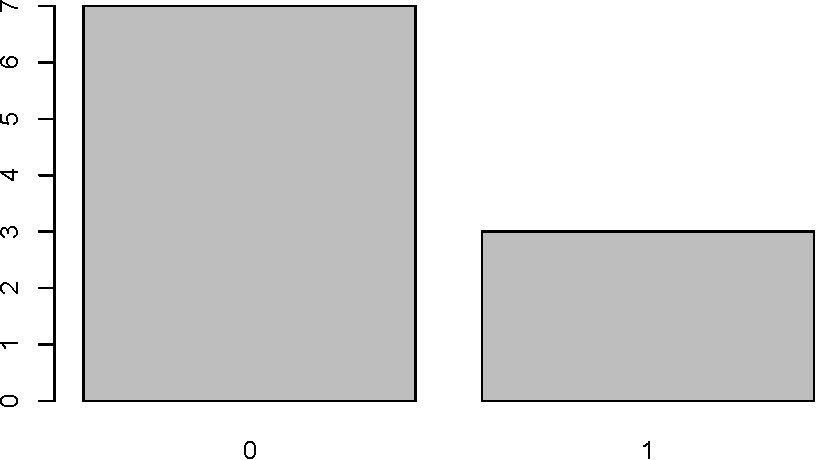
\includegraphics[width=0.9\linewidth]{bookdown_files/figure-latex/coinToss-1} \caption{Summary bar plot of coin tosses.}\label{fig:coinToss}
\end{figure}

Running these lines of code in a script window causes this plot to appear automatically under the Plots tab in the lower right RStudio window. We can save the plot image or copy and paste it into a report using menu option Export under the Plots tab. Examining the plot shows the unusual result of seven ``tails'' and three ``heads''. We would expect the counts to be about equal for the two categories, given the assumed probability of success (p) for a fair coin of 0.5.

Can you think of a physical process (hands-on method) that would produce Bernoulli data using other values for p, such as 0.25 or 0.33? What value for p might you expect for a fisheries examples, such as an annual exploitation rate (probability of being harvested), tag reporting rate (probability of angler returning a tag), or survival rate of adult fish in a lake (probability of surviving from year i to i+1)? These are the kinds of parameters that a field biologist might need to estimate. In the chapters that follow, we will examine some methods for collecting the data and estimating those probabilities.

We can generate simulated observations from a Bernoulli distribution using the \texttt{rbinom()} function:

\begin{Shaded}
\begin{Highlighting}[]
\NormalTok{N.obs }\OtherTok{\textless{}{-}} \DecValTok{30}
\NormalTok{p }\OtherTok{\textless{}{-}} \FloatTok{0.4}
\NormalTok{y }\OtherTok{\textless{}{-}} \FunctionTok{rbinom}\NormalTok{(}\AttributeTok{n=}\NormalTok{N.obs, }\AttributeTok{prob=}\NormalTok{p, }\AttributeTok{size=}\DecValTok{1}\NormalTok{)}
\NormalTok{Counts }\OtherTok{\textless{}{-}} \FunctionTok{table}\NormalTok{(y)  }\CommentTok{\# Summary table of 0 vs 1}
\FunctionTok{barplot}\NormalTok{(Counts)}
\end{Highlighting}
\end{Shaded}

The \texttt{rbinom()} function generates values from a binomial distribution (described in Section \ref{BinomialDist}). If we set the trial size to 1 (e.g., a single coin toss), we simulate draws from a Bernoulli distribution. The other two arguments in the \texttt{rbinom()} function are how many Bernoulli trials to simulate (n) and the probability of success (prob). How many values of 1 would you expect the vector y to contain in a vector of 30 replicate observations? As above, the final two lines can be used to count 0s and 1s and view a plot for these simulated data.

One of the most important benefits of using simulation is the ability to examine results from large sample sizes. For example, the following code shows that the \texttt{rbinom()} function produces an outcome very close to the expected proportion of 0s and 1s:

\begin{Shaded}
\begin{Highlighting}[]
\FunctionTok{rm}\NormalTok{(}\AttributeTok{list=}\FunctionTok{ls}\NormalTok{()) }\CommentTok{\# Clear Environment}

\NormalTok{N.obs }\OtherTok{\textless{}{-}} \DecValTok{1000}
\NormalTok{p }\OtherTok{\textless{}{-}} \FloatTok{0.4}
\NormalTok{y }\OtherTok{\textless{}{-}} \FunctionTok{rbinom}\NormalTok{(}\AttributeTok{n=}\NormalTok{N.obs, }\AttributeTok{prob=}\NormalTok{p, }\AttributeTok{size=}\DecValTok{1}\NormalTok{)}
\NormalTok{SumOnes }\OtherTok{\textless{}{-}} \FunctionTok{sum}\NormalTok{(y)}
\NormalTok{SumOnes}
\NormalTok{SumOnes}\SpecialCharTok{/}\NormalTok{N.obs }\CommentTok{\# Proportion of trials that are successful}
\NormalTok{Counts }\OtherTok{\textless{}{-}} \FunctionTok{table}\NormalTok{(y)}
\FunctionTok{barplot}\NormalTok{(Counts)}
\end{Highlighting}
\end{Shaded}

The first line of code just clears the Environment, ensuring that we start from a clean slate. The \texttt{sum()} function provides a total for the y vector, which is equal to the number of successful trials. Dividing by the number of observations is an empirical estimate of p.~The plot (Plot window) shows the result for one simulation (with N.obs replicates). How close to the expected count of 1s (400) did you observe? How much does the result vary when you do multiple simulations? (Highlight all the statements and click Run several times to see the variation.)

\hypertarget{BinomialDist}{%
\subsection{Binomial}\label{BinomialDist}}

The binomial distribution\index{Distribution, Binomial} is simply the combined total from multiple Bernoulli trials. One physical example would be the number of heads in five tosses of a coin. Each toss is an independent Bernoulli trial, but we record the total number of successes (heads). We could obtain anything between 0 and 5 heads in a single trial. We assume that the probability of success (p) is constant for each Bernoulli trial (e.g., each coin toss).

One fisheries example of a binomially distributed process would be the number of recaptures in a two-sample mark-recapture study. In that case, the number of fish in the second sample is the size of the trial, and fraction of the population that is marked is the probability p.~Another fisheries example would be the number of tag returns in a study to estimate the exploitation rate (rate of harvest). The number of tagged fish is the size of the trial and the exploitation rate is p.~A telemetry study to estimate fish survival rate is a third example. The initial number of fish with transmitters is the size of the trial. The survival rate is p and the number of survivors at the start of the next period is binomially distributed.

Let's start with a physical example of drawing five playing cards (with replacement) and recording the number of clubs. The probability of success in this case (drawing a club) is 0.25 and there are six possible outcomes (0-5 clubs). The expected number of clubs is 1.25 (trial size * p).

\begin{Shaded}
\begin{Highlighting}[]
\FunctionTok{rm}\NormalTok{(}\AttributeTok{list=}\FunctionTok{ls}\NormalTok{()) }\CommentTok{\# Clear Environment}

\NormalTok{Clubs }\OtherTok{\textless{}{-}}\FunctionTok{c}\NormalTok{(}\DecValTok{0}\NormalTok{, }\DecValTok{0}\NormalTok{, }\DecValTok{3}\NormalTok{, }\DecValTok{3}\NormalTok{, }\DecValTok{1}\NormalTok{, }\DecValTok{1}\NormalTok{)  }\CommentTok{\# Drawing five cards, with replacement}
\NormalTok{N.trials }\OtherTok{\textless{}{-}} \FunctionTok{length}\NormalTok{(Clubs) }\CommentTok{\# Function for getting number of trials}
\NormalTok{Counts }\OtherTok{\textless{}{-}} \FunctionTok{table}\NormalTok{(Clubs)}
\FunctionTok{barplot}\NormalTok{(Counts)}
\FunctionTok{barplot}\NormalTok{(Counts, }\AttributeTok{xlab=}\StringTok{"Number of clubs"}\NormalTok{)}
\end{Highlighting}
\end{Shaded}

Again we let R count the number of trials (6 in this case) and use the \texttt{table()} function to summarize the outcomes. Our sample size is small and the plot only shows the three observed outcomes. The plot can be made more understandable (especially by someone else) by adding a plot option (xlab) to label the x axis. Doing more than one plot produces a sequence of plots which you can view by using the blue left and right arrows in the Plot window. Practice modifying the above code by adding a label for the y axis (e.g., ``Frequency''). You can find the full list of bar plot options by entering ``barplot'' in the search box in the RStudio help window (or simply type ?barplot) in the Console).

We can alleviate our small sample size issue by turning to a simulation version. We again use the \texttt{rbinom()} function from the Bernoulli example, but now size is greater than 1:

\begin{Shaded}
\begin{Highlighting}[]
\FunctionTok{rm}\NormalTok{(}\AttributeTok{list=}\FunctionTok{ls}\NormalTok{()) }\CommentTok{\# Clear Environment}

\NormalTok{N.trials }\OtherTok{\textless{}{-}} \DecValTok{30}
\NormalTok{p }\OtherTok{\textless{}{-}} \FloatTok{0.25} \CommentTok{\# Probability of drawing a club}
\NormalTok{Trial.size }\OtherTok{\textless{}{-}} \DecValTok{5}
\NormalTok{Clubs }\OtherTok{\textless{}{-}} \FunctionTok{rbinom}\NormalTok{(}\AttributeTok{n=}\NormalTok{N.trials, }\AttributeTok{prob=}\NormalTok{p, }\AttributeTok{size=}\NormalTok{Trial.size)}
\NormalTok{Clubs}
\NormalTok{Counts }\OtherTok{\textless{}{-}} \FunctionTok{table}\NormalTok{(Clubs)}
\FunctionTok{barplot}\NormalTok{(Counts)}
\end{Highlighting}
\end{Shaded}

Each of the thirty observations now represents a trial size of 5 (in total, a simulation equivalent to 150 Bernoulli trials). Only part of the Clubs vector is visible in the Environment window but we can put Clubs as a line of code to print the whole vector in the Console. We again summarize the counts and plot the results using the \texttt{barplot()} function. Highlight the code in the Source window and run it multiple times to get some insight into the variability of the simulated system. For example, how often do you observe 0 or 5 Clubs? Which outcome(s) occurs most often (mode) and how frequently does the mode change?

We would expect to observe very few trials with 5 successes, because the probability is quite low (0.25\textsuperscript{5}=0.001). We can calculate it in the Console, by entering the expression 0.25\^{}5. There is a higher probability of 0 successes (0.24), which can be calculated as 0.75\^{}5 or (1-p)\textsuperscript{5}, because 1-p is the probability of failure (not getting a club). It is more involved to calculate the probabilities of 1-4 successes because they can be obtained multiple ways (e.g., 1 success can be obtained five ways (10000, 01000, 00100, 00010, 00001). We could calculate those probabilities using the binomial probability distribution: \(f(k) = {n \choose k} p^{k} (1-p)^{n-k}\), where k is the number of successes in a trial of size n.~R code for this calculation uses the \texttt{choose()} function; for example, \texttt{choose(Trial.size,0)\ *\ p\^{}0\ *\ (1-p)\^{}5} calculates the probability of 0 clubs in five draws. We could get an approximate (``brute force'') estimate of the probabilities by increasing N.trials to a large value (say 10,000) and dividing the Counts vector by N.trials to estimate at the proportion of trials resulting in 0, 1,\ldots5 successes:

\begin{Shaded}
\begin{Highlighting}[]
\FunctionTok{rm}\NormalTok{(}\AttributeTok{list=}\FunctionTok{ls}\NormalTok{()) }\CommentTok{\# Clear Environment}

\NormalTok{N.trials }\OtherTok{\textless{}{-}} \DecValTok{10000}
\NormalTok{p }\OtherTok{\textless{}{-}} \FloatTok{0.25} \CommentTok{\# Probability of drawing a club}
\NormalTok{Trial.size }\OtherTok{\textless{}{-}} \DecValTok{5}
\NormalTok{Clubs }\OtherTok{\textless{}{-}} \FunctionTok{rbinom}\NormalTok{(}\AttributeTok{n=}\NormalTok{N.trials, }\AttributeTok{prob=}\NormalTok{p, }\AttributeTok{size=}\NormalTok{Trial.size)}
\CommentTok{\#Clubs}
\NormalTok{Counts }\OtherTok{\textless{}{-}} \FunctionTok{table}\NormalTok{(Clubs)}
\FunctionTok{barplot}\NormalTok{(Counts)}
\NormalTok{Counts}\SpecialCharTok{/}\NormalTok{N.trials }\CommentTok{\# Vector division {-} probabilities of 0{-}5 Clubs}
\end{Highlighting}
\end{Shaded}

Note that we used a pound sign to turn off (``comment out'') the line for printing the Clubs vector to the Console, and print to the Console the estimated probabilities. The mode of our simulated distribution is in agreement with the expected value (trial size * p), as are the estimated probabilities for 0 and 5 clubs.

\hypertarget{Multinomial}{%
\subsection{Multinomial}\label{Multinomial}}

The Bernoulli and binomial distributions return a single value: success or failure for the Bernoulli and the number of successes (out of a specified trial size) for the binomial. The multinomial distribution\index{Distribution, Multinomial} extends that to a vector of results. A classic physical example would be to roll a die several times and record how many rolls were a 1, 2, \ldots, 6. A fisheries example would be to collect a sample of fish and determine how many are age 1, 2,\ldots{} The focus in that example is on estimating the age distribution, or proportions of fish by age. An age distribution contains valuable information about the rates of mortality and recruitment (year-class strength). Another fisheries example would be to collect a sample of fish (e.g., from electrofishing or a trawl) and determine the number caught by species. Species composition can be an important indicator of the ecological health of a study site (e.g.~if there is a high relative abundance of species considered tolerant of poor water quality).

Let's begin with a hands-on example. I roll a die ten times, and record as a vector the number of times I get a 1, 2, \ldots, 6:

\begin{Shaded}
\begin{Highlighting}[]
\FunctionTok{rm}\NormalTok{(}\AttributeTok{list=}\FunctionTok{ls}\NormalTok{()) }\CommentTok{\# Clear Environment}

\NormalTok{x }\OtherTok{\textless{}{-}}\FunctionTok{c}\NormalTok{(}\DecValTok{2}\NormalTok{,}\DecValTok{3}\NormalTok{,}\DecValTok{3}\NormalTok{,}\DecValTok{0}\NormalTok{,}\DecValTok{2}\NormalTok{,}\DecValTok{0}\NormalTok{)  }\CommentTok{\# Generated using die, equal cell probabilities}
\NormalTok{SampleSize }\OtherTok{\textless{}{-}} \FunctionTok{sum}\NormalTok{(x)}
\FunctionTok{barplot}\NormalTok{(x)}
\end{Highlighting}
\end{Shaded}

Here R calculates the sample size (SampleSize), even though we know in this instance that there were 10 rolls. The \texttt{barplot()} function generates the plot but without any labels is not very appealing. We can dress it up a bit by adding some options (Figure \ref{fig:dieRoll}). We first create a vector with values 1-6 to serve as x-axis labels (\texttt{seq()} function, from 1 to 6 by 1). Then we use the names.arg option to add the labels, and add x and y axis titles using xlab and ylab respectively.

\begin{Shaded}
\begin{Highlighting}[]
\NormalTok{x.labels }\OtherTok{\textless{}{-}} \FunctionTok{seq}\NormalTok{(}\AttributeTok{from=}\DecValTok{1}\NormalTok{, }\AttributeTok{to=}\DecValTok{6}\NormalTok{, }\AttributeTok{by=}\DecValTok{1}\NormalTok{)  }\CommentTok{\# x axis labels for plotting}
\FunctionTok{barplot}\NormalTok{(x, }\AttributeTok{names.arg=}\NormalTok{x.labels, }\AttributeTok{xlab=}\StringTok{"Die side"}\NormalTok{, }\AttributeTok{ylab=}\StringTok{"Number of rolls"}\NormalTok{)}
\end{Highlighting}
\end{Shaded}

\begin{figure}
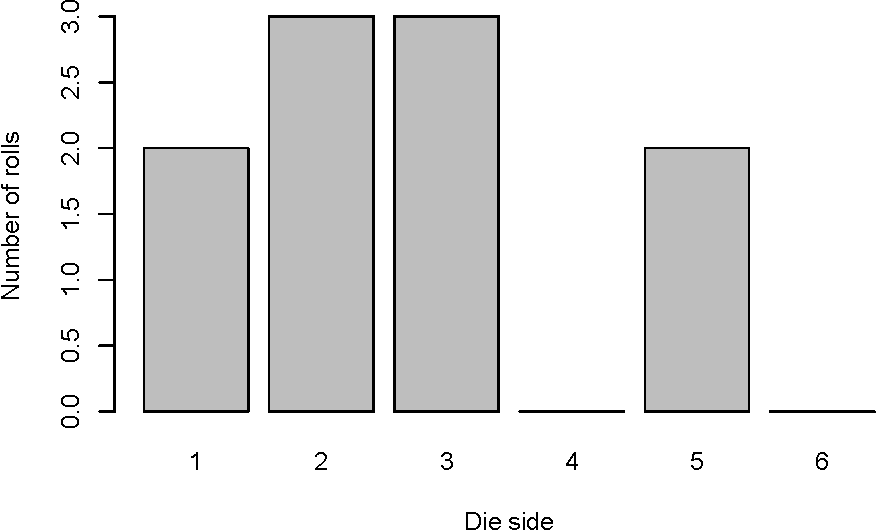
\includegraphics[width=0.9\linewidth]{bookdown_files/figure-latex/dieRoll-1} \caption{Summary bar plot of die rolls.}\label{fig:dieRoll}
\end{figure}

We can simulate a multinomial distribution as follows:

\begin{Shaded}
\begin{Highlighting}[]
\FunctionTok{rm}\NormalTok{(}\AttributeTok{list=}\FunctionTok{ls}\NormalTok{()) }\CommentTok{\# Clear Environment}

\NormalTok{SampleSize }\OtherTok{\textless{}{-}} \DecValTok{30}  \CommentTok{\# e.g., sample of 30 fish assigned by age}
\NormalTok{TrueP }\OtherTok{\textless{}{-}} \FunctionTok{c}\NormalTok{(}\FloatTok{0.1}\NormalTok{, }\FloatTok{0.3}\NormalTok{, }\FloatTok{0.4}\NormalTok{, }\FloatTok{0.1}\NormalTok{, }\FloatTok{0.05}\NormalTok{, }\FloatTok{0.05}\NormalTok{) }\CommentTok{\# probability of being ages 1{-}6}
\NormalTok{Reps }\OtherTok{\textless{}{-}} \DecValTok{1} \CommentTok{\# How many replicate multinomial trials to carry out}

\CommentTok{\# Simulate a single trial using rmultinom function}
\FunctionTok{rmultinom}\NormalTok{(}\AttributeTok{n=}\NormalTok{Reps, }\AttributeTok{prob=}\NormalTok{TrueP, }\AttributeTok{size=}\NormalTok{SampleSize) }\CommentTok{\# Prints matrix to Console}
\NormalTok{x }\OtherTok{\textless{}{-}} \FunctionTok{rmultinom}\NormalTok{(}\AttributeTok{n=}\NormalTok{Reps, }\AttributeTok{prob=}\NormalTok{TrueP, }\AttributeTok{size=}\NormalTok{SampleSize)}
\CommentTok{\# x contains matrix of counts (one column per Rep)}
\NormalTok{x.vec }\OtherTok{\textless{}{-}} \FunctionTok{as.vector}\NormalTok{(}\FunctionTok{t}\NormalTok{(x)) }\CommentTok{\# Transpose matrix then convert to vector}

\NormalTok{age.vec }\OtherTok{\textless{}{-}} \FunctionTok{seq}\NormalTok{(}\DecValTok{1}\NormalTok{,}\DecValTok{6}\NormalTok{, }\AttributeTok{by=}\DecValTok{1}\NormalTok{)}
\FunctionTok{barplot}\NormalTok{(x.vec, }\AttributeTok{names.arg=}\NormalTok{age.vec, }\AttributeTok{xlab=}\StringTok{"Age"}\NormalTok{, }\AttributeTok{ylab=}\StringTok{"Number of fish"}\NormalTok{)}
\end{Highlighting}
\end{Shaded}

In this simulation, the age proportions (TrueP) are arbitrarily chosen (but could be based on field data). Run statements one-by-one to see how each line of code works. Note that the \texttt{rmultinom()} function returns a matrix with six rows and one column (n determines how many columns are returned). Rather than a column, we want a row vector, with the number of fish by age in successive columns. We use the \texttt{t()} (transpose) function to transpose the matrix and the \texttt{as.vector()} function to convert the matrix (with one row) into a row vector. We could have done this transformation in two steps but instead have nested the two functions. That results in more compact code but it is always a fine option to do the steps separately for greater clarity.

Run the code beginning with the \texttt{x\ \textless{}-\ rmultinom()} line several times to see how much the age distribution varies from one random sample to the next. The underlying age proportions are fixed, but the counts vary quite a bit for this small sample size. This is an example of how simulation is helpful in gaining experience and intuition in judging pure sampling variation versus a real biological result (e.g.~good or bad year-class strength).

\hypertarget{poisson}{%
\subsection{Poisson}\label{poisson}}

Like the Bernoulli, binomial, and multinomial distributions, the Poisson\index{Distribution, Poisson} and negative binomial distributions are used for counts (non-negative whole numbers). The first three cases have an upper bound (1 for the Bernoulli, trial size for the next two) whereas the Poisson and negative binomial distributions do not (in theory, if not in practical terms). The Poisson is simpler than the negative binomial in that it is described by a single parameter, usually \(\lambda\), which represents the mean and variance of the distribution. A fisheries example of a Poisson distribution could be the number of fish per day moving upstream via a fish ladder. A model for this process could be useful for designing new fish ladders to have an appropriate capacity. Another example could be the number of fish caught per trawl tow. In this case, emphasis might be placed on how trawl catches vary from year to year, as an indication of population status.

Our simulation uses an arbitrary value for \(\lambda\):

\begin{Shaded}
\begin{Highlighting}[]
\FunctionTok{rm}\NormalTok{(}\AttributeTok{list=}\FunctionTok{ls}\NormalTok{()) }\CommentTok{\# Clear Environment}

\NormalTok{N }\OtherTok{\textless{}{-}} \DecValTok{30}
\NormalTok{lambda }\OtherTok{\textless{}{-}} \DecValTok{4}
\NormalTok{Count }\OtherTok{\textless{}{-}} \FunctionTok{rpois}\NormalTok{(}\AttributeTok{n=}\NormalTok{N, }\AttributeTok{lambda=}\NormalTok{lambda)}
\NormalTok{Freq }\OtherTok{\textless{}{-}} \FunctionTok{table}\NormalTok{(Count)  }\CommentTok{\# Distribution of simulated counts}
\FunctionTok{barplot}\NormalTok{(Freq, }\AttributeTok{main=}\StringTok{""}\NormalTok{, }\AttributeTok{xlab=}\StringTok{"Count"}\NormalTok{, }\AttributeTok{ylab=}\StringTok{"Frequency"}\NormalTok{)}

\FunctionTok{mean}\NormalTok{(Count)}
\FunctionTok{var}\NormalTok{(Count)}
\end{Highlighting}
\end{Shaded}

Run the lines of code multiple times to gain experience with the Poisson distribution. How often is the mode of the distribution equal to \(\lambda\)? Are the estimated mean and variance (printed to the Console) close to \(\lambda\)? Increase the sample size to get a smooth distribution and reliable estimates of the two sample statistics.

It is also useful to run the code using other values for \(\lambda\). What value for \(\lambda\) causes the mode to shift to 0? At what value does the sample distribution look like a bell curve (i.e., symmetrical)? One of the key benefits of simulation is that we can easily try different scenarios to build understanding about the system being modeled.

The plot can sometimes be misleading because it only includes observed levels. We can modify the code to include levels with a frequency of zero:

\begin{Shaded}
\begin{Highlighting}[]
\FunctionTok{rm}\NormalTok{(}\AttributeTok{list=}\FunctionTok{ls}\NormalTok{()) }\CommentTok{\# Clear Environment}

\NormalTok{N }\OtherTok{\textless{}{-}} \DecValTok{30}
\NormalTok{lambda }\OtherTok{\textless{}{-}} \DecValTok{4}
\NormalTok{Count }\OtherTok{\textless{}{-}} \FunctionTok{rpois}\NormalTok{(}\AttributeTok{n=}\NormalTok{N, }\AttributeTok{lambda=}\NormalTok{lambda) }\CommentTok{\# Counts drawn from Poisson distribution}
\NormalTok{Freq }\OtherTok{\textless{}{-}} \FunctionTok{table}\NormalTok{(}\FunctionTok{factor}\NormalTok{(Count, }\AttributeTok{levels =} \DecValTok{0}\SpecialCharTok{:}\FunctionTok{max}\NormalTok{(Count)))}
\FunctionTok{barplot}\NormalTok{(Freq, }\AttributeTok{main=}\StringTok{""}\NormalTok{, }\AttributeTok{xlab=}\StringTok{"Count"}\NormalTok{, }\AttributeTok{ylab=}\StringTok{"Frequency"}\NormalTok{)}

\FunctionTok{mean}\NormalTok{(Count)}
\FunctionTok{var}\NormalTok{(Count)}
\end{Highlighting}
\end{Shaded}

Now the \texttt{table()} function operates on counts transformed into factors (categories or levels) by the \texttt{factor()} function. The levels= argument forces \texttt{factor()} to use a range of levels from 0 to \texttt{max(Count)}, in order to include levels with a frequency of zero. Try the following partial code in the Console to see the levels (``0'', ``1'', etc) created by the \texttt{factor()} function: \texttt{myfact\ \textless{}-\ factor(Count,\ levels\ =\ 0:max(Count))}.

\hypertarget{negative-binomial}{%
\subsection{Negative binomial}\label{negative-binomial}}

As noted above, the negative binomial\index{Distribution, Negative Binomial} distribution is used in similar situations to the Poisson except that it has two parameters and is therefore more flexible. This is particularly helpful for ecological data, where counts are often more variable than would be expected under a Poisson distribution \citep{bolker2008, link.barker_2009}. The R function for generating negative binomial random variates (\texttt{rnbinom()}) can be parameterized in different ways; we use the ``ecological'' parameterization recommended by \citet{bolker2008}. This uses the mean (termed \(\mu\)) but not the variance, instead using an overdispersion parameter k. Lower values of k result in a more heterogeneous distribution, and in ecological settings, k is often less than the mean \citep{bolker2008}. The distribution approximates a Poisson when k is large. The code includes calculation of the variance as a function of mu and k \citep{bolker2008}. Alternatively the mean and variance (V) can be specified and used to solve for k: \(k = \mu^2/(V-\mu)\).

\begin{Shaded}
\begin{Highlighting}[]
\FunctionTok{rm}\NormalTok{(}\AttributeTok{list=}\FunctionTok{ls}\NormalTok{()) }\CommentTok{\# Clear Environment}

\NormalTok{N }\OtherTok{\textless{}{-}} \DecValTok{30}
\NormalTok{mu }\OtherTok{\textless{}{-}} \DecValTok{4}
\NormalTok{k}\OtherTok{=}\DecValTok{1}
\NormalTok{variance }\OtherTok{\textless{}{-}}\NormalTok{ mu}\SpecialCharTok{+}\NormalTok{(mu}\SpecialCharTok{\^{}}\DecValTok{2}\NormalTok{)}\SpecialCharTok{/}\NormalTok{k}
\NormalTok{Count }\OtherTok{\textless{}{-}} \FunctionTok{rnbinom}\NormalTok{(}\AttributeTok{n=}\NormalTok{N, }\AttributeTok{mu=}\NormalTok{mu, }\AttributeTok{size=}\NormalTok{k)}
\NormalTok{Freq }\OtherTok{\textless{}{-}} \FunctionTok{table}\NormalTok{(}\FunctionTok{factor}\NormalTok{(Count, }\AttributeTok{levels =} \DecValTok{0}\SpecialCharTok{:}\FunctionTok{max}\NormalTok{(Count)))}
\FunctionTok{barplot}\NormalTok{(Freq, }\AttributeTok{main=}\StringTok{""}\NormalTok{, }\AttributeTok{xlab=}\StringTok{"Count"}\NormalTok{, }\AttributeTok{ylab=}\StringTok{"Frequency"}\NormalTok{)}

\FunctionTok{mean}\NormalTok{(Count)}
\FunctionTok{var}\NormalTok{(Count)}
\end{Highlighting}
\end{Shaded}

This distribution has the same mean as in the Poisson example but tends to have a longer tail (occasional large counts). Rerun the code using different values for k; for example, Figure \ref{fig:NB-vary-k} uses a sample size of 200 to compare results for k=1 and k=10, each with \(\mu\)=4.

\begin{Shaded}
\begin{Highlighting}[]
\NormalTok{N }\OtherTok{\textless{}{-}} \DecValTok{200}
\NormalTok{mu }\OtherTok{\textless{}{-}} \DecValTok{4}
\NormalTok{k}\OtherTok{=}\DecValTok{1}
\NormalTok{Count }\OtherTok{\textless{}{-}} \FunctionTok{rnbinom}\NormalTok{(}\AttributeTok{n=}\NormalTok{N, }\AttributeTok{mu=}\NormalTok{mu, }\AttributeTok{size=}\NormalTok{k)}
\NormalTok{Freq }\OtherTok{\textless{}{-}} \FunctionTok{table}\NormalTok{(}\FunctionTok{factor}\NormalTok{(Count, }\AttributeTok{levels =} \DecValTok{0}\SpecialCharTok{:}\FunctionTok{max}\NormalTok{(Count)))}
\FunctionTok{barplot}\NormalTok{(Freq, }\AttributeTok{main=}\StringTok{""}\NormalTok{, }\AttributeTok{xlab=}\StringTok{"Count"}\NormalTok{, }\AttributeTok{ylab=}\StringTok{"Frequency"}\NormalTok{)}

\NormalTok{k}\OtherTok{=}\DecValTok{10} \CommentTok{\# Reduce degree of overdispersion}
\NormalTok{Count }\OtherTok{\textless{}{-}} \FunctionTok{rnbinom}\NormalTok{(}\AttributeTok{n=}\NormalTok{N, }\AttributeTok{mu=}\NormalTok{mu, }\AttributeTok{size=}\NormalTok{k)}
\NormalTok{Freq }\OtherTok{\textless{}{-}} \FunctionTok{table}\NormalTok{(}\FunctionTok{factor}\NormalTok{(Count, }\AttributeTok{levels =} \DecValTok{0}\SpecialCharTok{:}\FunctionTok{max}\NormalTok{(Count)))}
\FunctionTok{barplot}\NormalTok{(Freq, }\AttributeTok{main=}\StringTok{""}\NormalTok{, }\AttributeTok{xlab=}\StringTok{"Count"}\NormalTok{, }\AttributeTok{ylab=}\StringTok{"Frequency"}\NormalTok{)}
\end{Highlighting}
\end{Shaded}

\begin{figure}
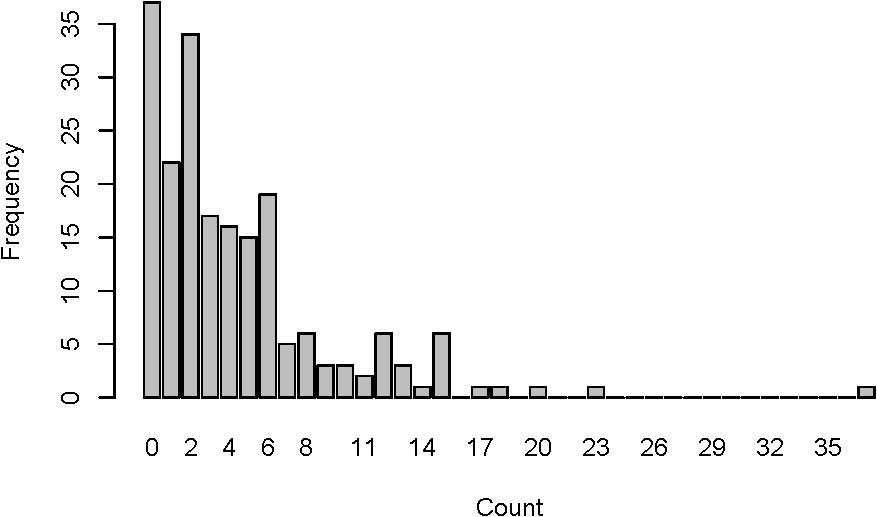
\includegraphics[width=0.5\linewidth]{bookdown_files/figure-latex/NB-vary-k-1} 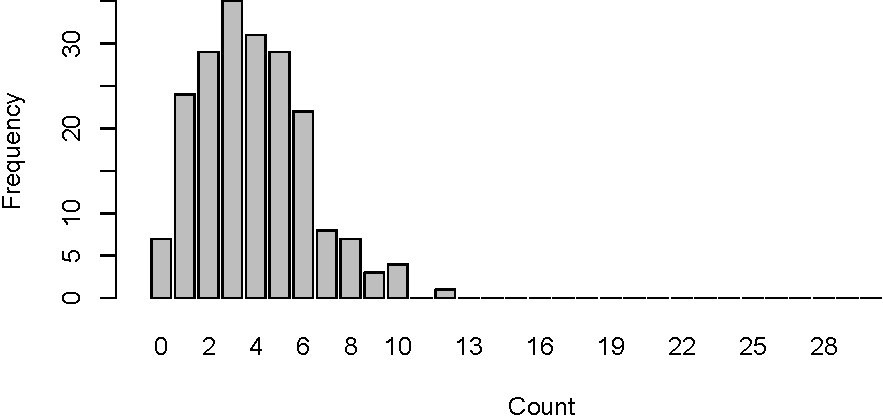
\includegraphics[width=0.5\linewidth]{bookdown_files/figure-latex/NB-vary-k-2} \caption{Negative binomial frequency distributions for k=1 (left) and 10 (right).}\label{fig:NB-vary-k}
\end{figure}

\hypertarget{Continuous}{%
\section{Continuous}\label{Continuous}}

\hypertarget{Uniform}{%
\subsection{Uniform}\label{Uniform}}

A uniform distribution\index{Distribution, Uniform} (bounds a, b) is flat in shape, indicating that all values between a lower and upper bound are considered equally likely. It is also useful as a ``first'' model for situations where relatively little is known other than the lower and upper bounds \citep{law.kelton_1982}. Probabilities have default bounds of 0 and 1, so a fish population model might use a uniform 0-1 distribution for probabilities such as survival rate. More narrow bounds could be used in cases where prior information was available; for example, a pilot study might indicate that the tag-reporting rate would be expected to vary between 0.4 and 0.6. Another fisheries example would be a uniform distribution between 60 and 70, for simulating individual variation in maximum size for a growth curve.

We begin with a simulation example, using the default range of 0-1 for the \texttt{runif()} function:

\begin{Shaded}
\begin{Highlighting}[]
\FunctionTok{rm}\NormalTok{(}\AttributeTok{list=}\FunctionTok{ls}\NormalTok{()) }\CommentTok{\# Clear Environment}

\NormalTok{Reps }\OtherTok{\textless{}{-}} \DecValTok{30} \CommentTok{\# Replicate draws from a uniform distribution}
\NormalTok{p }\OtherTok{\textless{}{-}} \FunctionTok{runif}\NormalTok{(}\AttributeTok{n=}\NormalTok{Reps)}\CommentTok{\# Default range of 0{-}1. Can specify using min, max}
\FunctionTok{hist}\NormalTok{(p, }\AttributeTok{breaks=}\DecValTok{5}\NormalTok{, }\AttributeTok{main=}\StringTok{""}\NormalTok{)}
\end{Highlighting}
\end{Shaded}

Try running the code several times and note the variation in pattern from one simulation run to the next. We use the breaks=5 option in the \texttt{hist()} function so that the histogram bin intervals are stable among runs. Specifying a null character string for ``main='' prevents the plot from including a main title. Next, increase the sample size and note the increased smoothness of the observed distribution. What would be the expected mean of the distribution? Estimate the mean and compare the observed and expected value among runs.

As noted above, the \texttt{runif()} function allows for a uniform distribution using any lower and upper bounds. For example, we might simulate uncertainty about an exploitation rate (fraction of the population that is harvested) by allowing randomly drawn values in a specified interval; for example, \texttt{runif(n=Reps,\ min=0.3,\ max=0.4)}. The \texttt{runif()} function is not constrained to positive values; for example, it could be used with bounds -0.5 and 0.5 to simulate uncertainty about a parameter that is close to 0 but can be positive or negative. The chapters that follow will include many examples where a uniform distribution is relevant for fisheries modeling.

\hypertarget{beta}{%
\subsection{Beta}\label{beta}}

The beta distribution\index{Distribution, Beta} has a lower bound of 0 and an upper bound of 1, so it is useful for modeling parameters with those bounds (i.e., probabilities). A fisheries model might use a beta distribution to simulate variation in a survival probability or the probability of a tag being returned. The uniform distribution (Section \ref{Uniform}) can also be used for probabilities, but only for the case where all values are equally likely. The beta distribution is more flexible and can not only be flat but also u-shaped, bell-shaped, or left- or right-skewed. Figure \ref{fig:Beta} shows sample distributions for shape parameters \(\alpha\)=1 and \(\beta\)=0.5, 1, and 5.

\begin{figure}
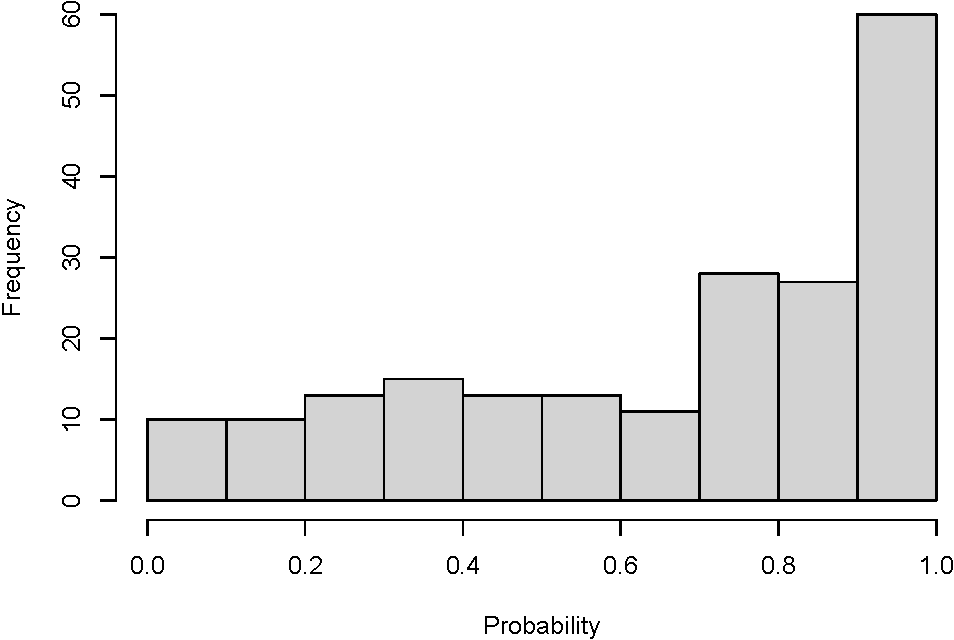
\includegraphics[width=0.33\linewidth]{bookdown_files/figure-latex/Beta-1} 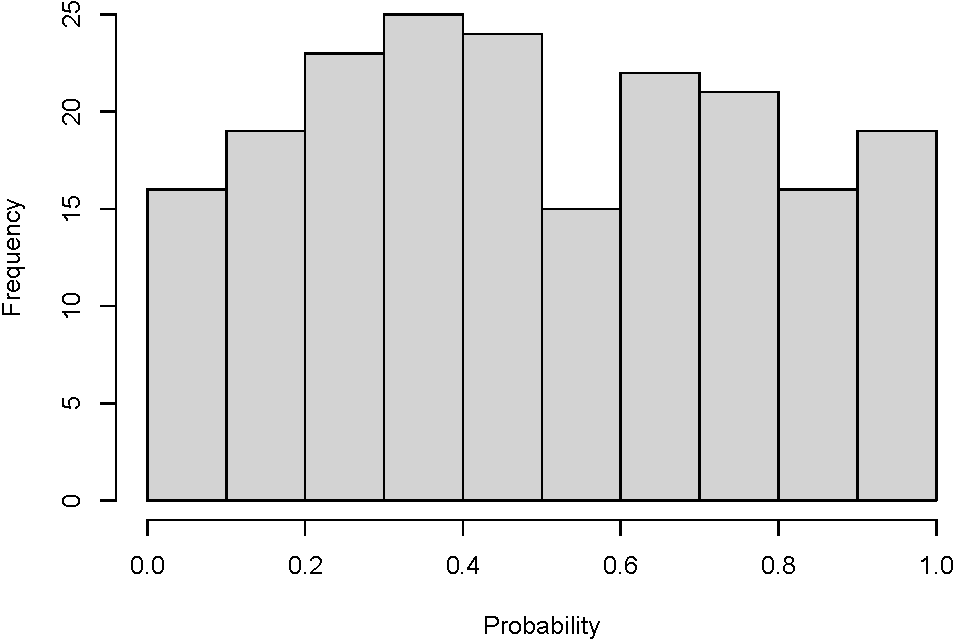
\includegraphics[width=0.33\linewidth]{bookdown_files/figure-latex/Beta-2} 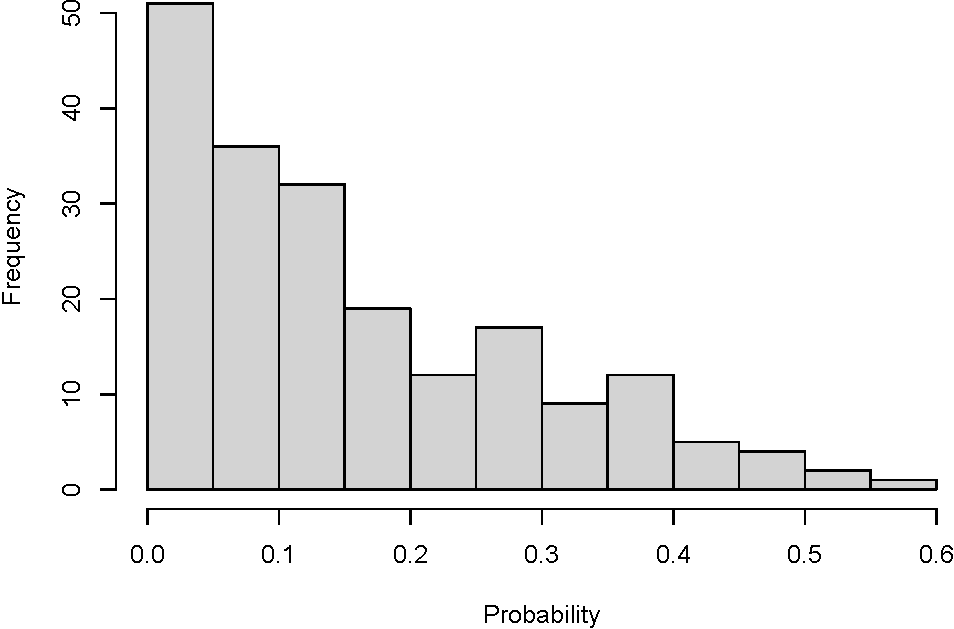
\includegraphics[width=0.33\linewidth]{bookdown_files/figure-latex/Beta-3} \caption{Histogram for 200 random draws from a beta distribution, with alpha=1 and beta=0.5  (left), 1 (center), and 5 (right).}\label{fig:Beta}
\end{figure}

We simulate draws from a beta distribution using the \texttt{rbeta()} function. Starting with \(\alpha\) and \(\beta\) set to 1 would be appropriate for a situation where all probabilities are equally likely:

\begin{Shaded}
\begin{Highlighting}[]
\FunctionTok{rm}\NormalTok{(}\AttributeTok{list=}\FunctionTok{ls}\NormalTok{()) }\CommentTok{\# Clear Environment}

\NormalTok{Reps }\OtherTok{\textless{}{-}} \DecValTok{200} \CommentTok{\# Replicate draws from a beta distribution}
\NormalTok{alpha }\OtherTok{\textless{}{-}} \DecValTok{1}
\NormalTok{beta }\OtherTok{\textless{}{-}} \DecValTok{1}
\NormalTok{x }\OtherTok{\textless{}{-}} \FunctionTok{rbeta}\NormalTok{(}\AttributeTok{n=}\NormalTok{Reps, }\AttributeTok{shape1=}\NormalTok{alpha, }\AttributeTok{shape2=}\NormalTok{beta)}
\FunctionTok{hist}\NormalTok{(x, }\AttributeTok{main=}\StringTok{""}\NormalTok{, }\AttributeTok{xlab=}\StringTok{"Probability"}\NormalTok{)}
\end{Highlighting}
\end{Shaded}

After running the above code multiple times, try a beta(8, 4) distribution. These parameter values could result from a pilot study with seven successes in ten trials (\(\alpha\)=7+1, \(\beta\)=3+1). This shifts the distribution toward a mode of 0.7, which is the observed proportion of successes in ten trials. Try other arbitrary values for the two parameters to vary the shape of the distribution. Can you think of a situation where probabilities would be expected to be close to 0 or close to 1?

\hypertarget{normal}{%
\subsection{Normal}\label{normal}}

The normal distribution\index{Distribution, Normal} is the well-known bell curve from traditional statistics courses. The distribution is unbounded (bounds -\(\infty\), \(\infty\)). The shape of the distribution is determined by the mean (location) and standard deviation (spread). A fisheries example might be a simulation where size-at-age varied among individuals according to a normal distribution.

Let's look at simulation code for length of individual fish, assuming a mean of 30 and standard deviation of 2:

\begin{Shaded}
\begin{Highlighting}[]
\FunctionTok{rm}\NormalTok{(}\AttributeTok{list=}\FunctionTok{ls}\NormalTok{()) }\CommentTok{\# Clear Environment}

\NormalTok{Reps }\OtherTok{\textless{}{-}} \DecValTok{30} \CommentTok{\# Replicate draws from a normal distribution}
\NormalTok{Len }\OtherTok{\textless{}{-}} \FunctionTok{rnorm}\NormalTok{(}\AttributeTok{n=}\NormalTok{Reps, }\AttributeTok{mean=}\DecValTok{30}\NormalTok{, }\AttributeTok{sd=}\DecValTok{2}\NormalTok{)}
\FunctionTok{hist}\NormalTok{(Len, }\AttributeTok{main=}\StringTok{""}\NormalTok{)}
\end{Highlighting}
\end{Shaded}

Run the code a few times to look at the variation in shape and bounds at a relatively small sample size. Next, increase the sample size and determine through trial and error the smallest sample size that provides a relatively smooth bell-curve shape. Estimate the mean and standard deviation (function \texttt{sd()}) and compare the observed and true values.

\hypertarget{lognormal}{%
\subsection{Lognormal}\label{lognormal}}

The lognormal distribution\index{Distribution, Lognormal} (bounds 0, \(\infty\)) is useful in ecological settings because it excludes negative values and allows for a long upper tail. A classic fisheries example of a lognormal distribution is annual recruitment for marine fish species (number of young entering the population). Most years result in low recruitment but there are occasional extreme values when environmental conditions are right.

We begin with simulation code:

\begin{Shaded}
\begin{Highlighting}[]
\FunctionTok{rm}\NormalTok{(}\AttributeTok{list=}\FunctionTok{ls}\NormalTok{()) }\CommentTok{\# Clear Environment}

\NormalTok{Reps }\OtherTok{\textless{}{-}} \DecValTok{200}
\NormalTok{ln.m }\OtherTok{\textless{}{-}} \DecValTok{0} \CommentTok{\# Ln{-}scale mean}
\NormalTok{ln.v }\OtherTok{\textless{}{-}} \FloatTok{0.5} \CommentTok{\# Ln{-}scale variance}
\NormalTok{y }\OtherTok{\textless{}{-}} \FunctionTok{rlnorm}\NormalTok{(}\AttributeTok{n=}\NormalTok{Reps, }\AttributeTok{mean=}\NormalTok{ln.m, }\AttributeTok{sd=}\FunctionTok{sqrt}\NormalTok{(ln.v))}

\FunctionTok{hist}\NormalTok{(y, }\AttributeTok{main=}\StringTok{"Lognormal distribution"}\NormalTok{)}
\NormalTok{Exp.mean }\OtherTok{\textless{}{-}} \FunctionTok{exp}\NormalTok{(ln.m}\SpecialCharTok{+}\NormalTok{(ln.v}\SpecialCharTok{/}\DecValTok{2}\NormalTok{)) }\CommentTok{\# Calculate arithmetic scale expected mean}
\FunctionTok{abline}\NormalTok{(}\AttributeTok{v=}\NormalTok{Exp.mean, }\AttributeTok{col=}\StringTok{"red"}\NormalTok{)}
\NormalTok{Exp.var }\OtherTok{\textless{}{-}}\NormalTok{ (}\FunctionTok{exp}\NormalTok{(}\DecValTok{2}\SpecialCharTok{*}\NormalTok{ln.m}\SpecialCharTok{+}\NormalTok{ln.v))}\SpecialCharTok{*}\NormalTok{(}\FunctionTok{exp}\NormalTok{(ln.v)}\SpecialCharTok{{-}}\DecValTok{1}\NormalTok{) }\CommentTok{\# Arithmetic scale expected variance}
\FunctionTok{mean}\NormalTok{(y)}
\FunctionTok{var}\NormalTok{(y)}
\end{Highlighting}
\end{Shaded}

The \texttt{rlnorm()} function generates random lognormal values, using an arbitrarily chosen mean and standard deviation specified in natural log-scale. Those values can be used to calculate the expected mean and variance in arithmetic scale. The \texttt{abline()} function can be used to add to the histogram a vertical (v=) line for the expected arithmetic-scale mean (Figure \ref{fig:Lognormal}). The line color is specified as col=``red''; other options including line weight and pattern can be found in the Help window. Compare the estimates of arithmetic-scale mean and variance for your (relatively large) sample of lognormal random variates to the expected values (visible in the Environment window).

\begin{figure}
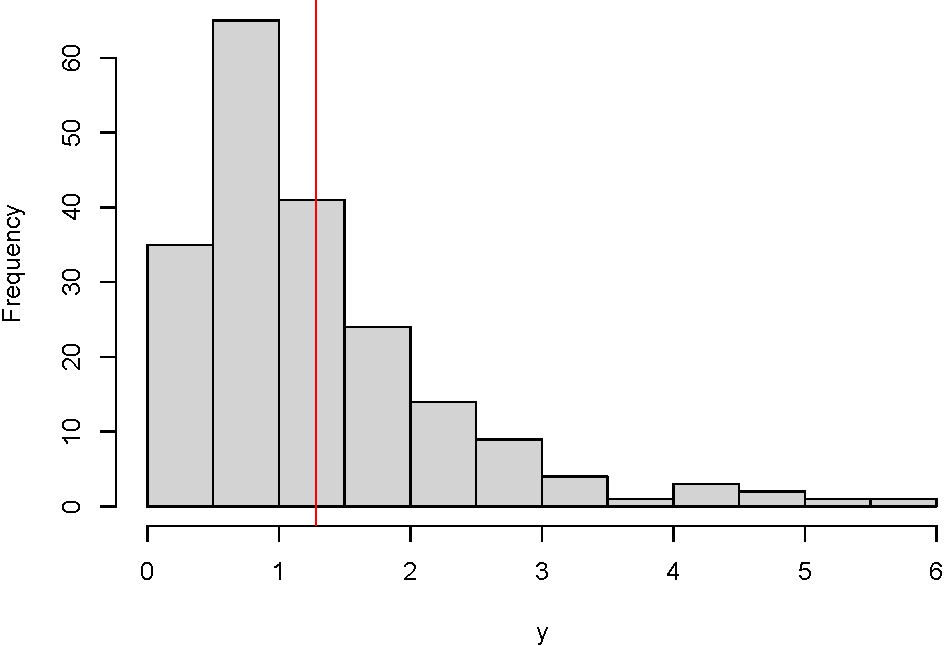
\includegraphics[width=0.9\linewidth]{bookdown_files/figure-latex/Lognormal-1} \caption{Histogram for 200 lognormally-distributed values, with ln-scale mean of 0 and variance of 0.5. Red vertical line denotes expected mean.}\label{fig:Lognormal}
\end{figure}

\hypertarget{gamma}{%
\subsection{Gamma}\label{gamma}}

The gamma distribution\index{Distribution, Gamma} is similar to the lognormal in that has a lower bound of 0 and an upper bound of \(\infty\). Thus it also excludes negative values and allows for a long upper tail. This distribution is often used to simulate waiting times (how long until some number of events has occurred, based on a specified average time between events). We consider it here simply because it can take on a variety of shapes depending on its parameters \citep{bolker2008}. Figure \ref{fig:Gamma} shows sample distributions for shape parameter \(\alpha\)=3 and scale or spread parameter \(\beta\)=1 and 3.

\begin{figure}
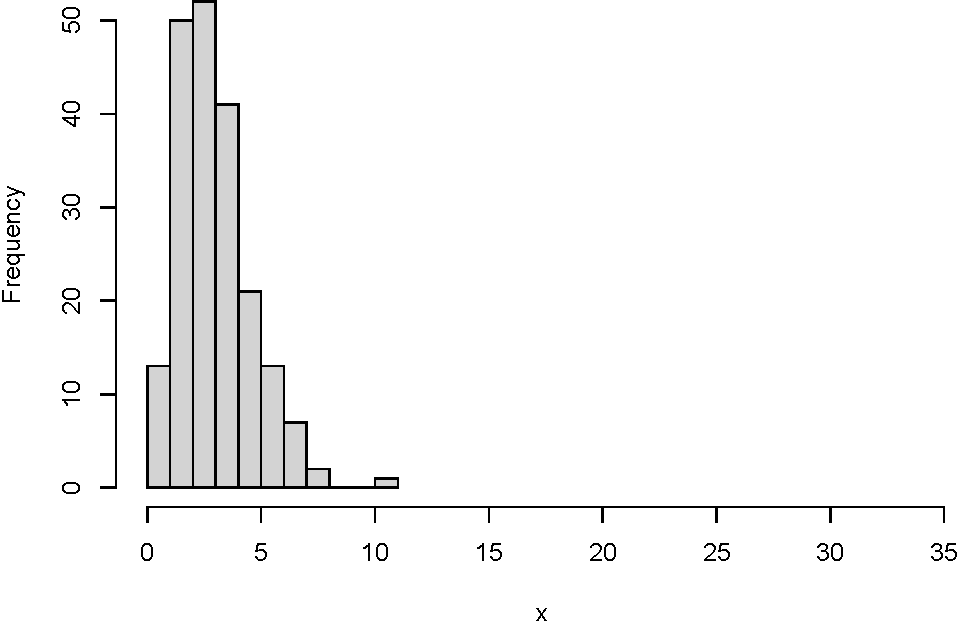
\includegraphics[width=0.5\linewidth]{bookdown_files/figure-latex/Gamma-1} 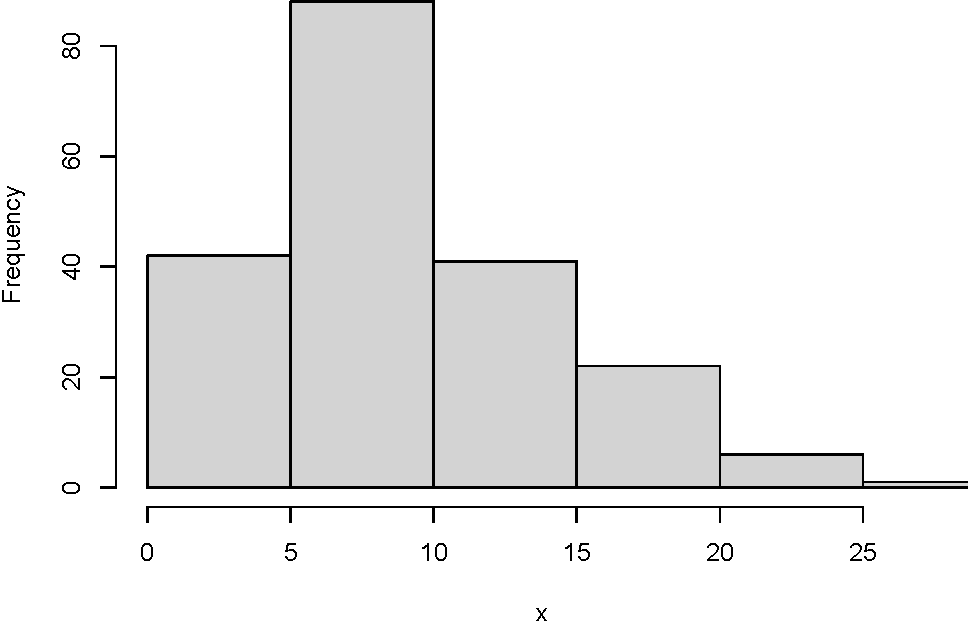
\includegraphics[width=0.5\linewidth]{bookdown_files/figure-latex/Gamma-2} \caption{Histogram for 200 gamma-distributed values, with alpha=3 and beta=1  (left) and 3 (right).}\label{fig:Gamma}
\end{figure}

We simulate draws from a gamma distribution using the \texttt{rgamma()} function, with arbitrary values for \(\alpha\) and \(\beta\):

\begin{Shaded}
\begin{Highlighting}[]
\FunctionTok{rm}\NormalTok{(}\AttributeTok{list=}\FunctionTok{ls}\NormalTok{()) }\CommentTok{\# Clear Environment}

\NormalTok{Reps }\OtherTok{\textless{}{-}} \DecValTok{200} \CommentTok{\# Replicate draws from a gamma distribution}
\NormalTok{alpha }\OtherTok{\textless{}{-}} \DecValTok{3} \CommentTok{\# Shape parameter, \textgreater{} 0}
\NormalTok{beta }\OtherTok{\textless{}{-}} \DecValTok{3} \CommentTok{\# Scale parameter, \textgreater{} 0}
\NormalTok{x }\OtherTok{\textless{}{-}} \FunctionTok{rgamma}\NormalTok{(}\AttributeTok{n=}\NormalTok{Reps, }\AttributeTok{shape=}\NormalTok{alpha, }\AttributeTok{scale=}\NormalTok{beta)}
\FunctionTok{hist}\NormalTok{(x, }\AttributeTok{main=}\StringTok{""}\NormalTok{)}
\NormalTok{Exp.mean }\OtherTok{\textless{}{-}}\NormalTok{ alpha}\SpecialCharTok{*}\NormalTok{beta}
\NormalTok{Exp.var }\OtherTok{\textless{}{-}}\NormalTok{ alpha}\SpecialCharTok{*}\NormalTok{beta}\SpecialCharTok{\^{}}\DecValTok{2}
\FunctionTok{mean}\NormalTok{(x)}
\FunctionTok{var}\NormalTok{(x)}
\end{Highlighting}
\end{Shaded}

A sample size of 200 replicates produces a relatively smooth pattern for the distribution. How close are the estimated mean and variance to the expected values for this sample size? Try adjusting the two parameters to vary the shape of the distribution. What values for \(\alpha\) and \(\beta\) produce a right-skewed distribution (long right tail), or a pattern somewhat like a normal distribution (bell-curve)?

\hypertarget{exercises}{%
\section{Exercises}\label{exercises}}

\begin{enumerate}
\def\labelenumi{\arabic{enumi}.}
\item
  Use a physical process (i.e., not simulated) to generate twenty Bernoulli observations with probability of success 0.25. Include in your code comments describing how you obtained the data. Produce a summary plot of the total number of 0s and 1s. How does your observed number of successes compare to what you would expect?
\item
  Use a physical process to generate ten binomially distributed observations, with a trial size of at least four. What is the probability of success and the expected number of successes per trial? Produce a histogram showing the frequencies for different numbers of success per trial.
\item
  Use a physical process to generate 10 outcomes from a multinomial process with at least three possible outcomes. Describe in your code comments the physical process for obtaining the data and include a plot of the frequencies. How do the frequencies compare to what you would expect?
\item
  Assume that the following vector contains trawl catches: y=c(7, 5, 1, 5, 0, 3, 8, 2, 14, 5, 0, 6, 9, 1, 2, 2, 1, 1, 0, 9, 2, 2, 4, 11, 1, 1, 7, 3, 1, 1). Based on your analysis (including plot), were these data likely generated from a Poisson or negative binomial distribution?
\item
  Provide simulation code for generating normally-distributed length data for fish ages 1 (n.1=40, age-1 mean 30, sd 5) and 2 (n.2=25, age-2 mean=50, sd=7). Plot the combined length sample. In multiple simulations using these default values, how frequently is the length distribution visibly bimodal?
\end{enumerate}

\hypertarget{Model-fit}{%
\chapter{Model Fitting}\label{Model-fit}}

\hypertarget{introduction-1}{%
\section{Introduction}\label{introduction-1}}

What is a model in a fisheries context? It typically means one or more equations that describe a biological process of interest. There are two good reasons for developing a model. A model that simulates a field study can be used for planning purposes, before field work is conducted. Such a model might be used to determine the number of fish to tag or the level of electrofishing effort, in order for the field work to produce a useful result. A model can also be used to test an analytical approach. For example, we could generate simulated data and see whether our analysis agrees with the known true value(s). The other main use of a model is to analyze data from field work. One example from Chapter \ref{R-intro} is a two-sample mark-recapture study to estimate population size. Fish in the first sample are tagged, and the fraction of marked fish in the second sample provides the information needed to estimate population size. The model in that case is the equation for population size (N\textsubscript{hat}), along with some assumptions about sampling. The equation is based on the assumption that the marked fraction of the second sample should (on average) be the same as the marked fraction in the underlying population. This method also requires some other assumptions that are more practical in nature, to help ensure that our field methods approximate the underlying model structure. For example, we assume that tagged and untagged fish are well mixed. In practice, this means that tagging effort should be well distributed throughout the study area so that our recapture effort does not encounter pockets with too many or too few tagged fish. We also assume that tags are not shed and that there are no deaths due to tagging. The mark-recapture model assumes that we know how many fish are in the tagged subpopulation. Tag loss or tagging mortality would affect that number and result in a biased estimate.

\hypertarget{Model-fit-sim}{%
\section{Using simulation}\label{Model-fit-sim}}

The equation for a two-sample mark-recapture study provides a point estimate of population size, but we could consider an improved version of the model that would allow us to more fully characterize the study results. For example, we could assume that the number of marked fish in the second sample comes from a binomial distribution. That distributional assumption allows us to generate estimates of uncertainty as well as the point estimate. The key to this sort of extended model is to think about the process generating the field data and determine which statistical distribution is appropriate. Let's start with a simulation then consider an alternative (Bayesian) approach.

\begin{Shaded}
\begin{Highlighting}[]
\FunctionTok{rm}\NormalTok{(}\AttributeTok{list=}\FunctionTok{ls}\NormalTok{()) }\CommentTok{\# Clear Environment}

\CommentTok{\# Two{-}sample population estimate}
\NormalTok{N.true }\OtherTok{\textless{}{-}} \DecValTok{400}  \CommentTok{\# Arbitrary assumed population size}
\NormalTok{p.true }\OtherTok{\textless{}{-}} \FloatTok{0.2} \CommentTok{\# Capture probability (fraction of population sampled)}
\NormalTok{n1 }\OtherTok{\textless{}{-}}\NormalTok{ N.true }\SpecialCharTok{*}\NormalTok{ p.true }\CommentTok{\# Number caught and marked in first sample}
\NormalTok{n2 }\OtherTok{\textless{}{-}}\NormalTok{ N.true }\SpecialCharTok{*}\NormalTok{ p.true }\CommentTok{\# Number caught and examined for marks in second sample}
\NormalTok{m2 }\OtherTok{\textless{}{-}}\NormalTok{ n2 }\SpecialCharTok{*}\NormalTok{ p.true }\CommentTok{\# Number of marked fish in second sample}
\NormalTok{N.hat }\OtherTok{\textless{}{-}}\NormalTok{ n1}\SpecialCharTok{*}\NormalTok{n2}\SpecialCharTok{/}\NormalTok{m2 }\CommentTok{\# Store estimate as variable N\_hat}
\end{Highlighting}
\end{Shaded}

This example uses the same estimator as in Chapter \ref{R-intro}. The two samples could be fixed values and could differ, but here we assume they are equal in size, based on the capture probability (p.true). The number of recaptures in the second sample equals the expected number based on the fraction of the population that is marked (p.true). Because n\textsubscript{1}, n\textsubscript{2}, and m\textsubscript{2} take on their expected values based on p.true, the estimate (N\textsubscript{hat}) equals the true value (see Environment window).

Now, let's extend the model by introducing some randomness (stochasticity) in the number of recaptures. We assume that recaptures are the successes in a binomial trial. The size of the binomial trial is n\textsubscript{2}. The probability of success equals p.true here but we calculate it as n\textsubscript{1}/N.true in case n\textsubscript{1} and n\textsubscript{2} were given other fixed values.

\begin{Shaded}
\begin{Highlighting}[]
\CommentTok{\# Extend model to allow for stochasticity}
\NormalTok{Reps }\OtherTok{\textless{}{-}} \DecValTok{1000}
\NormalTok{m2.vec }\OtherTok{\textless{}{-}} \FunctionTok{rbinom}\NormalTok{(}\AttributeTok{n=}\NormalTok{Reps, }\AttributeTok{prob=}\NormalTok{n1}\SpecialCharTok{/}\NormalTok{N.true, }\AttributeTok{size=}\NormalTok{n2)}
\NormalTok{N.hat }\OtherTok{\textless{}{-}}\NormalTok{ n1 }\SpecialCharTok{*}\NormalTok{ n2 }\SpecialCharTok{/}\NormalTok{ m2.vec}
\end{Highlighting}
\end{Shaded}

The rbinom() function produces a vector of recaptures, simulating a mark-recapture study repeated Reps times. Using that vector in the equation for N\textsubscript{hat} now produces a vector of population estimates. Plotting those results (Figure \ref{fig:Bootstrap}) shows that estimates are generally close to the true value but tend to have a long tail to the right (overestimates N\textsubscript{hat} when a low value is drawn for the number of recaptures).

\begin{Shaded}
\begin{Highlighting}[]
\FunctionTok{hist}\NormalTok{(m2.vec, }\AttributeTok{xlab=}\StringTok{"Number of recaptures"}\NormalTok{, }\AttributeTok{main=}\StringTok{""}\NormalTok{)}
\FunctionTok{hist}\NormalTok{(N.hat, }\AttributeTok{xlab=}\StringTok{"Population estimate"}\NormalTok{, }\AttributeTok{main=}\StringTok{""}\NormalTok{)}
\end{Highlighting}
\end{Shaded}

\begin{figure}
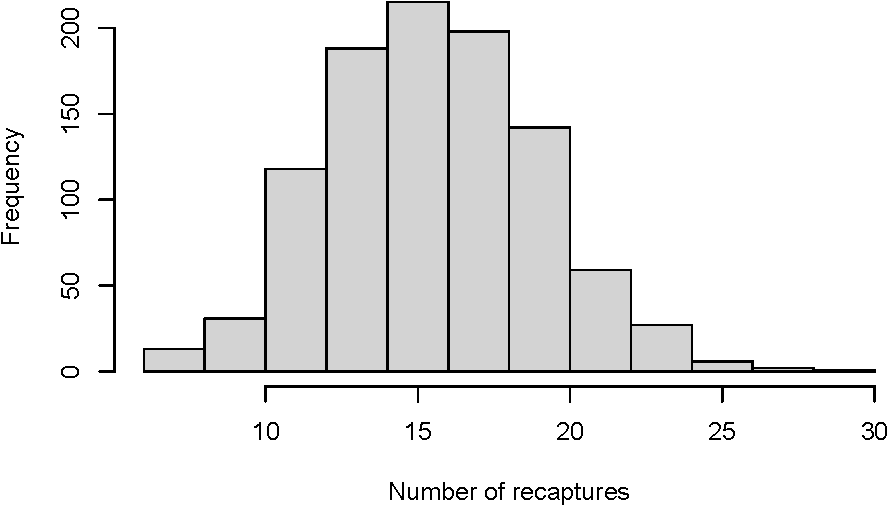
\includegraphics[width=0.5\linewidth]{bookdown_files/figure-latex/Bootstrap-1} 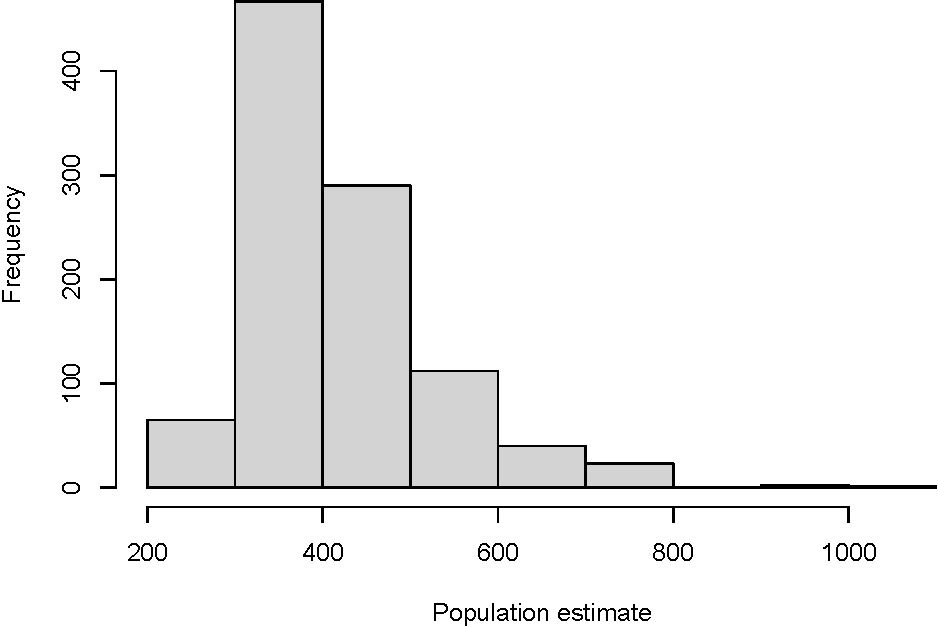
\includegraphics[width=0.5\linewidth]{bookdown_files/figure-latex/Bootstrap-2} \caption{Frequency distributions for number of recaptured fish (left) and estimated population size (right), based on simulation using a binomial distribution for the number of recaptures.}\label{fig:Bootstrap}
\end{figure}

\begin{Shaded}
\begin{Highlighting}[]
\FunctionTok{mean}\NormalTok{(N.hat)}
\FunctionTok{quantile}\NormalTok{(N.hat, }\AttributeTok{probs=}\FunctionTok{c}\NormalTok{(}\FloatTok{0.025}\NormalTok{, }\FloatTok{0.5}\NormalTok{, }\FloatTok{0.975}\NormalTok{), }\AttributeTok{na.rm=}\ConstantTok{TRUE}\NormalTok{)}
\CommentTok{\# quantile function provides empirical confidence bounds and median}
\end{Highlighting}
\end{Shaded}

Results printed to the Console show that the mean is higher than the true value (due to the tail of extreme values) but the median is very close to N.true. The estimated median and 95\% bounds are obtained using the quantile() function. We provide a vector of probabilities and the function returns the estimates at those points. The 0.025 and 0.975 points provide the empirical 95\% bounds, and the 0.5 point is the median. There are less biased modifications to the basic two-sample estimator but this version is more intuitive and sufficient for our purposes. When interpreting a field study of this sort, the confidence bounds and overall shape of the distribution should be given more emphasis than the point estimate (which reduces concern about any statistical bias of the estimator).

\hypertarget{JAGS-model-fit}{%
\section{Using Bayesian methods}\label{JAGS-model-fit}}

In Section \ref{Model-fit-sim}, we used a simulation-based or numerical approach to estimate confidence limits for the mark-recapture study design. This is an example of parametric bootstrapping \citep{efron.tibshirani_1993}, where replicate samples (number of recaptured fish in this case) are drawn from a parametric distribution, in this case binomial. We can compare this simulation approach to a formal statistical method, using a Bayesian framework. We use the same binomial distribution to describe the process of obtaining recaptures. Our results will be similar, and hopefully the comparison will provide some intuition about how a Bayesian analysis works. Our use of simulation in the remainder of the book will be limited to generating ``sample'' data. Model fitting will be done using Bayesian methods that work well for simple or complex models.

The two paradigms for statistical methods are frequentist\index{frequentist} and Bayesian\index{Bayesian}. Frequentist methods are the classical approach for estimating model parameters and making inferences \citep{royle.dorazio_2009}. In a frequentist framework, model parameters are assumed to be fixed but unknown values. For example, we could conduct a two-sample mark-recapture study to estimate population size in a lake. If we repeated the mark-recapture study many times, we would expect the 95\% confidence limit for each estimate to contain the true population size 95 percent of the time (hence the term frequentist).

A Bayesian analysis is based on the data in hand and does not rely on the idea of hypothetical replicate studies \citep{mccarthy2007, royle.dorazio_2009}. The results are exact for any sample size \citep{kéry.schaub_2011}, which is an important advantage for fisheries studies because sample sizes are often small. Bayesian statistics also differs from frequentist statistics in that it takes into account what is known before the study is conducted \citep{mccarthy2007}. The requirement to specify prior knowledge can be viewed as either an advantage or disadvantage, depending on the availability of prior data and one's statistical philosophy \citep{ellison_2004, mccarthy2007, kéry_2010, kéry.schaub_2011, dorazio_2016, doll.jacquemin_2018}. The prior information takes the form of a statistical distribution that defines the range and relative likelihood of possible values (prior to collecting the new data). The prior distribution\index{Distribution, prior} can be informative or uninformative. For example, a uniform 0-1 distribution would be a uninformative prior for a tag-reporting rate, because probabilities are by definition constrained to be between 0 and 1. Results from a pilot study might allow for an informative prior distribution; for example, a uniform distribution between 0.2 and 0.4.

\citet{lunn.etal2012} note that a substantial degree of judgement is involved in selecting relevant data for a prior distribution. A fisheries example could be whether to use growth information from a prior year when population size was higher. Another case could be whether the tag reporting rate was now be lower than when a pilot study was done because of increased angler dissatisfaction with the current management approach. The big advantage of using prior information is that it can improve the precision (and sometimes accuracy) of study results \citep[e.g.,][]{doll.jacquemin_2018}.

Bayes' rule provides the formal structure for combining the prior information and new data in order to estimate the posterior distribution\index{Distribution, posterior} \citep{kéry.schaub_2011}. For our purposes, it is sufficient to know that the posterior distribution is proportional to the product of the likelihood (based on the new data; Section \ref{Likelihood}) and the prior distribution:

\(posterior \propto likelihood \cdot prior\)

The details in applying Bayes' rule are handled automatically by the software used in this book. Nevertheless, knowing this relationship helps in understanding how the two components work together. Being required to specify the prior distribution makes a Bayesian analysis very transparent \citep{kéry.schaub_2011}. Anyone reviewing the results can decide about the appropriateness of the prior distribution(s). This would be particularly important in cases where a prior distribution was based on belief (e.g., expert opinion) rather than prior studies. The ideal situation is for the likelihood term to dominate, which is often referred to as the ``data overwhelming the prior.'' This would mean that the sample size for new data was sufficiently large that the prior had little or no influence on results.

For most analyses in this book, we follow the approach of previous authors in using uninformative (flat or vague) prior distributions \citep{royle.dorazio_2009, kéry.schaub_2011}. The simplest example is using a uniform(0,1) distribution for probabilities. In cases where choosing a uninformative prior distribution is more subjective (e.g., average maximum size for a growth curve), the analysis can be repeated using narrower and wider priors to ensure that results are insensitive to the bounds \citep{kéry.schaub_2011}. Typically the results we obtain will be very similar to results of a frequentist analysis \citep{mccarthy2007, kéry_2010, kéry.schaub_2011}. In situations where an informative prior distribution can be justified, it is straightforward to include that in the Bayesian analysis (see Section x.x (****)).

The following code provides for a Bayesian model fit to the mark-recapture data, using R packages for JAGS \citep{plummer2003}. The code should transfer with little or no modification to other BUGS-family software versions.

\begin{Shaded}
\begin{Highlighting}[]
\FunctionTok{rm}\NormalTok{(}\AttributeTok{list=}\FunctionTok{ls}\NormalTok{()) }\CommentTok{\# Clear Environment}

\CommentTok{\# Arbitrary \textquotesingle{}observed\textquotesingle{} values for analysis}
\NormalTok{N.true }\OtherTok{\textless{}{-}} \DecValTok{400}  \CommentTok{\# Population size}
\NormalTok{p.true }\OtherTok{\textless{}{-}} \FloatTok{0.2} \CommentTok{\# Capture probability (fraction of population sampled)}
\NormalTok{n1 }\OtherTok{\textless{}{-}}\NormalTok{ N.true }\SpecialCharTok{*}\NormalTok{ p.true }\CommentTok{\# Number caught and marked in first sample}
\NormalTok{n2 }\OtherTok{\textless{}{-}}\NormalTok{ N.true }\SpecialCharTok{*}\NormalTok{ p.true }\CommentTok{\# Number caught and examined for marks in second sample}
\NormalTok{m2 }\OtherTok{\textless{}{-}}\NormalTok{ n2 }\SpecialCharTok{*}\NormalTok{ p.true }\CommentTok{\# Number of marked fish in second sample}

\CommentTok{\# Load necessary library packages}
\FunctionTok{library}\NormalTok{(rjags)   }\CommentTok{\# Package for fitting JAGS models from within R}
\FunctionTok{library}\NormalTok{(R2jags)  }\CommentTok{\# Package for fitting JAGS models. Requires rjags}

\CommentTok{\# JAGS code}
\FunctionTok{sink}\NormalTok{(}\StringTok{"TwoSampleCR.txt"}\NormalTok{)}
\FunctionTok{cat}\NormalTok{(}\StringTok{"}
\StringTok{    model \{}

\StringTok{  \# Prior}
\StringTok{    N.hat \textasciitilde{} dlnorm(0, 1E{-}6) \# uninformative prior (N.hat\textgreater{}0)}
\StringTok{    MarkedFraction \textless{}{-} n1/N.hat}

\StringTok{  \# Likelihood}
\StringTok{    \# Binomial distribution for observed recaptures}
\StringTok{    m2 \textasciitilde{} dbin(MarkedFraction, n2)}
\StringTok{    \}}

\StringTok{    "}\NormalTok{,}\AttributeTok{fill =} \ConstantTok{TRUE}\NormalTok{)}
\FunctionTok{sink}\NormalTok{()}

\CommentTok{\# Bundle data}
\NormalTok{jags.data }\OtherTok{\textless{}{-}} \FunctionTok{list}\NormalTok{(}\StringTok{"n1"}\NormalTok{, }\StringTok{"n2"}\NormalTok{, }\StringTok{"m2"}\NormalTok{)}

\CommentTok{\# Initial values.}
\NormalTok{jags.inits }\OtherTok{\textless{}{-}} \ControlFlowTok{function}\NormalTok{()\{ }\FunctionTok{list}\NormalTok{(}\AttributeTok{N.hat=}\FunctionTok{runif}\NormalTok{(}\AttributeTok{n=}\DecValTok{1}\NormalTok{, }\AttributeTok{min=}\FunctionTok{max}\NormalTok{(n1,n2), }\AttributeTok{max=}\DecValTok{20000}\NormalTok{))\}}

\NormalTok{model.file }\OtherTok{\textless{}{-}} \StringTok{\textquotesingle{}TwoSampleCR.txt\textquotesingle{}}

\CommentTok{\# Parameters monitored}
\NormalTok{jags.params }\OtherTok{\textless{}{-}} \FunctionTok{c}\NormalTok{(}\StringTok{"N.hat"}\NormalTok{, }\StringTok{"MarkedFraction"}\NormalTok{)}

\CommentTok{\# Call JAGS from R}
\NormalTok{jagsfit }\OtherTok{\textless{}{-}} \FunctionTok{jags}\NormalTok{(}\AttributeTok{data=}\NormalTok{jags.data, }\AttributeTok{inits=}\NormalTok{jags.inits, jags.params,}
                \AttributeTok{n.chains =} \DecValTok{3}\NormalTok{, }\AttributeTok{n.thin =} \DecValTok{1}\NormalTok{, }\AttributeTok{n.iter =} \DecValTok{2000}\NormalTok{, }\AttributeTok{n.burnin =} \DecValTok{1000}\NormalTok{,}
\NormalTok{                model.file)}
\FunctionTok{print}\NormalTok{(jagsfit, }\AttributeTok{digits=}\DecValTok{3}\NormalTok{)}
\FunctionTok{plot}\NormalTok{(jagsfit)}
\end{Highlighting}
\end{Shaded}

The first section of code sets up the experiment. The ``observed'' values for n\textsubscript{1}, n\textsubscript{2} and m\textsubscript{2} could be replaced by real data from a field study; in that case, N would be unknown.

Before the first time of running JAGS code, you will need to download and install the current version of \href{https://sourceforge.net/projects/mcmc-jags/files/}{JAGS}. Next, use RStudio to install the packages for running JAGS. There are several options; this book uses \textbf{rjags} \citep{R-rjags} and \textbf{R2jags} \citep{R-R2jags}. Both of these steps are done only once. Then each time that you want to access JAGS from R, you load the two packages using the library() function.

The cat() function concatenates (merges together) the lines of JAGS code, which are written out as a text file using the sink() function. The name of the external file is arbitrary but just needs to match the model.file code further below. It can be helpful to use an informative name for the text file rather than something generic that might get overwritten or be hard to locate at a later date. The JAGS code can be thought of as consisting of two main parts: prior information and analysis of the new data. These two parts can come in any order but it seems logical to put the prior information first. In this case, our model parameter, N.hat, can only take on positive values so we use an uninformative lognormal \citep{mccarthy2007} as the prior distribution. The analysis of new data uses the likelihood (see Section \ref{Likelihood}) which is calculated in the final line of JAGS code. The observed number of recaptures is assumed to be binomally distributed. The parameter N.hat is used to estimate the fraction of the population that is marked, which is the probability for the binomial function dbin().

The next few lines of R code provide settings for the JAGS analysis (data to pass in, initial values for parameters, file name for the JAGS code, parameters to return). JAGS is sometimes tolerant of a wide range of initial values, but in this case, we need to provide a large enough initial value to avoid a run-time JAGS error. Population size must be at least as large (and likely much larger than) the sizes of the two samples, so for simplicity we draw initial values from a broad uniform distribution between max(n1,n2) and an arbitrary upper bound (20,000). Parameters (true model parameters and functions of those parameters) for which we want JAGS to monitor and return results are listed in jags.params. The function call to jags() links to the data, initial values, etc., and provides some settings for the estimation process.

BUGS software uses an iterative method of parameter estimation called Markov Chain Monte Carlo\index{Markov Chain Monte Carlo} or MCMC \citep{mccarthy2007}. The MCMC method produces a sequence of autocorrelated estimates. Each sequence or chain uses a different stream of pseudo-random numbers, so having multiple independent chains is necessary in order to judge convergence. Three chains is a good practical choice. Thinning\index{Thinning} (e.g., n.thin=10 to retain only every tenth MCMC result) is sometimes done to reduce the autocorrelation, but is not generally necessary \citep{link.eaton2012} and is not done here. The number of MCMC iterations is arbitrary but it is better to err on the side of having too many (and can provide a valuable opportunity to stretch legs or get coffee). R returns a measure of convergence\index{convergence} (Rhat\index{Rhat}) that can be useful in deciding if a larger number of iterations is needed. Rhat values less than 1.05 can indicate acceptable convergence \citep{lunn.etal2012}, with values closer to 1 being preferred. More details about judging convergence are in Section \ref{Convergence}. The final MCMC setting is for the ``burn-in'' phase, where initial values are discarded so that the retained values are considered to be unaffected by the initial values. The default if n.burnin is not specified is to discard half the total number of updates. The best way to develop experience and intuition about MCMC settings (and Bayesian analysis in general) is to run and re-run code using different settings. For example, are the results different if n.iter is set to 10000?

Results for this case are contained in the jagsfit object, which can be printed to the Console and viewed as plots. Summary statistics are produced for the two monitored parameters and deviance\index{deviance} (Section \ref{Deviance}), which is a measure of fit. Convergence was very good based on estimated Rhat values less than 1.01. The 95\% Bayesian credible interval\index{Bayesian credible interval} (comparable to a frequentist confidence interval) from one run was 277 to 670, with a median of 410 and mean of 425. Your results will differ slightly because of the pseudo-randomness of the MCMC process. The credible interval was not too different from the estimate obtained through simulation (three simulation runs produced 278-711, 278-640, and 278-640). (The upper bound estimates of 640 and 711 occur with ten and nine recaptures, respectively.)

The estimated posterior distribution for Nhat (Figure \ref{fig:BayesMR}) can be obtained from a histogram plot of values from the jagsfit object:

\begin{Shaded}
\begin{Highlighting}[]
\FunctionTok{hist}\NormalTok{(jagsfit}\SpecialCharTok{$}\NormalTok{BUGSoutput}\SpecialCharTok{$}\NormalTok{sims.list}\SpecialCharTok{$}\NormalTok{N.hat, }\AttributeTok{main=}\StringTok{""}\NormalTok{, }\AttributeTok{xlab=}\StringTok{"Population estimates"}\NormalTok{)}
\end{Highlighting}
\end{Shaded}

\begin{figure}
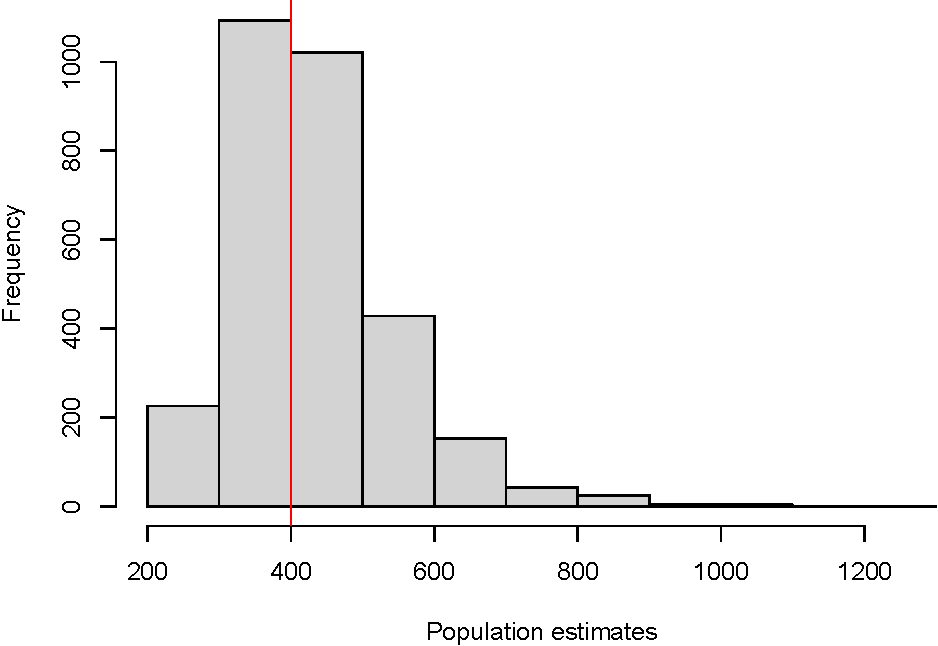
\includegraphics[width=0.9\linewidth]{bookdown_files/figure-latex/BayesMR-1} \caption{Estimated posterior distribution for population size; red line indicates true value.}\label{fig:BayesMR}
\end{figure}

The jagsfit object is a data frame that can be inspected in the Environment window. Note that sims.list arrays contain 3000 elements, which is the combined length of 1000 retained values (2000-n.burnin) from each of three chains. (When entering a jagsfit object in the Source window or Console, typing \$ after each level of the object will bring up an RStudio prompt for the next choice.)

The model results include pD\index{pD}, which is an estimate of the number of effective parameters in the model. In simple models, we can often count the number of nominal parameters, but the number of effective parameters may be less; for example, parameters may be correlated or constrained by an informative prior distribution \citep{mccarthy2007}. JAGS uses numerical methods to estimate pD. For this model, we would expect pD to be close to 1 for the estimate of N.hat; MarkedFraction is a calculated value and not a model parameter.

JAGS also provides an estimate of the Deviance Information Criterion\index{Information Criterion, Deviance} (DIC), which is a relative measure of how well a model fits the data \citep{mccarthy2007, lunn.etal2009}. It is the Bayesian analog of the Akaike's Information Criterion\index{Information Criterion, Akaike's} (AIC) that is widely used in a frequentist setting to compare alternative models. Like the AIC, the DIC results in a trade-off between model fit (likelihood) and complexity (number of parameters) \citep{mccarthy2007}. The DIC score is calculated using a measure of fit (deviance at the mean of the posterior distribution) and a measure of model complexity (pD); lower values are better when comparing alternative models. DIC scores should be interpreted with caution because of the difficulty in estimating pD for some models \citep{lunn.etal2009}.

It is worth noting that this model may also be fit by using MarkedFraction as the model parameter. It is easy to specify the uninformative prior distribution (and initial values) in this case, as MarkedFraction is a proportion between 0 and 1. Now N.hat is a calculated value. One major advantage of Bayesian software is that we automatically get full information about parameters that are calculated functions of model parameters. In this case, the calculated value (N.hat) is of primary interest, rather than the actual model parameter MarkedFraction. Results for Nhat characterize its posterior distribution, which takes into account the prior information (none here) and the new data.

\begin{Shaded}
\begin{Highlighting}[]
\FunctionTok{rm}\NormalTok{(}\AttributeTok{list=}\FunctionTok{ls}\NormalTok{()) }\CommentTok{\# Clear Environment}

\CommentTok{\# Load necessary library packages}
\FunctionTok{library}\NormalTok{(rjags)   }\CommentTok{\# Package for fitting JAGS models from within R}
\FunctionTok{library}\NormalTok{(R2jags)  }\CommentTok{\# Package for fitting JAGS models. Requires rjags}

\CommentTok{\# Arbitrary \textquotesingle{}observed\textquotesingle{} values for analysis}
\NormalTok{N.true }\OtherTok{\textless{}{-}} \DecValTok{400}  \CommentTok{\# Population size}
\NormalTok{p.true }\OtherTok{\textless{}{-}} \FloatTok{0.2} \CommentTok{\# Capture probability (fraction of population sampled)}
\NormalTok{n1 }\OtherTok{\textless{}{-}}\NormalTok{ N.true }\SpecialCharTok{*}\NormalTok{ p.true }\CommentTok{\# Number caught and marked in first sample}
\NormalTok{n2 }\OtherTok{\textless{}{-}}\NormalTok{ N.true }\SpecialCharTok{*}\NormalTok{ p.true }\CommentTok{\# Number caught and examined for marks in second sample}
\NormalTok{m2 }\OtherTok{\textless{}{-}}\NormalTok{ n2 }\SpecialCharTok{*}\NormalTok{ p.true }\CommentTok{\# Number of marked fish in second sample}

\CommentTok{\# JAGS code}
\FunctionTok{sink}\NormalTok{(}\StringTok{"TwoSampleCR.txt"}\NormalTok{)}
\FunctionTok{cat}\NormalTok{(}\StringTok{"}
\StringTok{    model \{}

\StringTok{    \# Priors}
\StringTok{    MarkedFraction \textasciitilde{} dunif(0, 1)}

\StringTok{    \# Calculated value}
\StringTok{    N.hat \textless{}{-} n1 /MarkedFraction}

\StringTok{    \# Likelihood}
\StringTok{    \# Binomial distribution for observed recaptures}
\StringTok{    m2 \textasciitilde{} dbin(MarkedFraction, n2)}
\StringTok{    \}}

\StringTok{    "}\NormalTok{,}\AttributeTok{fill =} \ConstantTok{TRUE}\NormalTok{)}
\FunctionTok{sink}\NormalTok{()}

\CommentTok{\# Bundle data}
\NormalTok{jags.data }\OtherTok{\textless{}{-}} \FunctionTok{list}\NormalTok{(}\StringTok{"n1"}\NormalTok{, }\StringTok{"n2"}\NormalTok{, }\StringTok{"m2"}\NormalTok{)}

\CommentTok{\# Initial values.}
\NormalTok{jags.inits }\OtherTok{\textless{}{-}} \ControlFlowTok{function}\NormalTok{()\{ }\FunctionTok{list}\NormalTok{(}\AttributeTok{MarkedFraction=}\FunctionTok{runif}\NormalTok{(}\DecValTok{1}\NormalTok{, }\AttributeTok{min=}\DecValTok{0}\NormalTok{, }\AttributeTok{max=}\DecValTok{1}\NormalTok{))\}}

\NormalTok{model.file }\OtherTok{\textless{}{-}} \StringTok{\textquotesingle{}TwoSampleCR.txt\textquotesingle{}}

\CommentTok{\# Parameters monitored}
\NormalTok{jags.params }\OtherTok{\textless{}{-}} \FunctionTok{c}\NormalTok{(}\StringTok{"N.hat"}\NormalTok{, }\StringTok{"MarkedFraction"}\NormalTok{)}

\CommentTok{\# Call JAGS from R}
\NormalTok{jagsfit }\OtherTok{\textless{}{-}} \FunctionTok{jags}\NormalTok{(}\AttributeTok{data=}\NormalTok{jags.data, }\AttributeTok{inits=}\NormalTok{jags.inits, jags.params,}
                \AttributeTok{n.chains =} \DecValTok{3}\NormalTok{, }\AttributeTok{n.thin =} \DecValTok{1}\NormalTok{, }\AttributeTok{n.iter =} \DecValTok{2000}\NormalTok{, }\AttributeTok{n.burnin =} \DecValTok{1000}\NormalTok{,}
\NormalTok{                model.file)}
\FunctionTok{print}\NormalTok{(jagsfit, }\AttributeTok{digits=}\DecValTok{3}\NormalTok{)}
\FunctionTok{plot}\NormalTok{(jagsfit)}
\end{Highlighting}
\end{Shaded}

Another advantage of this way of parameterizing the model is that we avoid specifying an arbitrary upper bound for initial values for N.hat. Results of the two approaches are similar.

\hypertarget{Debug}{%
\subsection{Debugging code}\label{Debug}}

Anyone who develops new code for fisheries data analysis will wrestle with the inevitable coding errors, not only in JAGS but also the R code that surrounds it. Let's begin by looking at a few examples of R coding errors:

\begin{Shaded}
\begin{Highlighting}[]
\FunctionTok{rm}\NormalTok{(}\AttributeTok{list=}\FunctionTok{ls}\NormalTok{()) }\CommentTok{\# Clear Environment}

\CommentTok{\#1}
\NormalTok{x }\OtherTok{\textless{}{-}} \DecValTok{2}
\FunctionTok{lg}\NormalTok{(x) }\CommentTok{\# Incorrect function name}

\CommentTok{\#2}
\NormalTok{y }\OtherTok{\textless{}{-}} \DecValTok{4}
\NormalTok{z }\OtherTok{\textless{}{-}}\NormalTok{ x}\SpecialCharTok{+}\NormalTok{y }\CommentTok{\# Typo (should have been x*y)}

\CommentTok{\#3}
\NormalTok{RandLength }\OtherTok{\textless{}{-}} \FunctionTok{rnorm}\NormalTok{(}\DecValTok{1}\NormalTok{, }\DecValTok{10}\NormalTok{, }\DecValTok{2}\NormalTok{) }\CommentTok{\# Correct but poorly documented}
\NormalTok{RandLength }\OtherTok{\textless{}{-}} \FunctionTok{rnorm}\NormalTok{(}\DecValTok{10}\NormalTok{,}\DecValTok{2}\NormalTok{) }\CommentTok{\# Sample size omitted}
\NormalTok{RandLength }\OtherTok{\textless{}{-}} \FunctionTok{rnorm}\NormalTok{(}\DecValTok{1}\NormalTok{,}\DecValTok{10}\NormalTok{) }\CommentTok{\# sd omitted so default used (incorrectly)}
\NormalTok{RandLength }\OtherTok{\textless{}{-}} \FunctionTok{rnorm}\NormalTok{(}\AttributeTok{n=}\DecValTok{1}\NormalTok{, }\AttributeTok{mean=}\DecValTok{10}\NormalTok{, }\AttributeTok{sd=}\DecValTok{2}\NormalTok{) }\CommentTok{\# Correct and fully documented}

\CommentTok{\#4}
\NormalTok{x2 }\OtherTok{\textless{}{-}} \FunctionTok{rnorm}\NormalTok{(}\AttributeTok{n=}\DecValTok{1000}\NormalTok{, }\AttributeTok{mean=}\DecValTok{10}\NormalTok{, }\AttributeTok{sd=}\DecValTok{5}\NormalTok{)}
\NormalTok{x3 }\OtherTok{\textless{}{-}} \FunctionTok{rnorm}\NormalTok{(}\AttributeTok{n=}\DecValTok{1000}\NormalTok{, }\AttributeTok{mean=}\DecValTok{20}\NormalTok{, }\AttributeTok{sd=}\DecValTok{10}\NormalTok{)}
\NormalTok{x4 }\OtherTok{\textless{}{-}}\NormalTok{ x2}\SpecialCharTok{+}\NormalTok{x3}
\FunctionTok{mean}\NormalTok{(x4)}
\FunctionTok{var}\NormalTok{(x4)}
\end{Highlighting}
\end{Shaded}

The first example is easy to resolve, as we get a helpful error message in the Console. Rechecking the code, or doing an internet search for the correct function name, are approaches for addressing this type of error. The second example, if our intent was to assign x*y to z, is much more dangerous. The code will run but will give the wrong answer because of a typing error. It is always essential to review new code, line by line. Having a colleague (fresh set of eyes) check code can also be productive. R code can often be executed line by line, and checking calculated values in the Environment window can help in finding this sort of logic error, at least for simpler analyses.

In the third example, we are simulating a random length observation, drawn from a normal distribution with a mean of 10 and standard deviation of 2. The first version of the code works correctly but is poorly documented. The second example runs but does not produce the intended result. We omitted the first argument and did not include parameter names, so R assumes incorrectly that the first argument is the sample size and the second one is the mean. The third argument is missing so R uses the default value (sd=1), which in this case is incorrect. Even if we wanted to use an sd of 1, it is better to specify it for clarity. RStudio is helpful in working with functions in that it displays the function arguments and any defaults, once the function name and ``('' have been entered. The fourth version works as intended, and makes clear the values that are being used.

The fourth example is coded correctly but illustrates another way of checking code. Simulation makes it easy to use a large sample size, to check sample statistics for x4. We verify that the mean is close to the expected value (10+20). The variance of a sum equals the sum of the variances so we confirm that the sample variance is close to the expected value (25+100).

How many errors do you find in the following section of code? Review line by line and correct errors before executing the code. Once the code is working correctly, confirm that the sample median is very close to the expected population size:

\begin{Shaded}
\begin{Highlighting}[]
\FunctionTok{rm}\NormalTok{(}\AttributeTok{list=}\FunctionTok{ls}\NormalTok{()) }\CommentTok{\# Clear Environment}

\CommentTok{\# Two{-}sample population estimate}
\NormalTok{N.true }\OtherTok{\textless{}{-}} \DecValTok{400}  \CommentTok{\# Arbitrary assumed population size}
\NormalTok{p.true }\OtherTok{\textless{}{-}}\SpecialCharTok{{-}} \FloatTok{0.2} \CommentTok{\# Capture probability (fraction of population sampled)}
\NormalTok{n1 }\OtherTok{\textless{}{-}}\NormalTok{ N.true X p.true }\CommentTok{\# Number caught and marked in first sample}
\NormalTok{n2 }\OtherTok{\textless{}{-}}\NormalTok{ N.true }\SpecialCharTok{*}\NormalTok{ p.true }\CommentTok{\# Number caught and examined for marks in second sample}

\NormalTok{Reps }\OtherTok{\textless{}{-}} \DecValTok{1000}
\NormalTok{m2.vec }\OtherTok{\textless{}{-}} \FunctionTok{rbinom}\NormalTok{(}\AttributeTok{n=}\NormalTok{Rep, }\AttributeTok{prob=}\NormalTok{n1}\SpecialCharTok{/}\NormalTok{N.true, }\AttributeTok{size=}\NormalTok{n2)}
\NormalTok{N.hat }\OtherTok{\textless{}{-}}\NormalTok{ n1 }\SpecialCharTok{*}\NormalTok{ n2 }\SpecialCharTok{/}\NormalTok{ m2.vec}
\FunctionTok{hist}\NormalTok{(N.hat, }\AttributeTok{xlab=}\StringTok{"Population estimate"}\NormalTok{, }\AttributeTok{main=}\StringTok{""}\NormalTok{)}
\FunctionTok{mean}\NormalTok{(Nhat)}
\FunctionTok{quantile}\NormalTok{(N.hat, }\AttributeTok{probs=}\FunctionTok{c}\NormalTok{(}\FloatTok{0.5}\NormalTok{), }\AttributeTok{na.rm=}\ConstantTok{TRUE}\NormalTok{)}\ErrorTok{)}  \CommentTok{\# Sample median}
\end{Highlighting}
\end{Shaded}

Debugging JAGS code can be more challenging. There is no option for executing single lines of code as is possible with R. It is usually a matter of fixing one error at a time until the code runs, then checking and testing the code to be confident that it is working correctly. Consider the following (correctly coded) example for a tagging study to estimate the exploitation rate (fraction of the population harvested). Our simulation generates the single observation for the number of tags returned (e.g., over a year). This observation is drawn from a binomial distribution and we use the same JAGS function (dbin()) as in the population estimate examples:

\begin{Shaded}
\begin{Highlighting}[]
\FunctionTok{rm}\NormalTok{(}\AttributeTok{list=}\FunctionTok{ls}\NormalTok{()) }\CommentTok{\# Clear Environment}

\CommentTok{\# Arbitrary \textquotesingle{}observed\textquotesingle{} values for analysis}
\NormalTok{N.tagged }\OtherTok{\textless{}{-}} \DecValTok{100}
\NormalTok{Exp.rate }\OtherTok{\textless{}{-}} \FloatTok{0.4}
\NormalTok{Tags.returned }\OtherTok{\textless{}{-}} \FunctionTok{rbinom}\NormalTok{(}\AttributeTok{n=}\DecValTok{1}\NormalTok{, }\AttributeTok{prob=}\NormalTok{Exp.rate, }\AttributeTok{size=}\NormalTok{N.tagged)}

\CommentTok{\# Load necessary library packages}
\FunctionTok{library}\NormalTok{(rjags)   }\CommentTok{\# Package for fitting JAGS models from within R}
\FunctionTok{library}\NormalTok{(R2jags)  }\CommentTok{\# Package for fitting JAGS models. Requires rjags}

\CommentTok{\# JAGS code}
\FunctionTok{sink}\NormalTok{(}\StringTok{"ExpRate.txt"}\NormalTok{)}
\FunctionTok{cat}\NormalTok{(}\StringTok{"}
\StringTok{    model \{}

\StringTok{    \# Priors}
\StringTok{    Exp.rate.est \textasciitilde{} dunif(0,1)}

\StringTok{    \# Likelihood}
\StringTok{    Tags.returned \textasciitilde{} dbin(Exp.rate.est, N.tagged)}
\StringTok{\}}
\StringTok{    "}\NormalTok{,}\AttributeTok{fill =} \ConstantTok{TRUE}\NormalTok{)}
\FunctionTok{sink}\NormalTok{()}

\CommentTok{\# Bundle data}
\NormalTok{jags.data }\OtherTok{\textless{}{-}} \FunctionTok{list}\NormalTok{(}\StringTok{"N.tagged"}\NormalTok{, }\StringTok{"Tags.returned"}\NormalTok{)}

\CommentTok{\# Initial values.}
\NormalTok{jags.inits }\OtherTok{\textless{}{-}} \ControlFlowTok{function}\NormalTok{()\{ }\FunctionTok{list}\NormalTok{(}\AttributeTok{Exp.rate.est=}\FunctionTok{runif}\NormalTok{(}\AttributeTok{n=}\DecValTok{1}\NormalTok{, }\AttributeTok{min=}\DecValTok{0}\NormalTok{, }\AttributeTok{max=}\DecValTok{1}\NormalTok{))\}}

\NormalTok{model.file }\OtherTok{\textless{}{-}} \StringTok{\textquotesingle{}ExpRate.txt\textquotesingle{}}

\CommentTok{\# Parameters monitored}
\NormalTok{jags.params }\OtherTok{\textless{}{-}} \FunctionTok{c}\NormalTok{(}\StringTok{"Exp.rate.est"}\NormalTok{)}

\CommentTok{\# Call JAGS from R}
\NormalTok{jagsfit }\OtherTok{\textless{}{-}} \FunctionTok{jags}\NormalTok{(}\AttributeTok{data=}\NormalTok{jags.data, }\AttributeTok{inits=}\NormalTok{jags.inits, jags.params,}
                \AttributeTok{n.chains =} \DecValTok{3}\NormalTok{, }\AttributeTok{n.thin =} \DecValTok{1}\NormalTok{, }\AttributeTok{n.iter =} \DecValTok{2000}\NormalTok{, }\AttributeTok{n.burnin =} \DecValTok{1000}\NormalTok{,}
\NormalTok{                model.file)}
\FunctionTok{print}\NormalTok{(jagsfit, }\AttributeTok{digits=}\DecValTok{3}\NormalTok{)}
\FunctionTok{plot}\NormalTok{(jagsfit)}
\end{Highlighting}
\end{Shaded}

Begin by running the code as is, then try substituting each of the following (incorrect) lines, one at a time.

\begin{itemize}
\tightlist
\item
  \texttt{ExpRate.est\ \textasciitilde{}\ dunif(0,1)}
\item
  \texttt{Exp.rate.est\ \textasciitilde{}\ unif(0,1)}
\item
  \texttt{Tags.returned\ \textasciitilde{}\ dbin(Exp.rate.est)}
\end{itemize}

The first error message points to line 8. JAGS correctly reports that the variable Exp.rate.est has not been previously defined. This is correct, but the error is actually on line 5, where the intended parameter name (Exp.rate.est) was mistyped. The second error is easy to diagnose because it specifies that the ``unif'' distribution on line 5 is unknown. The third error indicates that a discrete-valued parameter for function dbin() is missing. This makes sense because the size of the experiment (N.tagged) was omitted.

As with R code, the first step is always to review the code line by line. Fitting a model to simulated data is always useful (even if there are field observations) because the correct answer is known. Another strategy is to start with the simplest possible analysis, then add complexity one piece at a time. For example, \citet{kéry.schaub_2011} discuss Cormack-Jolly-Seber models for estimating survival, beginning with constant parameters then gradually adding more complexity (e.g., models that allow for time and individual variation).

Skill in debugging comes with experience. It is hoped that the above strategies will be useful in working through the inevitable coding errors.

\hypertarget{Convergence}{%
\subsection{Judging convergence}\label{Convergence}}

The MCMC process is iterative so it is important to ensure that the number of updates (iterations) is sufficient to achieve convergence. One practical approach is to fit the model with some arbitrary (but reasonably large) number of updates, then refit the model using larger numbers of updates. Results that are stable suggest that convergence has been achieved. The convergence statistic Rhat \citep{gelman.rubin1992, brooks.gelman1998, lunn.etal2012} is also generally reliable as a measure of convergence. It compares between- and within-chain variance; their ratio should be close to 1 once chains have converged. Especially for models for which convergence appears to be slow, it can also be helpful to view ``trace'' plots that show how estimates change as updating occurs \citep{kéry_2010}. Add the following lines of code to the two-sample mark-recapture model used in Section \ref{JAGS-model-fit}:

\begin{Shaded}
\begin{Highlighting}[]
\FunctionTok{par}\NormalTok{(}\AttributeTok{mfrow=}\FunctionTok{c}\NormalTok{(}\DecValTok{3}\NormalTok{,}\DecValTok{1}\NormalTok{)) }\CommentTok{\# Multi{-}frame plot, 3 rows, 1 col}
\FunctionTok{matplot}\NormalTok{(jagsfit}\SpecialCharTok{$}\NormalTok{BUGSoutput}\SpecialCharTok{$}\NormalTok{sims.array[,,}\DecValTok{1}\NormalTok{], }\AttributeTok{type =} \StringTok{"l"}\NormalTok{, }\AttributeTok{ylab=}\StringTok{"Marked fraction"}\NormalTok{)}
\FunctionTok{matplot}\NormalTok{(jagsfit}\SpecialCharTok{$}\NormalTok{BUGSoutput}\SpecialCharTok{$}\NormalTok{sims.array[,,}\DecValTok{2}\NormalTok{], }\AttributeTok{type =} \StringTok{"l"}\NormalTok{, }\AttributeTok{ylab=}\StringTok{"N hat"}\NormalTok{)}
\FunctionTok{matplot}\NormalTok{(jagsfit}\SpecialCharTok{$}\NormalTok{BUGSoutput}\SpecialCharTok{$}\NormalTok{sims.array[,,}\DecValTok{3}\NormalTok{], }\AttributeTok{type =} \StringTok{"l"}\NormalTok{, }\AttributeTok{ylab=}\StringTok{"Deviance"}\NormalTok{)}

\NormalTok{jagsfit.mcmc }\OtherTok{\textless{}{-}} \FunctionTok{as.mcmc}\NormalTok{(jagsfit) }\CommentTok{\# Creates an MCMC object for plotting}
\FunctionTok{plot}\NormalTok{(jagsfit.mcmc) }\CommentTok{\# Trace and density plots}
\end{Highlighting}
\end{Shaded}

The first approach follows an example from \citet{kéry_2010}. We use the par() graphical function to set up a multi-frame plot (by row), with three rows and one column. This results in a compact set of three plots within a single RStudio plot window. The next three lines use the built-in matplot() function to plot columns of a matrix as overlaid lines. The Environment window can be viewed to see the structure of the sims.array, a matrix of type num{[}1:1000, 1:3, 1:3{]}. The first dimension is for the 1000 retained updates, the second is for chains 1-3, and the third is for the variable (MarkedFraction, Nhat, Deviance). Omitting the ranges for updates and chains results in a plot containing all updates, with a different colored line for each chain. We could also specify a subset of the range to see the initial pattern (e.g., \ldots sims.array{[}1:100,,1{]}, \ldots). For this simple model, the estimates converge almost immediately so there is no obvious transitory pattern. Note that there is a lot of wasted space and it may be necessary to increase the size of the Plots window to see the plots adequately.

The next two of code provide a more automated way of generating trace and density plots, using methods contained in the \textbf{coda} \citep{R-coda} package (loaded automatically by rjags). The as.mcmc() function converts the original output object (jagsfit) into an MCMC object. The plot function here produces a nicely formatted set of trace and density plots that are very helpful in confirming convergence. If convergence has been achieved, the trace plots should appear to be a ``grassy lawn'' or ``fuzzy caterpillar'' without any trend, with overlapping (fully mixed) chains. Density plots show the estimated posterior distributions, and given convergence, should have an essentially identical pattern for the three chains. Convergence occurs very quickly here but we will see in later chapters with more complex models that convergence can sometimes be more difficult to achieve.

\hypertarget{Likelihood}{%
\subsection{What is a likelihood?}\label{Likelihood}}

As mentioned above, Bayesian software uses the likelihood and prior information to estimate the posterior distribution. But what exactly is a likelihood? It is an expression or function that is used to estimate the \emph{likelihood} of obtaining the sample observation(s), given some specific value for each model parameter. As an example, let's return to the second version of the mark-recapture analysis, with the single model parameter MarkedFracton (the fraction of the population that is marked). We use the binomial distribution to model the number of recaptures. The likelihood function for the binomial is the same as the probability distribution: \(L(p | n, k) = {n \choose k} p^{k} (1-p)^{n-k}\), except that here, we estimate the likelihood of a certain value for p, given k successes in a trial of size n.~We can look at likelihoods using the same parameter values as in the simulation:

\begin{Shaded}
\begin{Highlighting}[]
\FunctionTok{rm}\NormalTok{(}\AttributeTok{list=}\FunctionTok{ls}\NormalTok{()) }\CommentTok{\# Clear Environment}

\CommentTok{\# Arbitrary \textquotesingle{}observed\textquotesingle{} values for analysis}
\NormalTok{N.true }\OtherTok{\textless{}{-}} \DecValTok{400}  \CommentTok{\# Population size}
\NormalTok{p.true }\OtherTok{\textless{}{-}} \FloatTok{0.2} \CommentTok{\# Capture probability (fraction of population sampled)}
\NormalTok{n1 }\OtherTok{\textless{}{-}}\NormalTok{ N.true }\SpecialCharTok{*}\NormalTok{ p.true }\CommentTok{\# Number caught and marked in first sample}
\NormalTok{n2 }\OtherTok{\textless{}{-}}\NormalTok{ N.true }\SpecialCharTok{*}\NormalTok{ p.true }\CommentTok{\# Number caught and examined for marks in second sample}
\NormalTok{m2 }\OtherTok{\textless{}{-}}\NormalTok{ n2 }\SpecialCharTok{*}\NormalTok{ p.true }\CommentTok{\# Number of marked fish in second sample}

\CommentTok{\# Calculate likelihood for specific value of p}
\NormalTok{p }\OtherTok{\textless{}{-}} \FloatTok{0.2}
\FunctionTok{choose}\NormalTok{(n2,m2) }\SpecialCharTok{*}\NormalTok{ p}\SpecialCharTok{\^{}}\NormalTok{m2 }\SpecialCharTok{*}\NormalTok{ (}\DecValTok{1}\SpecialCharTok{{-}}\NormalTok{p)}\SpecialCharTok{\^{}}\NormalTok{(n2}\SpecialCharTok{{-}}\NormalTok{m2) }\CommentTok{\# Likelihood for single value of p}

\FunctionTok{dbinom}\NormalTok{(}\AttributeTok{x=}\NormalTok{m2, }\AttributeTok{size=}\NormalTok{n2, }\AttributeTok{prob=}\NormalTok{p) }\CommentTok{\# x successes, built{-}in function to obtain same result}

\CommentTok{\# Create vector of possible p values, determine likelihood for each}
\NormalTok{p }\OtherTok{\textless{}{-}} \FunctionTok{seq}\NormalTok{(}\AttributeTok{from=}\FloatTok{0.02}\NormalTok{, }\AttributeTok{to=}\DecValTok{1}\NormalTok{, }\AttributeTok{by=}\FloatTok{0.02}\NormalTok{)}
\NormalTok{l.vec }\OtherTok{\textless{}{-}} \FunctionTok{choose}\NormalTok{(n2,m2) }\SpecialCharTok{*}\NormalTok{ p}\SpecialCharTok{\^{}}\NormalTok{m2 }\SpecialCharTok{*}\NormalTok{ (}\DecValTok{1}\SpecialCharTok{{-}}\NormalTok{p)}\SpecialCharTok{\^{}}\NormalTok{(n2}\SpecialCharTok{{-}}\NormalTok{m2)}
\FunctionTok{par}\NormalTok{(}\AttributeTok{mfrow=}\FunctionTok{c}\NormalTok{(}\DecValTok{1}\NormalTok{,}\DecValTok{1}\NormalTok{)) }\CommentTok{\# Reset plot frame}
\FunctionTok{plot}\NormalTok{(p, l.vec, }\AttributeTok{ylab=}\StringTok{"Likelihood"}\NormalTok{, }\AttributeTok{col=}\StringTok{"red"}\NormalTok{)}

\CommentTok{\# Examine change in likelihood at higher number of recaptures}
\NormalTok{new.m2 }\OtherTok{\textless{}{-}} \DecValTok{18}
\NormalTok{new.l.vec }\OtherTok{\textless{}{-}} \FunctionTok{choose}\NormalTok{(n2,new.m2) }\SpecialCharTok{*}\NormalTok{ p}\SpecialCharTok{\^{}}\NormalTok{new.m2 }\SpecialCharTok{*}\NormalTok{ (}\DecValTok{1}\SpecialCharTok{{-}}\NormalTok{p)}\SpecialCharTok{\^{}}\NormalTok{(n2}\SpecialCharTok{{-}}\NormalTok{new.m2)}
\FunctionTok{points}\NormalTok{(p, new.l.vec, }\AttributeTok{col=}\StringTok{"blue"}\NormalTok{)}
\end{Highlighting}
\end{Shaded}

The likelihood calculation at p=0.2 uses the choose() function, to determine how many ways m2=16 recaptures can be drawn from a sample of size 80. Type \texttt{choose(n2,m2)} in the Console to see that it is a very large number! The remainder of the expression determines the probability of 16 successes and 80-16 failures. We can obtain the same result from the built-in function dbinom(), although it seems more instructive to write out the full expression.

The calculated likelihood (0.11) is really only of interest as a relative value, compared to other potential values for p.~We use the seq() function to create a vector of potential p values, and obtain a vector of likelihoods from the p vector. Plotting the points shows that the likelihood peaks sharply at 0.2 (not surprisingly since that is the value that generated the 16 recaptures) and decreases to near 0 at about 0.08 and 0.32.

We have assumed thus far that we obtained the expected number of recaptures (80*p), but in reality, the number of recaptures would be a binomially-distributed random variate. A different observed value for m\textsubscript{2} would shift the likelihood function. The next lines of code calculate the likelihood for a slightly higher number of recaptures. The points function adds the new likelihood values to the plot, using the col=``blue'' plot option. The new values are shifted to the right because the number of recaptured fish was higher.

If multiple independent samples are taken, the combined likelihood is a product. For our two assumed samples of 80 fish, with 16 recaptures in one and 18 in the other, the combined likelihood at each level of p would be the product l.vec * new.l.vec.

We wrote out the expression for the likelihood for this example, but that is not needed when using the BUGS language. We need only specify the function name for the distribution describing our sample data. JAGS does the behind-the-scenes work to provide the code for the likelihood function. Working at a higher level allows us to focus on the study design and assumptions, which guide us to our choice of sample distribution.

\hypertarget{Deviance}{%
\subsection{Deviance as a measure of model fit}\label{Deviance}}

Likelihood calculations were introduced in Section \ref{Likelihood}. Here we show two related measures of model fit (log-likelihood and deviance) using the same mark-recapture example. There can be computational advantages to working with the log-likelihood compared to the likelihood \citep{mccarthy2007}.

\begin{Shaded}
\begin{Highlighting}[]
\FunctionTok{rm}\NormalTok{(}\AttributeTok{list=}\FunctionTok{ls}\NormalTok{()) }\CommentTok{\# Clear Environment}

\CommentTok{\# Arbitrary \textquotesingle{}observed\textquotesingle{} values for analysis}
\NormalTok{N.true }\OtherTok{\textless{}{-}} \DecValTok{400}  \CommentTok{\# Population size}
\NormalTok{p.true }\OtherTok{\textless{}{-}} \FloatTok{0.2} \CommentTok{\# Capture probability (fraction of population sampled)}
\NormalTok{n1 }\OtherTok{\textless{}{-}}\NormalTok{ N.true }\SpecialCharTok{*}\NormalTok{ p.true }\CommentTok{\# Number caught and marked in first sample}
\NormalTok{n2 }\OtherTok{\textless{}{-}}\NormalTok{ N.true }\SpecialCharTok{*}\NormalTok{ p.true }\CommentTok{\# Number caught and examined for marks in second sample}
\NormalTok{m2 }\OtherTok{\textless{}{-}}\NormalTok{ n2 }\SpecialCharTok{*}\NormalTok{ p.true }\CommentTok{\# Number of marked fish in second sample}

\CommentTok{\# Create vector of possible p values, determine likelihood for each}
\NormalTok{p }\OtherTok{\textless{}{-}} \FunctionTok{seq}\NormalTok{(}\AttributeTok{from=}\FloatTok{0.02}\NormalTok{, }\AttributeTok{to=}\DecValTok{1}\NormalTok{, }\AttributeTok{by=}\FloatTok{0.02}\NormalTok{)}
\NormalTok{l.vec }\OtherTok{\textless{}{-}} \FunctionTok{choose}\NormalTok{(n2,m2) }\SpecialCharTok{*}\NormalTok{ p}\SpecialCharTok{\^{}}\NormalTok{m2 }\SpecialCharTok{*}\NormalTok{ (}\DecValTok{1}\SpecialCharTok{{-}}\NormalTok{p)}\SpecialCharTok{\^{}}\NormalTok{(n2}\SpecialCharTok{{-}}\NormalTok{m2)}
\FunctionTok{plot}\NormalTok{(p, l.vec, }\AttributeTok{ylab=}\StringTok{"Likelihood"}\NormalTok{, }\AttributeTok{col=}\StringTok{"red"}\NormalTok{)}

\NormalTok{log\_l.vec }\OtherTok{\textless{}{-}} \FunctionTok{log}\NormalTok{(l.vec) }\CommentTok{\# Log{-}likelihood}
\FunctionTok{plot}\NormalTok{(p, log\_l.vec, }\AttributeTok{ylab=}\StringTok{"log{-}Likelihood"}\NormalTok{, }\AttributeTok{col=}\StringTok{"red"}\NormalTok{)}
\NormalTok{dev.vec }\OtherTok{\textless{}{-}} \SpecialCharTok{{-}}\DecValTok{2} \SpecialCharTok{*}\NormalTok{ log\_l.vec }\CommentTok{\# Deviance ({-}2 * ln\_L)}
\FunctionTok{plot}\NormalTok{(p, dev.vec, }\AttributeTok{ylab=}\StringTok{"Deviance"}\NormalTok{, }\AttributeTok{col=}\StringTok{"red"}\NormalTok{)}
\end{Highlighting}
\end{Shaded}

Compared to the likelihood, the log-likelihood curve has a different shape but the same peak at p=0.2 (the most likely value given 16 successes in a trial size of 80). The deviance is obtained by multiplying the log-likelihood by -2. The plotted pattern is now inverted so that now the curve has a \emph{minimum} at p=0.2; i.e., a larger value for deviance indicates a poorer fit \citep{mccarthy2007}. JAGS uses the deviance to obtain parameter estimates, but it is nice to know that we would obtain the same estimates from either the maximum likelihood or log-likelihood or the minimum deviance \citep{mccarthy2007}.

\hypertarget{Model-checking}{%
\subsection{Model checking}\label{Model-checking}}

It is easy to fit the correct model to simulated data, but that is not the case for real (field) data. Any model fit to field data should be viewed as an approximation of the underlying ecological processes. We cannot prove that the model is correct, but we can examine whether it is a useful approximation. One method for doing this is the posterior predictive check \citep{kéry_2010, kéry.schaub_2011, gelman.etal_2013, conn.etal_2018}. This method compares a measure of fit for replicated data generated under the fitted model compared to observed data. If the measure of fit (e.g., sum of squares or chi-square) is markedly different (usually higher) for the observed data, that suggests that the observed data contain some features not captured by the fitted model.

Our first example uses simulated catch data from a Poisson distribution, as might be obtained by standardized electrofishing or trawling. Keep in mind that these are our ``observed'' catches, to be compared with replicate data obtained by simulation. We arbitrarily set the mean for the Poisson distribution at 7 and the sample size at 30. Before viewing the extended JAGS code that includes the posterior predictive check, let's examine a version that simply fits the model:

\begin{Shaded}
\begin{Highlighting}[]
\CommentTok{\# Fit model to catch data from Poisson distribution}

\FunctionTok{rm}\NormalTok{(}\AttributeTok{list=}\FunctionTok{ls}\NormalTok{()) }\CommentTok{\# Clear Environment}

\NormalTok{N }\OtherTok{\textless{}{-}} \DecValTok{30}
\NormalTok{mu }\OtherTok{\textless{}{-}} \DecValTok{7}
\NormalTok{Catch }\OtherTok{\textless{}{-}} \FunctionTok{rpois}\NormalTok{(}\AttributeTok{n=}\NormalTok{N, }\AttributeTok{lambda=}\NormalTok{mu) }\CommentTok{\# Catches drawn from Poisson distribution}
\NormalTok{Freq }\OtherTok{\textless{}{-}} \FunctionTok{table}\NormalTok{(Catch)  }\CommentTok{\# Distribution of simulated catches}
\FunctionTok{barplot}\NormalTok{(Freq, }\AttributeTok{main=}\StringTok{""}\NormalTok{, }\AttributeTok{xlab=}\StringTok{"Catch"}\NormalTok{, }\AttributeTok{ylab=}\StringTok{"Frequency"}\NormalTok{)}

\CommentTok{\# Load necessary library}
\FunctionTok{library}\NormalTok{(rjags)}
\FunctionTok{library}\NormalTok{(R2jags)}

\FunctionTok{sink}\NormalTok{(}\StringTok{"PoissonFit.txt"}\NormalTok{)}
\FunctionTok{cat}\NormalTok{(}\StringTok{"}
\StringTok{model \{}

\StringTok{\# Prior}
\StringTok{ lambda.est \textasciitilde{} dunif(0, 100)}

\StringTok{\# Likelihood}
\StringTok{    for(i in 1:N) \{}
\StringTok{      Catch[i] \textasciitilde{} dpois(lambda.est)}
\StringTok{      \} \#y}
\StringTok{\}}
\StringTok{    "}\NormalTok{,}\AttributeTok{fill=}\ConstantTok{TRUE}\NormalTok{)}
\FunctionTok{sink}\NormalTok{()}

\CommentTok{\# Bundle data}
\NormalTok{jags.data }\OtherTok{\textless{}{-}} \FunctionTok{list}\NormalTok{(}\StringTok{"N"}\NormalTok{, }\StringTok{"Catch"}\NormalTok{)}

\CommentTok{\# Initial values}
\NormalTok{jags.inits }\OtherTok{\textless{}{-}} \ControlFlowTok{function}\NormalTok{()\{ }\FunctionTok{list}\NormalTok{(}\AttributeTok{lambda.est=}\FunctionTok{runif}\NormalTok{(}\AttributeTok{n=}\DecValTok{1}\NormalTok{, }\AttributeTok{min=}\DecValTok{0}\NormalTok{, }\AttributeTok{max=}\DecValTok{100}\NormalTok{))\}}

\NormalTok{model.file }\OtherTok{\textless{}{-}} \StringTok{\textquotesingle{}PoissonFit.txt\textquotesingle{}}

\CommentTok{\# Parameters monitored}
\NormalTok{jags.params }\OtherTok{\textless{}{-}} \FunctionTok{c}\NormalTok{(}\StringTok{"lambda.est"}\NormalTok{)}

\CommentTok{\# Call JAGS from R}
\NormalTok{jagsfit }\OtherTok{\textless{}{-}} \FunctionTok{jags}\NormalTok{(}\AttributeTok{data=}\NormalTok{jags.data, jags.params, }\AttributeTok{inits=}\NormalTok{jags.inits,}
                \AttributeTok{n.chains =} \DecValTok{3}\NormalTok{, }\AttributeTok{n.thin=}\DecValTok{1}\NormalTok{, }\AttributeTok{n.iter =} \DecValTok{10000}\NormalTok{,}
\NormalTok{                model.file)}
\FunctionTok{print}\NormalTok{(jagsfit)}
\FunctionTok{plot}\NormalTok{(jagsfit)}
\end{Highlighting}
\end{Shaded}

There are only a few lines of JAGS code. We use an uninformative uniform prior distribution for the single Poisson parameter lambda.est. The catches are assumed (correctly) to be drawn from a Poisson distribution, and the likelihood calculations use the Poisson distribution function dpois(). The initial value is obtained from the same uniform distribution as the prior. JAGS returns the estimated mean, which varies around the true value due to the relatively modest sample size. Try rerunning the code using a large sample size to see the improvement in the sample catch plot and the estimated mean.

Next we add a few lines of code to carry out the posterior predictive check:

\begin{Shaded}
\begin{Highlighting}[]
\CommentTok{\# Fit model to catch data from Poisson distribution}
\CommentTok{\# Includes code for posterior predictive check}

\FunctionTok{rm}\NormalTok{(}\AttributeTok{list=}\FunctionTok{ls}\NormalTok{()) }\CommentTok{\# Clear Environment}

\NormalTok{N }\OtherTok{\textless{}{-}} \DecValTok{30}
\NormalTok{mu }\OtherTok{\textless{}{-}} \DecValTok{7}
\NormalTok{Catch }\OtherTok{\textless{}{-}} \FunctionTok{rpois}\NormalTok{(}\AttributeTok{n=}\NormalTok{N, }\AttributeTok{lambda=}\NormalTok{mu) }\CommentTok{\# Counts drawn from Poisson distribution}
\NormalTok{Freq }\OtherTok{\textless{}{-}} \FunctionTok{table}\NormalTok{(Catch)  }\CommentTok{\# Distribution of simulated catches}
\FunctionTok{barplot}\NormalTok{(Freq, }\AttributeTok{main=}\StringTok{""}\NormalTok{, }\AttributeTok{xlab=}\StringTok{"Catch"}\NormalTok{, }\AttributeTok{ylab=}\StringTok{"Frequency"}\NormalTok{)}

\CommentTok{\# Load necessary library}
\FunctionTok{library}\NormalTok{(rjags)}
\FunctionTok{library}\NormalTok{(R2jags)}

\FunctionTok{sink}\NormalTok{(}\StringTok{"PPC\_Example.txt"}\NormalTok{)}
\FunctionTok{cat}\NormalTok{(}\StringTok{"}
\StringTok{model \{}

\StringTok{\# Prior}
\StringTok{ lambda.est \textasciitilde{} dunif(0, 100)}

\StringTok{\# Likelihood}
\StringTok{    for(i in 1:N) \{}
\StringTok{      Catch[i] \textasciitilde{} dpois(lambda.est)}
\StringTok{      Catch.new[i] \textasciitilde{} dpois(lambda.est) \# Generating replicated new data for PPC}
\StringTok{      chi.obs[i] \textless{}{-} pow(Catch[i]{-}lambda.est,2)/lambda.est \# chi{-}square discrepancy for obs}
\StringTok{      chi.new[i] \textless{}{-} pow(Catch.new[i]{-}lambda.est,2)/lambda.est \# chi{-}square for replicate new data}
\StringTok{      \} \#y}
\StringTok{  Total.obs \textless{}{-} sum(chi.obs[])}
\StringTok{  Total.new \textless{}{-} sum(chi.new[])}
\StringTok{  Bayesian.p \textless{}{-} step(Total.new {-} Total.obs)}
\StringTok{\}}
\StringTok{    "}\NormalTok{,}\AttributeTok{fill=}\ConstantTok{TRUE}\NormalTok{)}
\FunctionTok{sink}\NormalTok{()}

\CommentTok{\# Bundle data}
\NormalTok{jags.data }\OtherTok{\textless{}{-}} \FunctionTok{list}\NormalTok{(}\StringTok{"N"}\NormalTok{, }\StringTok{"Catch"}\NormalTok{)}

\CommentTok{\# Initial values}
\NormalTok{jags.inits }\OtherTok{\textless{}{-}} \ControlFlowTok{function}\NormalTok{()\{ }\FunctionTok{list}\NormalTok{(}\AttributeTok{lambda.est=}\FunctionTok{runif}\NormalTok{(}\AttributeTok{n=}\DecValTok{1}\NormalTok{, }\AttributeTok{min=}\DecValTok{0}\NormalTok{, }\AttributeTok{max=}\DecValTok{100}\NormalTok{))\}}

\NormalTok{model.file }\OtherTok{\textless{}{-}} \StringTok{\textquotesingle{}PPC\_Example.txt\textquotesingle{}}

\CommentTok{\# Parameters monitored}
\NormalTok{jags.params }\OtherTok{\textless{}{-}} \FunctionTok{c}\NormalTok{(}\StringTok{"lambda.est"}\NormalTok{, }\StringTok{"Bayesian.p"}\NormalTok{)}

\CommentTok{\# Call JAGS from R}
\NormalTok{jagsfit }\OtherTok{\textless{}{-}} \FunctionTok{jags}\NormalTok{(}\AttributeTok{data=}\NormalTok{jags.data, jags.params, }\AttributeTok{inits=}\NormalTok{jags.inits,}
                \AttributeTok{n.chains =} \DecValTok{3}\NormalTok{, }\AttributeTok{n.thin=}\DecValTok{1}\NormalTok{, }\AttributeTok{n.iter =} \DecValTok{10000}\NormalTok{,}
\NormalTok{                model.file)}
\FunctionTok{print}\NormalTok{(jagsfit)}
\FunctionTok{plot}\NormalTok{(jagsfit)}
\end{Highlighting}
\end{Shaded}

Within the likelihood looping section, we draw new replicate observations from the posterior distribution (Catch.new), and calculate chi-square values for observed and replicate data. The Bayesian p value is obtained using the step() function and the total chi-square values for the observed and replicate data sets. The Bayesian p values tend to be quite variable; ten trials produced values of 0.34, 0.42, 0.18, 0.16, 0.32, 0.30, 0.32, 0.67, 0.69, and 0.18. We would expect the total chi-square for observed and replicate data to be the same on average as the fitted model is known to be correct (i.e., our ``observed'' catches and the replicate data sets are drawn from Poisson distributions).

Next consider a case where the ``observed'' data are obtained from something other than a Poisson distribution. The negative binomial distribution is a good choice for ecological data because it can allow for a skewed distribution (e.g.~mostly low but a few large catches). The two negative binomial parameters are mu (mean catch) and the overdispersion parameter k \citep{bolker2008}. A small value for k produces more clumping or aggregation, whereas extreme values of k (\textgreater10*mu) produce a Poisson-like distribution \citep{bolker2008}. Our JAGS code for model fitting remains unchanged but we replace the Poisson simulation code with the following:

\begin{Shaded}
\begin{Highlighting}[]
\CommentTok{\# Fit model to negative binomial data}
\CommentTok{\# Includes code for posterior predictive check}

\FunctionTok{rm}\NormalTok{(}\AttributeTok{list=}\FunctionTok{ls}\NormalTok{()) }\CommentTok{\# Clear Environment}

\NormalTok{N }\OtherTok{\textless{}{-}} \DecValTok{30}
\NormalTok{mu }\OtherTok{\textless{}{-}} \DecValTok{7}
\NormalTok{k}\OtherTok{=}\DecValTok{1}
\NormalTok{variance }\OtherTok{\textless{}{-}}\NormalTok{ mu}\SpecialCharTok{+}\NormalTok{(mu}\SpecialCharTok{\^{}}\DecValTok{2}\NormalTok{)}\SpecialCharTok{/}\NormalTok{k}
\NormalTok{Catch }\OtherTok{\textless{}{-}} \FunctionTok{rnbinom}\NormalTok{(}\AttributeTok{n=}\NormalTok{N, }\AttributeTok{mu=}\NormalTok{mu, }\AttributeTok{size=}\NormalTok{k) }\CommentTok{\# Catches drawn from negative binomial}
\NormalTok{Freq }\OtherTok{\textless{}{-}} \FunctionTok{table}\NormalTok{(Catch)  }\CommentTok{\# Distribution of simulated counts}
\FunctionTok{barplot}\NormalTok{(Freq, }\AttributeTok{main=}\StringTok{""}\NormalTok{, }\AttributeTok{xlab=}\StringTok{"Count"}\NormalTok{, }\AttributeTok{ylab=}\StringTok{"Frequency"}\NormalTok{)}
\end{Highlighting}
\end{Shaded}

Now Bayesian p values are consistently extreme (0.00 for five replicate trials). The total chi-square for the replicate data sets (which \emph{are} Poisson distributed) is always less than for the observed data (which are not). The fitted Poisson model lacks the flexibility to mimic the skew of the observed catch distribution. More intermediate Bayesian p values are only obtained if k takes on very large values (e.g., 1000), which results in a Poisson-like catch distribution.

\citet{kéry.schaub_2011} list some concerns about the posterior predictive check. One is that the observed data are used twice: in fitting the model and in producing the Bayesian p value. Another is that the method is qualitative, in that there is not an objective p-value range that indicates an acceptable fit. Despite those concerns, we agree with \citet{kéry.schaub_2011} that the approach is a useful way of detecting cases where a model fits poorly. Simulation is helpful in gaining experience with the approach, because it is straightforward to obtain Bayesian p values for correct and incorrect fitted models.

\hypertarget{Model-selection}{%
\subsection{Model selection}\label{Model-selection}}

It is often the case that more than one model may be considered as plausible. For example, survey catches could be modeled using either a Poisson or negative binomial distribution. A model for a tag-return study could include separate parameters for reporting rate of tags from commercial and recreational fishers, or just a single parameter if the sector reporting rates were similar. A third example is a model for survey catch rate, which might include covariates such as location, year, depth, or water temperature. Determining which covariates affected catch rate would make it possible to produce an improved survey index that was adjusted for environmental variation. For example, were low survey catches in the current year due to anomalously low water temperatures on sampling dates or to a real decline in abundance? The suite of candidate models should be chosen before data analysis begins \citep{burnham.anderson_2004} to avoid the tendency to examine the study results and to choose candidate models that match observed patterns. For example, observing low recruitment in a recent year might spur us to search for environmental covariates with a similar temporal pattern.

Choosing a preferred model among the suite of candidates (model selection) is a vast and complex topic \citep{link.barker_2010}, and there is no consensus among statisticians as to the best approach \citep{kéry.schaub_2011}. \citet{kéry.schaub_2011} suggest that one practical approach is to decide on a model that is biologically plausible and stick to that. They also sometimes eliminate candidate parameters that have credible intervals that include zero, similar to a backward stepwise regression. \citet{hooten.hobbs2015} recommend model selection based on predictive ability, either in-sample (data used in fitting the model) or out-of-sample (new data). Out-of-sample validation is considered the gold standard \citep{hooten.hobbs2015}. The main disadvantage of that approach is the requirement for additional data not used in fitting the model.

We illustrate here a simple approach of separately fitting candidate models and comparing DIC scores. Our ``observed'' data are simulated counts from a negative binomial distribution. Next we fit Poisson and negative binomial candidate models to the same observed data and compare DIC scores. The negative binomial distribution in JAGS uses the probability of success (p) and size (our overdispersion parameter k). We return the estimated mean for the negative binomial distribution, which is calculated internally using p.est and k.est.

\begin{Shaded}
\begin{Highlighting}[]
\CommentTok{\# DIC comparison for model selection, using "observed" data from a negative binomial distribution}

\FunctionTok{rm}\NormalTok{(}\AttributeTok{list=}\FunctionTok{ls}\NormalTok{()) }\CommentTok{\# Clear Environment}

\NormalTok{N }\OtherTok{\textless{}{-}} \DecValTok{30}
\NormalTok{mu }\OtherTok{\textless{}{-}} \DecValTok{7}
\NormalTok{k}\OtherTok{=}\DecValTok{1}
\NormalTok{variance }\OtherTok{\textless{}{-}}\NormalTok{ mu}\SpecialCharTok{+}\NormalTok{(mu}\SpecialCharTok{\^{}}\DecValTok{2}\NormalTok{)}\SpecialCharTok{/}\NormalTok{k}
\NormalTok{Count }\OtherTok{\textless{}{-}} \FunctionTok{rnbinom}\NormalTok{(}\AttributeTok{n=}\NormalTok{N, }\AttributeTok{mu=}\NormalTok{mu, }\AttributeTok{size=}\NormalTok{k) }\CommentTok{\# Counts drawn from negative binomial}
\NormalTok{Freq }\OtherTok{\textless{}{-}} \FunctionTok{table}\NormalTok{(Count)  }\CommentTok{\# Distribution of simulated counts}
\FunctionTok{barplot}\NormalTok{(Freq, }\AttributeTok{main=}\StringTok{""}\NormalTok{, }\AttributeTok{xlab=}\StringTok{"Count"}\NormalTok{, }\AttributeTok{ylab=}\StringTok{"Frequency"}\NormalTok{)}

\CommentTok{\# Load necessary library}
\FunctionTok{library}\NormalTok{(rjags)}
\FunctionTok{library}\NormalTok{(R2jags)}

\FunctionTok{sink}\NormalTok{(}\StringTok{"PoissonFit.txt"}\NormalTok{)}
\FunctionTok{cat}\NormalTok{(}\StringTok{"}
\StringTok{model \{}

\StringTok{\# Prior}
\StringTok{ lambda.est \textasciitilde{} dunif(0, 100)}

\StringTok{\# Likelihood}
\StringTok{    for(i in 1:N) \{}
\StringTok{      Count[i] \textasciitilde{} dpois(lambda.est)}
\StringTok{      \} \#y}
\StringTok{\}}
\StringTok{    "}\NormalTok{,}\AttributeTok{fill=}\ConstantTok{TRUE}\NormalTok{)}
\FunctionTok{sink}\NormalTok{()}

\CommentTok{\# Bundle data}
\NormalTok{jags.data }\OtherTok{\textless{}{-}} \FunctionTok{list}\NormalTok{(}\StringTok{"N"}\NormalTok{, }\StringTok{"Count"}\NormalTok{)}

\CommentTok{\# Initial values}
\NormalTok{jags.inits }\OtherTok{\textless{}{-}} \ControlFlowTok{function}\NormalTok{()\{ }\FunctionTok{list}\NormalTok{(}\AttributeTok{lambda.est=}\FunctionTok{runif}\NormalTok{(}\AttributeTok{n=}\DecValTok{1}\NormalTok{, }\AttributeTok{min=}\DecValTok{0}\NormalTok{, }\AttributeTok{max=}\DecValTok{100}\NormalTok{))\}}

\NormalTok{model.file }\OtherTok{\textless{}{-}} \StringTok{\textquotesingle{}PoissonFit.txt\textquotesingle{}}

\CommentTok{\# Parameters monitored}
\NormalTok{jags.params }\OtherTok{\textless{}{-}} \FunctionTok{c}\NormalTok{(}\StringTok{"lambda.est"}\NormalTok{)}

\CommentTok{\# Call JAGS from R}
\NormalTok{jagsfit }\OtherTok{\textless{}{-}} \FunctionTok{jags}\NormalTok{(}\AttributeTok{data=}\NormalTok{jags.data, jags.params, }\AttributeTok{inits=}\NormalTok{jags.inits,}
                \AttributeTok{n.chains =} \DecValTok{3}\NormalTok{, }\AttributeTok{n.thin=}\DecValTok{1}\NormalTok{, }\AttributeTok{n.iter =} \DecValTok{10000}\NormalTok{,}
\NormalTok{                model.file)}
\FunctionTok{print}\NormalTok{(jagsfit)}
\CommentTok{\#plot(jagsfit)}

\NormalTok{Poisson.DIC }\OtherTok{\textless{}{-}}\NormalTok{ jagsfit}\SpecialCharTok{$}\NormalTok{BUGSoutput}\SpecialCharTok{$}\NormalTok{DIC}

\FunctionTok{sink}\NormalTok{(}\StringTok{"NBFit.txt"}\NormalTok{)}
\FunctionTok{cat}\NormalTok{(}\StringTok{"}
\StringTok{model \{}

\StringTok{\# Prior}
\StringTok{ p.est \textasciitilde{} dunif(0, 1)  \# JAGS uses p (probability of success) for negative binomial}
\StringTok{ k.est \textasciitilde{} dunif(0, 1000)}
\StringTok{ mu.est \textless{}{-} k.est*(1{-}p.est)/p.est}
\StringTok{ }
\StringTok{\# Likelihood}
\StringTok{    for(i in 1:N) \{}
\StringTok{      Count[i] \textasciitilde{} dnbinom(p.est, k.est)}
\StringTok{      \} \#y}
\StringTok{\}}
\StringTok{    "}\NormalTok{,}\AttributeTok{fill=}\ConstantTok{TRUE}\NormalTok{)}
\FunctionTok{sink}\NormalTok{()}

\CommentTok{\# Bundle data}
\NormalTok{jags.data }\OtherTok{\textless{}{-}} \FunctionTok{list}\NormalTok{(}\StringTok{"N"}\NormalTok{, }\StringTok{"Count"}\NormalTok{)}

\CommentTok{\# Initial values}
\NormalTok{jags.inits }\OtherTok{\textless{}{-}} \ControlFlowTok{function}\NormalTok{()\{ }\FunctionTok{list}\NormalTok{(}\AttributeTok{p.est=}\FunctionTok{runif}\NormalTok{(}\AttributeTok{n=}\DecValTok{1}\NormalTok{, }\AttributeTok{min=}\FloatTok{1E{-}6}\NormalTok{, }\AttributeTok{max=}\DecValTok{1}\NormalTok{),}
                               \AttributeTok{k.est=}\FunctionTok{runif}\NormalTok{(}\AttributeTok{n=}\DecValTok{1}\NormalTok{, }\AttributeTok{min=}\DecValTok{0}\NormalTok{, }\AttributeTok{max=}\DecValTok{1000}\NormalTok{))\}}

\NormalTok{model.file }\OtherTok{\textless{}{-}} \StringTok{\textquotesingle{}NBFit.txt\textquotesingle{}}

\CommentTok{\# Parameters monitored}
\NormalTok{jags.params }\OtherTok{\textless{}{-}} \FunctionTok{c}\NormalTok{(}\StringTok{"mu.est"}\NormalTok{, }\StringTok{"k.est"}\NormalTok{)}

\CommentTok{\# Call JAGS from R}
\NormalTok{jagsfit }\OtherTok{\textless{}{-}} \FunctionTok{jags}\NormalTok{(}\AttributeTok{data=}\NormalTok{jags.data, jags.params, }\AttributeTok{inits=}\NormalTok{jags.inits,}
                \AttributeTok{n.chains =} \DecValTok{3}\NormalTok{, }\AttributeTok{n.thin=}\DecValTok{1}\NormalTok{, }\AttributeTok{n.iter =} \DecValTok{10000}\NormalTok{,}
\NormalTok{                model.file)}
\FunctionTok{print}\NormalTok{(jagsfit)}
\CommentTok{\#plot(jagsfit)}
\NormalTok{NB.DIC }\OtherTok{\textless{}{-}}\NormalTok{ jagsfit}\SpecialCharTok{$}\NormalTok{BUGSoutput}\SpecialCharTok{$}\NormalTok{DIC}
\NormalTok{Poisson.DIC }\SpecialCharTok{{-}}\NormalTok{ NB.DIC}
\end{Highlighting}
\end{Shaded}

The difference in DIC scores (printed to the Console for convenience) ranged from 50.4 to 90.4 in five trials using the default simulation settings. The substantially higher DIC score for the (incorrect) Poisson model is clear evidence of a poorer fit. \citet{burnham.anderson_2004} suggested that an alternative model with an AIC score within 1-2 of the best model merits consideration whereas a difference of 3-7 suggests much less support. \citet{spiegelhalter.etal_2002} noted that the \citet{burnham.anderson_2004} criteria appear to work well for DIC scores.

Comparing DIC scores worked well for this case. Also, using simulated counts from a negative binomial distribution is convenient because we can adjust the overdispersion parameter (k) to obtain a more ``Poisson-like'' distribution. At what value for k do you obtain similar DIC scores for the two models? Observe the change in shape of the count frequency distribution as you vary k.

If considering this approach to model selection, keep in mind that DIC scores are not reliable for some more complex models; for example, ones with categorical parameters \citep{lunn.etal2009}. This is an advantage of starting with simulated data, in that the underlying distribution is known. Confirming that DIC scores reliably identify the correct model with simulated data is a useful first step before any analysis of field data.

\hypertarget{exercises-1}{%
\section{Exercises}\label{exercises-1}}

\begin{enumerate}
\def\labelenumi{\arabic{enumi}.}
\item
  Estimate uncertainty around a two-sample mark-recapture estimate Nhat using the simulation and Bayesian approaches for a capture probability of 0.4. How similar are the results and how do they compare to results using the original capture probability of 0.2?
\item
  \citet{robson.regier1964} provided practical advice on acceptable levels of accuracy and precision. They suggested that estimates within 10\% of the true value be acceptable for research studies, versus 25\% for management and 50\% for preliminary studies. Bayesian credible intervals could be used as a proxy for their accuracy and precision targets. What capture probabilities (approximate) would correspond to those targets for the mark-recapture example?
\item
  How many errors can you locate before running the following code? Fix all errors that you spotted then run the code to fix any remaining errors.
\end{enumerate}

\begin{Shaded}
\begin{Highlighting}[]
\FunctionTok{rm}\NormalTok{(}\AttributeTok{list=}\FunctionTok{ls}\NormalTok{()) }\CommentTok{\# Clear Environment}

\CommentTok{\# Load necessary library packages}
\FunctionTok{library}\NormalTok{(rjags)   }\CommentTok{\# Package for fitting JAGS models from within R}
\FunctionTok{library}\NormalTok{(R2jags)  }\CommentTok{\# Package for fitting JAGS models. Requires rjags}

\CommentTok{\# Arbitrary \textquotesingle{}observed\textquotesingle{} values for analysis}
\NormalTok{Reps }\OtherTok{\textless{}{-}} \DecValTok{20}
\NormalTok{AveC }\OtherTok{\textless{}{-}} \DecValTok{3}
\NormalTok{Count }\OtherTok{\textless{}{-}} \FunctionTok{rpois}\NormalTok{(}\AttributeTok{n=}\NormalTok{Reps }\AttributeTok{lambda=}\NormalTok{AveC)}

\CommentTok{\# JAGS code}
\FunctionTok{sink}\NormalTok{(}\StringTok{"PoissonSim.txt"}\NormalTok{)}
\FunctionTok{cat}\NormalTok{(}\StringTok{"}
\StringTok{    model \{}

\StringTok{    \# Priors}
\StringTok{    AveC.est \textasciitilde{} dunif(0, MaxCount)}
\StringTok{   }
\StringTok{    \# Likelihood}
\StringTok{    for (i in 1:Rep)\{}
\StringTok{    Count[i] \textasciitilde{} dpois(AveCest)}
\StringTok{    \} \#i}
\StringTok{\}}
\StringTok{    "}\NormalTok{,}\AttributeTok{fill =} \ConstantTok{TRUE}\NormalTok{)}
\FunctionTok{sink}\NormalTok{()}

\CommentTok{\# Bundle data}
\NormalTok{jags.data }\OtherTok{\textless{}{-}} \FunctionTok{list}\NormalTok{(}\StringTok{"Count"}\NormalTok{)}

\CommentTok{\# Initial values.}
\NormalTok{jags.inits }\OtherTok{\textless{}{-}} \ControlFlowTok{function}\NormalTok{()\{ }\FunctionTok{list}\NormalTok{(}\AttributeTok{AveC.est=}\FunctionTok{runif}\NormalTok{(}\AttributeTok{n=}\DecValTok{1}\NormalTok{, }\AttributeTok{min=}\DecValTok{0}\NormalTok{, }\AttributeTok{max=}\DecValTok{100}\NormalTok{))\}}

\NormalTok{model.file }\OtherTok{\textless{}{-}} \StringTok{\textquotesingle{}PoisonSim.txt\textquotesingle{}}

\CommentTok{\# Parameters monitored}
\NormalTok{jags.params }\OtherTok{\textless{}{-}} \FunctionTok{c}\NormalTok{(}\StringTok{"AveC.est"}\NormalTok{)}

\CommentTok{\# Call JAGS from R}
\NormalTok{jagsfit }\OtherTok{\textless{}{-}} \FunctionTok{jags}\NormalTok{(}\AttributeTok{data=}\NormalTok{jags.data, }\AttributeTok{inits=}\NormalTok{jags.inits, jags.params,}
                \AttributeTok{n.chains =} \DecValTok{3}\NormalTok{, }\AttributeTok{n.thin =} \DecValTok{1}\NormalTok{, }\AttributeTok{n.iter =} \DecValTok{2000}\NormalTok{, }\AttributeTok{n.burnin =} \DecValTok{1000}\NormalTok{,}
\NormalTok{                model.file)}
\FunctionTok{print}\NormalTok{(jagsfit, }\AttributeTok{digits=}\DecValTok{3}\NormalTok{)}
\FunctionTok{plot}\NormalTok{(jagsfit)}
\end{Highlighting}
\end{Shaded}

\begin{enumerate}
\def\labelenumi{\arabic{enumi}.}
\setcounter{enumi}{3}
\item
  Consider a mark-recapture study with n\textsubscript{1} = 60 and two independent samples for recaptures (n\textsubscript{2}=90, m\textsubscript{2}=40; n\textsubscript{3}=55, m\textsubscript{3}=30). Use a vector for p at 0.01 intervals and produce a vector and plot of joint likelihoods (vector given the name ``both''). Assume that only the initial sample (n\textsubscript{1}) is marked; samples n\textsubscript{2} and n\textsubscript{3} provide two independent snapshots of the marked fraction. Explain in detail how p{[}which.max(both){]} works and what it produces.
\item
  Use the approach from Section @\ref(Model-selection) to compare model fits for a more ``Poisson-like'' negative binomial distribution (e.g., k=10).
\end{enumerate}

\hypertarget{Abundance}{%
\chapter{Abundance}\label{Abundance}}

Information about abundance can be invaluable for making policy decisions. For fish populations that support commercial or recreational fishing, population estimates are highly useful for deciding about the appropriate level of harvest. For rare or declining populations, abundance data can guide the restoration process. In this chapter, we will consider a few simple field approaches for estimating population size. These methods can be used in freshwater or marine systems, but they do require that the study area be closed (no migration in or out, no recruitment (additions through reproduction), and no mortality for the duration of the study). Later chapters will consider open models that jointly estimate population abundance and mortality over longer time frames.

\hypertarget{removal}{%
\section{Removal}\label{removal}}

Removal models are a good option when a substantial fraction of the study population can be captured in a single sample. One common example is use of backpack electrofishing in streams that can be blocked on both ends to provide a temporarily closed system. Fish captured in each sample (or ``pass'') are held out temporarily and the declining catches from the diminishing population provide the data for estimating abundance. Consider a case with a true (study area) population of 100 and a capture probability (fraction of the population captured in each sample) of 0.4. The expected sequence of catches would be 40 (100 * 0.4), 24 ((100-40) * 0.4), 14.4 ((60-24)*0.4), etc. A model fit to these data provides estimates of initial population size and capture probability that best mimic the pattern of catches. The fit would be very good if we used the above expected values, but it is more challenging (and realistic) when the catch sequence includes random variation.

We illustrate the removal method using a simulation to generate sample data. Here the true values are arbitrary, but roughly similar to estimates obtained by \citet{bryant2000} for Alaska streams. If planning a field study, your assumed population level should be based on prior work or literature review. The assumed capture probability should also be realistic, but it is a bit different from population size in that it is under the investigator's control. Thus, a better estimate can be achieved by increasing sampling effort; for example, by using more electrofishing units or setting more traps. The other study design variable controlled by the investigator is the number of samples. Here we use five removal samples, which should provide high quality results.

\begin{Shaded}
\begin{Highlighting}[]
\FunctionTok{rm}\NormalTok{(}\AttributeTok{list=}\FunctionTok{ls}\NormalTok{()) }\CommentTok{\# Clear Environment}

\CommentTok{\# Generate simulated removals, assuming constant catchability}
\NormalTok{N.removals }\OtherTok{\textless{}{-}} \DecValTok{5} \CommentTok{\# Number of removals}
\NormalTok{N.true }\OtherTok{\textless{}{-}} \DecValTok{100}
\NormalTok{CapProb }\OtherTok{\textless{}{-}} \FloatTok{0.4}
\NormalTok{N.remaining }\OtherTok{\textless{}{-}}\NormalTok{ N.true }\CommentTok{\# Initialize N.remaining, before removals begin}
\NormalTok{Catch }\OtherTok{\textless{}{-}} \FunctionTok{numeric}\NormalTok{() }\CommentTok{\# Creates empty vector for storing catch data}
\ControlFlowTok{for}\NormalTok{ (j }\ControlFlowTok{in} \DecValTok{1}\SpecialCharTok{:}\NormalTok{N.removals)\{}
\NormalTok{  Catch[j] }\OtherTok{\textless{}{-}} \FunctionTok{rbinom}\NormalTok{(}\DecValTok{1}\NormalTok{, N.remaining, CapProb)}
\NormalTok{  N.remaining }\OtherTok{\textless{}{-}}\NormalTok{ N.remaining }\SpecialCharTok{{-}}\NormalTok{ Catch[j]}
\NormalTok{  \}}
\end{Highlighting}
\end{Shaded}

Running the above lines of code generates the sequence of simulated catches. (Note that these lines of simulation code would be replaced by an assignment statement (e.g., Catch \textless- c(14, 4, 6, 2, 3)) if we were analyzing data from an actual field study). A `for' loop is used to step through the simulated sampling sequence. For each value of j, we generate a binomially-distributed random catch using the rbinom() function, then remove that number of fish from the remaining population. One example run produced a catch vector of 36, 25, 20, 6 and 6. The high assumed value for capture probability produces very good data; thus, these values are close to what would be expected. Try running the code using other values for capture probability. Is there a lower bound below which you would not expect the method to work well?

The next step is to fit the removal model using JAGS. The prior distribution for capture probability is straightforward (uniform 0-1) but the choice is a bit more subjective for population size (N.est). We can use the total catch as a lower bound and an arbitrary high value for the upper bound. That should ensure that the prior distribution does not affect the solution, but that could be confirmed by comparing fits using different upper bounds. Knowledge of your study system and the literature would be useful in setting the upper bound for analyzing a real data set.

\begin{Shaded}
\begin{Highlighting}[]
\CommentTok{\# Load necessary library}
\FunctionTok{library}\NormalTok{(rjags)   }\CommentTok{\# Package for fitting JAGS models from within R}
\FunctionTok{library}\NormalTok{(R2jags)  }\CommentTok{\# Package for fitting JAGS models. Requires rjags}

\CommentTok{\# JAGS code for fitting model}
\FunctionTok{sink}\NormalTok{(}\StringTok{"RemovalModel.txt"}\NormalTok{)}
  \FunctionTok{cat}\NormalTok{(}\StringTok{"}
\StringTok{model\{}

\StringTok{\# Priors}
\StringTok{ CapProb.est \textasciitilde{} dunif(0,1)}
\StringTok{ N.est \textasciitilde{} dunif(TotalCatch, 2000)}

\StringTok{ N.remaining[1] \textless{}{-} trunc(N.est)}
\StringTok{ for(j in 1:N.removals)\{}
\StringTok{      Catch[j]\textasciitilde{}dbin (CapProb.est, N.remaining[j]) \# jth removal}
\StringTok{      N.remaining[j+1] \textless{}{-} N.remaining[j]{-}Catch[j] \# Remaining population after removal}
\StringTok{  \} \#j}

\StringTok{\}}
\StringTok{      "}\NormalTok{,}\AttributeTok{fill=}\ConstantTok{TRUE}\NormalTok{)}
  \FunctionTok{sink}\NormalTok{()}

     \CommentTok{\# Bundle data}
\NormalTok{  jags.data }\OtherTok{\textless{}{-}} \FunctionTok{list}\NormalTok{(}\StringTok{"Catch"}\NormalTok{, }\StringTok{"N.removals"}\NormalTok{, }\StringTok{"TotalCatch"}\NormalTok{)}

\NormalTok{  TotalCatch }\OtherTok{\textless{}{-}} \FunctionTok{sum}\NormalTok{(Catch[])}

  \CommentTok{\# Initial values}
\NormalTok{  jags.inits }\OtherTok{\textless{}{-}} \ControlFlowTok{function}\NormalTok{()\{ }\FunctionTok{list}\NormalTok{(}\AttributeTok{CapProb.est=}\FunctionTok{runif}\NormalTok{(}\DecValTok{1}\NormalTok{, }\AttributeTok{min=}\DecValTok{0}\NormalTok{, }\AttributeTok{max=}\DecValTok{1}\NormalTok{),}
                                  \AttributeTok{N.est=}\FunctionTok{runif}\NormalTok{(}\AttributeTok{n=}\DecValTok{1}\NormalTok{, }\AttributeTok{min=}\NormalTok{TotalCatch, }\AttributeTok{max=}\DecValTok{2000}\NormalTok{))\}}

\NormalTok{  model.file }\OtherTok{\textless{}{-}} \StringTok{\textquotesingle{}RemovalModel.txt\textquotesingle{}}

  \CommentTok{\# Parameters monitored}
\NormalTok{  jags.params }\OtherTok{\textless{}{-}} \FunctionTok{c}\NormalTok{(}\StringTok{"N.est"}\NormalTok{, }\StringTok{"CapProb.est"}\NormalTok{)}

   \CommentTok{\# Call JAGS from R}
\NormalTok{  jagsfit }\OtherTok{\textless{}{-}} \FunctionTok{jags}\NormalTok{(}\AttributeTok{data=}\NormalTok{jags.data, jags.params, }\AttributeTok{inits=}\NormalTok{jags.inits,}
                  \AttributeTok{n.chains =} \DecValTok{3}\NormalTok{, }\AttributeTok{n.thin =} \DecValTok{1}\NormalTok{, }\AttributeTok{n.iter =} \DecValTok{40000}\NormalTok{,}
\NormalTok{                  model.file)}
  \FunctionTok{print}\NormalTok{(jagsfit)}
  \FunctionTok{plot}\NormalTok{(jagsfit)}
\end{Highlighting}
\end{Shaded}

JAGS requires an integer size variable in dbin() so we use the trunc() function to truncate the starting value. The looping code is the same as in the simulation, except that JAGS does not allow a value to to be repeatedly changed in a loop, so we set up remaining population size as a vector. We provide to JAGS the simulated catch vector, the number of removal samples, and the total catch. Initial values are generated using the same distributions as the priors. We monitor the estimates of population size and capture probability.

Initial runs using fewer updates occasionally resulted in poor convergence so n.iter was increased to 40000. Removing n.burnin uses the default of discarding half the updates. Running the simulation and analysis code multiple times for these simulation parameters shows that the estimates are consistently good, with narrow credible intervals.

As a fishery biologist, you could use this combination of simulation and analysis to plan your field study. You could look at different choices for the two design variables (number of removal samples, capture probability) to decide what would produce reliable results. Try runs using the above code, modified to test different numbers of removal samples and assumed capture probabilities. It is important to acknowledge that this is an optimistic case, in that the data exactly follow binomial sampling. In a real field study, the model will be an approximation so any design choices should be viewed as lower bounds. For example, if four removal samples appear to be sufficient, consider that a minimum or perhaps low. Another consideration is that we have made the simplifying assumption that capture probability is constant across samples. \citet{bryant2000} found that capture probability was generally constant when using traps, but it may decline with disruptive methods such as electrofishing or seining, or if vulnerability varies among individuals \citep{mantyniemi.etal2005}. If capture probability declines as additional samples are taken, a more complex function would be needed for capture probability.

\hypertarget{mark-recapture}{%
\section{Mark-recapture}\label{mark-recapture}}

We briefly revisit the two-sample mark-recapture experiment from Sections \ref{R-intro} and \ref{Model-fit}. In this section, we change a single line of code to produce a random number of recaptured fish rather than the expected value. Now the combined code (simulation plus analysis) can be rerun multiple times to build intuition about the reliability of the experimental results. This is especially useful when the assumed population size or capture probability is low. The true value can be compared to the 95\% credible interval (2.5 and 97.5 percentiles, printed to the Console) or 80\% credible interval shown in the plots. You can look at either the marked fraction or Nhat, as they covary (low estimate for marked fraction produces high estimate for Nhat). The last four lines of code illustrate that it can be instructive to examine not only the posterior distributions but also the underlying relationship(s) (see bivariate plot). Here it is clear that Nhat is inversely related to the model parameter for marked fraction, but it may be less obvious in situations with more complex models.

\begin{Shaded}
\begin{Highlighting}[]
\FunctionTok{rm}\NormalTok{(}\AttributeTok{list=}\FunctionTok{ls}\NormalTok{()) }\CommentTok{\# Clear Environment}

\CommentTok{\# Simulate experiment}
\NormalTok{N.true }\OtherTok{\textless{}{-}} \DecValTok{400}  \CommentTok{\# Population size}
\NormalTok{p.true }\OtherTok{\textless{}{-}} \FloatTok{0.2} \CommentTok{\# Capture probability (fraction of population sampled)}
\NormalTok{n1 }\OtherTok{\textless{}{-}}\NormalTok{ N.true }\SpecialCharTok{*}\NormalTok{ p.true }\CommentTok{\# Number caught and marked in first sample}
\NormalTok{n2 }\OtherTok{\textless{}{-}}\NormalTok{ N.true }\SpecialCharTok{*}\NormalTok{ p.true }\CommentTok{\# Number caught and examined for marks in second sample}
\NormalTok{m2 }\OtherTok{\textless{}{-}} \FunctionTok{rbinom}\NormalTok{(}\DecValTok{1}\NormalTok{, n2, p.true) }\CommentTok{\# Number of marked fish in second sample}

\CommentTok{\# Load necessary library}
\FunctionTok{library}\NormalTok{(rjags)   }\CommentTok{\# Package for fitting JAGS models from within R}
\FunctionTok{library}\NormalTok{(R2jags)  }\CommentTok{\# Package for fitting JAGS models. Requires rjags}

\CommentTok{\# JAGS code}
\FunctionTok{sink}\NormalTok{(}\StringTok{"TwoSampleCR.txt"}\NormalTok{)}
\FunctionTok{cat}\NormalTok{(}\StringTok{"}
\StringTok{    model \{}

\StringTok{    \# Priors}
\StringTok{    MarkedFraction \textasciitilde{} dunif(0, 1)}

\StringTok{    \# Calculated value}
\StringTok{    Nhat \textless{}{-} n1 /MarkedFraction}

\StringTok{    \# Likelihood}
\StringTok{    \# Binomial distribution for observed recaptures}
\StringTok{    m2 \textasciitilde{} dbin(MarkedFraction, n2)}
\StringTok{    \}}

\StringTok{    "}\NormalTok{,}\AttributeTok{fill =} \ConstantTok{TRUE}\NormalTok{)}
\FunctionTok{sink}\NormalTok{()}

\CommentTok{\# Bundle data}
\NormalTok{jags.data }\OtherTok{\textless{}{-}} \FunctionTok{list}\NormalTok{(}\StringTok{"n1"}\NormalTok{, }\StringTok{"n2"}\NormalTok{, }\StringTok{"m2"}\NormalTok{)}

\CommentTok{\# Initial values.}
\NormalTok{jags.inits }\OtherTok{\textless{}{-}} \ControlFlowTok{function}\NormalTok{()\{ }\FunctionTok{list}\NormalTok{(}\AttributeTok{MarkedFraction=}\FunctionTok{runif}\NormalTok{(}\DecValTok{1}\NormalTok{, }\AttributeTok{min=}\DecValTok{0}\NormalTok{, }\AttributeTok{max=}\DecValTok{1}\NormalTok{))\}}

\NormalTok{model.file }\OtherTok{\textless{}{-}} \StringTok{\textquotesingle{}TwoSampleCR.txt\textquotesingle{}}

\CommentTok{\# Parameters monitored}
\NormalTok{jags.params }\OtherTok{\textless{}{-}} \FunctionTok{c}\NormalTok{(}\StringTok{"Nhat"}\NormalTok{, }\StringTok{"MarkedFraction"}\NormalTok{)}

\CommentTok{\# Call JAGS from R}
\NormalTok{jagsfit }\OtherTok{\textless{}{-}} \FunctionTok{jags}\NormalTok{(}\AttributeTok{data=}\NormalTok{jags.data, }\AttributeTok{inits=}\NormalTok{jags.inits, jags.params,}
                \AttributeTok{n.chains =} \DecValTok{3}\NormalTok{, }\AttributeTok{n.thin =} \DecValTok{1}\NormalTok{, }\AttributeTok{n.iter =} \DecValTok{2000}\NormalTok{, }\AttributeTok{n.burnin =} \DecValTok{1000}\NormalTok{,}
\NormalTok{                model.file)}
\FunctionTok{print}\NormalTok{(jagsfit, }\AttributeTok{digits=}\DecValTok{3}\NormalTok{)}
\FunctionTok{plot}\NormalTok{(jagsfit)}

\FunctionTok{par}\NormalTok{(}\AttributeTok{mfrow=}\FunctionTok{c}\NormalTok{(}\DecValTok{3}\NormalTok{,}\DecValTok{1}\NormalTok{))}
\FunctionTok{hist}\NormalTok{(jagsfit}\SpecialCharTok{$}\NormalTok{BUGSoutput}\SpecialCharTok{$}\NormalTok{sims.array[,,}\DecValTok{1}\NormalTok{], }\AttributeTok{main=}\StringTok{""}\NormalTok{, }\AttributeTok{xlab=}\StringTok{"Marked fraction"}\NormalTok{)}
\FunctionTok{hist}\NormalTok{(jagsfit}\SpecialCharTok{$}\NormalTok{BUGSoutput}\SpecialCharTok{$}\NormalTok{sims.array[,,}\DecValTok{2}\NormalTok{], }\AttributeTok{main=}\StringTok{""}\NormalTok{, }\AttributeTok{xlab=}\StringTok{"Population estimate"}\NormalTok{)}
\FunctionTok{plot}\NormalTok{(jagsfit}\SpecialCharTok{$}\NormalTok{BUGSoutput}\SpecialCharTok{$}\NormalTok{sims.array[,,}\DecValTok{1}\NormalTok{], jagsfit}\SpecialCharTok{$}\NormalTok{BUGSoutput}\SpecialCharTok{$}\NormalTok{sims.array[,,}\DecValTok{2}\NormalTok{],}
     \AttributeTok{xlab=}\StringTok{"Marked fraction"}\NormalTok{, }\AttributeTok{ylab=}\StringTok{"Population estimate"}\NormalTok{)}
\end{Highlighting}
\end{Shaded}

If you were managing the fishery for this lake population, how might you use the estimate of abundance? Try a few runs (simulation and model fitting) to see whether this level of uncertainty would be tolerable for management. In doing so, keep in mind that this assumed capture probability (0.2) is quite high and would be difficult to achieve in most field situations. Is there a rough lower bound for capture probability, below which the cost and effort of doing a study would not be justified?

\hypertarget{binomial-mixture}{%
\section{Binomial-mixture}\label{binomial-mixture}}

A population estimate can sometimes be obtained from count data when replicate survey samples are taken \citep{kéry.schaub_2011}. One fisheries example is the use of side-scan sonar to count adult Atlantic sturgeon, which are large and distinctive enough to be identifiable on side-scan images \citep{flowers.hightower_2013, flowers.hightower2015}. Sites were assumed to be closed (no movement in or out, no mortality) for the brief duration of the survey. Each site had an unknown number of sturgeon, but it was not assumed that every sturgeon was counted (detected). Counts could vary among survey passes due to a variety of factors, including a fish's orientation, overlap with other fish or structure, or distortion in the image. Thus the counting process was modeled using a binomial distribution, where ``size'' is the number of sturgeon present at the site and ``prob'' is the probability of being detected on that survey pass. The probability is comparable to a capture probability but here sampling was unobtrusive. This type of model is referred to as a binomial mixture model (or N-mixture model). It attempts to separate the biological parameter (site abundance) from the observational parameter (detection probability) \citep{kéry.schaub_2011}.

Consider a site with twenty individuals and a detection probability of 0.5. We can simulate a large sample of replicates to get a smooth distribution of counts, although in an actual field survey, there would typically be only a few replicate passes per site.

\begin{Shaded}
\begin{Highlighting}[]
\FunctionTok{rm}\NormalTok{(}\AttributeTok{list=}\FunctionTok{ls}\NormalTok{()) }\CommentTok{\# Clear Environment}

\CommentTok{\# Simulate experiment}
\NormalTok{N.true }\OtherTok{\textless{}{-}} \DecValTok{20}  \CommentTok{\# Number of individuals at site}
\NormalTok{p.true }\OtherTok{\textless{}{-}} \FloatTok{0.5} \CommentTok{\# Detection probability (fraction of individuals detected)}
\NormalTok{Replicates }\OtherTok{\textless{}{-}} \DecValTok{1000}
\NormalTok{Counts }\OtherTok{\textless{}{-}} \FunctionTok{rbinom}\NormalTok{(}\AttributeTok{n=}\NormalTok{Replicates, }\AttributeTok{size=}\NormalTok{N.true, }\AttributeTok{prob=}\NormalTok{p.true) }\CommentTok{\# Vector of replicate counts}

\FunctionTok{par}\NormalTok{(}\AttributeTok{mfrow=}\FunctionTok{c}\NormalTok{(}\DecValTok{1}\NormalTok{,}\DecValTok{1}\NormalTok{)) }\CommentTok{\# Ensure plot window is reset to default setting}
\FunctionTok{hist}\NormalTok{(Counts, }\AttributeTok{main=}\StringTok{""}\NormalTok{)}
\FunctionTok{table}\NormalTok{(Counts)}
\end{Highlighting}
\end{Shaded}

The expected count is 10 (N.true * p.true); the histogram and table show the frequency of different values. One run produced minimum and maximum counts of 3 and 16. Counting 20 would be possible but extremely unlikely. How might you estimate empirically the probability of counting 15 or more? Experiment with different detection probabilities to find a level that produced occasional counts of 20 individuals.

It is instructive to compare the default distribution (N.true=20 and p.true=0.5) to other combinations that would have the same expected count (e.g., N.true=40 and p.true=0.25). In the following code, we use even more replicates, and add upper and lower limits for the x axis in order to compare the two histograms. The differences in the shape of the distribution are subtle, illustrating that it can be challenging to get a reliable abundance estimate using this approach.

\begin{Shaded}
\begin{Highlighting}[]
\NormalTok{N.true }\OtherTok{\textless{}{-}} \DecValTok{20}  \CommentTok{\# Number of individuals at site}
\NormalTok{p.true }\OtherTok{\textless{}{-}} \FloatTok{0.5} \CommentTok{\# Detection probability (fraction of individuals detected)}
\NormalTok{Replicates }\OtherTok{\textless{}{-}} \DecValTok{10000}
\NormalTok{Counts }\OtherTok{\textless{}{-}} \FunctionTok{rbinom}\NormalTok{(}\AttributeTok{n=}\NormalTok{Replicates, }\AttributeTok{size=}\NormalTok{N.true, }\AttributeTok{prob=}\NormalTok{p.true) }\CommentTok{\# Vector of replicate counts}
\FunctionTok{table}\NormalTok{(Counts)}

\FunctionTok{par}\NormalTok{(}\AttributeTok{mfrow=}\FunctionTok{c}\NormalTok{(}\DecValTok{2}\NormalTok{,}\DecValTok{1}\NormalTok{)) }\CommentTok{\# Two rows, one column}
\FunctionTok{hist}\NormalTok{(Counts, }\AttributeTok{main=}\StringTok{"N.true=20"}\NormalTok{, }\AttributeTok{xlim=}\FunctionTok{c}\NormalTok{(}\DecValTok{0}\NormalTok{,}\DecValTok{25}\NormalTok{))}

\NormalTok{N.true }\OtherTok{\textless{}{-}} \DecValTok{40}  \CommentTok{\# Number of individuals at site}
\NormalTok{p.true }\OtherTok{\textless{}{-}} \FloatTok{0.25} \CommentTok{\# Detection probability (fraction of individuals detected)}
\NormalTok{Counts }\OtherTok{\textless{}{-}} \FunctionTok{rbinom}\NormalTok{(}\AttributeTok{n=}\NormalTok{Replicates, }\AttributeTok{size=}\NormalTok{N.true, }\AttributeTok{prob=}\NormalTok{p.true) }\CommentTok{\# Vector of replicate counts}
\FunctionTok{hist}\NormalTok{(Counts, }\AttributeTok{main=}\StringTok{"N.true=40"}\NormalTok{, }\AttributeTok{xlim=}\FunctionTok{c}\NormalTok{(}\DecValTok{0}\NormalTok{,}\DecValTok{25}\NormalTok{))}
\FunctionTok{table}\NormalTok{(Counts)}
\end{Highlighting}
\end{Shaded}

Try a more extreme second case (N.true=100 and p.true=0.1) to see if there is a more pronounced difference compared to the default (remember to change the second plot title!). It may be necessary to change the x-axis limits if N.true is increased.

To simulate a full field study, we need to add code for multiple sites. We assume 30 sites and 3 replicate visits to each site. \citet{kéry.schaub_2011} recommended at least 10-20 sites and at least two observations per site. It is assumed that the number of sturgeon per site varies about an underlying mean, so having a large sample of sites will aid in estimating that mean. There are a variety of ways to model the variation among sites. Here we chose the simplest option of using a Poisson distribution, which has only one parameter to estimate:

\begin{Shaded}
\begin{Highlighting}[]
\FunctionTok{rm}\NormalTok{(}\AttributeTok{list=}\FunctionTok{ls}\NormalTok{()) }\CommentTok{\# Clear Environment}

\NormalTok{Sites }\OtherTok{\textless{}{-}} \DecValTok{30}
\NormalTok{Replicates }\OtherTok{\textless{}{-}} \DecValTok{3}
\NormalTok{lam.true }\OtherTok{\textless{}{-}} \DecValTok{20} \CommentTok{\# Mean number per site}
\NormalTok{p.true }\OtherTok{\textless{}{-}} \FloatTok{0.5} \CommentTok{\# Detection probability}

\NormalTok{Counts }\OtherTok{\textless{}{-}} \FunctionTok{matrix}\NormalTok{(}\ConstantTok{NA}\NormalTok{, }\AttributeTok{nrow=}\NormalTok{Sites, }\AttributeTok{ncol=}\NormalTok{Replicates)}
\NormalTok{Site.N }\OtherTok{\textless{}{-}} \FunctionTok{rpois}\NormalTok{(}\AttributeTok{n =}\NormalTok{ Sites, }\AttributeTok{lambda =}\NormalTok{ lam.true) }\CommentTok{\# True abundance at each site}
\ControlFlowTok{for}\NormalTok{ (i }\ControlFlowTok{in} \DecValTok{1}\SpecialCharTok{:}\NormalTok{Sites)\{}
\NormalTok{  Counts[i,] }\OtherTok{\textless{}{-}} \FunctionTok{rbinom}\NormalTok{(}\AttributeTok{n =}\NormalTok{ Replicates, }\AttributeTok{size =}\NormalTok{ Site.N[i], }\AttributeTok{prob =}\NormalTok{ p.true)}
\NormalTok{  \} }\CommentTok{\#i}
\FunctionTok{head}\NormalTok{(Site.N)}
\FunctionTok{head}\NormalTok{(Counts)}
\end{Highlighting}
\end{Shaded}

The matrix function creates an empty matrix, which will hold the replicate counts for each site. Next, the function rpois generates the Poisson-distributed random number of sturgeon at each site. We then loop over sites to generate the binomially-distribution counts at each site. This illustrates the hierarchical nature of this model in that site abundance is set first, then replicate observations are drawn, given the site abundance. We can use the head function to look at the relationship between true abundance (Site.N) and counts for the first few sites. In one example run, the first site had 25 sturgeon and produced replicate counts of 11, 14, and 13.

\begin{Shaded}
\begin{Highlighting}[]
\CommentTok{\# Load necessary library}
\FunctionTok{library}\NormalTok{(rjags)}
\FunctionTok{library}\NormalTok{(R2jags)}

\CommentTok{\# Specify model in BUGS language}
\FunctionTok{sink}\NormalTok{(}\StringTok{"N{-}mix.txt"}\NormalTok{)}
\FunctionTok{cat}\NormalTok{(}\StringTok{"}
\StringTok{model \{}

\StringTok{\# Priors}
\StringTok{  lam.est \textasciitilde{} dunif(0, 100)  \# uninformative prior for mean abundance at each site}
\StringTok{  p.est \textasciitilde{} dunif(0, 1)}

\StringTok{\# Likelihood}
\StringTok{\# Biological model for true abundance}
\StringTok{for (i in 1:Sites) \{}
\StringTok{   N.est[i] \textasciitilde{} dpois(lam.est)}
\StringTok{   \# Observation model for replicated counts}
\StringTok{   for (j in 1:Replicates) \{}
\StringTok{      Counts[i,j] \textasciitilde{} dbin(p.est, N.est[i])}
\StringTok{      \} \# j}
\StringTok{   \} \# i}
\StringTok{totalN \textless{}{-} sum(N.est[])     \# Calculated variable: total pop. size across all sites}
\StringTok{\}}
\StringTok{"}\NormalTok{,}\AttributeTok{fill =} \ConstantTok{TRUE}\NormalTok{)}
\FunctionTok{sink}\NormalTok{()}

\CommentTok{\# Bundle data}
\NormalTok{jags.data }\OtherTok{\textless{}{-}} \FunctionTok{list}\NormalTok{(}\StringTok{"Counts"}\NormalTok{, }\StringTok{"Sites"}\NormalTok{, }\StringTok{"Replicates"}\NormalTok{)}

\CommentTok{\# Initial values}
\NormalTok{Nst }\OtherTok{\textless{}{-}} \FunctionTok{apply}\NormalTok{(Counts, }\DecValTok{1}\NormalTok{, max) }\SpecialCharTok{+} \DecValTok{1}    \CommentTok{\# Kery and Schaub}
\NormalTok{jags.inits }\OtherTok{\textless{}{-}} \ControlFlowTok{function}\NormalTok{()\{ }\FunctionTok{list}\NormalTok{(}\AttributeTok{lam.est=}\FunctionTok{runif}\NormalTok{(}\AttributeTok{n=}\DecValTok{1}\NormalTok{, }\AttributeTok{min=}\DecValTok{0}\NormalTok{, }\AttributeTok{max=}\DecValTok{100}\NormalTok{),}
                               \AttributeTok{N.est=}\NormalTok{Nst, }\AttributeTok{p.est=}\FunctionTok{runif}\NormalTok{(}\DecValTok{1}\NormalTok{, }\AttributeTok{min=}\DecValTok{0}\NormalTok{, }\AttributeTok{max=}\DecValTok{1}\NormalTok{))\}}

\NormalTok{model.file }\OtherTok{\textless{}{-}} \StringTok{\textquotesingle{}N{-}mix.txt\textquotesingle{}}

\CommentTok{\# Parameters monitored}
\NormalTok{jags.params }\OtherTok{\textless{}{-}} \FunctionTok{c}\NormalTok{(}\StringTok{"lam.est"}\NormalTok{, }\StringTok{"p.est"}\NormalTok{, }\StringTok{"totalN"}\NormalTok{)}

\CommentTok{\# Call JAGS from R}
\NormalTok{jagsfit }\OtherTok{\textless{}{-}} \FunctionTok{jags}\NormalTok{(}\AttributeTok{data=}\NormalTok{jags.data, jags.params, }\AttributeTok{inits=}\NormalTok{jags.inits,}
                \AttributeTok{n.chains =} \DecValTok{3}\NormalTok{, }\AttributeTok{n.thin=}\DecValTok{1}\NormalTok{, }\AttributeTok{n.iter =} \DecValTok{100000}\NormalTok{,}
\NormalTok{                model.file)}
\FunctionTok{print}\NormalTok{(jagsfit)}
\FunctionTok{par}\NormalTok{(}\AttributeTok{mfrow=}\FunctionTok{c}\NormalTok{(}\DecValTok{1}\NormalTok{,}\DecValTok{1}\NormalTok{)) }\CommentTok{\# Reset plot panel}
\FunctionTok{plot}\NormalTok{(jagsfit)}

\CommentTok{\# Estimated posterior distribution for total population size}
\FunctionTok{hist}\NormalTok{(jagsfit}\SpecialCharTok{$}\NormalTok{BUGSoutput}\SpecialCharTok{$}\NormalTok{sims.list}\SpecialCharTok{$}\NormalTok{totalN, }\AttributeTok{xlab=}\StringTok{"Estimated total pop size"}\NormalTok{, }\AttributeTok{main=}\StringTok{""}\NormalTok{)}
\FunctionTok{abline}\NormalTok{(}\AttributeTok{v=}\FunctionTok{sum}\NormalTok{(Site.N), }\AttributeTok{col=}\StringTok{"red"}\NormalTok{)}
\end{Highlighting}
\end{Shaded}

The JAGS code includes uninformative prior distributions for mean site abundance and the detection probability. The choice for mean abundance is more subjective but can be based on the observed counts and knowledge or experience about the possible range for true abundance or detection probability. The JAGS code is again structurally similar to the simulation code. The first step is to generate estimates of the true (unknown) abundance at each site. The observations are binomially distributed samples, given the estimated abundance at each site. It is sometimes of interest to look at total abundance over sites, so the site estimates are summed (totalN).

It can be helpful to provide initial values for site abundance. JAGS will terminate the run if a nonsensical event occurs (e.g., count greater than the current estimate of abundance at a site). \citet{kéry.schaub_2011} provide example code using the apply() function, which is a generic function for applying (hence the name) other functions. In this case, the max() function is applied to the Count matrix by row (argument=1). The returned maximum value for each row is incremented by 1, implying that there is likely to be at least one more sturgeon present than the maximum observed count. The remaining parameters are initialized using settings that match the prior distributions. The final lines of R code show the estimated posterior distribution for total abundance (summed over sites). The abline function is used to add to the plot the true total abundance (vertical red line).

Estimates are generally reliable for these assumed parameter values and study design settings, although convergence was sometimes slow so a large number of updates was used. Note that the model is hierarchical in structure, in that the overall (Poisson) mean is estimated using all site data, then site-specific estimates are drawn using that overall mean. It is worthwhile to run the combined code (simulation plus analysis) several times to see variation in the estimates and their credible intervals. Median estimates of mean site abundance and detection probability tend to be close to the assumed values although credible intervals are fairly wide. The posterior distribution for total abundance appears to be reliable although it is skewed and has a high upper bound for the credible interval (451-1294 for one example run).

This model is a good illustration of the potentially problematic nature of pD, the estimated number of effective parameters. One would expect an estimate around 32, to account for detection probability, mean site abundance, and the site-specific abundance estimates using that mean. However, estimates from several runs were around 60. \citet{kéry.schaub_2011} note that hierachical models (such as this one) can be problematic for estimating the number of effective parameters (and therefore for DIC). We can look at pD for the various models in this book, to get some experience about when to trust pD and DIC estimates.

As usual, keep in mind that this is a very optimistic scenario. We are estimating mean abundance and detection probability using 30 sites that function as spatial replicates. The data are generated using a detection probability that is high and constant over sites. In an actual field study, there would be additional variation in detection probability among sites, and a binomial distribution would only be an approximation to the field sampling process that generates the observed counts. We have also assumed that variation among sites follows a Poisson distribution. Other distributions that allow for more variation among sites, such as a negative binomial, are possible and can be much more challenging to fit.

\hypertarget{exercises-2}{%
\section{Exercises}\label{exercises-2}}

\begin{enumerate}
\def\labelenumi{\arabic{enumi}.}
\item
  Create a table of estimated credible intervals for population size, using different numbers of removal samples and a range of values for capture probability. You will need several replicate simulations to get a clear picture of results for each setting. What are the lower limits below which estimates are judged not to be reliable?
\item
  For a two-sample mark-recapture experiment with a true population size of 1000, produce a table of credible intervals for Nhat for different assumed capture probabilities. What sampling intensity would produce an estimate with uncertainty close to the Robson and Regier target for management (+/- 25\%)?
\item
  Modify the binomial-mixture example to compare credible intervals for totalN using fewer sites but more replicates, preserving the same total number of observations (e.g., 10 sites and 9 replicate survey visits). Can you suggest potential advantages and disadvantages of using fewer sites?
\end{enumerate}

\hypertarget{Survival}{%
\chapter{Survival}\label{Survival}}

Information about survival rate is valuable for managing exploited stocks and working to rebuild rare or declining populations. Survival is affected by two broad categories of threats: fishing and natural mortality. Fishing obviously refers to harvest, from commercial or recreational sectors, but could include mortality associated with fish that are caught and released. Catch-and-release fishing primarily occurs in the recreational sector, but can occur in the commercial sector due to regulations or lack of markets (sometimes referred to as discard). Natural mortality is a generic term for mortality sources other than fishing. There is typically a strong negative correlation between natural mortality rate and body size, indicating the predominant role of predation \citep{lorenzen1996}. Other sources of natural mortality include starvation, disease and senescence. It is important as a first step to estimate overall survival reliably, but management can be improved by partitioning total mortality into fishing and natural component rates. We begin with approaches for estimating overall survival, then in Section \ref{Mortality} consider tagging and telemetry methods that provide insights about sources of mortality.

\hypertarget{AgeComp}{%
\section{Age-composition}\label{AgeComp}}

The simplest approach for estimating survival is to examine the age composition of a sample of fish. Age would typically be determined through laboratory work using otoliths or other hard parts that show annual patterns \citep{campana2001}. This approach is usually applied to adult fish that would be expected to have similar survival rates. We begin with simulation code for generating the age distribution:

\begin{Shaded}
\begin{Highlighting}[]
\FunctionTok{rm}\NormalTok{(}\AttributeTok{list=}\FunctionTok{ls}\NormalTok{()) }\CommentTok{\# Clear Environment}

\CommentTok{\# Simulate age composition sampling}
\NormalTok{MaxAge }\OtherTok{\textless{}{-}} \DecValTok{10}
\NormalTok{S.true }\OtherTok{\textless{}{-}} \FloatTok{0.7} \CommentTok{\# Annual survival probability}

\CommentTok{\# Simulated age vector at equilibrium (expected values)}
\NormalTok{N }\OtherTok{\textless{}{-}} \FunctionTok{array}\NormalTok{(}\AttributeTok{data=}\ConstantTok{NA}\NormalTok{, }\AttributeTok{dim=}\NormalTok{MaxAge)}
\NormalTok{N[}\DecValTok{1}\NormalTok{] }\OtherTok{\textless{}{-}} \DecValTok{1000}
\ControlFlowTok{for}\NormalTok{ (j }\ControlFlowTok{in} \DecValTok{2}\SpecialCharTok{:}\NormalTok{(MaxAge))\{}
\NormalTok{  N[j] }\OtherTok{\textless{}{-}}\NormalTok{ N[j}\DecValTok{{-}1}\NormalTok{] }\SpecialCharTok{*}\NormalTok{ S.true}
\NormalTok{\} }\CommentTok{\#j}
\NormalTok{age.vec }\OtherTok{\textless{}{-}} \FunctionTok{seq}\NormalTok{(}\DecValTok{1}\NormalTok{,MaxAge, }\AttributeTok{by=}\DecValTok{1}\NormalTok{)  }\CommentTok{\# Sequence function to provide x axis values for plotting}
\FunctionTok{barplot}\NormalTok{(N, }\AttributeTok{names.arg=}\NormalTok{age.vec, }\AttributeTok{xlab=}\StringTok{"Age"}\NormalTok{, }\AttributeTok{ylab=}\StringTok{"Number"}\NormalTok{)}

\NormalTok{SampleSize }\OtherTok{\textless{}{-}} \DecValTok{30}
\NormalTok{AgeMatrix }\OtherTok{\textless{}{-}} \FunctionTok{rmultinom}\NormalTok{(}\AttributeTok{n=}\DecValTok{1}\NormalTok{, }\AttributeTok{size=}\NormalTok{SampleSize, }\AttributeTok{prob=}\NormalTok{N) }\CommentTok{\# prob vector is rescaled internally}
\NormalTok{AgeSample }\OtherTok{\textless{}{-}} \FunctionTok{as.vector}\NormalTok{(}\FunctionTok{t}\NormalTok{(AgeMatrix)) }\CommentTok{\# Transpose matrix then convert to vector}
\FunctionTok{barplot}\NormalTok{(AgeSample, }\AttributeTok{names.arg=}\NormalTok{age.vec, }\AttributeTok{xlab=}\StringTok{"Age"}\NormalTok{, }\AttributeTok{ylab=}\StringTok{"Frequency"}\NormalTok{)}
\end{Highlighting}
\end{Shaded}

The simulation tracks fish up to age 10 (maximum age tracked, not lifespan) with an arbitrary annual survival rate of 0.7. The looping code for age composition starts with 1000 fish at age 1 and reduces that number at each successive age by the annual survival rate. This creates an equilibrium age vector, based on assumptions of constant recruitment (1000 each year) and survival. For example, the 700 age-2 fish would have been the survivors from the previous year's 1000 age-1 recruits. The initial number is arbitrary; the shape of the distribution and age proportions would be the same if we began with 1 or 1000 fish. The next section of code uses the equilibrium age vector as proportions and draws a sample of size 30 using a multinomial distribution (Section \ref{Multinomial}). To build some intuition about age sampling, try running the simulation code multiple times with different values for sample size, maximum age, and survival rate. As usual, keep in mind that this is a very optimistic scenario, with constant recruitment and survival and unbiased survey sampling. The only variation reflected in these samples is due to sampling from the multinomial distribution (as is evident if a large age sample is drawn).

The JAGS code for analysis is straightforward and mirrors the simulation code. Note that the equilibrium age vector used as proportions in the dmulti() function must be rescaled manually to sum to 1. Convergence is fast and the estimate of survival rate is moderately precise, despite the small (but perfectly unbiased) sample. For example, the 95\% credible interval for one run was 0.57-0.80.

\begin{Shaded}
\begin{Highlighting}[]
\CommentTok{\# Load necessary library}
\FunctionTok{library}\NormalTok{(rjags)}
\FunctionTok{library}\NormalTok{(R2jags)}

\CommentTok{\# JAGS code}
\FunctionTok{sink}\NormalTok{(}\StringTok{"AgeComp.txt"}\NormalTok{)}
\FunctionTok{cat}\NormalTok{(}\StringTok{"}
\StringTok{model\{}
\StringTok{    \# Priors}
\StringTok{    S.est \textasciitilde{} dunif(0,1)  \# Constant survival over sampled age range}

\StringTok{    N[1] \textless{}{-} 1000}
\StringTok{    \# Generate equilibrium age proportions}
\StringTok{    for (j in 2:MaxAge)\{}
\StringTok{      N[j] \textless{}{-} N[j{-}1]*S.est}
\StringTok{    \} \# j}
\StringTok{    N.sum \textless{}{-} sum(N[]) \# Rescale so that proportions sum to 1}
\StringTok{    for (j in 1:MaxAge)\{}
\StringTok{    p[j] \textless{}{-} N[j]/N.sum}
\StringTok{    \} \#j}
\StringTok{    \# Likelihood}
\StringTok{    AgeSample[] \textasciitilde{} dmulti(p[], SampleSize)  \# Fit multinomial distribution based on constant survival}
\StringTok{\}}
\StringTok{    "}\NormalTok{,}\AttributeTok{fill=}\ConstantTok{TRUE}\NormalTok{)}
\FunctionTok{sink}\NormalTok{()}

\CommentTok{\# Bundle data}
\NormalTok{jags.data }\OtherTok{\textless{}{-}} \FunctionTok{list}\NormalTok{(}\StringTok{"AgeSample"}\NormalTok{, }\StringTok{"SampleSize"}\NormalTok{, }\StringTok{"MaxAge"}\NormalTok{)}

\CommentTok{\# Initial values}
\NormalTok{jags.inits }\OtherTok{\textless{}{-}} \ControlFlowTok{function}\NormalTok{()\{ }\FunctionTok{list}\NormalTok{(}\AttributeTok{S.est=}\FunctionTok{runif}\NormalTok{(}\AttributeTok{n=}\DecValTok{1}\NormalTok{, }\AttributeTok{min=}\DecValTok{0}\NormalTok{, }\AttributeTok{max=}\DecValTok{1}\NormalTok{))\}}

\NormalTok{model.file }\OtherTok{\textless{}{-}} \StringTok{\textquotesingle{}AgeComp.txt\textquotesingle{}}

\CommentTok{\# Parameters monitored}
\NormalTok{jags.params }\OtherTok{\textless{}{-}} \FunctionTok{c}\NormalTok{(}\StringTok{"S.est"}\NormalTok{)}

\CommentTok{\# Call JAGS from R}
\NormalTok{jagsfit }\OtherTok{\textless{}{-}} \FunctionTok{jags}\NormalTok{(}\AttributeTok{data=}\NormalTok{jags.data, jags.params, }\AttributeTok{inits=}\NormalTok{jags.inits,}
                \AttributeTok{n.chains =} \DecValTok{3}\NormalTok{, }\AttributeTok{n.thin=}\DecValTok{1}\NormalTok{, }\AttributeTok{n.iter =} \DecValTok{4000}\NormalTok{, }\AttributeTok{n.burnin=}\DecValTok{2000}\NormalTok{,}
\NormalTok{                model.file)}
\FunctionTok{print}\NormalTok{(jagsfit)}
\FunctionTok{plot}\NormalTok{(jagsfit)}

\CommentTok{\# Look at posterior distribution versus true value}
\FunctionTok{hist}\NormalTok{(jagsfit}\SpecialCharTok{$}\NormalTok{BUGSoutput}\SpecialCharTok{$}\NormalTok{sims.list}\SpecialCharTok{$}\NormalTok{S.est, }\AttributeTok{xlab=}\StringTok{"Estimated survival rate"}\NormalTok{, }\AttributeTok{main=}\StringTok{""}\NormalTok{)}
\FunctionTok{abline}\NormalTok{(}\AttributeTok{v=}\NormalTok{S.true, }\AttributeTok{col=}\StringTok{"red"}\NormalTok{)}
\end{Highlighting}
\end{Shaded}

Note that we are not estimating the age proportions as parameters but rather the single parameter for survival rate (which is used to predict the equilibrium age proportions). Thus the number of effective parameters (pD) should be close to one. A few lines of code can be added to compare the predicted and observed age distributions:

\begin{Shaded}
\begin{Highlighting}[]
\CommentTok{\# Add code to compare observed and predicted age comp}
\NormalTok{N.hat }\OtherTok{\textless{}{-}} \FunctionTok{array}\NormalTok{(}\AttributeTok{data=}\ConstantTok{NA}\NormalTok{, }\AttributeTok{dim=}\NormalTok{MaxAge)}
\NormalTok{N.hat[}\DecValTok{1}\NormalTok{] }\OtherTok{\textless{}{-}} \DecValTok{1000}
\ControlFlowTok{for}\NormalTok{ (j }\ControlFlowTok{in} \DecValTok{2}\SpecialCharTok{:}\NormalTok{(MaxAge))\{}
\NormalTok{  N.hat[j] }\OtherTok{\textless{}{-}}\NormalTok{ N.hat[j}\DecValTok{{-}1}\NormalTok{] }\SpecialCharTok{*}\NormalTok{ jagsfit}\SpecialCharTok{$}\NormalTok{BUGSoutput}\SpecialCharTok{$}\NormalTok{median}\SpecialCharTok{$}\NormalTok{S.est}
\NormalTok{\} }\CommentTok{\#j}
\FunctionTok{par}\NormalTok{(}\AttributeTok{mfrow=}\FunctionTok{c}\NormalTok{(}\DecValTok{2}\NormalTok{,}\DecValTok{1}\NormalTok{))}
\FunctionTok{barplot}\NormalTok{(AgeSample, }\AttributeTok{names.arg=}\NormalTok{age.vec, }\AttributeTok{xlab=}\StringTok{"Age"}\NormalTok{, }\AttributeTok{ylab=}\StringTok{"Number"}\NormalTok{, }\AttributeTok{main=}\StringTok{"Observed"}\NormalTok{)}
\FunctionTok{barplot}\NormalTok{(N.hat, }\AttributeTok{names.arg=}\NormalTok{age.vec, }\AttributeTok{xlab=}\StringTok{"Age"}\NormalTok{, }\AttributeTok{ylab=}\StringTok{"Number"}\NormalTok{, }\AttributeTok{main=}\StringTok{"Predicted"}\NormalTok{)}
\FunctionTok{par}\NormalTok{(}\AttributeTok{mfrow=}\FunctionTok{c}\NormalTok{(}\DecValTok{1}\NormalTok{,}\DecValTok{1}\NormalTok{)) }\CommentTok{\# Reset plot window}
\end{Highlighting}
\end{Shaded}

The predicted age distribution looks like a smoothed version of the observed, which makes sense given that we are estimating average survival over the sampled range of ages. When a poor estimate of the survival rate occurs, you will likely notice an odd pattern in the simulated age composition sample. Try running the code several times, starting from where the random age sample is drawn. Increasing the sample size will bring the observed pattern closer to the equilibrium age composition.

Thus far, we have used small sample sizes for these simulated studies. They are sufficient here because the simulation only includes variation due to sampling from the multinomial distribution. It is also convenient to work with a small sample size when studying the code and simulation data. Sample sizes are sometimes small in field studies, and it is important to establish that a study design will provide reliable results when using an achievable sample size. But it can also be informative to test the analytical approach with a very large sample size. This provides a best-case scenario for study results, and ensures that estimates approach the true values (are essentially unbiased). For example, three replicate median estimates of the survival rate were 0.71, 0.69, and 0.70 for a sample size of 2000 fish.

\hypertarget{CC_Selectivity}{%
\subsection{Accounting For Gear Selectivity}\label{CC_Selectivity}}

The traditional approach for estimating survival from age composition data was known as catch curve analysis. It could be done using linear regression (thus doable by hand in the pre-computer era) by log-transforming the age sample \citep{ricker1975}. Gear selectivity was addressed subjectively, by viewing a plot of the log-transformed catches. \citet{ricker1975} described the catch curve pattern as having ascending and descending limbs, with the ascending limb assumed to reflect selectivity and survival. The descending limb was assumed to reflect only survival (age range of ``fully selected'' fish). The recommended approach was to begin the catch curve analysis at the age of peak catch or the next oldest age, in order to limit the analysis to fully selected fish. For catch curve analysis or the approach given here, declining selectivity for older fish would cause bias in the estimate of survival.

Given sufficient data, it is possible to use age composition data to estimate jointly the survival rate and gear selectivity. A practical example might be a trawl survey where small (younger) fish are not retained by the net. Fish larger than the net mesh size might be assumed to be fully selected, so a logistic function could be used to model gear selectivity that increases up an asymptote: \(S_{a} = \frac{1}{1+e^{k*(a-a_{0})}}\)

\begin{Shaded}
\begin{Highlighting}[]
\CommentTok{\# Add in selectivity}
\NormalTok{k }\OtherTok{\textless{}{-}} \DecValTok{2} \CommentTok{\# Slope for logistic function}
\NormalTok{a\_50 }\OtherTok{\textless{}{-}} \DecValTok{4} \CommentTok{\# Age at 0.5 selectivity}

\CommentTok{\# Age selectivity}
\NormalTok{Sel }\OtherTok{\textless{}{-}} \FunctionTok{array}\NormalTok{(}\AttributeTok{data=}\ConstantTok{NA}\NormalTok{, }\AttributeTok{dim=}\NormalTok{MaxAge)}
\ControlFlowTok{for}\NormalTok{ (j }\ControlFlowTok{in} \DecValTok{1}\SpecialCharTok{:}\NormalTok{(MaxAge))\{}
\NormalTok{  Sel[j] }\OtherTok{\textless{}{-}} \DecValTok{1}\SpecialCharTok{/}\NormalTok{(}\DecValTok{1}\SpecialCharTok{+}\FunctionTok{exp}\NormalTok{(}\SpecialCharTok{{-}}\NormalTok{k}\SpecialCharTok{*}\NormalTok{(j}\SpecialCharTok{{-}}\NormalTok{a\_50)))}
\NormalTok{\} }\CommentTok{\#j}
\NormalTok{age.vec }\OtherTok{\textless{}{-}} \FunctionTok{seq}\NormalTok{(}\DecValTok{1}\NormalTok{,MaxAge, }\AttributeTok{by=}\DecValTok{1}\NormalTok{)  }\CommentTok{\# Sequence function to provide x axis values for plotting}
\FunctionTok{par}\NormalTok{(}\AttributeTok{mfrow=}\FunctionTok{c}\NormalTok{(}\DecValTok{1}\NormalTok{,}\DecValTok{1}\NormalTok{))}
\FunctionTok{plot}\NormalTok{(age.vec, Sel, }\AttributeTok{xlab=}\StringTok{"Age"}\NormalTok{, }\AttributeTok{ylab=}\StringTok{"Gear selectivity"}\NormalTok{)}
\end{Highlighting}
\end{Shaded}

Values for the slope (k) and age at 50\% selectivity (a\textsubscript{0.50}) are arbitrary, but chosen to increase to a well-defined asymptote before age 10. Try different values for the slope and a\textsubscript{0.50} to understand how the two parameters affect the shape of the curve. Note that any analysis of gear selectivity will only be successful if all ages share the survival rate and there is a sufficient age range to fully characterize the asymptote. For example, imagine the outcome of an analysis using data only for ages 1-5.

Now let's extend the age composition simulation to include less than fully selected fish:

\begin{Shaded}
\begin{Highlighting}[]
\FunctionTok{rm}\NormalTok{(}\AttributeTok{list=}\FunctionTok{ls}\NormalTok{()) }\CommentTok{\# Clear Environment}

\CommentTok{\# Simulate age composition sampling with age{-}specific selectivity}
\NormalTok{MaxAge }\OtherTok{\textless{}{-}} \DecValTok{10}
\NormalTok{S.true }\OtherTok{\textless{}{-}} \FloatTok{0.7} \CommentTok{\# Annual survival probability}

\CommentTok{\# Parameters for selectivity curve}
\NormalTok{k }\OtherTok{\textless{}{-}} \DecValTok{2} \CommentTok{\# Slope for logistic function}
\NormalTok{a\_50 }\OtherTok{\textless{}{-}} \DecValTok{4} \CommentTok{\# Age at 0.5 selectivity}

\CommentTok{\# Age selectivity}
\NormalTok{Sel }\OtherTok{\textless{}{-}} \FunctionTok{array}\NormalTok{(}\AttributeTok{data=}\ConstantTok{NA}\NormalTok{, }\AttributeTok{dim=}\NormalTok{MaxAge)}
\ControlFlowTok{for}\NormalTok{ (j }\ControlFlowTok{in} \DecValTok{1}\SpecialCharTok{:}\NormalTok{(MaxAge))\{}
\NormalTok{  Sel[j] }\OtherTok{\textless{}{-}} \DecValTok{1}\SpecialCharTok{/}\NormalTok{(}\DecValTok{1}\SpecialCharTok{+}\FunctionTok{exp}\NormalTok{(}\SpecialCharTok{{-}}\NormalTok{k}\SpecialCharTok{*}\NormalTok{(j}\SpecialCharTok{{-}}\NormalTok{a\_50)))}
\NormalTok{\} }\CommentTok{\#j}
\NormalTok{age.vec }\OtherTok{\textless{}{-}} \FunctionTok{seq}\NormalTok{(}\DecValTok{1}\NormalTok{,MaxAge, }\AttributeTok{by=}\DecValTok{1}\NormalTok{)  }\CommentTok{\# Sequence function to provide x axis values for plotting}
\FunctionTok{par}\NormalTok{(}\AttributeTok{mfrow=}\FunctionTok{c}\NormalTok{(}\DecValTok{1}\NormalTok{,}\DecValTok{1}\NormalTok{))}
\FunctionTok{plot}\NormalTok{(age.vec, Sel, }\AttributeTok{xlab=}\StringTok{"Age"}\NormalTok{, }\AttributeTok{ylab=}\StringTok{"Gear selectivity"}\NormalTok{)}

\CommentTok{\# Simulated age vector, including gear selectivity}
\NormalTok{N }\OtherTok{\textless{}{-}} \FunctionTok{array}\NormalTok{(}\AttributeTok{data=}\ConstantTok{NA}\NormalTok{, }\AttributeTok{dim=}\NormalTok{MaxAge)}
\NormalTok{N[}\DecValTok{1}\NormalTok{] }\OtherTok{\textless{}{-}} \DecValTok{1000}
\ControlFlowTok{for}\NormalTok{ (j }\ControlFlowTok{in} \DecValTok{2}\SpecialCharTok{:}\NormalTok{(MaxAge))\{}
\NormalTok{  N[j] }\OtherTok{\textless{}{-}}\NormalTok{ N[j}\DecValTok{{-}1}\NormalTok{] }\SpecialCharTok{*}\NormalTok{ S.true}
\NormalTok{\} }\CommentTok{\#j}
\NormalTok{N\_Sel }\OtherTok{\textless{}{-}}\NormalTok{ N }\SpecialCharTok{*}\NormalTok{ Sel}
\NormalTok{age.vec }\OtherTok{\textless{}{-}} \FunctionTok{seq}\NormalTok{(}\DecValTok{1}\NormalTok{,MaxAge, }\AttributeTok{by=}\DecValTok{1}\NormalTok{)  }\CommentTok{\# Sequence function to provide x axis values for plotting}
\FunctionTok{barplot}\NormalTok{(N\_Sel, }\AttributeTok{names.arg=}\NormalTok{age.vec, }\AttributeTok{xlab=}\StringTok{"Age"}\NormalTok{, }\AttributeTok{ylab=}\StringTok{"Number"}\NormalTok{, }\AttributeTok{main=}\StringTok{"Expected age distribution"}\NormalTok{)}

\NormalTok{SampleSize }\OtherTok{\textless{}{-}} \DecValTok{100}
\NormalTok{AgeMatrix }\OtherTok{\textless{}{-}} \FunctionTok{rmultinom}\NormalTok{(}\AttributeTok{n=}\DecValTok{1}\NormalTok{, }\AttributeTok{size=}\NormalTok{SampleSize, }\AttributeTok{prob=}\NormalTok{N\_Sel) }\CommentTok{\# prob vector is rescaled internally}
\NormalTok{AgeSample }\OtherTok{\textless{}{-}} \FunctionTok{as.vector}\NormalTok{(}\FunctionTok{t}\NormalTok{(AgeMatrix)) }\CommentTok{\# Transpose matrix then convert to vector}
\FunctionTok{barplot}\NormalTok{(AgeSample, }\AttributeTok{names.arg=}\NormalTok{age.vec, }\AttributeTok{xlab=}\StringTok{"Age"}\NormalTok{, }\AttributeTok{ylab=}\StringTok{"Frequency"}\NormalTok{, }\AttributeTok{main=}\StringTok{"Sample age distribution"}\NormalTok{)}
\end{Highlighting}
\end{Shaded}

The sample age distribution now reflects both gear selectivity and survival. We use a relatively large sample size and test whether it is possible to estimate all three parameters (survival rate and two parameters for selectivity):

\begin{Shaded}
\begin{Highlighting}[]
\CommentTok{\# JAGS analysis}
\FunctionTok{library}\NormalTok{(rjags)}
\FunctionTok{library}\NormalTok{(R2jags)}

\FunctionTok{sink}\NormalTok{(}\StringTok{"AgeComp.txt"}\NormalTok{)}
\FunctionTok{cat}\NormalTok{(}\StringTok{"}
\StringTok{model\{}
\StringTok{    \# Priors}
\StringTok{    S.est \textasciitilde{} dunif(0,1)  \# Constant survival over sampled age range}
\StringTok{    a50.est \textasciitilde{} dunif(0, MaxAge)}
\StringTok{    k.est \textasciitilde{} dlnorm(0, 1E{-}6) \# Slope \textgreater{} 0 for increasing selectivity}

\StringTok{    N[1] \textless{}{-} 1000}
\StringTok{    \# Generate equilibrium age proportions}
\StringTok{    for (j in 2:MaxAge)\{}
\StringTok{      N[j] \textless{}{-} N[j{-}1]*S.est}
\StringTok{    \} \# j}
\StringTok{    for (j in 1:MaxAge)\{}
\StringTok{    Sel[j] \textless{}{-} 1/(1+exp({-}k.est*(j{-}a50.est)))}
\StringTok{     N.Sel[j] \textless{}{-} N[j] * Sel[j]}
\StringTok{    \}}
\StringTok{    N.sum \textless{}{-} sum(N.Sel[]) \# Rescale so that proportions sum to 1}
\StringTok{    for (j in 1:MaxAge)\{}
\StringTok{    p[j] \textless{}{-} N.Sel[j]/N.sum}
\StringTok{    \} \#j}
\StringTok{    \# Likelihood}
\StringTok{    AgeSample[] \textasciitilde{} dmulti(p[], SampleSize)  \# Fit multinomial distribution based on constant survival}
\StringTok{\}}
\StringTok{    "}\NormalTok{,}\AttributeTok{fill=}\ConstantTok{TRUE}\NormalTok{)}
\FunctionTok{sink}\NormalTok{()}

\CommentTok{\# Bundle data}
\NormalTok{jags.data }\OtherTok{\textless{}{-}} \FunctionTok{list}\NormalTok{(}\StringTok{"AgeSample"}\NormalTok{, }\StringTok{"SampleSize"}\NormalTok{, }\StringTok{"MaxAge"}\NormalTok{)}

\CommentTok{\# Initial values}
\NormalTok{jags.inits }\OtherTok{\textless{}{-}} \ControlFlowTok{function}\NormalTok{()\{ }\FunctionTok{list}\NormalTok{(}\AttributeTok{S.est=}\FunctionTok{runif}\NormalTok{(}\AttributeTok{n=}\DecValTok{1}\NormalTok{, }\AttributeTok{min=}\DecValTok{0}\NormalTok{, }\AttributeTok{max=}\DecValTok{1}\NormalTok{),}
                               \AttributeTok{a50.est=}\FunctionTok{runif}\NormalTok{(}\AttributeTok{n=}\DecValTok{1}\NormalTok{, }\AttributeTok{min=}\DecValTok{0}\NormalTok{, }\AttributeTok{max=}\NormalTok{MaxAge),}
                               \AttributeTok{k.est=}\FunctionTok{rlnorm}\NormalTok{(}\AttributeTok{n=}\DecValTok{1}\NormalTok{, }\AttributeTok{meanlog=}\DecValTok{0}\NormalTok{, }\AttributeTok{sdlog=}\DecValTok{1}\NormalTok{))\} }\CommentTok{\# Arbitrary low initial values}

\NormalTok{model.file }\OtherTok{\textless{}{-}} \StringTok{\textquotesingle{}AgeComp.txt\textquotesingle{}}

\CommentTok{\# Parameters monitored}
\NormalTok{jags.params }\OtherTok{\textless{}{-}} \FunctionTok{c}\NormalTok{(}\StringTok{"S.est"}\NormalTok{, }\StringTok{"a50.est"}\NormalTok{, }\StringTok{"k.est"}\NormalTok{)}

\CommentTok{\# Call JAGS from R}
\NormalTok{jagsfit }\OtherTok{\textless{}{-}} \FunctionTok{jags}\NormalTok{(}\AttributeTok{data=}\NormalTok{jags.data, jags.params, }\AttributeTok{inits=}\NormalTok{jags.inits,}
                \AttributeTok{n.chains =} \DecValTok{3}\NormalTok{, }\AttributeTok{n.thin=}\DecValTok{1}\NormalTok{, }\AttributeTok{n.iter =} \DecValTok{20000}\NormalTok{,}
\NormalTok{                model.file)}
\FunctionTok{print}\NormalTok{(jagsfit)}
\FunctionTok{plot}\NormalTok{(jagsfit)}
\end{Highlighting}
\end{Shaded}

The age at 50\% selectivity should be less than the maximum age so a uniform prior distribution is appropriate. The slope of the selectivity curve does not have an obvious upper bound, so following \citet{mccarthy2007}, we use an uninformative lognormal prior distribution. Restricting the slope to positive values is consistent with a survey gear that underrepresents smaller fish. Convergence can be slow when using a lognormal prior distribution so check Rhat values and increase the number of updates (n.iter) if needed.

There are several reasons why this analysis works (at least for these assumed parameter values). We have an unbiased sample of size 100 from the expected age distribution (which reflects both survival and selectivity). The most important reason is that survival is constant over the entire age range. Selectivity and survival are confounded for young fish but not for older fish that are fully vulnerable to the survey. Thus the shape of the selectivity function matters, as does the age range included in the analysis. It would not be possible to jointly estimate selectivity and survival if selectivity increased across the surveyed age range. And as before, the analysis is a best-case scenario in that the only variation is due to sampling from the multinomial distribution. Selectivity varies by age but all ages share the same selectivity parameters.

One way to improve on this analysis would be to include auxiliary data on selectivity. We could accomplish this by conducting a short-term tagging study with (for simplicity) equal numbers tagged by age. Having a tagged subpopulation with a known age structure provides direct information on selectivity, unlike the age composition data where selectivity and mortality are partially confounded. The logistical challenge in adding this auxiliary study is in obtaining sufficient tag returns through survey sampling.

The following version of the code includes auxiliary tag-return data:

\begin{Shaded}
\begin{Highlighting}[]
\FunctionTok{rm}\NormalTok{(}\AttributeTok{list=}\FunctionTok{ls}\NormalTok{()) }\CommentTok{\# Clear Environment}

\CommentTok{\# Simulate age composition sampling with age{-}specific selectivity}
\NormalTok{MaxAge }\OtherTok{\textless{}{-}} \DecValTok{10}
\NormalTok{S.true }\OtherTok{\textless{}{-}} \FloatTok{0.7} \CommentTok{\# Annual survival probability}

\CommentTok{\# Parameters for selectivity curve}
\NormalTok{k }\OtherTok{\textless{}{-}} \DecValTok{2} \CommentTok{\# Slope for logistic function}
\NormalTok{a\_50 }\OtherTok{\textless{}{-}} \DecValTok{4} \CommentTok{\# Age at 0.5 selectivity}

\CommentTok{\# Age selectivity}
\NormalTok{Sel }\OtherTok{\textless{}{-}} \FunctionTok{array}\NormalTok{(}\AttributeTok{data=}\ConstantTok{NA}\NormalTok{, }\AttributeTok{dim=}\NormalTok{MaxAge)}
\ControlFlowTok{for}\NormalTok{ (j }\ControlFlowTok{in} \DecValTok{1}\SpecialCharTok{:}\NormalTok{(MaxAge))\{}
\NormalTok{  Sel[j] }\OtherTok{\textless{}{-}} \DecValTok{1}\SpecialCharTok{/}\NormalTok{(}\DecValTok{1}\SpecialCharTok{+}\FunctionTok{exp}\NormalTok{(}\SpecialCharTok{{-}}\NormalTok{k}\SpecialCharTok{*}\NormalTok{(j}\SpecialCharTok{{-}}\NormalTok{a\_50)))}
\NormalTok{\} }\CommentTok{\#j}
\NormalTok{age.vec }\OtherTok{\textless{}{-}} \FunctionTok{seq}\NormalTok{(}\DecValTok{1}\NormalTok{,MaxAge, }\AttributeTok{by=}\DecValTok{1}\NormalTok{)  }\CommentTok{\# Sequence function to provide x axis values for plotting}
\FunctionTok{par}\NormalTok{(}\AttributeTok{mfrow=}\FunctionTok{c}\NormalTok{(}\DecValTok{1}\NormalTok{,}\DecValTok{1}\NormalTok{))}
\FunctionTok{plot}\NormalTok{(age.vec, Sel, }\AttributeTok{xlab=}\StringTok{"Age"}\NormalTok{, }\AttributeTok{ylab=}\StringTok{"Gear selectivity"}\NormalTok{)}

\CommentTok{\# Simulated age vector, including gear selectivity}
\NormalTok{N }\OtherTok{\textless{}{-}} \FunctionTok{array}\NormalTok{(}\AttributeTok{data=}\ConstantTok{NA}\NormalTok{, }\AttributeTok{dim=}\NormalTok{MaxAge)}
\NormalTok{N[}\DecValTok{1}\NormalTok{] }\OtherTok{\textless{}{-}} \DecValTok{1000}
\ControlFlowTok{for}\NormalTok{ (j }\ControlFlowTok{in} \DecValTok{2}\SpecialCharTok{:}\NormalTok{(MaxAge))\{}
\NormalTok{  N[j] }\OtherTok{\textless{}{-}}\NormalTok{ N[j}\DecValTok{{-}1}\NormalTok{] }\SpecialCharTok{*}\NormalTok{ S.true}
\NormalTok{\} }\CommentTok{\#j}
\NormalTok{N\_Sel }\OtherTok{\textless{}{-}}\NormalTok{ N }\SpecialCharTok{*}\NormalTok{ Sel}
\NormalTok{age.vec }\OtherTok{\textless{}{-}} \FunctionTok{seq}\NormalTok{(}\DecValTok{1}\NormalTok{,MaxAge, }\AttributeTok{by=}\DecValTok{1}\NormalTok{)  }\CommentTok{\# Sequence function to provide x axis values for plotting}
\FunctionTok{barplot}\NormalTok{(N\_Sel, }\AttributeTok{names.arg=}\NormalTok{age.vec, }\AttributeTok{xlab=}\StringTok{"Age"}\NormalTok{, }\AttributeTok{ylab=}\StringTok{"Number"}\NormalTok{, }\AttributeTok{main=}\StringTok{"Expected age distribution"}\NormalTok{)}

\NormalTok{SampleSize }\OtherTok{\textless{}{-}} \DecValTok{100}
\NormalTok{AgeMatrix }\OtherTok{\textless{}{-}} \FunctionTok{rmultinom}\NormalTok{(}\AttributeTok{n=}\DecValTok{1}\NormalTok{, }\AttributeTok{size=}\NormalTok{SampleSize, }\AttributeTok{prob=}\NormalTok{N\_Sel) }\CommentTok{\# prob vector is rescaled internally}
\NormalTok{AgeSample }\OtherTok{\textless{}{-}} \FunctionTok{as.vector}\NormalTok{(}\FunctionTok{t}\NormalTok{(AgeMatrix)) }\CommentTok{\# Transpose matrix then convert to vector}
\FunctionTok{barplot}\NormalTok{(AgeSample, }\AttributeTok{names.arg=}\NormalTok{age.vec, }\AttributeTok{xlab=}\StringTok{"Age"}\NormalTok{, }\AttributeTok{ylab=}\StringTok{"Frequency"}\NormalTok{, }\AttributeTok{main=}\StringTok{"Sample age distribution"}\NormalTok{)}

\CommentTok{\# Auxiliary tag{-}return data}
\NormalTok{TagReturns }\OtherTok{\textless{}{-}} \DecValTok{30}
\NormalTok{RetMatrix }\OtherTok{\textless{}{-}} \FunctionTok{rmultinom}\NormalTok{(}\AttributeTok{n=}\DecValTok{1}\NormalTok{, }\AttributeTok{size=}\NormalTok{TagReturns, }\AttributeTok{prob=}\NormalTok{Sel) }\CommentTok{\# prob vector is rescaled internally}
\NormalTok{RetVector }\OtherTok{\textless{}{-}} \FunctionTok{as.vector}\NormalTok{(}\FunctionTok{t}\NormalTok{(RetMatrix)) }\CommentTok{\# Transpose matrix then convert to vector}
\FunctionTok{barplot}\NormalTok{(RetVector, }\AttributeTok{names.arg=}\NormalTok{age.vec, }\AttributeTok{xlab=}\StringTok{"Age"}\NormalTok{, }\AttributeTok{ylab=}\StringTok{"Frequency"}\NormalTok{, }\AttributeTok{main=}\StringTok{"Tag returns"}\NormalTok{)}

\CommentTok{\# JAGS analysis}
\FunctionTok{library}\NormalTok{(rjags)}
\FunctionTok{library}\NormalTok{(R2jags)}

\FunctionTok{sink}\NormalTok{(}\StringTok{"AgeComp.txt"}\NormalTok{)}
\FunctionTok{cat}\NormalTok{(}\StringTok{"}
\StringTok{model\{}
\StringTok{    \# Priors}
\StringTok{    S.est \textasciitilde{} dunif(0,1)  \# Constant survival over sampled age range}
\StringTok{    a50.est \textasciitilde{} dunif(0, MaxAge)}
\StringTok{    k.est \textasciitilde{} dlnorm(0, 1E{-}6) \# Slope \textgreater{} 0 for increasing selectivity}

\StringTok{    N[1] \textless{}{-} 1000}
\StringTok{    \# Generate equilibrium age proportions}
\StringTok{    for (j in 2:MaxAge)\{}
\StringTok{      N[j] \textless{}{-} N[j{-}1]*S.est}
\StringTok{    \} \# j}
\StringTok{    for (j in 1:MaxAge)\{}
\StringTok{    Sel[j] \textless{}{-} 1/(1+exp({-}k.est*(j{-}a50.est)))}
\StringTok{     N.Sel[j] \textless{}{-} N[j] * Sel[j]}
\StringTok{    \}}
\StringTok{    N.sum \textless{}{-} sum(N.Sel[]) \# Rescale so that proportions sum to 1}
\StringTok{    for (j in 1:MaxAge)\{}
\StringTok{    p[j] \textless{}{-} N.Sel[j]/N.sum}
\StringTok{    \} \#j}
\StringTok{    \# Likelihood}
\StringTok{    AgeSample[] \textasciitilde{} dmulti(p[], SampleSize)  \# Fit multinomial distribution based on constant survival}

\StringTok{    \# Additional likelihood for tag{-}return data}
\StringTok{    Sel.sum \textless{}{-} sum(Sel[])}
\StringTok{    for (j in 1:MaxAge)\{}
\StringTok{    Sel.p[j] \textless{}{-} Sel[j]/Sel.sum}
\StringTok{    \} \#j}
\StringTok{    RetVector[] \textasciitilde{} dmulti(Sel.p[], TagReturns)    }
\StringTok{\}}
\StringTok{    "}\NormalTok{,}\AttributeTok{fill=}\ConstantTok{TRUE}\NormalTok{)}
\FunctionTok{sink}\NormalTok{()}

\CommentTok{\# Bundle data}
\NormalTok{jags.data }\OtherTok{\textless{}{-}} \FunctionTok{list}\NormalTok{(}\StringTok{"AgeSample"}\NormalTok{, }\StringTok{"SampleSize"}\NormalTok{, }\StringTok{"MaxAge"}\NormalTok{, }\StringTok{"TagReturns"}\NormalTok{, }\StringTok{"RetVector"}\NormalTok{)}

\CommentTok{\# Initial values}
\NormalTok{jags.inits }\OtherTok{\textless{}{-}} \ControlFlowTok{function}\NormalTok{()\{ }\FunctionTok{list}\NormalTok{(}\AttributeTok{S.est=}\FunctionTok{runif}\NormalTok{(}\AttributeTok{n=}\DecValTok{1}\NormalTok{, }\AttributeTok{min=}\DecValTok{0}\NormalTok{, }\AttributeTok{max=}\DecValTok{1}\NormalTok{),}
                               \AttributeTok{a50.est=}\FunctionTok{runif}\NormalTok{(}\AttributeTok{n=}\DecValTok{1}\NormalTok{, }\AttributeTok{min=}\DecValTok{0}\NormalTok{, }\AttributeTok{max=}\NormalTok{MaxAge),}
                               \AttributeTok{k.est=}\FunctionTok{rlnorm}\NormalTok{(}\AttributeTok{n=}\DecValTok{1}\NormalTok{, }\AttributeTok{meanlog=}\DecValTok{0}\NormalTok{, }\AttributeTok{sdlog=}\DecValTok{1}\NormalTok{))\} }\CommentTok{\# Arbitrary low initial values}

\NormalTok{model.file }\OtherTok{\textless{}{-}} \StringTok{\textquotesingle{}AgeComp.txt\textquotesingle{}}

\CommentTok{\# Parameters monitored}
\NormalTok{jags.params }\OtherTok{\textless{}{-}} \FunctionTok{c}\NormalTok{(}\StringTok{"S.est"}\NormalTok{, }\StringTok{"a50.est"}\NormalTok{, }\StringTok{"k.est"}\NormalTok{)}

\CommentTok{\# Call JAGS from R}
\NormalTok{jagsfit }\OtherTok{\textless{}{-}} \FunctionTok{jags}\NormalTok{(}\AttributeTok{data=}\NormalTok{jags.data, jags.params, }\AttributeTok{inits=}\NormalTok{jags.inits,}
                \AttributeTok{n.chains =} \DecValTok{3}\NormalTok{, }\AttributeTok{n.thin=}\DecValTok{1}\NormalTok{, }\AttributeTok{n.iter =} \DecValTok{20000}\NormalTok{,}
\NormalTok{                model.file)}
\FunctionTok{print}\NormalTok{(jagsfit)}
\FunctionTok{plot}\NormalTok{(jagsfit)}
\end{Highlighting}
\end{Shaded}

There are three changes to the code in this version. First, the vector of random tag returns is generated just below the random survey catch vector. You can examine the tag-return vector in the Environment window to get a sense of what the auxiliary study contributes to the overall analysis. The next code change is adding a second likelihood component to make use of the tag-return data. The third change is to pass these additional data (tag return total and by age) to JAGS.

Having direct information on gear selectivity improves estimates of survival and selectivity, especially if the age composition sample size is small. And more importantly, this modification illustrates how auxiliary data can be added in JAGS to refine an analysis. Writing code to fit the specifics of a field study is valuable for planning and analysis, and is a major advantage over using canned software. The remaining chapters will include other examples where multiple data sources can be combined to improve estimates.

\hypertarget{Cohort}{%
\subsection{Cohort model}\label{Cohort}}

One limitation of the above analysis (Section \ref{AgeComp}) or a traditional catch curve is that recruitment is assumed to be constant (or can be averaged over). Catch curve analyses are generally robust to this assumption \citep{allen_1997}, but year-class variation can sometimes be quite extreme. The following approach addresses that concern by modeling each year-class (or cohort) separately. The approach is similar to a virtual population analysis (VPA) or cohort analysis \citep{ricker1975} in that a catch matrix provides age- and year-specific information that is used to track cohorts across years. A VPA is traditionally done using harvest data, but here, we assume the catch-at-age matrix contains survey data. Survey information allows for modeling relative abundance across time, whereas a traditional VPA is used to estimate absolute abundance.

The following simulation code provides the survey catch-at-age matrix. The number of ages and years is arbitrary, but we are estimating survival rate for each year so there should be enough ages to provide a decent sample size. The annual survival rate is drawn from a uniform distribution between arbitrary lower and upper bounds. Having a fair degree of annual variation in survival makes for a better test of our ability to estimate those values.

\begin{Shaded}
\begin{Highlighting}[]
\FunctionTok{rm}\NormalTok{(}\AttributeTok{list=}\FunctionTok{ls}\NormalTok{()) }\CommentTok{\# Clear Environment}

\CommentTok{\# Simulation to create survey catch{-}at{-}age matrix}
\CommentTok{\# Assume ages included in matrix are fully selected}
\NormalTok{A }\OtherTok{\textless{}{-}} \DecValTok{4} \CommentTok{\# Arbitrary number of ages in survey catch matrix}
\NormalTok{Y }\OtherTok{\textless{}{-}} \DecValTok{10}
\NormalTok{LowS }\OtherTok{\textless{}{-}} \FloatTok{0.2} \CommentTok{\# Arbitrary lower bound}
\NormalTok{HighS }\OtherTok{\textless{}{-}} \FloatTok{0.9} \CommentTok{\# Arbitrary upper bound}
\NormalTok{MeanS }\OtherTok{\textless{}{-}}\NormalTok{ (LowS}\SpecialCharTok{+}\NormalTok{HighS)}\SpecialCharTok{/}\DecValTok{2}
\NormalTok{AnnualS }\OtherTok{\textless{}{-}} \FunctionTok{array}\NormalTok{(}\AttributeTok{data=}\ConstantTok{NA}\NormalTok{, }\AttributeTok{dim=}\NormalTok{(Y}\DecValTok{{-}1}\NormalTok{))}
\NormalTok{AnnualS }\OtherTok{\textless{}{-}} \FunctionTok{runif}\NormalTok{((Y}\DecValTok{{-}1}\NormalTok{), }\AttributeTok{min=}\NormalTok{LowS, }\AttributeTok{max=}\NormalTok{HighS)}

\NormalTok{MeanR }\OtherTok{\textless{}{-}} \DecValTok{400} \CommentTok{\# Arbitrary mean initial cohort size (relative)}
\NormalTok{N }\OtherTok{\textless{}{-}} \FunctionTok{array}\NormalTok{(}\AttributeTok{data=}\ConstantTok{NA}\NormalTok{, }\AttributeTok{dim=}\FunctionTok{c}\NormalTok{(A, Y))}
\NormalTok{N[}\DecValTok{1}\NormalTok{,] }\OtherTok{\textless{}{-}} \FunctionTok{rpois}\NormalTok{(Y, MeanR) }\CommentTok{\# Starting size of each cohort at first age}
\ControlFlowTok{for}\NormalTok{ (a }\ControlFlowTok{in} \DecValTok{2}\SpecialCharTok{:}\NormalTok{A)\{}
\NormalTok{  N[a,}\DecValTok{1}\NormalTok{] }\OtherTok{\textless{}{-}} \FunctionTok{rpois}\NormalTok{(}\DecValTok{1}\NormalTok{,MeanS}\SpecialCharTok{\^{}}\NormalTok{(a}\DecValTok{{-}1}\NormalTok{)}\SpecialCharTok{*}\NormalTok{MeanR) }\CommentTok{\# Starting sizes for ages 2+, year 1}
  \ControlFlowTok{for}\NormalTok{ (y }\ControlFlowTok{in} \DecValTok{2}\SpecialCharTok{:}\NormalTok{Y)\{}
\NormalTok{    N[a,y] }\OtherTok{\textless{}{-}} \FunctionTok{rbinom}\NormalTok{(}\DecValTok{1}\NormalTok{, N[a}\DecValTok{{-}1}\NormalTok{, y}\DecValTok{{-}1}\NormalTok{], AnnualS[y}\DecValTok{{-}1}\NormalTok{]) }\CommentTok{\# Initial number yr 1, older ages}
\NormalTok{    \} }\CommentTok{\#y}
\NormalTok{  \} }\CommentTok{\#a}

\NormalTok{SurveyCapProb }\OtherTok{\textless{}{-}} \FloatTok{0.05} \CommentTok{\# Capture probability}
\NormalTok{SurveyC }\OtherTok{\textless{}{-}} \FunctionTok{array}\NormalTok{(}\AttributeTok{data=}\ConstantTok{NA}\NormalTok{, }\AttributeTok{dim=}\FunctionTok{c}\NormalTok{(A, Y))}
\CommentTok{\# Generate survey catches (account for survey catchability)}
\ControlFlowTok{for}\NormalTok{ (a }\ControlFlowTok{in} \DecValTok{1}\SpecialCharTok{:}\NormalTok{A)\{}
  \ControlFlowTok{for}\NormalTok{ (y }\ControlFlowTok{in} \DecValTok{1}\SpecialCharTok{:}\NormalTok{Y)\{}
\NormalTok{    SurveyC[a,y] }\OtherTok{\textless{}{-}} \FunctionTok{rbinom}\NormalTok{(}\DecValTok{1}\NormalTok{, N[a, y], SurveyCapProb)}
\NormalTok{  \} }\CommentTok{\#y}
\NormalTok{\} }\CommentTok{\#a}
\end{Highlighting}
\end{Shaded}

The model tracks coded ages 1:A, which could represent a range of older ages with comparable survival rates. True abundance at age 1 (N{[}1,{]}) is drawn from a Poisson distribution, based on an arbitrary mean initial cohort size. Initial numbers for ages 2:A in the first year are also obtained from a Poisson distribution, where the expected number at age a is obtained by a product of survival rates multiplied by mean recruitment. For example, the expected number is MeanR * S at age 2 (adjusting for survival over one year), MeanR * S\^{}2 for age 3, etc. The code then loops over years (columns) and ages (rows) to fill in the rest of the matrix, using a binomial distribution to simulate the survival process (and using the year-specific survival rate). The survey catch-at-age matrix includes variation due to sampling (binomally-distributed using an assumed capture probability of 0.05), as well as year-class strength and survival. Click on N and SurveyC in the Environment window to compare the two matrices in Source windows.

The JAGS code for estimating cohort size and annual survival is generally similar to the simulation code. Prior distributions and initial values for predicted survey catches use lognormal distributions. The log-scale mean for the initial values was set at a high value to reduce the risk of a runtime JAGS error due to an inconsistent parent node (e.g., estimated survey ``abundance'' at time y-1 less than observed survey catch at time y). The likelihood for the survey catch matrix uses a Poisson distribution.

\begin{Shaded}
\begin{Highlighting}[]
\CommentTok{\# Load necessary library packages}
\FunctionTok{library}\NormalTok{(rjags)   }\CommentTok{\# Package for fitting JAGS models from within R}
\FunctionTok{library}\NormalTok{(R2jags)  }\CommentTok{\# Package for fitting JAGS models. Requires rjags}

\CommentTok{\# JAGS code}
\FunctionTok{sink}\NormalTok{(}\StringTok{"CatchAge.txt"}\NormalTok{)}
\FunctionTok{cat}\NormalTok{(}\StringTok{"}
\StringTok{model \{}
\StringTok{    \# Priors}
\StringTok{    for(y in 1:Y) \{}
\StringTok{      Recruits[y] \textasciitilde{} dlnorm(0, 1E{-}6) \# Non{-}negative values}
\StringTok{    SurveyC.est[1,y]\textless{}{-}Recruits[y] \}}

\StringTok{    for(a in 2:A)\{}
\StringTok{      Initials[a{-}1] \textasciitilde{} dlnorm(0, 1E{-}6) \# Non{-}negative; offset index to run vector from 1 to A{-}1}
\StringTok{    SurveyC.est[a,1]\textless{}{-}Initials[a{-}1] \}}

\StringTok{  meanS \textless{}{-} prod(S.est)\^{}(1/(Y{-}1))}
\StringTok{  for (y in 1:(Y{-}1)) \{}
\StringTok{    S.est[y] \textasciitilde{} dunif(0,1)}
\StringTok{    \} \#y}

\StringTok{    \# Population projection}
\StringTok{    for(a in 2:A) \{}
\StringTok{   for(y in 2:Y) \{}
\StringTok{     SurveyC.est[a,y] \textasciitilde{} dbin(S.est[y{-}1], trunc(SurveyC.est[a{-}1,y{-}1])) \} \}}

\StringTok{    \#Likelihood}
\StringTok{    for (a in 1:A) \{}
\StringTok{   for (y in 1:Y) \{}
\StringTok{      SurveyC[a,y]\textasciitilde{}dpois(SurveyC.est[a,y])}
\StringTok{     \} \}}
\StringTok{\}}
\StringTok{    "}\NormalTok{,}\AttributeTok{fill=}\ConstantTok{TRUE}\NormalTok{)}
\FunctionTok{sink}\NormalTok{()}

\CommentTok{\# Bundle data}
\NormalTok{jags.data }\OtherTok{\textless{}{-}} \FunctionTok{list}\NormalTok{(}\StringTok{"Y"}\NormalTok{, }\StringTok{"A"}\NormalTok{, }\StringTok{"SurveyC"}\NormalTok{)}

\CommentTok{\# Initial values}
\NormalTok{jags.inits }\OtherTok{\textless{}{-}} \ControlFlowTok{function}\NormalTok{()\{ }\FunctionTok{list}\NormalTok{(}\AttributeTok{Recruits=}\FunctionTok{rlnorm}\NormalTok{(}\AttributeTok{n=}\NormalTok{Y, }\AttributeTok{meanlog=}\DecValTok{10}\NormalTok{, }\AttributeTok{sdlog=}\DecValTok{1}\NormalTok{),}
                               \AttributeTok{Initials=}\FunctionTok{rlnorm}\NormalTok{(}\AttributeTok{n=}\NormalTok{(A}\DecValTok{{-}1}\NormalTok{), }\AttributeTok{meanlog=}\DecValTok{10}\NormalTok{, }\AttributeTok{sdlog=}\DecValTok{1}\NormalTok{))\}}

\NormalTok{model.file }\OtherTok{\textless{}{-}} \StringTok{\textquotesingle{}CatchAge.txt\textquotesingle{}}

\CommentTok{\# Parameters monitored}
\NormalTok{jags.params }\OtherTok{\textless{}{-}} \FunctionTok{c}\NormalTok{(}\StringTok{"S.est"}\NormalTok{, }\StringTok{"meanS"}\NormalTok{)}

\CommentTok{\# Call JAGS from R}
\NormalTok{jagsfit }\OtherTok{\textless{}{-}} \FunctionTok{jags}\NormalTok{(}\AttributeTok{data=}\NormalTok{jags.data, jags.params, }\AttributeTok{inits=}\NormalTok{jags.inits,}
                \AttributeTok{n.chains =} \DecValTok{3}\NormalTok{, }\AttributeTok{n.thin=}\DecValTok{1}\NormalTok{, }\AttributeTok{n.iter =} \DecValTok{10000}\NormalTok{,}
\NormalTok{                model.file)}
\FunctionTok{print}\NormalTok{(jagsfit)}
\FunctionTok{plot}\NormalTok{(jagsfit)}

\FunctionTok{plot}\NormalTok{(}\FunctionTok{seq}\NormalTok{(}\DecValTok{1}\SpecialCharTok{:}\NormalTok{(Y}\DecValTok{{-}1}\NormalTok{)), jagsfit}\SpecialCharTok{$}\NormalTok{BUGSoutput}\SpecialCharTok{$}\NormalTok{mean}\SpecialCharTok{$}\NormalTok{S.est, }\AttributeTok{ylab=}\StringTok{"Survival"}\NormalTok{, }\AttributeTok{xlab=}\StringTok{"Year"}\NormalTok{,}
     \AttributeTok{type=}\StringTok{"b"}\NormalTok{, }\AttributeTok{pch=}\DecValTok{19}\NormalTok{, }\AttributeTok{ylim=}\FunctionTok{c}\NormalTok{(}\DecValTok{0}\NormalTok{,}\DecValTok{1}\NormalTok{))}
\FunctionTok{points}\NormalTok{(AnnualS, }\AttributeTok{col=}\StringTok{"blue"}\NormalTok{, }\AttributeTok{type=}\StringTok{"b"}\NormalTok{)}
\end{Highlighting}
\end{Shaded}

The final three lines of code compare the annual survival estimates and true values. The plot option ``type=b'' produces a line of connected dots (i.e., \emph{both} points and line segments), and the ``pch=19'' option selects for a filled dot. An online search for ``r plot options pch'' will provide the various choices for plotting symbols. The range for the y axis is fixed at 0-1 to ensure that the plot will contain the full range of both the estimates and the true values. The points() function adds to the plot the true values. The model provides reliable estimates of annual (and mean) survival and initial cohort size for the simulated data. Run the simulation and model fitting code multiple times to observe model performance. It would be worthwhile to test the approach using more variability in initial cohort sizes; for example, by using a negative binomial distribution rather than a Poisson.

It is important to keep in mind our predicted survey catches are not estimates of true abundance but simply scaled to the survey catches. \citet{millar.meyer2000} illustrate a Bayesian approach for estimating true abundance from survey \emph{and} harvest catch-at-age matrices.

\hypertarget{TelemetryBased}{%
\section{Telemetry-based}\label{TelemetryBased}}

The focus for this section will be on estimating survival using fixed receiver stations and telemetry tags such as transmitters or PIT tags. Letting fish ``detect themselves'' eliminates the need for costly field surveys that often result in low detection probabilities. For example, \citet{hewitt.etal2010} showed that survival estimates using fixed stations and automated detections were much better than those obtained using only survey recaptures. Similarly, \citet{hightower.etal2015} estimated survival of sonic-tagged Atlantic sturgeon which were detected as they migrated past receivers located in estuaries and rivers. The key in studies of this type is either to have many monitoring sites or to position sites in areas where tagged fish are likely to pass.

These studies produces detections that can be organized as a capture history matrix. Each row of the matrix is a tagged fish, and each column is a time period. The period can be chosen based on whatever time scale is relevant and practical; for example, monthly or quarterly detections would provide insights about seasonal survival. Each matrix cell indicates whether a fish was detected (1) or not (0). A fish not detected could be dead or simply did not move within range of a receiver during that period. Interpreting the capture history for an individual depends on the pattern. There is no ambiguity about an individual with a capture history of 11011. It was alive to the end of the study but was not detected on the third occasion. A sequence such as 11000 is not as straightforward because its fate is uncertain for the final three occasions. A model is essential for making inferences in such cases.

The capture history data can be analyzed using a Cormack-Jolly-Seber (CJS) model \citep{kéry.schaub_2011}. The model is based only on captures or detections of tagged fish, which are assumed to be representative of the population as a whole. Technically, the model provides an estimate of apparent survival because we are not able to distinguish between mortality and permanent emigration. If the study area is closed to migration, then the estimate can be interpreted as a true survival rate.

Our simulation is for the most basic case, with survival and detection probabilities that are constant over time. Extended models that allow for time variation are presented by \citet{kéry.schaub_2011}. The number of occasions and sample size are arbitrary but they serve as useful replicates here because the underlying parameters are constant over time and individuals. We assume a moderate survival rate (0.5) and a high detection probability (0.8). Detection probabilities of that magnitude are difficult to achieve by survey sampling but are reasonable when using an automated monitoring system \citep{hewitt.etal2010}.

\begin{Shaded}
\begin{Highlighting}[]
\FunctionTok{rm}\NormalTok{(}\AttributeTok{list=}\FunctionTok{ls}\NormalTok{()) }\CommentTok{\# Clear Environment}

\CommentTok{\# Modified from Kery and Schaub 2012, Section 7.3}
\CommentTok{\# Define parameter values}
\NormalTok{n.occasions }\OtherTok{\textless{}{-}} \DecValTok{5}            \CommentTok{\# Number of capture occasions}
\NormalTok{marked }\OtherTok{\textless{}{-}} \DecValTok{50}                \CommentTok{\# Number marked (all at time 1)}
\NormalTok{S.true }\OtherTok{\textless{}{-}} \FloatTok{0.5}
\NormalTok{p.true }\OtherTok{\textless{}{-}} \FloatTok{0.8}

\CommentTok{\# Define function to simulate a capture{-}history (CH) matrix}
\NormalTok{simul.cjs }\OtherTok{\textless{}{-}} \ControlFlowTok{function}\NormalTok{(S.true, p.true, marked, n.occasions)\{}
\NormalTok{  Latent }\OtherTok{\textless{}{-}}\NormalTok{ CH }\OtherTok{\textless{}{-}} \FunctionTok{matrix}\NormalTok{(}\DecValTok{0}\NormalTok{, }\AttributeTok{ncol =}\NormalTok{ n.occasions, }\AttributeTok{nrow =}\NormalTok{ marked)}
  \CommentTok{\# Fill the CH matrix}
  \ControlFlowTok{for}\NormalTok{ (i }\ControlFlowTok{in} \DecValTok{1}\SpecialCharTok{:}\NormalTok{marked)\{}
\NormalTok{    Latent[i,}\DecValTok{1}\NormalTok{] }\OtherTok{\textless{}{-}}\NormalTok{ CH[i,}\DecValTok{1}\NormalTok{] }\OtherTok{\textless{}{-}} \DecValTok{1}    \CommentTok{\# Known alive state at release occasion}
    \ControlFlowTok{for}\NormalTok{ (t }\ControlFlowTok{in} \DecValTok{2}\SpecialCharTok{:}\NormalTok{n.occasions)\{}
      \CommentTok{\# Bernoulli trial: does individual survive occasion?}
\NormalTok{      Latent[i,t] }\OtherTok{\textless{}{-}} \FunctionTok{rbinom}\NormalTok{(}\DecValTok{1}\NormalTok{, }\DecValTok{1}\NormalTok{, (Latent[i,(t}\DecValTok{{-}1}\NormalTok{)]}\SpecialCharTok{*}\NormalTok{S.true))}
      \CommentTok{\# Bernoulli trial: is individual recaptured?}
\NormalTok{      CH[i,t] }\OtherTok{\textless{}{-}} \FunctionTok{rbinom}\NormalTok{(}\DecValTok{1}\NormalTok{, }\DecValTok{1}\NormalTok{, (Latent[i,t]}\SpecialCharTok{*}\NormalTok{p.true))}
\NormalTok{    \} }\CommentTok{\#t}
\NormalTok{  \} }\CommentTok{\#i}
  \FunctionTok{return}\NormalTok{(CH)}
\NormalTok{\}}

\CommentTok{\# Execute function}
\NormalTok{CH }\OtherTok{\textless{}{-}} \FunctionTok{simul.cjs}\NormalTok{(S.true, p.true, marked, n.occasions)}
\end{Highlighting}
\end{Shaded}

Our code, modified from \citet{kéry.schaub_2011}, introduces the creation of a user-defined function, which is a way of setting off a discrete block of code that has a specific purpose. We pass to the function the necessary arguments (S.true, p.true, marked, n.occasions) and the function returns the desired result (capture history matrix CH). The latent (true) state and the capture history observation are modeled using Bernoulli trials. The latent state at time t is based on the survival rate between times t-1 and t, but multiplied by the true state at time t-1. That results in live fish having a survival probability of 1 * S.true, whereas the probability for dead fish is 0 * S.true (ensuring that dead fish remain dead). A similar trick is used to generate the observations, given the known true states. Detection probability is 1 * p.true for live fish and 0 * p.true for dead fish. The matrix for latent state is internal to the function, but (for instructional purposes) can be compared to the observed matrix by selecting and running all lines between the second and next-to-last lines of the function. You should see the connection between the true latent state and observations (e.g., a true sequence of 11100 versus an observed sequence of 10100).

\begin{Shaded}
\begin{Highlighting}[]
\CommentTok{\# Load necessary library}
\FunctionTok{library}\NormalTok{(rjags)}
\FunctionTok{library}\NormalTok{(R2jags)}

\CommentTok{\# Specify model in JAGS}
\FunctionTok{sink}\NormalTok{(}\StringTok{"CJS\_StateSpace.txt"}\NormalTok{)}
\FunctionTok{cat}\NormalTok{(}\StringTok{"}
\StringTok{model \{}

\StringTok{\# Priors and constraints}
\StringTok{S.est \textasciitilde{} dunif(0, 1)}
\StringTok{p.est \textasciitilde{} dunif(0, 1)}

\StringTok{\# Likelihood}
\StringTok{for (i in 1:marked)\{}
\StringTok{   z[i,1] \textless{}{-} 1 \# Latent state 1 (alive) at time of release (time 1 here)}
\StringTok{   for (t in 2:n.occasions)\{}
\StringTok{      \# State process. If z[t{-}1]=1, prob=S. If z=0, prob=0}
\StringTok{      z[i,t] \textasciitilde{} dbern(z[i,t{-}1]*S.est)}

\StringTok{      \# Observation process. If z[t]=1, prob=p. If z=0, prob=0}
\StringTok{      CH[i,t] \textasciitilde{} dbern(z[i,t]*p.est)}
\StringTok{      \} \#t}
\StringTok{   \} \#i}
\StringTok{\}}
\StringTok{"}\NormalTok{,}\AttributeTok{fill =} \ConstantTok{TRUE}\NormalTok{)}
\FunctionTok{sink}\NormalTok{()}

\CommentTok{\# Bundle data}
\NormalTok{jags.data }\OtherTok{\textless{}{-}} \FunctionTok{list}\NormalTok{(}\AttributeTok{CH =}\NormalTok{ CH, }\AttributeTok{marked =}\NormalTok{ marked, }\AttributeTok{n.occasions =}\NormalTok{ n.occasions)}

\CommentTok{\# Initial values for latent state z}
\NormalTok{init.z }\OtherTok{\textless{}{-}} \ControlFlowTok{function}\NormalTok{(ch)\{}
\NormalTok{  state }\OtherTok{\textless{}{-}}\NormalTok{ ch}
  \ControlFlowTok{for}\NormalTok{ (i }\ControlFlowTok{in} \DecValTok{1}\SpecialCharTok{:}\FunctionTok{dim}\NormalTok{(ch)[}\DecValTok{1}\NormalTok{])\{}
\NormalTok{    n1 }\OtherTok{\textless{}{-}} \FunctionTok{min}\NormalTok{(}\FunctionTok{which}\NormalTok{(ch[i,]}\SpecialCharTok{==}\DecValTok{1}\NormalTok{)) }\CommentTok{\# Column with first detection (col 1 here)}
\NormalTok{    n2 }\OtherTok{\textless{}{-}} \FunctionTok{max}\NormalTok{(}\FunctionTok{which}\NormalTok{(ch[i,]}\SpecialCharTok{==}\DecValTok{1}\NormalTok{)) }\CommentTok{\# Last detection (so known to be alive between n1 and n2)}
\NormalTok{    state[i,n1}\SpecialCharTok{:}\NormalTok{n2] }\OtherTok{\textless{}{-}} \DecValTok{1}
\NormalTok{    state[i,n1] }\OtherTok{\textless{}{-}} \ConstantTok{NA}
\NormalTok{  \}}
\NormalTok{  state[state}\SpecialCharTok{==}\DecValTok{0}\NormalTok{] }\OtherTok{\textless{}{-}} \ConstantTok{NA}
  \FunctionTok{return}\NormalTok{(state)}
\NormalTok{\}}

\NormalTok{jags.inits }\OtherTok{\textless{}{-}} \ControlFlowTok{function}\NormalTok{()\{}\FunctionTok{list}\NormalTok{(}\AttributeTok{S.est =} \FunctionTok{runif}\NormalTok{(}\DecValTok{1}\NormalTok{, }\DecValTok{0}\NormalTok{, }\DecValTok{1}\NormalTok{), }\AttributeTok{p.est =} \FunctionTok{runif}\NormalTok{(}\DecValTok{1}\NormalTok{, }\DecValTok{0}\NormalTok{, }\DecValTok{1}\NormalTok{),}
                              \AttributeTok{z =} \FunctionTok{init.z}\NormalTok{(CH))\}}

\CommentTok{\# Parameters monitored}
\NormalTok{jags.params }\OtherTok{\textless{}{-}} \FunctionTok{c}\NormalTok{(}\StringTok{"S.est"}\NormalTok{, }\StringTok{"p.est"}\NormalTok{)}

\NormalTok{model.file }\OtherTok{\textless{}{-}} \StringTok{\textquotesingle{}CJS\_StateSpace.txt\textquotesingle{}}

\NormalTok{jagsfit }\OtherTok{\textless{}{-}} \FunctionTok{jags}\NormalTok{(}\AttributeTok{data=}\NormalTok{jags.data, jags.params, }\AttributeTok{inits=}\NormalTok{jags.inits,}
                \AttributeTok{n.chains =} \DecValTok{3}\NormalTok{, }\AttributeTok{n.thin=}\DecValTok{1}\NormalTok{, }\AttributeTok{n.iter =} \DecValTok{4000}\NormalTok{, }\AttributeTok{n.burnin=}\DecValTok{2000}\NormalTok{,}
\NormalTok{                model.file)}
\FunctionTok{print}\NormalTok{(jagsfit)}
\FunctionTok{plot}\NormalTok{(jagsfit)}
\end{Highlighting}
\end{Shaded}

The JAGS code for fitting the model uses our standard uninformative prior distribution for the two probabilities (survival, detection probability). The likelihood mirrors the simulation code. The matrix z contains the latent state, which is sometimes known but inferred in situations where the pattern is ambiguous. JAGS requires good initial values (or will terminate execution if it encounters an initial value that is inconsistent with the observations, such as detection of a fish that the model considers to be dead). To avoid that, we use the \citet{kéry.schaub_2011} approach where the latent state is set to 1 between the first and last detections of an individual (user-defined function init.z()).

Estimates appear to be very reliable for this scenario, where capture histories for 50 fish are used to estimate only two time-independent parameters. Would you obtain usefully precise results with a sample size of 25 or 30 fish? How does reliability change as you reduce the assumed capture probability?

One important advantage of this telemetry method is that estimates are essentially produced in real-time and on any time scale. For example, the method could be used to estimate average annual survival over the first few years after a regulation change. Even better would be to modify the code to generate annual survival estimates, so that monitoring could be done over a block of years with a management action taken midway.

\hypertarget{BrownieSurvival}{%
\section{Tag-based}\label{BrownieSurvival}}

Survival can be estimated by a multi-period study using tag returns. An important advantage of this approach is that field effort is limited to the tagging process because the fishery generates the tag returns. The design requires a release of tagged fish at the start of each period. The releases need not be the same but here we assume a constant number released for simplicity. Like the telemetry method (Section \ref{TelemetryBased}), estimates can be produced for whatever time interval is relevant (e.g., monthly, yearly).

This study design is similar to band-recovery models used in wildlife studies \citep{brownie.etal1985, kéry.schaub_2011}. Those methods were pioneered for migratory birds, with bands returned from individuals that were harvested. In fisheries tagging studies, tags may be also reported from fish that are caught and released but here we assume that returned tags reflect only harvest. Catch-and-release complicates the analysis because the tag ``dies'' but the fish is not killed. \citet{jiang.etal2007} provide analytical methods for addressing the combination of harvest and catch-and-release.

We begin by setting up matrices for tags-at-risk (tagged fish still alive) and the outcomes from each release. The matrix of outcomes or fates is analyzed row-by-row using a multinomial distribution. For example, a fish tagged in period 1 could be caught in any period up to the end of the study. It could also end up in the final column for fish not seen again, which would account for fish that were still alive or died of natural causes or were harvested but the tag was not reported. We do not assume here any knowledge of the tag-reporting rate. If that information were available (e.g., through use of high-reward tags that provide an assumed reporting rate of 100\%), then it would be possible to partition total mortality into fishing and natural component rates \citep{brownie.etal1985}. Here we keep things simple and estimate only the tag-recovery rate, which is the product of the exploitation rate and tag-reporting rate. In planning a tag-return study, the best results will be obtained by ensuring a tag-reporting rate close to 100\%. Non-reporting results in lost information (a reduced sample size) and poorer precision.

\begin{Shaded}
\begin{Highlighting}[]
\FunctionTok{rm}\NormalTok{(}\AttributeTok{list=}\FunctionTok{ls}\NormalTok{()) }\CommentTok{\# Clear Environment}

\CommentTok{\# Parameter values for three{-}yr experiment}
\NormalTok{Periods }\OtherTok{\textless{}{-}} \DecValTok{3}  \CommentTok{\# Equal number of release and return periods assumed}
\NormalTok{NTags }\OtherTok{\textless{}{-}} \DecValTok{1000} \CommentTok{\# Number released each period}
\NormalTok{S.true }\OtherTok{\textless{}{-}} \FloatTok{0.8} \CommentTok{\# Survival rate}
\NormalTok{r.true }\OtherTok{\textless{}{-}} \FloatTok{0.1} \CommentTok{\# Tag recovery rate (exploitation rate * tag{-}reporting rate)}

\CommentTok{\# Calculated value(s), array creation}
\NormalTok{TagsAtRisk }\OtherTok{\textless{}{-}} \FunctionTok{array}\NormalTok{(}\AttributeTok{data=}\ConstantTok{NA}\NormalTok{, }\AttributeTok{dim=}\FunctionTok{c}\NormalTok{(Periods, Periods))}
\NormalTok{TagFate }\OtherTok{\textless{}{-}} \FunctionTok{array}\NormalTok{(}\AttributeTok{data=}\ConstantTok{NA}\NormalTok{, }\AttributeTok{dim=}\FunctionTok{c}\NormalTok{(Periods, Periods}\SpecialCharTok{+}\DecValTok{1}\NormalTok{))   }\CommentTok{\# Extra column for tags not seen again}

\ControlFlowTok{for}\NormalTok{ (i }\ControlFlowTok{in} \DecValTok{1}\SpecialCharTok{:}\NormalTok{Periods)\{ }\CommentTok{\# Expected values for tags{-}at{-}risk, returned/not{-}seen{-}again}
\NormalTok{    TagsAtRisk[i,i] }\OtherTok{\textless{}{-}}\NormalTok{ NTags}
\NormalTok{    TagFate[i,i] }\OtherTok{\textless{}{-}}\NormalTok{  TagsAtRisk[i,i] }\SpecialCharTok{*}\NormalTok{ r.true }\CommentTok{\# Returns in release period}
\NormalTok{  j }\OtherTok{\textless{}{-}}\NormalTok{ i}\SpecialCharTok{+}\DecValTok{1}
  \ControlFlowTok{while}\NormalTok{(j }\SpecialCharTok{\textless{}=}\NormalTok{ Periods) \{}
\NormalTok{      TagsAtRisk[i,j] }\OtherTok{\textless{}{-}}\NormalTok{ TagsAtRisk[i,(j}\DecValTok{{-}1}\NormalTok{)]}\SpecialCharTok{*}\NormalTok{S.true}
\NormalTok{      TagFate[i,j] }\OtherTok{\textless{}{-}}\NormalTok{ TagsAtRisk[i,j] }\SpecialCharTok{*}\NormalTok{ r.true}
\NormalTok{      j }\OtherTok{\textless{}{-}}\NormalTok{ j}\SpecialCharTok{+}\DecValTok{1}
\NormalTok{     \} }\CommentTok{\#while}
\NormalTok{   TagFate[i, Periods}\SpecialCharTok{+}\DecValTok{1}\NormalTok{] }\OtherTok{\textless{}{-}}\NormalTok{ NTags}\SpecialCharTok{{-}}\FunctionTok{sum}\NormalTok{(TagFate[i,i}\SpecialCharTok{:}\NormalTok{Periods]) }\CommentTok{\# Tags not seen again}
\NormalTok{  \} }\CommentTok{\#i}

\CommentTok{\#Random trial (tags returned by period or not seen again)}
\NormalTok{RandRet }\OtherTok{\textless{}{-}} \FunctionTok{array}\NormalTok{(}\AttributeTok{data=}\ConstantTok{NA}\NormalTok{, }\AttributeTok{dim=}\FunctionTok{c}\NormalTok{(Periods, Periods}\SpecialCharTok{+}\DecValTok{1}\NormalTok{))}
  \ControlFlowTok{for}\NormalTok{ (i }\ControlFlowTok{in} \DecValTok{1}\SpecialCharTok{:}\NormalTok{Periods) }\CommentTok{\# Create upper diagonal matrix of random outcomes}
\NormalTok{  \{}
\NormalTok{    RandRet[i,i}\SpecialCharTok{:}\NormalTok{(Periods}\SpecialCharTok{+}\DecValTok{1}\NormalTok{)] }\OtherTok{\textless{}{-}} \FunctionTok{t}\NormalTok{(}\FunctionTok{rmultinom}\NormalTok{(}\DecValTok{1}\NormalTok{, NTags, TagFate[i,i}\SpecialCharTok{:}\NormalTok{(Periods}\SpecialCharTok{+}\DecValTok{1}\NormalTok{)]))}
\NormalTok{  \} }\CommentTok{\#i}
\end{Highlighting}
\end{Shaded}

Tags at risk are contained in an upper triangular matrix, with the diagonal element being the number released (NTags) and subsequent elements obtained as the previous number at risk multiplied by the survival rate. We arbitrarily assume Periods=3, a true survival rate (S.true) of 0.8 and a tag-recovery rate of 0.1. You should inspect the matrix by clicking on the name in the Environment window. The above parameters result in a vector of 1000, 800, and 640 tags at risk from a release in period 1. Cells in the matrix of fates are obtained as the number at risk times the tag-recovery rate, plus a final column for fish not seen again. The number released (1000) is arbitrary (and ambitious), but using a large value is helpful for reviewing the calculations that produce the two matrices. The parameter values can be changed to mimic any planned study design.

This section of code introduces a while loop. This different looping construct is needed because all rows except the last one include periods after the release. We need to be able to skip the additional processing in the last row, which has only the diagonal element. The final column for each row is the not-seen-again calculation. That value is highest for the most recent release, because most of those fish will still be alive. That uncertainty about whether fish are still at risk or have died is reduced by extending the number of periods for tag returns. Our example has the same number of releases and return periods, but the code could be modified to allow for additional periods of tag returns.

Inspecting the matrix of fates is helpful for understanding how survival is estimated. The expected tag returns within any column form ratios that equal the survival rate. For example, we would expect 80 tags returned in the second period from the first release compared to 100 from the second release, because the first release has been at large for one additional period. Similarly the ratio from successive rows of returns in period 3 also equal the survival rate. Thus we have several cells (and ratios) that provide information about survival, which we assumed to be constant over the three periods.

The final lines of code in this section introduce the stochasticity associated with a multinomial distribution. The matrix of fates (expected values) provide the cell probabilities (once rescaled, internal to the rmultinom() function). It is instructive to compare the expected values and random realizations to see the level of variability associated with the multinomial distribution. Now the ratios of random values within a column no longer equals (but will vary around) the true survival rate.

\begin{Shaded}
\begin{Highlighting}[]
\CommentTok{\# Load necessary library}
\FunctionTok{library}\NormalTok{(rjags)}
\FunctionTok{library}\NormalTok{(R2jags)}

\CommentTok{\# Specify model in JAGS}
\FunctionTok{sink}\NormalTok{(}\StringTok{"TagReturn.txt"}\NormalTok{)}
\FunctionTok{cat}\NormalTok{(}\StringTok{"}
\StringTok{model \{}
\StringTok{  \# Priors}
\StringTok{  S.est \textasciitilde{} dunif(0,1) \# Time{-}independent survival rate}
\StringTok{  r.est \textasciitilde{} dunif(0,1) \# Time{-}independent tag{-}recovery rate}

\StringTok{  \# Calculated value}
\StringTok{  A.est \textless{}{-} 1{-}S.est \# Rate of mortality}

\StringTok{\# Cell probabilities}
\StringTok{for (i in 1:Periods) \{}
\StringTok{   p.est[i,i] \textless{}{-} r.est}
\StringTok{   for (j in (i+1):Periods) \{}
\StringTok{      p.est[i,j] \textless{}{-} p.est[i,(j{-}1)] * S.est}
\StringTok{      \} \#j}
\StringTok{    p.est[i,Periods+1] \textless{}{-} 1 {-} sum(p.est[i, i:Periods])   \# Prob of not being seen again}
\StringTok{    \} \#i}

\StringTok{\# Likelihood}
\StringTok{  for (i in 1:Periods) \{}
\StringTok{    RandRet[i,i:(Periods+1)] \textasciitilde{} dmulti(p.est[i,i:(Periods+1)], NTags)}
\StringTok{    \}\#i}
\StringTok{ \} \# model}

\StringTok{"}\NormalTok{,}\AttributeTok{fill=}\ConstantTok{TRUE}\NormalTok{)}
\FunctionTok{sink}\NormalTok{()}

     \CommentTok{\# Bundle data}
\NormalTok{  jags.data }\OtherTok{\textless{}{-}} \FunctionTok{list}\NormalTok{(}\StringTok{"RandRet"}\NormalTok{, }\StringTok{"Periods"}\NormalTok{, }\StringTok{"NTags"}\NormalTok{)}

\NormalTok{  S.init }\OtherTok{\textless{}{-}} \FunctionTok{runif}\NormalTok{(}\DecValTok{1}\NormalTok{,}\AttributeTok{min=}\DecValTok{0}\NormalTok{,}\AttributeTok{max=}\DecValTok{1}\NormalTok{)}
\NormalTok{  r.init }\OtherTok{\textless{}{-}} \DecValTok{1}\SpecialCharTok{{-}}\NormalTok{S.init}

  \CommentTok{\# Initial values}
\NormalTok{  jags.inits }\OtherTok{\textless{}{-}} \ControlFlowTok{function}\NormalTok{()\{}\FunctionTok{list}\NormalTok{(}\AttributeTok{S.est =}\NormalTok{ S.init, }\AttributeTok{r.est=}\NormalTok{r.init)\}}

\NormalTok{  model.file }\OtherTok{\textless{}{-}} \StringTok{\textquotesingle{}TagReturn.txt\textquotesingle{}}

  \CommentTok{\# Parameters monitored}
\NormalTok{  jags.params }\OtherTok{\textless{}{-}} \FunctionTok{c}\NormalTok{(}\StringTok{"S.est"}\NormalTok{, }\StringTok{"r.est"}\NormalTok{, }\StringTok{"A.est"}\NormalTok{)}

   \CommentTok{\# Call JAGS from R}
\NormalTok{  jagsfit }\OtherTok{\textless{}{-}} \FunctionTok{jags}\NormalTok{(}\AttributeTok{data=}\NormalTok{jags.data, jags.params, }\AttributeTok{inits=}\NormalTok{jags.inits,}
                  \AttributeTok{n.chains =} \DecValTok{3}\NormalTok{, }\AttributeTok{n.thin=}\DecValTok{1}\NormalTok{, }\AttributeTok{n.iter =} \DecValTok{4000}\NormalTok{, }\AttributeTok{n.burnin=}\DecValTok{2000}\NormalTok{,}
\NormalTok{                  model.file)}
  \FunctionTok{print}\NormalTok{(jagsfit)}
  \FunctionTok{plot}\NormalTok{(jagsfit)}
\end{Highlighting}
\end{Shaded}

The analysis begins by establishing the usual uninformative prior distributions for the two rates. We calculate the total mortality rate (A.est) as the complement of the survival rate (1-S.est). One important advantage of a Bayesian analysis is that we automatically obtain measures of uncertainty for functions of model parameters. Here the function is simply 1-S.est, but this advantage applies regardless of the function's complexity.

The likelihood calculations (dmulti()) requires cell probabilities for the multinomial distribution, so we calculate those probabilities directly rather than keeping track of numbers of tags by fate. The probability of a tag from release i being returned in period j is p.est{[}i,j{]} \textless- p.est{[}i,(j-1){]} * S.est. Make sure that you understand this expression for specific values of i and j. Can you think of another way of coding this calculation? Note that for loops work differently in JAGS compared to R, so we are able to use them for row and column processing. In JAGS, the `j' loop is not executed when i=3 because j\textgreater Periods. Note that our initial value for the tag-recovery rate is obtained as 1-S.init. The tag recovery rate cannot exceed 1-S.init, and would typically be less due to the other possible outcome, natural death.

Estimates are good for this case, which is not surprising given the very large releases and only two time-independent parameters to estimate. The estimated number of effective parameters was 1.9 for one run, which is consistent with the two apparent model parameters (S.est, r.est) and A.est which is simply a function of S.est.

If you think about a local system with which you are familiar, how practical would it be to tag 1000 fish at the start of each period (e.g., annually)? If you were responsible for planning the tagging operation, what sampling gear would you recommend? Would there be any potential concern about mortality due to handling? What size field crew would be needed and how much time would the tagging operation require? Could you use simulation to explore different sample sizes before recommending a specific field design?

\hypertarget{exercises-3}{%
\section{Exercises}\label{exercises-3}}

\begin{enumerate}
\def\labelenumi{\arabic{enumi}.}
\item
  For the default age-composition analysis without gear selectivity (Section \ref{AgeComp}), compare credible intervals for survival rate at sample sizes of 30 versus 200 fish.
\item
  For the telemetry method of estimating survival (Section \ref{TelemetryBased}), approximately what sample size would produce an estimate with the levels of precision recommended by \citet{robson.regier1964} for management (25\%) or preliminary studies (50\%)?
\item
  For the tag-return method (Section \ref{BrownieSurvival}), compare credible intervals for survival rate at releases of 50, 100, and 200 fish. How do the results compare to the \citet{robson.regier1964} recommendations? In what ways is this simulated field study optimistic about the reliability of results?
\end{enumerate}

\hypertarget{Mortality}{%
\chapter{Mortality Components}\label{Mortality}}

\hypertarget{ExpRate}{%
\section{Exploitation rate}\label{ExpRate}}

A tagging study can provide a real-time estimate of the exploitation rate, or the fraction of the population being harvested. Similar to the tag-return method of estimating survival (Section \ref{BrownieSurvival}), the only field work required is the initial tagging effort. Here there is a single release of fish with external tags at the start of the study, and the number of returned tags is recorded over a specified interval. The study duration could be an entire year, or a fishing season for a population managed by seasonal harvest. A high exploitation rate might indicate that harvest regulations such as a size limit or creel limit could be worthwhile. Alternatively a low estimate might indicate that other factors such as natural mortality or recruitment may be more important in regulating population size. With only a single release, we cannot estimate survival (or its complement, mortality) but it is nevertheless an important first step in judging the relative impact of fishing.

There are several practical issues to consider in planning an exploitation rate study. We want to ensure that essentially all tags of harvested fish are reported, so high-reward tags (e.g., \$100) could be used \citep{pollock.etal_2001}. Tag loss is another potential source of bias. It can be estimated by double-tagging (giving some or all fish two tags, and recording returns of two versus only one tag), but it greatly complicates the analysis. For this example, we will keep things simple and assume that tag loss is negligible. We also assume that there is no immediate tagging mortality (i.e., due to capture, handling and tagging). This can be challenging to investigate. It is sometimes estimated by holding a sample of fish in a cage after tagging but this can itself be a source of mortality \citep{pollock.pine2007}. For now, we assume that there is no short- or long-term mortality associated with tagging. We assume that all caught fish are harvested. If catch-and-release was occurring, our model could be extended to estimate rates of harvest and catch-and-release. The decision of how many fish to tag will depend on the required precision of the study, and as usual can be examined through simulation. Finally, it is important that tagged fish be representative of the entire population. This refers not only to size or age, but also the spatial pattern. Tagging could be done at randomly selected locations, or when the entire study population is concentrated within a single area (e.g., winter holding area or spawning location). The key is for all fish, including the tagged subset, to have the same probability of being harvested.

Our simulation code uses an assumed exploitation rate (u) of 0.4. The value could be based on a literature review or prior work from the study area or similar areas regionally. The number of returned tags has a binomial distribution:

\begin{Shaded}
\begin{Highlighting}[]
\FunctionTok{rm}\NormalTok{(}\AttributeTok{list=}\FunctionTok{ls}\NormalTok{()) }\CommentTok{\# Clear Environment}

\CommentTok{\# Tagging study to estimate exploitation rate}
\NormalTok{u.true }\OtherTok{\textless{}{-}} \FloatTok{0.4}
\NormalTok{n.tagged }\OtherTok{\textless{}{-}} \DecValTok{100}
\NormalTok{n.returned }\OtherTok{\textless{}{-}} \FunctionTok{rbinom}\NormalTok{(}\AttributeTok{n=}\DecValTok{1}\NormalTok{, }\AttributeTok{prob=}\NormalTok{u.true, }\AttributeTok{size=}\NormalTok{n.tagged)}
\end{Highlighting}
\end{Shaded}

We need only a single observation for the returned number of tags. What two lines of code could you add to look at the distribution of returned tags (using a new variable for the vector of tag returns)?

The JAGS code is also extremely simple. We have one line of code for the uninformative prior distribution for the exploitation rate, and one for the likelihood.

\begin{Shaded}
\begin{Highlighting}[]
\CommentTok{\# Load necessary library}
\FunctionTok{library}\NormalTok{(rjags)}
\FunctionTok{library}\NormalTok{(R2jags)}

\CommentTok{\# JAGS code}
\FunctionTok{sink}\NormalTok{(}\StringTok{"ExpRate.txt"}\NormalTok{)}
\FunctionTok{cat}\NormalTok{(}\StringTok{"}
\StringTok{model\{}
\StringTok{    \# Priors}
\StringTok{    u.est \textasciitilde{} dunif(0,1)  \# Exploitation rate}

\StringTok{    \# Likelihood}
\StringTok{    n.returned \textasciitilde{} dbin(u.est, n.tagged)}
\StringTok{\}}
\StringTok{    "}\NormalTok{,}\AttributeTok{fill=}\ConstantTok{TRUE}\NormalTok{)}
\FunctionTok{sink}\NormalTok{()}

\CommentTok{\# Bundle data}
\NormalTok{jags.data }\OtherTok{\textless{}{-}} \FunctionTok{list}\NormalTok{(}\StringTok{"n.returned"}\NormalTok{, }\StringTok{"n.tagged"}\NormalTok{)}

\CommentTok{\# Initial values}
\NormalTok{jags.inits }\OtherTok{\textless{}{-}} \ControlFlowTok{function}\NormalTok{()\{ }\FunctionTok{list}\NormalTok{(}\AttributeTok{u.est=}\FunctionTok{runif}\NormalTok{(}\AttributeTok{n=}\DecValTok{1}\NormalTok{, }\AttributeTok{min=}\DecValTok{0}\NormalTok{, }\AttributeTok{max=}\DecValTok{1}\NormalTok{))\}}

\NormalTok{model.file }\OtherTok{\textless{}{-}} \StringTok{\textquotesingle{}ExpRate.txt\textquotesingle{}}

\CommentTok{\# Parameters monitored}
\NormalTok{jags.params }\OtherTok{\textless{}{-}} \FunctionTok{c}\NormalTok{(}\StringTok{"u.est"}\NormalTok{)}

\CommentTok{\# Call JAGS from R}
\NormalTok{jagsfit }\OtherTok{\textless{}{-}} \FunctionTok{jags}\NormalTok{(}\AttributeTok{data=}\NormalTok{jags.data, jags.params, }\AttributeTok{inits=}\NormalTok{jags.inits,}
                \AttributeTok{n.chains =} \DecValTok{3}\NormalTok{, }\AttributeTok{n.thin=}\DecValTok{1}\NormalTok{, }\AttributeTok{n.iter =} \DecValTok{4000}\NormalTok{, }\AttributeTok{n.burnin=}\DecValTok{2000}\NormalTok{,}
\NormalTok{                model.file)}
\FunctionTok{print}\NormalTok{(jagsfit)}
\FunctionTok{plot}\NormalTok{(jagsfit)}
\end{Highlighting}
\end{Shaded}

A single run with Ntags=100 provided a credible interval of 0.27-0.46 (from a random return of 36 tags). Experiment with different sample sizes and consider what level of precision would be adequate for management purposes. As always, this is an optimistic scenario, with the number of returned tags perfectly conforming to a binomial distribution.

\hypertarget{Hearn}{%
\section{Completed tagging study}\label{Hearn}}

A single release of tags (Section \ref{ExpRate}) can also be used to estimate the rate of natural death. \citet{hearn.etal1987} provide a method that can be used in completed tagging studies; that is, a study of sufficient duration that no live tagged fish remain (and tag returns have ceased). Their method requires only that fishing mortality in each period be greater than zero, in order to establish the study's endpoint. It is assumed that tags of harvested fish are always reported, there is no mortality associated with tagging, and there is no tag loss. The model assumes a constant rate of natural mortality, so the estimated rate would in practice represent the average over the study period.

The following Bayesian version is a modification of the \citet{hearn.etal1987} method. We allow for zero harvest but assume that tag returns are monitored for a sufficiently long time to confirm the true study length (i.e., to allow for the possibility of an interspersed 0). The \citet{hearn.etal1987} model uses instantaneous rates, which we have to this point avoided. The relationship between probabilities (survival, death, exploitation, natural death) and instantaneous rates is as follows. The instantaneous rate of population decline is \(dN/dt = -Zt\), where N is population size and Z is the instantaneous total mortality rate (rate of decline due to fishing and natural sources). An advantage of instantaneous rates is that they are additive. We can partition Z into whatever categories are useful and estimable; for example, fishing versus natural mortality, commmercial versus recreational fishing, longline versus trawl, etc. The most common partitioning is for fishing (F) versus natural (M) sources: \(dN/dt = -(M+F)t\). Integrating this equation provides us with an expression for population size at any time t:
\(N_t = N_0 * exp(-(M+F)*t)\)
where N\textsubscript{0} is initial abundance and \(S=exp(-(M+F)*t)\) is the survival rate. The probability of dying from all causes is A=1-S. The exploitation rate is obtained as u=FA/Z, which makes sense as the fraction of total deaths due to fishing (F/Z). Similarly the probability of natural death is v=MA/Z. These expressions make it possible to go back and forth between probabilities and instantaneous rates, depending on which is more useful or traditional for a particular model. These expressions apply for the most common situation where fishing and natural mortality occur simultaneously (referred to by \citet{ricker1975} as a Type 2 fishery). \citet{ricker1975} provides alternate expressions for the less common case (a Type 1 fishery) where natural mortality occurs after a short fishing season.

Unlike the probabilities for survival, harvest, etc., instantaneous rates are unbounded. In a Bayesian context, this makes them more challenging to estimate compared to probabilities, which are conveniently bounded by 0 and 1. Instantaneous rates are also less intuitive in terms of their magnitude compared to probabilities. There is typically more uncertainty about M than F because natural deaths are almost never observed. The joke about M is that it is often assumed to be 0.2, because .2 looks like a distored version of a question mark. In a review of actual published natural mortality estimates, \citet{vetter1988} found that a majority were less than 0.5 but values exceeding 2.0 were occasionally reported.

We begin with simulation code:

\begin{Shaded}
\begin{Highlighting}[]
\FunctionTok{rm}\NormalTok{(}\AttributeTok{list=}\FunctionTok{ls}\NormalTok{()) }\CommentTok{\# Clear Environment}

\NormalTok{n.tagged }\OtherTok{\textless{}{-}} \DecValTok{100}
\NormalTok{Periods }\OtherTok{\textless{}{-}} \DecValTok{20} \CommentTok{\# Set to high value to ensure that end of study is observed}
\NormalTok{F.true }\OtherTok{\textless{}{-}} \FloatTok{0.4}
\NormalTok{M.true }\OtherTok{\textless{}{-}} \FloatTok{0.2}
\NormalTok{S.true }\OtherTok{\textless{}{-}} \FunctionTok{exp}\NormalTok{(}\SpecialCharTok{{-}}\NormalTok{F.true }\SpecialCharTok{{-}}\NormalTok{ M.true)}
\NormalTok{u.true }\OtherTok{\textless{}{-}}\NormalTok{ F.true }\SpecialCharTok{*}\NormalTok{ (}\DecValTok{1}\SpecialCharTok{{-}}\NormalTok{S.true) }\SpecialCharTok{/}\NormalTok{ (F.true }\SpecialCharTok{+}\NormalTok{ M.true)}

\NormalTok{TagsAtRisk }\OtherTok{\textless{}{-}} \FunctionTok{array}\NormalTok{(}\AttributeTok{data=}\ConstantTok{NA}\NormalTok{, }\AttributeTok{dim=}\NormalTok{Periods)}
\NormalTok{TagsAtRisk[}\DecValTok{1}\NormalTok{] }\OtherTok{\textless{}{-}}\NormalTok{ n.tagged}
\NormalTok{TagFates }\OtherTok{\textless{}{-}} \FunctionTok{array}\NormalTok{(}\AttributeTok{data=}\ConstantTok{NA}\NormalTok{, }\AttributeTok{dim=}\NormalTok{Periods) }\CommentTok{\# Returns by period}

\ControlFlowTok{for}\NormalTok{ (j }\ControlFlowTok{in} \DecValTok{2}\SpecialCharTok{:}\NormalTok{Periods)\{}
\NormalTok{  TagsAtRisk[j] }\OtherTok{\textless{}{-}} \FunctionTok{rbinom}\NormalTok{(}\AttributeTok{n=}\DecValTok{1}\NormalTok{, }\AttributeTok{size=}\NormalTok{TagsAtRisk[j}\DecValTok{{-}1}\NormalTok{], }\AttributeTok{prob=}\NormalTok{S.true)}
\NormalTok{  TagFates[j}\DecValTok{{-}1}\NormalTok{] }\OtherTok{\textless{}{-}} \FunctionTok{rbinom}\NormalTok{(}\AttributeTok{n=}\DecValTok{1}\NormalTok{, }\AttributeTok{size=}\NormalTok{(TagsAtRisk[j}\DecValTok{{-}1}\NormalTok{]}
                        \SpecialCharTok{{-}}\NormalTok{TagsAtRisk[j]),(F.true}\SpecialCharTok{/}\NormalTok{(F.true}\SpecialCharTok{+}\NormalTok{M.true))) }\CommentTok{\# Random realization: fishing deaths}
\NormalTok{  \} }\CommentTok{\#j}
\NormalTok{TagFates[Periods] }\OtherTok{\textless{}{-}} \FunctionTok{rbinom}\NormalTok{(}\AttributeTok{n=}\DecValTok{1}\NormalTok{, }\AttributeTok{size=}\NormalTok{(TagsAtRisk[Periods}\DecValTok{{-}1}\NormalTok{]}
                        \SpecialCharTok{{-}}\NormalTok{TagsAtRisk[Periods]),(F.true}\SpecialCharTok{/}\NormalTok{(F.true}\SpecialCharTok{+}\NormalTok{M.true)))}
\NormalTok{t.Completed }\OtherTok{\textless{}{-}} \FunctionTok{max}\NormalTok{(}\FunctionTok{which}\NormalTok{(TagFates[]}\SpecialCharTok{\textgreater{}}\DecValTok{0}\NormalTok{)) }\CommentTok{\# Locate period when study completed (last return)}
\NormalTok{NatDeaths }\OtherTok{\textless{}{-}}\NormalTok{ n.tagged }\SpecialCharTok{{-}} \FunctionTok{sum}\NormalTok{(TagFates)}
\NormalTok{TagFates }\OtherTok{\textless{}{-}} \FunctionTok{c}\NormalTok{(TagFates[}\DecValTok{1}\SpecialCharTok{:}\NormalTok{t.Completed],NatDeaths) }\CommentTok{\# Returns + all natural deaths}
\end{Highlighting}
\end{Shaded}

The vectors for tags-at-risk and fates are binomially distributed random realizations. Tags at risk are obtained using the number at risk in the previous period and the survival rate. Tag returns (stored in tag fates vector) are obtained from the number of deaths between periods and the fraction of deaths due to fishing (F/Z). The which() function provides a vector of periods when tag returns are greater than 0, and the max function chooses the final period with at least one tag return. Try which(TagFates{[}{]}\textgreater0) in the Console to make clear how this expression works. The final version of the tag fates vector contains tag returns for the completed study length plus a final column for natural deaths (any tagged fish not seen in the completed tagging study).

The JAGS code for fitting the model is similar to that for the tag-based method of estimating survival (Section \ref{BrownieSurvival}), except that our parameters now are instantaneous rates. We use an arbitrary uniform prior distribution, with an upper bound (2) set high enough to ensure that the interval contains the true value. The likelihood uses a multinomial distribution, where cell probabilities represent the fraction returned in each period plus the final column for fish not seen again (natural deaths in our completed study).

\begin{Shaded}
\begin{Highlighting}[]
\CommentTok{\# Load necessary library}
\FunctionTok{library}\NormalTok{(rjags)}
\FunctionTok{library}\NormalTok{(R2jags)}

\DocumentationTok{\#\#\#\#\#\#\#\#\# JAGS code for estimating model parameters}
\FunctionTok{sink}\NormalTok{(}\StringTok{"Hearn.txt"}\NormalTok{)}
\FunctionTok{cat}\NormalTok{(}\StringTok{"}
\StringTok{  model \{}
\StringTok{  \# Priors}
\StringTok{  M.est \textasciitilde{} dunif(0, 2)  \# Instantaneous natural mortality rate}
\StringTok{  for (i in 1:t.Completed) \{}
\StringTok{     F.est[i] \textasciitilde{} dunif(0,2) \# Instantaneous fishing mortality rate}
\StringTok{     S.est[i] \textless{}{-} exp({-}M.est {-} F.est[i])}
\StringTok{     u.est[i] \textless{}{-} F.est[i] * (1{-}S.est[i])/(F.est[i]+M.est) \# FA/Z}
\StringTok{  \} \#i}

\StringTok{\# Cell probabilities}
\StringTok{  p.est[1] \textless{}{-} u.est[1]}
\StringTok{  for (i in 2:t.Completed) \{}
\StringTok{    p.est[i] \textless{}{-} prod(S.est[1:(i{-}1)])*u.est[i]}
\StringTok{      \} \#i}
\StringTok{    p.est[t.Completed+1] \textless{}{-} 1 {-} sum(p.est[1:t.Completed])   \# Prob of not being seen again}
\StringTok{  TagFates[1:(t.Completed+1)] \textasciitilde{} dmulti(p.est[1:(t.Completed+1)], n.tagged)}
\StringTok{ \}}
\StringTok{  "}\NormalTok{,}\AttributeTok{fill=}\ConstantTok{TRUE}\NormalTok{)}
\FunctionTok{sink}\NormalTok{()}

\CommentTok{\# Bundle data}
\NormalTok{jags.data }\OtherTok{\textless{}{-}} \FunctionTok{list}\NormalTok{(}\StringTok{"TagFates"}\NormalTok{, }\StringTok{"t.Completed"}\NormalTok{, }\StringTok{"n.tagged"}\NormalTok{)}

\CommentTok{\# Initial values}
\NormalTok{jags.inits }\OtherTok{\textless{}{-}} \ControlFlowTok{function}\NormalTok{()\{}\FunctionTok{list}\NormalTok{(}\AttributeTok{M.est=}\FunctionTok{runif}\NormalTok{(}\DecValTok{1}\NormalTok{, }\DecValTok{0}\NormalTok{, }\DecValTok{2}\NormalTok{), }\AttributeTok{F.est=}\FunctionTok{runif}\NormalTok{(t.Completed, }\DecValTok{0}\NormalTok{, }\DecValTok{2}\NormalTok{))\}}

\NormalTok{model.file }\OtherTok{\textless{}{-}} \StringTok{\textquotesingle{}Hearn.txt\textquotesingle{}}

\CommentTok{\# Parameters monitored}
\NormalTok{jags.params }\OtherTok{\textless{}{-}} \FunctionTok{c}\NormalTok{(}\StringTok{"M.est"}\NormalTok{, }\StringTok{"F.est"}\NormalTok{)}

\CommentTok{\# Call JAGS from R}
\NormalTok{jagsfit }\OtherTok{\textless{}{-}} \FunctionTok{jags}\NormalTok{(}\AttributeTok{data=}\NormalTok{jags.data, jags.params, }\AttributeTok{inits=}\NormalTok{jags.inits,}
                \AttributeTok{n.chains =} \DecValTok{3}\NormalTok{, }\AttributeTok{n.iter =} \DecValTok{4000}\NormalTok{, }\AttributeTok{n.burnin=}\DecValTok{2000}\NormalTok{,}
\NormalTok{                model.file)}
\FunctionTok{print}\NormalTok{(jagsfit)}
\FunctionTok{plot}\NormalTok{(jagsfit)}
\end{Highlighting}
\end{Shaded}

This approach works because there are only two fates for tagged fish: caught and reported or natural death. Using a completed tagging study means that the number of natural deaths is known exactly (number of tag releases - total returns). The model adjusts the estimate of M in order to account for (get rid of) all the natural deaths by the end of the completed study. The length of the completed study depends on the assumed values for F and M. The estimate of M will be higher when the study length is short and when many tagged fish are not seen again.

For the default settings, estimates of M tend to be reliable, which is unsurprising given that it is modeled as a constant rate and estimated from multiple years of data. How does uncertainty about M change as you increase the number of tags released (e.g., 200 or 1000)?

Estimates of F are reliable in the first few years but uncertainty increases dramatically towards the end of the completed study. This makes sense because the estimates of tags at risk are further and further from the known initial tagged population. There would likely be some improvement from simplifying the model to estimate only the average F rather than period-specific estimates, given that the true simulated F values vary stochastically around a fixed value.

\hypertarget{BrownieFandM}{%
\section{Multi-year tagging study}\label{BrownieFandM}}

We return to the multi-year tagging study (Section \ref{BrownieSurvival}) but now assume that we have information about the tag-reporting rate. This information allows us to partition mortality into fishing and natural sources. Tag-reporting rate is fixed at 1.0 in the following code, as could be appropriate when using high-reward tags. In a later section of code, we estimate it internally, using planted tags \citep{hearn.etal2003} and an additional likelihood component. Information about the tag-reporting rate is very powerful. For example, a 100\% tag-reporting rate means that (assuming no other assumptions are violated) you ultimately know the number of natural deaths because all other tags will be reported (as in Section \ref{Hearn}). There is uncertainty in the short term because tags not returned could belong to fish still alive and at risk, so information about natural deaths is clear only after sufficient time has passed.

Our simulation code is similar to that of Section \ref{BrownieSurvival} except that we now specify the probabilities of harvest (u.true) and natural death (v.true). We use vectors so that the rates can vary by period. We have arbitrarily set the probabilities for harvest higher than for natural death, so it is useful to investigate whether we can reliably detect the predominant threat in our simulated study design.

\begin{Shaded}
\begin{Highlighting}[]
\FunctionTok{rm}\NormalTok{(}\AttributeTok{list=}\FunctionTok{ls}\NormalTok{()) }\CommentTok{\# Clear Environment}

\CommentTok{\# Parameter values for three{-}yr experiment}
\NormalTok{Periods }\OtherTok{\textless{}{-}} \DecValTok{3}  \CommentTok{\# Equal number of release and return periods assumed}
\NormalTok{NTags }\OtherTok{\textless{}{-}} \DecValTok{1000} \CommentTok{\# Number released each period}
\NormalTok{NumTagged }\OtherTok{\textless{}{-}} \FunctionTok{rep}\NormalTok{(NTags, Periods) }\CommentTok{\# Release NTags fish each period}

\NormalTok{u.true }\OtherTok{\textless{}{-}} \FunctionTok{c}\NormalTok{(}\FloatTok{0.4}\NormalTok{, }\FloatTok{0.25}\NormalTok{, }\FloatTok{0.3}\NormalTok{) }\CommentTok{\# Probability of fishing death}
\NormalTok{v.true }\OtherTok{\textless{}{-}} \FunctionTok{c}\NormalTok{(}\FloatTok{0.1}\NormalTok{, }\FloatTok{0.15}\NormalTok{, }\FloatTok{0.2}\NormalTok{) }\CommentTok{\# Probability of natural death}
\NormalTok{lam.true }\OtherTok{\textless{}{-}} \DecValTok{1}  \CommentTok{\# Reporting rate}

\CommentTok{\# Calculated value(s), array creation}
\NormalTok{S.true }\OtherTok{\textless{}{-}} \DecValTok{1} \SpecialCharTok{{-}}\NormalTok{ u.true }\SpecialCharTok{{-}}\NormalTok{ v.true}
\NormalTok{TagsAtRisk }\OtherTok{\textless{}{-}} \FunctionTok{array}\NormalTok{(}\AttributeTok{data=}\ConstantTok{NA}\NormalTok{, }\AttributeTok{dim=}\FunctionTok{c}\NormalTok{(Periods, Periods))}
\NormalTok{TagFate }\OtherTok{\textless{}{-}} \FunctionTok{array}\NormalTok{(}\AttributeTok{data=}\ConstantTok{NA}\NormalTok{, }\AttributeTok{dim=}\FunctionTok{c}\NormalTok{(Periods, Periods}\SpecialCharTok{+}\DecValTok{1}\NormalTok{))   }\CommentTok{\# Extra column for tags not seen again}

\ControlFlowTok{for}\NormalTok{ (i }\ControlFlowTok{in} \DecValTok{1}\SpecialCharTok{:}\NormalTok{Periods)\{ }\CommentTok{\# Expected values for tags{-}at{-}risk, returned/not{-}seen{-}again}
\NormalTok{  TagsAtRisk[i,i] }\OtherTok{\textless{}{-}}\NormalTok{ NumTagged[i]}
\NormalTok{  TagFate[i,i] }\OtherTok{\textless{}{-}}\NormalTok{  TagsAtRisk[i,i] }\SpecialCharTok{*}\NormalTok{ lam.true }\SpecialCharTok{*}\NormalTok{ u.true[i] }\CommentTok{\# Returns in release period}
\NormalTok{  j }\OtherTok{\textless{}{-}}\NormalTok{ i}\SpecialCharTok{+}\DecValTok{1}
  \ControlFlowTok{while}\NormalTok{(j }\SpecialCharTok{\textless{}=}\NormalTok{ Periods) \{}
\NormalTok{    TagsAtRisk[i,j] }\OtherTok{\textless{}{-}}\NormalTok{ TagsAtRisk[i,(j}\DecValTok{{-}1}\NormalTok{)]}\SpecialCharTok{*}\NormalTok{S.true[j}\DecValTok{{-}1}\NormalTok{]}
\NormalTok{    TagFate[i,j] }\OtherTok{\textless{}{-}}\NormalTok{ TagsAtRisk[i,j] }\SpecialCharTok{*}\NormalTok{ lam.true }\SpecialCharTok{*}\NormalTok{ u.true[j]}
\NormalTok{    j }\OtherTok{\textless{}{-}}\NormalTok{ j}\SpecialCharTok{+}\DecValTok{1}
\NormalTok{   \} }\CommentTok{\#while}
\NormalTok{  TagFate[i, Periods}\SpecialCharTok{+}\DecValTok{1}\NormalTok{] }\OtherTok{\textless{}{-}}\NormalTok{ NTags}\SpecialCharTok{{-}}\FunctionTok{sum}\NormalTok{(TagFate[i,i}\SpecialCharTok{:}\NormalTok{Periods]) }\CommentTok{\# Tags not seen again}
\NormalTok{  \} }\CommentTok{\#i}

\NormalTok{RandRet }\OtherTok{\textless{}{-}} \FunctionTok{array}\NormalTok{(}\AttributeTok{data=}\ConstantTok{NA}\NormalTok{, }\AttributeTok{dim=}\FunctionTok{c}\NormalTok{(Periods, Periods}\SpecialCharTok{+}\DecValTok{1}\NormalTok{))  }\CommentTok{\# Extra column for fish not seen again}
\CommentTok{\#Random trial}
  \ControlFlowTok{for}\NormalTok{ (i }\ControlFlowTok{in} \DecValTok{1}\SpecialCharTok{:}\NormalTok{Periods) }\CommentTok{\# Create upper diagonal matrix of random tag returns}
\NormalTok{  \{}
\NormalTok{    RandRet[i,i}\SpecialCharTok{:}\NormalTok{(Periods}\SpecialCharTok{+}\DecValTok{1}\NormalTok{)] }\OtherTok{\textless{}{-}} \FunctionTok{t}\NormalTok{(}\FunctionTok{rmultinom}\NormalTok{(}\DecValTok{1}\NormalTok{, NumTagged[i], TagFate[i,i}\SpecialCharTok{:}\NormalTok{(Periods}\SpecialCharTok{+}\DecValTok{1}\NormalTok{)]))}
\NormalTok{  \} }\CommentTok{\#i}
\end{Highlighting}
\end{Shaded}

The analysis is again similar to Section \ref{BrownieSurvival} except that now we now have a multinomial distribution with three possible fates (survival, harvest, natural death). Following \citet{kéry.schaub_2011} (their Section 9.6), we use three gamma-distributed parameters that are scaled by their sum, thus ensuring that they sum to 1. The parameters of interest (u, v, S) are calculated functions of the ``a'' parameters, which are used internally but not themselves of interest.

\begin{Shaded}
\begin{Highlighting}[]
\CommentTok{\# Load necessary library}
\FunctionTok{library}\NormalTok{(rjags)}
\FunctionTok{library}\NormalTok{(R2jags)}

  \DocumentationTok{\#\#\#\#\#\#\#\#\# JAGS code for estimating model parameters}
  \FunctionTok{sink}\NormalTok{(}\StringTok{"TagReturn.txt"}\NormalTok{)}
  \FunctionTok{cat}\NormalTok{(}\StringTok{"}
\StringTok{  model \{}
\StringTok{  \# Priors}
\StringTok{  lam.est \textless{}{-} 1 \# Reporting rate assumed known (e.g. high{-}reward tags only)}
\StringTok{  for (i in 1:Periods) \{}
\StringTok{     for (j in 1:3) \# Rows are return periods, columns are fates}
\StringTok{       \{}
\StringTok{         a[i,j] \textasciitilde{} dgamma(1,1)}
\StringTok{       \} \#j}
\StringTok{     S.est[i] \textless{}{-} a[i,1]/sum(a[i,]) \# Probability of survival}
\StringTok{     u.est[i] \textless{}{-} a[i,2]/sum(a[i,]) \# Probability of harvest (exploitation rate)}
\StringTok{     v.est[i] \textless{}{-} a[i,3]/sum(a[i,]) \# Probability of natural death}
\StringTok{     \# v.est[3] could also be obtained as 1{-}S.est[3]{-}u.est[3]}
\StringTok{  \} \#i}

\StringTok{\# Cell probabilities}
\StringTok{  for (i in 1:Periods) \{}
\StringTok{    p.est[i,i] \textless{}{-} lam.est * u.est[i]}
\StringTok{    for (j in (i+1):Periods) \{}
\StringTok{      p.est[i,j] \textless{}{-} prod(S.est[i:(j{-}1)])*lam.est*u.est[j]}
\StringTok{      \} \#j}
\StringTok{    p.est[i,Periods+1] \textless{}{-} 1 {-} sum(p.est[i, i:Periods])   \# Prob of not being seen again}
\StringTok{    \} \#i}
\StringTok{  for (i in 1:Periods) \{}
\StringTok{  RandRet[i,i:(Periods+1)] \textasciitilde{} dmulti(p.est[i,i:(Periods+1)], NumTagged[i])}
\StringTok{  \}\#i}
\StringTok{ \}}
\StringTok{  "}\NormalTok{,}\AttributeTok{fill=}\ConstantTok{TRUE}\NormalTok{)}
  \FunctionTok{sink}\NormalTok{()}

\CommentTok{\# Bundle data}
\NormalTok{  jags.data }\OtherTok{\textless{}{-}} \FunctionTok{list}\NormalTok{(}\StringTok{"RandRet"}\NormalTok{, }\StringTok{"Periods"}\NormalTok{, }\StringTok{"NumTagged"}\NormalTok{)}

\CommentTok{\# Initial values}
\NormalTok{  a.init }\OtherTok{\textless{}{-}} \FunctionTok{array}\NormalTok{(}\AttributeTok{data=}\ConstantTok{NA}\NormalTok{, }\AttributeTok{dim=}\FunctionTok{c}\NormalTok{(Periods, }\DecValTok{3}\NormalTok{))}
  \ControlFlowTok{for}\NormalTok{ (i }\ControlFlowTok{in} \DecValTok{1}\SpecialCharTok{:}\DecValTok{3}\NormalTok{)\{}
\NormalTok{    a.init[i,] }\OtherTok{\textless{}{-}} \FunctionTok{runif}\NormalTok{(}\AttributeTok{n=}\DecValTok{3}\NormalTok{, }\AttributeTok{min=}\DecValTok{0}\NormalTok{, }\AttributeTok{max=}\DecValTok{1}\NormalTok{)}
\NormalTok{    a.init[i,] }\OtherTok{\textless{}{-}}\NormalTok{ a.init[i,]}\SpecialCharTok{/}\FunctionTok{sum}\NormalTok{(a.init[i,]) }\CommentTok{\# Rescale to sum to 1}
\NormalTok{  \}}
\NormalTok{  jags.inits }\OtherTok{\textless{}{-}} \ControlFlowTok{function}\NormalTok{()\{ }\FunctionTok{list}\NormalTok{(}\AttributeTok{a=}\NormalTok{a.init)\}}

\NormalTok{  model.file }\OtherTok{\textless{}{-}} \StringTok{\textquotesingle{}TagReturn.txt\textquotesingle{}}

  \CommentTok{\# Parameters monitored}
\NormalTok{  jags.params }\OtherTok{\textless{}{-}} \FunctionTok{c}\NormalTok{(}\CommentTok{\#"lam.est",}
                   \StringTok{"u.est"}\NormalTok{, }\StringTok{"v.est"}\NormalTok{)}
  \CommentTok{\#, "S.est")}

   \CommentTok{\# Call JAGS from R}
\NormalTok{  jagsfit }\OtherTok{\textless{}{-}} \FunctionTok{jags}\NormalTok{(}\AttributeTok{data=}\NormalTok{jags.data, jags.params, }\AttributeTok{inits=}\NormalTok{jags.inits,}
                  \AttributeTok{n.chains =} \DecValTok{3}\NormalTok{, }\AttributeTok{n.thin =} \DecValTok{1}\NormalTok{, }\AttributeTok{n.iter =} \DecValTok{4000}\NormalTok{, }\AttributeTok{n.burnin=}\DecValTok{2000}\NormalTok{,}
\NormalTok{                  model.file)}
  \FunctionTok{print}\NormalTok{(jagsfit)}
  \FunctionTok{plot}\NormalTok{(jagsfit)}
\end{Highlighting}
\end{Shaded}

We provide arbitrary starting values for the ``a'' parameters by rescaling uniform (0,1) random variates. Using a large release on each occasion (1000), our estimates are generally close to the true values except that v.est{[}3{]} is imprecise and typically overestimated. It is the most difficult time-dependent parameter to estimate. We get direct information (from returned tags) about the final exploitation rate but there is much uncertainty about whether fish not seen were still at risk or were natural deaths. This is especially true for the final release because most fish are still at large (examine the TagFate and RandRet matrices). Note that this differs from a completed tagging study (Section \ref{Hearn}), where the study continues until no live fish remain.

The analysis can be extended to include estimation of the tag-reporting rate. We use the simplest approach of a binomial experiment using planted tags. The fraction of planted tags that are returned is a direct estimate of the reporting rate. The only change required in the simulation code is to replace the assignment lam.true \textless- 1.0 with the following three lines:

\begin{Shaded}
\begin{Highlighting}[]
\NormalTok{lam.true }\OtherTok{\textless{}{-}} \FloatTok{0.9}  \CommentTok{\# Reporting rate}
\NormalTok{PlantedTags }\OtherTok{\textless{}{-}} \DecValTok{30}
\NormalTok{PlantReturns }\OtherTok{\textless{}{-}} \FunctionTok{rbinom}\NormalTok{(}\AttributeTok{n=}\DecValTok{1}\NormalTok{, }\AttributeTok{size=}\NormalTok{PlantedTags, }\AttributeTok{prob=}\NormalTok{lam.true)}
\end{Highlighting}
\end{Shaded}

The assumed reporting rate and number of planted tags are arbitrary and can be varied to see the effect on parameter uncertainty.

\begin{Shaded}
\begin{Highlighting}[]
\CommentTok{\# Load necessary library}
\FunctionTok{library}\NormalTok{(rjags)}
\FunctionTok{library}\NormalTok{(R2jags)}

  \DocumentationTok{\#\#\#\#\#\#\#\#\# JAGS code for estimating model parameters}
  \FunctionTok{sink}\NormalTok{(}\StringTok{"TagReturn.txt"}\NormalTok{)}
  \FunctionTok{cat}\NormalTok{(}\StringTok{"}
\StringTok{  model \{}
\StringTok{  \# Priors}
\StringTok{  lam.est \textasciitilde{} dunif(0,1) \# Reporting rate}
\StringTok{  for (i in 1:Periods) \{}
\StringTok{     for (j in 1:3) \# Rows are return periods, columns are fates}
\StringTok{       \{}
\StringTok{         a[i,j] \textasciitilde{} dgamma(1,1)}
\StringTok{       \} \#j}
\StringTok{     S.est[i] \textless{}{-} a[i,1]/sum(a[i,]) \# Probability of survival}
\StringTok{     u.est[i] \textless{}{-} a[i,2]/sum(a[i,]) \# Probability of harvest (exploitation rate)}
\StringTok{     v.est[i] \textless{}{-} a[i,3]/sum(a[i,]) \# Probability of natural death}
\StringTok{     \# v.est[3] could also be obtained as 1{-}S.est[i]{-}u.est[i]}
\StringTok{  \} \#i}

\StringTok{\# Cell probabilities}
\StringTok{  for (i in 1:Periods) \{}
\StringTok{    p.est[i,i] \textless{}{-} lam.est * u.est[i]}
\StringTok{    for (j in (i+1):Periods) \{}
\StringTok{      p.est[i,j] \textless{}{-} prod(S.est[i:(j{-}1)])*lam.est*u.est[j]}
\StringTok{      \} \#j}
\StringTok{    p.est[i,Periods+1] \textless{}{-} 1 {-} sum(p.est[i, i:Periods])   \# Prob of not being seen again}
\StringTok{    \} \#i}
\StringTok{  for (i in 1:Periods) \{}
\StringTok{  RandRet[i,i:(Periods+1)] \textasciitilde{} dmulti(p.est[i,i:(Periods+1)], NumTagged[i])}
\StringTok{  \}\#i}
\StringTok{  PlantReturns \textasciitilde{} dbin(lam.est, PlantedTags) \# Additional likelihood component}
\StringTok{ \}}
\StringTok{  "}\NormalTok{,}\AttributeTok{fill=}\ConstantTok{TRUE}\NormalTok{)}
  \FunctionTok{sink}\NormalTok{()}

\CommentTok{\# Bundle data}
\NormalTok{  jags.data }\OtherTok{\textless{}{-}} \FunctionTok{list}\NormalTok{(}\StringTok{"RandRet"}\NormalTok{, }\StringTok{"Periods"}\NormalTok{, }\StringTok{"NumTagged"}\NormalTok{, }\StringTok{"PlantedTags"}\NormalTok{, }\StringTok{"PlantReturns"}\NormalTok{)}

\CommentTok{\# Initial values}
\NormalTok{  a.init }\OtherTok{\textless{}{-}} \FunctionTok{array}\NormalTok{(}\AttributeTok{data=}\ConstantTok{NA}\NormalTok{, }\AttributeTok{dim=}\FunctionTok{c}\NormalTok{(Periods, }\DecValTok{3}\NormalTok{))}
  \ControlFlowTok{for}\NormalTok{ (i }\ControlFlowTok{in} \DecValTok{1}\SpecialCharTok{:}\DecValTok{3}\NormalTok{)\{}
\NormalTok{    a.init[i,] }\OtherTok{\textless{}{-}} \FunctionTok{runif}\NormalTok{(}\AttributeTok{n=}\DecValTok{3}\NormalTok{, }\AttributeTok{min=}\DecValTok{0}\NormalTok{, }\AttributeTok{max=}\DecValTok{1}\NormalTok{)}
\NormalTok{    a.init[i,] }\OtherTok{\textless{}{-}}\NormalTok{ a.init[i,]}\SpecialCharTok{/}\FunctionTok{sum}\NormalTok{(a.init[i,])  }\CommentTok{\# Rescale to sum to 1}
\NormalTok{  \}}
\NormalTok{  jags.inits }\OtherTok{\textless{}{-}} \ControlFlowTok{function}\NormalTok{()\{ }\FunctionTok{list}\NormalTok{(}\AttributeTok{a=}\NormalTok{a.init)\}}

\NormalTok{  model.file }\OtherTok{\textless{}{-}} \StringTok{\textquotesingle{}TagReturn.txt\textquotesingle{}}

  \CommentTok{\# Parameters monitored}
\NormalTok{  jags.params }\OtherTok{\textless{}{-}} \FunctionTok{c}\NormalTok{(}\StringTok{"lam.est"}\NormalTok{, }\StringTok{"u.est"}\NormalTok{, }\StringTok{"v.est"}\NormalTok{)}
  \CommentTok{\#, "S.est")}

   \CommentTok{\# Call JAGS from R}
\NormalTok{  jagsfit }\OtherTok{\textless{}{-}} \FunctionTok{jags}\NormalTok{(}\AttributeTok{data=}\NormalTok{jags.data, jags.params, }\AttributeTok{inits=}\NormalTok{jags.inits,}
                  \AttributeTok{n.chains =} \DecValTok{3}\NormalTok{, }\AttributeTok{n.thin =} \DecValTok{1}\NormalTok{, }\AttributeTok{n.iter =} \DecValTok{10000}\NormalTok{, }\AttributeTok{n.burnin=}\DecValTok{5000}\NormalTok{,}
\NormalTok{                  model.file)}
  \FunctionTok{print}\NormalTok{(jagsfit)}
  \FunctionTok{plot}\NormalTok{(jagsfit)}
\end{Highlighting}
\end{Shaded}

The auxiliary planted tag experiment requires only a few changes in the JAGS code. We provide an uninformative prior distribution for the now estimated parameter lam.est, and pass in the number of planted tags and returns. We let JAGS generate an initial value for lam.est. The additional likelihood component describes the binomial experiment. Convergence may be slower for this version of the code, so the number of MCMC iterations was increased to 10,000.

Estimates have similar precision to the original example if the reporting rate is high. Precision is reduced at lower reporting rates because of the reduced sample size of returned tags and uncertainty about lambda.

\hypertarget{TelemetryFandM}{%
\section{Telemetry estimates of F and M}\label{TelemetryFandM}}

In Section \ref{TelemetryBased}, we used fixed receiving stations and telemetry tags to estimate the survival rate. Here we extend that approach to partition total mortality into fishing and natural components by giving telemetered fish an external high-reward tag (Design C of \citet{hightower.harris2017}). Live fish ``detect themselves'' and provide information on survival by passing within range of a receiver. Harvest information comes from the reported high-reward tags. Thus we have observations on two of the three possible states, with natural mortality being the only unobserved true state. An important practical advantage of this approach is that field surveys are not needed after tagging is done (other than maintaining the receiver array and downloading detection data).

We begin with a detour to introduce the JAGS dcat distribution, used to estimate probabilities for observations from different categories.

\begin{Shaded}
\begin{Highlighting}[]
\FunctionTok{rm}\NormalTok{(}\AttributeTok{list=}\FunctionTok{ls}\NormalTok{()) }\CommentTok{\# Clear Environment}

\CommentTok{\# Load necessary library}
\FunctionTok{library}\NormalTok{(rjags)}
\FunctionTok{library}\NormalTok{(R2jags)}

\CommentTok{\# JAGS code for estimating model parameters}
\FunctionTok{sink}\NormalTok{(}\StringTok{"dcat\_example.txt"}\NormalTok{)}
\FunctionTok{cat}\NormalTok{(}\StringTok{"}
\StringTok{model \{}

\StringTok{\# Priors}
\StringTok{    for (j in 1:3) \{}
\StringTok{         a[j] \textasciitilde{} dgamma(1,1)}
\StringTok{         \} \#j}
\StringTok{     p[1] \textless{}{-} a[1]/sum(a[])}
\StringTok{     p[2] \textless{}{-} a[2]/sum(a[])}
\StringTok{     p[3] \textless{}{-} a[3]/sum(a[]) \# Could also be obtained as 1{-}p[1]{-}p[2]}

\StringTok{\# Likelihood}
\StringTok{  for (i in 1:N)\{}
\StringTok{    y[i] \textasciitilde{} dcat(p[])}
\StringTok{  \} \#i}
\StringTok{\}}
\StringTok{    "}\NormalTok{,}\AttributeTok{fill =} \ConstantTok{TRUE}\NormalTok{)}
\FunctionTok{sink}\NormalTok{()}

\CommentTok{\# Bundle data}
\NormalTok{y }\OtherTok{\textless{}{-}} \FunctionTok{c}\NormalTok{(}\DecValTok{1}\NormalTok{, }\DecValTok{1}\NormalTok{, }\DecValTok{3}\NormalTok{, }\DecValTok{3}\NormalTok{, }\DecValTok{2}\NormalTok{) }\CommentTok{\# Each observation drawn from category 1, 2, or 3}
\NormalTok{N }\OtherTok{\textless{}{-}} \FunctionTok{length}\NormalTok{(y)}
\NormalTok{jags.data }\OtherTok{\textless{}{-}} \FunctionTok{list}\NormalTok{(}\StringTok{"N"}\NormalTok{, }\StringTok{"y"}\NormalTok{)}

\NormalTok{model.file }\OtherTok{\textless{}{-}} \StringTok{\textquotesingle{}dcat\_example.txt\textquotesingle{}}

\CommentTok{\# Parameters monitored}
\NormalTok{jags.params }\OtherTok{\textless{}{-}} \FunctionTok{c}\NormalTok{(}\StringTok{"p"}\NormalTok{)}

\CommentTok{\# Call JAGS from R}
\NormalTok{jagsfit }\OtherTok{\textless{}{-}} \FunctionTok{jags}\NormalTok{(}\AttributeTok{data=}\NormalTok{jags.data, jags.params, }\AttributeTok{inits=}\ConstantTok{NULL}\NormalTok{,}
                \AttributeTok{n.chains =} \DecValTok{3}\NormalTok{, }\AttributeTok{n.thin=}\DecValTok{1}\NormalTok{, }\AttributeTok{n.iter =} \DecValTok{2000}\NormalTok{,}
\NormalTok{                model.file)}
\FunctionTok{print}\NormalTok{(jagsfit)}
\FunctionTok{plot}\NormalTok{(jagsfit)}
\end{Highlighting}
\end{Shaded}

Our dcat example has a y vector with five observations in the range of 1 to 3. The categories can be of any sort; for example, age or species code for individual fish. The model parameters of interest are calculated variables representing the probabilities of the three categories. The probabilities sum to 1, so as in Section \ref{BrownieFandM}, we calculate them using an ``a'' vector with an uninformative gamma prior distribution. (A Dirichlet distribution can also be used as an uninformative prior distribution for probabilities that must sum to 1 \citep{mccarthy2007}.) Returning to the purpose of this Section, the p vector could represent probabilities of a live detection, harvest, or not being detected. The MCMC process adjusts the p estimates to achieve the best possible match between model predictions and the observations (y vector). For simplicity, we let JAGS provide the initial values for the a vector. The estimates have wide credible intervals because of the small sample size.

Returning to the telemetry example, we begin with simulation code, using arbitrary values for the number of occasions and sample size. Varying the patterns for rates of exploitation and natural death is helpful in judging the model's ability to detect moderate time variation. This is a multistate model \citep{kéry.schaub_2011}, with a matrix (PSI.STATE) describing the various true states and the probabilities for transitioning between states over time. The three rows represent true states alive, harvest, and natural death. A fish that is alive (row 1) can remain alive (probability S.true), be harvested (probability u.true), or become a natural mortality (probability v.true). A harvested fish (row 2) remains in that state with probability 1, as does a natural death (row 3). Note that the third matrix dimension for PSI.STATE is time, as the rates are time-dependent.

The observation matrix (PSI.OBS) has a similar structure. Rows are true states, columns are observed states, and the third dimension is time. There are three possible observed states: detected alive, harvested, and not detected. A live fish (row 1) can either be detected or not, with probabilities p{[}t{]} and 1-p{[}t{]}. A harvested fish (row 2) is assumed to be always detected (100\% reporting), and a natural death (row 3) is never detected.

The function for generating the simulated capture-history matrix (simul.ms) is complex, but key features are as follows. All fish are assumed to be tagged (transmitters and external tags) at time 1. Next we loop over occasions and use a multinomial trial to determine the true state transition between time t-1 and t (i.e., a live fish at time t-1 can remain alive, be harvested, or transition to natural death). To better understand the multinomial trial, try a simpler example in the Console. For example, rmultinom(n=1, size=1, prob=c(0.7, 0.25, 0.05)) is a single trial (n=1) for one individual (size=1), with three states at the specified probabilities. The function returns a matrix with a 1 in a randomly determined row. The which() function locates the ``1'' and returns the row index (= fish's state). This example could represent probabilities that a live fish at time t-1 survives (0.7), is harvested (0.25), or is a natural death (0.05). Returning to the code, a second multinomial trial based on the fish's true state draws a random observed outcome (e.g., a live fish is either detected or missed).

\begin{Shaded}
\begin{Highlighting}[]
\CommentTok{\# Code modified from Kery and Schaub 2012, Section 9.5}

\FunctionTok{rm}\NormalTok{(}\AttributeTok{list=}\FunctionTok{ls}\NormalTok{()) }\CommentTok{\# Clear Environment}

\CommentTok{\# Generation of simulated data}
\CommentTok{\# Define probabilities as well as number of occasions, states, observations and released individuals}
\NormalTok{n.occasions }\OtherTok{\textless{}{-}} \DecValTok{5}
\NormalTok{n.tagged }\OtherTok{\textless{}{-}} \DecValTok{100}  \CommentTok{\# Simplify from Kery\textquotesingle{}s version, only an initial release, and no spatial states}

\NormalTok{u.true }\OtherTok{\textless{}{-}} \FunctionTok{c}\NormalTok{(}\FloatTok{0.2}\NormalTok{, }\FloatTok{0.1}\NormalTok{, }\FloatTok{0.3}\NormalTok{, }\FloatTok{0.2}\NormalTok{)}
\NormalTok{v.true }\OtherTok{\textless{}{-}} \FunctionTok{c}\NormalTok{(}\FloatTok{0.1}\NormalTok{, }\FloatTok{0.15}\NormalTok{, }\FloatTok{0.15}\NormalTok{, }\FloatTok{0.1}\NormalTok{)}
\NormalTok{S.true }\OtherTok{\textless{}{-}} \DecValTok{1}\SpecialCharTok{{-}}\NormalTok{u.true}\SpecialCharTok{{-}}\NormalTok{v.true}
\NormalTok{p }\OtherTok{\textless{}{-}} \FunctionTok{c}\NormalTok{(}\DecValTok{1}\NormalTok{, }\FloatTok{0.8}\NormalTok{, }\FloatTok{0.8}\NormalTok{, }\FloatTok{0.6}\NormalTok{, }\FloatTok{0.7}\NormalTok{)}
\CommentTok{\#  Detection probability fixed at 1 for first period, n.occasions{-}1 searches (e.g start of period 2, 3, ..)}

\NormalTok{n.states }\OtherTok{\textless{}{-}} \DecValTok{3}
\NormalTok{n.obs }\OtherTok{\textless{}{-}} \DecValTok{3}

\CommentTok{\# Define matrices with survival, transition and detection probabilities}

\CommentTok{\# 1. State process matrix. Three{-}dimensional matrix. 1=state, time t, 2=state, time t+1, 3=time}
\NormalTok{PSI.STATE }\OtherTok{\textless{}{-}} \FunctionTok{array}\NormalTok{(}\ConstantTok{NA}\NormalTok{, }\AttributeTok{dim=}\FunctionTok{c}\NormalTok{(n.states, n.states, n.occasions}\DecValTok{{-}1}\NormalTok{))}
   \ControlFlowTok{for}\NormalTok{ (t }\ControlFlowTok{in} \DecValTok{1}\SpecialCharTok{:}\NormalTok{(n.occasions}\DecValTok{{-}1}\NormalTok{))\{}
\NormalTok{      PSI.STATE[,,t] }\OtherTok{\textless{}{-}} \FunctionTok{matrix}\NormalTok{(}\FunctionTok{c}\NormalTok{(}
\NormalTok{      S.true[t], u.true[t], v.true[t],}
      \DecValTok{0}\NormalTok{, }\DecValTok{1}\NormalTok{, }\DecValTok{0}\NormalTok{,}
      \DecValTok{0}\NormalTok{, }\DecValTok{0}\NormalTok{, }\DecValTok{1}\NormalTok{), }\AttributeTok{nrow =}\NormalTok{ n.states, }\AttributeTok{byrow =} \ConstantTok{TRUE}\NormalTok{)}
\NormalTok{      \} }\CommentTok{\#t}

\CommentTok{\# 2.Observation process matrix.  1=true state, 2=observed state, 3=time}
\NormalTok{PSI.OBS }\OtherTok{\textless{}{-}} \FunctionTok{array}\NormalTok{(}\ConstantTok{NA}\NormalTok{, }\AttributeTok{dim=}\FunctionTok{c}\NormalTok{(n.states, n.obs, n.occasions))}
   \ControlFlowTok{for}\NormalTok{ (t }\ControlFlowTok{in} \DecValTok{1}\SpecialCharTok{:}\NormalTok{n.occasions)\{}
\NormalTok{      PSI.OBS[,,t] }\OtherTok{\textless{}{-}} \FunctionTok{matrix}\NormalTok{(}\FunctionTok{c}\NormalTok{(}
\NormalTok{      p[t], }\DecValTok{0}\NormalTok{, }\DecValTok{1}\SpecialCharTok{{-}}\NormalTok{p[t],}
      \DecValTok{0}\NormalTok{,  }\DecValTok{1}\NormalTok{, }\DecValTok{0}\NormalTok{,  }\CommentTok{\# Caught w/ high{-}reward tag, assume 100\% reporting}
      \DecValTok{0}\NormalTok{, }\DecValTok{0}\NormalTok{, }\DecValTok{1}\NormalTok{), }\AttributeTok{nrow =}\NormalTok{ n.states, }\AttributeTok{byrow =} \ConstantTok{TRUE}\NormalTok{)  }\CommentTok{\# Natural deaths never detected}
\NormalTok{      \} }\CommentTok{\#t}

\CommentTok{\# Define function to simulate multistate capture{-}recapture data}
\NormalTok{simul.ms }\OtherTok{\textless{}{-}} \ControlFlowTok{function}\NormalTok{(PSI.STATE, PSI.OBS, n.tagged, n.occasions, }\AttributeTok{unobservable =} \ConstantTok{NA}\NormalTok{)\{}
   \CommentTok{\# Unobservable: number of state that is unobservable}
\NormalTok{   CH }\OtherTok{\textless{}{-}}\NormalTok{ CH.TRUE }\OtherTok{\textless{}{-}} \FunctionTok{matrix}\NormalTok{(}\ConstantTok{NA}\NormalTok{, }\AttributeTok{ncol =}\NormalTok{ n.occasions, }\AttributeTok{nrow =}\NormalTok{ n.tagged)}
\NormalTok{   CH[,}\DecValTok{1}\NormalTok{] }\OtherTok{\textless{}{-}}\NormalTok{ CH.TRUE[,}\DecValTok{1}\NormalTok{] }\OtherTok{\textless{}{-}} \DecValTok{1} \CommentTok{\# All releases at t=1}
   \ControlFlowTok{for}\NormalTok{ (i }\ControlFlowTok{in} \DecValTok{1}\SpecialCharTok{:}\NormalTok{n.tagged)\{}
     \ControlFlowTok{for}\NormalTok{ (t }\ControlFlowTok{in} \DecValTok{2}\SpecialCharTok{:}\NormalTok{n.occasions)\{}
         \CommentTok{\# Multinomial trials for state transitions}
\NormalTok{         CH.TRUE[i,t] }\OtherTok{\textless{}{-}} \FunctionTok{which}\NormalTok{(}\FunctionTok{rmultinom}\NormalTok{(}\AttributeTok{n=}\DecValTok{1}\NormalTok{, }\AttributeTok{size=}\DecValTok{1}\NormalTok{,}
                                         \AttributeTok{prob=}\NormalTok{PSI.STATE[CH.TRUE[i,t}\DecValTok{{-}1}\NormalTok{],,t}\DecValTok{{-}1}\NormalTok{])}\SpecialCharTok{==}\DecValTok{1}\NormalTok{)}
         \CommentTok{\# which vector element=1; i.e., which state gets the random draw}
         \CommentTok{\# at time t given true state at t{-}1}
         \CommentTok{\# True state determines which row of PSI.STATE provides the probabilities}

         \CommentTok{\# Multinomial trials for observation process}
\NormalTok{         CH[i,t] }\OtherTok{\textless{}{-}} \FunctionTok{which}\NormalTok{(}\FunctionTok{rmultinom}\NormalTok{(}\DecValTok{1}\NormalTok{, }\DecValTok{1}\NormalTok{, PSI.OBS[CH.TRUE[i,t],,t])}\SpecialCharTok{==}\DecValTok{1}\NormalTok{)}
         \CommentTok{\# which observation gets the 1 random draw, given true time t state.}
\NormalTok{         \} }\CommentTok{\#t}
\NormalTok{      \} }\CommentTok{\#i}

    \FunctionTok{return}\NormalTok{(}\FunctionTok{list}\NormalTok{(}\AttributeTok{CH=}\NormalTok{CH, }\AttributeTok{CH.TRUE=}\NormalTok{CH.TRUE)) }\CommentTok{\# True (CH.TRUE) and observed (CH)}
\NormalTok{   \} }\CommentTok{\# simul.ms}
\end{Highlighting}
\end{Shaded}

The JAGS code is also complex but does generally mirror the simulation code.

\begin{Shaded}
\begin{Highlighting}[]
\CommentTok{\# Load necessary library}
\FunctionTok{library}\NormalTok{(rjags)}
\FunctionTok{library}\NormalTok{(R2jags)}

\CommentTok{\# JAGS code for estimating model parameters}
\FunctionTok{sink}\NormalTok{(}\StringTok{"Mort\_Tel\_HRTag.txt"}\NormalTok{)}
\FunctionTok{cat}\NormalTok{(}\StringTok{"}
\StringTok{model \{}

\StringTok{\# Priors}
\StringTok{for (t in 1:(n.occasions{-}1)) \{}
\StringTok{     for (j in 1:3) \{ \# Rows are return periods, columns are fates}
\StringTok{         a[t,j] \textasciitilde{} dgamma(1,1)}
\StringTok{         \} \#j}
\StringTok{     S.est[t] \textless{}{-} a[t,1]/sum(a[t,]) \# Probability of survival}
\StringTok{     u.est[t] \textless{}{-} a[t,2]/sum(a[t,]) \# Probability of harvest (exploitation rate)}
\StringTok{     v.est[t] \textless{}{-} a[t,3]/sum(a[t,]) \# Probability of natural death}
\StringTok{     \# v.est[t] could also be obtained as 1{-}S.est[t]{-}u.est[t]}
\StringTok{    \} \#t}

\StringTok{  p[1] \textasciitilde{} dbern(1)}
\StringTok{  for (t in 2:n.occasions)\{}
\StringTok{    p[t] \textasciitilde{} dunif(0,1)}
\StringTok{    \}\#t}

\StringTok{\# Define state{-}transition and observation matrices}
\StringTok{\# Probabilities of true state at t+1 given state at time t}
\StringTok{    for (t in 1:(n.occasions{-}1))\{}
\StringTok{    ps[1,t,1] \textless{}{-} S.est[t]}
\StringTok{    ps[1,t,2] \textless{}{-} u.est[t]}
\StringTok{    ps[1,t,3] \textless{}{-} v.est[t]}
\StringTok{    ps[2,t,1] \textless{}{-} 0}
\StringTok{    ps[2,t,2] \textless{}{-} 1}
\StringTok{    ps[2,t,3] \textless{}{-} 0}
\StringTok{    ps[3,t,1] \textless{}{-} 0}
\StringTok{    ps[3,t,2] \textless{}{-} 0}
\StringTok{    ps[3,t,3] \textless{}{-} 1}
\StringTok{    \} \#t}

\StringTok{\# Probabilities of observed states given true state}
\StringTok{    for (t in 2:n.occasions)\{}
\StringTok{    po[1,t,1] \textless{}{-} p[t]  \# Row 1 true state = alive}
\StringTok{    po[1,t,2] \textless{}{-} 0}
\StringTok{    po[1,t,3] \textless{}{-} 1{-}p[t]}
\StringTok{    po[2,t,1] \textless{}{-} 0     \# Row 2 true state = harvested}
\StringTok{    po[2,t,2] \textless{}{-} 1}
\StringTok{    po[2,t,3] \textless{}{-} 0}
\StringTok{    po[3,t,1] \textless{}{-} 0     \# Row 3 true state= natural death}
\StringTok{    po[3,t,2] \textless{}{-} 0}
\StringTok{    po[3,t,3] \textless{}{-} 1}
\StringTok{    \} \#t}

\StringTok{    \# Likelihood}
\StringTok{    for (i in 1:n.tagged)\{}
\StringTok{    z[i,1] \textless{}{-} y[i,1] \# Latent state known at time of tagging (t=1)}
\StringTok{    for (t in 2:n.occasions)\{}
\StringTok{    \# State process: draw state at time t given state at time t{-}1}
\StringTok{    z[i,t] \textasciitilde{} dcat(ps[z[i,(t{-}1)], (t{-}1),])}
\StringTok{    \# Observation process: draw observed state given true state at time t}
\StringTok{    y[i,t] \textasciitilde{} dcat(po[z[i,t], t,])}
\StringTok{    \} \#t}
\StringTok{    \} \#i}
\StringTok{\}}
\StringTok{    "}\NormalTok{,}\AttributeTok{fill =} \ConstantTok{TRUE}\NormalTok{)}
\FunctionTok{sink}\NormalTok{()}

\CommentTok{\# Generate initial values for z. Modified from Kery code for JAGS inits, age{-}specific example 9.5.3}
\NormalTok{z.init }\OtherTok{\textless{}{-}} \ControlFlowTok{function}\NormalTok{(ch) \{}
  \CommentTok{\# State 1=Obs 1 (alive) State 2=Obs 2 (fishing death). Start w/ known states from obs capture{-}history,}
  \CommentTok{\# replace "3" with possible state(s)}
\NormalTok{  ch[ch}\SpecialCharTok{==}\DecValTok{3}\NormalTok{] }\OtherTok{\textless{}{-}} \SpecialCharTok{{-}}\DecValTok{1}  \CommentTok{\# Not observed so temporarily replace w/ neg value}
\NormalTok{  ch[,}\DecValTok{1}\NormalTok{] }\OtherTok{\textless{}{-}} \ConstantTok{NA}  \CommentTok{\# Initial value not needed for release period}
  \ControlFlowTok{for}\NormalTok{ (i }\ControlFlowTok{in} \DecValTok{1}\SpecialCharTok{:}\FunctionTok{nrow}\NormalTok{(ch))\{}
    \ControlFlowTok{if}\NormalTok{(}\FunctionTok{max}\NormalTok{(ch[i,], }\AttributeTok{na.rm=}\ConstantTok{TRUE}\NormalTok{)}\SpecialCharTok{\textless{}}\DecValTok{2}\NormalTok{)\{}
\NormalTok{      ch[i, }\DecValTok{2}\SpecialCharTok{:}\FunctionTok{ncol}\NormalTok{(ch)] }\OtherTok{\textless{}{-}} \DecValTok{1} \CommentTok{\# Not detected dead so initialize as alive (after release period)}
\NormalTok{      \} }\ControlFlowTok{else}\NormalTok{ \{}
\NormalTok{      m }\OtherTok{\textless{}{-}} \FunctionTok{min}\NormalTok{(}\FunctionTok{which}\NormalTok{(ch[i,]}\SpecialCharTok{==}\DecValTok{2}\NormalTok{))  }\CommentTok{\# Period when fishing death first detected}
      \ControlFlowTok{if}\NormalTok{(m}\SpecialCharTok{\textgreater{}}\DecValTok{2}\NormalTok{) ch[i, }\DecValTok{2}\SpecialCharTok{:}\NormalTok{(m}\DecValTok{{-}1}\NormalTok{)] }\OtherTok{\textless{}{-}} \DecValTok{1}  \CommentTok{\# Initialize as alive up to period prior to harvest}
\NormalTok{      ch[i, m}\SpecialCharTok{:}\FunctionTok{ncol}\NormalTok{(ch)] }\OtherTok{\textless{}{-}} \DecValTok{2}  \CommentTok{\# Initialize as dead after detected fishing death}
\NormalTok{      \} }\CommentTok{\# if/else}
\NormalTok{\} }\CommentTok{\# i}
  \FunctionTok{return}\NormalTok{(ch)}
\NormalTok{\} }\CommentTok{\# z.init}

\CommentTok{\# Call function to get simulated true (CH.TRUE) and observed (CH) states}
\NormalTok{sim }\OtherTok{\textless{}{-}} \FunctionTok{simul.ms}\NormalTok{(PSI.STATE, PSI.OBS, n.tagged, n.occasions)}
\NormalTok{y }\OtherTok{\textless{}{-}}\NormalTok{ sim}\SpecialCharTok{$}\NormalTok{CH}

\CommentTok{\# Bundle data}
\NormalTok{jags.data }\OtherTok{\textless{}{-}} \FunctionTok{list}\NormalTok{(}\StringTok{"n.occasions"}\NormalTok{, }\StringTok{"n.tagged"}\NormalTok{, }\StringTok{"y"}\NormalTok{)}

\CommentTok{\# Initial values.}
\NormalTok{jags.inits }\OtherTok{\textless{}{-}} \ControlFlowTok{function}\NormalTok{()\{ }\FunctionTok{list}\NormalTok{(}\AttributeTok{z =} \FunctionTok{z.init}\NormalTok{(y))\}}

\NormalTok{model.file }\OtherTok{\textless{}{-}} \StringTok{\textquotesingle{}Mort\_Tel\_HRTag.txt\textquotesingle{}}

\CommentTok{\# Parameters monitored}
\NormalTok{jags.params }\OtherTok{\textless{}{-}} \FunctionTok{c}\NormalTok{(}\StringTok{"u.est"}\NormalTok{, }\StringTok{"v.est"}\NormalTok{, }\StringTok{"p"}\NormalTok{)}

\CommentTok{\# Call JAGS from R}
\NormalTok{jagsfit }\OtherTok{\textless{}{-}} \FunctionTok{jags}\NormalTok{(}\AttributeTok{data=}\NormalTok{jags.data, jags.params, }\AttributeTok{inits=}\NormalTok{jags.inits,}
                \AttributeTok{n.chains =} \DecValTok{3}\NormalTok{, }\AttributeTok{n.thin=}\DecValTok{1}\NormalTok{, }\AttributeTok{n.iter =} \DecValTok{5000}\NormalTok{,}
\NormalTok{                model.file)}
\FunctionTok{print}\NormalTok{(jagsfit)}
\FunctionTok{plot}\NormalTok{(jagsfit)}
\end{Highlighting}
\end{Shaded}

The parameters for rates of survival, exploitation and natural death use the same approach as in the above dcat example.. The ``a'' matrix is estimated internally using a vague gamma prior distribution, then the three fractions estimate the probabilities of the three possible true states (survival, harvest, natural death), which sum to 1. The latent true states (z matrix) are estimated in the likelihood section of the code. The dcat (categorical distribution) is used to draw the true state at time t given state at time t-1, as well as the observation at each time given the true state.

One difficult part of fitting this model is obtaining initial values for the latent true states. JAGS will refuse to update model parameters if initial values are inconsistent with the observations \href{https://www.vogelwarte.ch/de/projekte/publikationen/bpa/code-for-running-bpa-using-jags}{(link)}. The function used here z.init() initializes all unknown true states to be ``alive'' unless a harvest occurs. This works because fish not detected could either be alive or a natural death, so ``alive'' is a valid initial value. Individuals that are ultimately harvested are known to be alive up to the period prior to harvest. It can be instructive to compare the matrices containing true and observed states with the initial values. For example, initial values can be saved by entering z.test \textless- z.init(y) in the Console. Entering sim\$CH.TRUE{[}1:5,{]} and CH{[}1:5,{]} in the Console will display true and observed states for the first five individuals for comparison to z.test.

Results for the chosen simulation settings are moderately reliable. There are many parameters, as the model estimates true latent states as well as the probabilities for survival, harvest and natural death. It seems to consistently detect the increase in harvest rate in period 3. Uncertainty increases toward the end of the study, especially for probabilities of detection and natural death. This makes sense because fish not detected on the final occasion could either be alive or a natural death.

Perhaps the most obvious simulation settings to vary are the fairly robust sample size of tagged fish (100) and the detection probabilities (0.6 and above). Uncertainty increases markedly as detection probabilities decrease, so these simulations can be very helpful in planning the field study (e.g., number of receiver stations). The number of occasions can also be varied but it requires commensurate changes in the vectors for u, v, and p.

\hypertarget{exercises-4}{%
\section{Exercises}\label{exercises-4}}

\begin{enumerate}
\def\labelenumi{\arabic{enumi}.}
\item
  For the exploitation rate study design (Section \ref{ExpRate}), modify the JAGS code to plot the posterior distribution for the exploitation rate. Include a vertical line showing the underlying true exploitation rate.
\item
  For the completed tagging study design (Section \ref{Hearn}), modify the code to use a single F parameter (representing an average over periods).
\item
  For the multi-year tagging study (Section \ref{BrownieFandM}), run three replicate simulations of the version using planted tags, with tag releases of 1000 (current code), 100, and 30. How does uncertainty (e.g.~credible interval width) vary? What sample size would you recommend if planning this study? Also, save credible intervals for v3 for the 1000 fish releases (for exercise 4 below).
\item
  Compare results for v3 (from exercise 3) with a modified design using five periods. Extend the u and v vectors by using the values from periods 1-2 for the final two periods. How do credible intervals for v3 change when the study is extended?
\item
  For the telemtry study (Section \ref{TelemetryFandM}), compare results (particularly uncertainty) for parameter v4 when p5 takes on the following values: 0.2, 0.4, 0.7, 0.9. How might this affect planning for conducting the field work?
\end{enumerate}

\hypertarget{Growth}{%
\chapter{Growth}\label{Growth}}

Growth is a basic aspect of a fish's life history, but it is also an important process for managing fish populations. For example, a minimum size for harvest might be used to increase the proportion of fish surviving to the size (and age) of sexual maturity. Another consideration in developing a harvest strategy is finding a balance between the growth rate (increasing size of each individual in a cohort) and the loss rate due to natural mortality (reducing the number of individuals in a cohort).

There are typically two aspects to growth modeling: age versus length and length versus weight. With those two equations, it is possible to predict the length or weight at any age, and to examine harvest strategies using minimum size or slot regulations. The focus in commercial marine fisheries is typically on weight because income from commercial fishing is a function of weight of the catch. Length gets more emphasis in freshwater fisheries management because anglers are not selling their catches (and trophy designations are generally length-based).

\hypertarget{vonBert}{%
\section{Growth in length}\label{vonBert}}

The relationship between age and length for adult fish usually is a curve of decreasing slope; that is, growth gradually slows with age as individuals approach some average maximum size. The equation most often used for age and length is the von Bertalanffy growth function: \(L_t=L_\infty*(1-e^{-k*(t-t_0)})\). This equation for size at time t has three parameters: the asymptotic size or average maximum length (\(L_\infty\)), growth rate (\(k\)), and time (age) at length of 0 (\(t_0\)). The last parameter is a theoretical one rather than something that is observed. It can take on positive or negative values, and can be thought of as an extrapolation from sizes at older ages.

There are two usual sources of data for fitting a von Bertalanffy growth curve: paired age-length observations from a laboratory examination of otoliths or other hard parts that form annual marks \citep{campana2001}; or a tagging study. We consider both approaches in the following sections.

\hypertarget{Otolith}{%
\subsection{Age-length}\label{Otolith}}

Age:length observations may come from a survey or from sampling a fishery. Some mis-ageing invariably occurs when interpreting otoliths or other hard parts \citep{campana2001}, but for simplicity we assume that the ages are determined without error. We further assume that fish are not sampled randomly but are instead a systematic sample by age. This ensures that the data set includes less common ages (sizes), particularly older fish.

The first step in fitting the model is to generate a simulated age:length data set.

\begin{Shaded}
\begin{Highlighting}[]
\CommentTok{\# Fitting von Bertalanffy curve to simulated data}
\FunctionTok{rm}\NormalTok{(}\AttributeTok{list=}\FunctionTok{ls}\NormalTok{()) }\CommentTok{\# Clear Environment}

\CommentTok{\# Choose von Bertalanffy parameter values and other simulation settings}
\NormalTok{L\_inf }\OtherTok{\textless{}{-}} \DecValTok{80}  \CommentTok{\# e.g., 80{-}cm fish}
\NormalTok{k }\OtherTok{\textless{}{-}} \FloatTok{0.3} \CommentTok{\# Slope}
\NormalTok{t\_0 }\OtherTok{\textless{}{-}} \SpecialCharTok{{-}}\FloatTok{0.5} \CommentTok{\# Age at length 0}
\NormalTok{MaxAge }\OtherTok{\textless{}{-}} \DecValTok{12}
\NormalTok{SystSample }\OtherTok{\textless{}{-}} \DecValTok{5}  \CommentTok{\# Number per age group}
\NormalTok{N.AgeLen }\OtherTok{\textless{}{-}}\NormalTok{ SystSample }\SpecialCharTok{*}\NormalTok{ MaxAge}
\NormalTok{Age }\OtherTok{\textless{}{-}} \FunctionTok{rep}\NormalTok{(}\DecValTok{1}\SpecialCharTok{:}\NormalTok{MaxAge, }\AttributeTok{each=}\NormalTok{SystSample)}
\NormalTok{Var\_L }\OtherTok{\textless{}{-}} \DecValTok{10} \CommentTok{\# Variance about age{-}length relationship}
\NormalTok{Len }\OtherTok{\textless{}{-}} \FunctionTok{rnorm}\NormalTok{(}\AttributeTok{n=}\NormalTok{N.AgeLen,L\_inf}\SpecialCharTok{*}\NormalTok{(}\DecValTok{1}\SpecialCharTok{{-}}\FunctionTok{exp}\NormalTok{(}\SpecialCharTok{{-}}\NormalTok{k}\SpecialCharTok{*}\NormalTok{(Age}\SpecialCharTok{{-}}\NormalTok{t\_0))), }\AttributeTok{sd=}\FunctionTok{sqrt}\NormalTok{(Var\_L))}

\FunctionTok{plot}\NormalTok{(Age, Len, }\AttributeTok{xlab=}\StringTok{"Age"}\NormalTok{, }\AttributeTok{ylab=}\StringTok{"Length (cm)"}\NormalTok{)}
\end{Highlighting}
\end{Shaded}

The parameter values and other simulation settings provide a reasonable sample size and well-defined growth pattern and asymptote. The latter characteristic is critical in obtaining reliable results. For real data sets, it is helpful to look at the shape of the scatter plot of length versus age. Data sets with few young fish or lacking a well-defined asymptote may result in poor estimates. Note also that we are using integer ages. If there was good information about the timing of spawning, ages could be calculated as the integer age plus the fraction of the year since the spawning season. Using fractional ages would be more important for short-lived species. The model fitting process is the same whether using integer or fractional (real valued) ages.

We assume an additive error term; i.e., variability in length at age is constant. Whether an additive or multiplicative error term is appropriate can often be seen by examining a scatter plot of length versus age. A multiplicative error term would be called for when points have greater spread for older fish.

The JAGS code for fitting the model is generally similar to the simulation, except that the dnorm() function for the likelihood requires precision, defined as the inverse of the variance. Vague uniform priors are used for all four parameters. The prior distribution ranges and initial values may need to be adjusted if the range of simulated (or observed) lengths is varied. Note that max(Len) is used as a convenient upper bound for initial values of \(L_\infty\), but a fixed value greater than observed lengths could also be used.

\begin{Shaded}
\begin{Highlighting}[]
\CommentTok{\# Load necessary library}
\FunctionTok{library}\NormalTok{(rjags)}
\FunctionTok{library}\NormalTok{(R2jags)}

\CommentTok{\# JAGS code}
\FunctionTok{sink}\NormalTok{(}\StringTok{"GrowthCurve.txt"}\NormalTok{)}
\FunctionTok{cat}\NormalTok{(}\StringTok{"}
\StringTok{model\{}

\StringTok{\# Priors}

\StringTok{ L\_inf.est \textasciitilde{} dunif(0, 200)}
\StringTok{ k.est \textasciitilde{} dunif(0, 2)}
\StringTok{ t0.est \textasciitilde{} dunif({-}5, 5)}
\StringTok{ Var\_L.est \textasciitilde{} dunif(0,100)   \# Variability in length at age}

\StringTok{\# Calculated value}
\StringTok{ tau.est \textless{}{-} 1/Var\_L.est}

\StringTok{\# Likelihood}
\StringTok{ for (i in 1:N.AgeLen) \{}
\StringTok{    Len\_hat[i] \textless{}{-} L\_inf.est*(1{-}exp({-}k.est*(Age[i]{-}t0.est)))}
\StringTok{    Len[i] \textasciitilde{} dnorm(Len\_hat[i], tau.est)}
\StringTok{ \} \#i}
\StringTok{\}}
\StringTok{    "}\NormalTok{,}\AttributeTok{fill=}\ConstantTok{TRUE}\NormalTok{)}
\FunctionTok{sink}\NormalTok{()}

\CommentTok{\# Bundle data}
\NormalTok{jags.data }\OtherTok{\textless{}{-}} \FunctionTok{list}\NormalTok{(}\StringTok{"N.AgeLen"}\NormalTok{, }\StringTok{"Age"}\NormalTok{, }\StringTok{"Len"}\NormalTok{)}

\CommentTok{\# Initial values}
\NormalTok{jags.inits }\OtherTok{\textless{}{-}} \ControlFlowTok{function}\NormalTok{()\{ }\FunctionTok{list}\NormalTok{(}\AttributeTok{L\_inf.est=}\FunctionTok{runif}\NormalTok{(}\AttributeTok{n=}\DecValTok{1}\NormalTok{, }\AttributeTok{min=}\DecValTok{0}\NormalTok{, }\AttributeTok{max=}\FunctionTok{max}\NormalTok{(Len)),}
                               \AttributeTok{k.est=}\FunctionTok{runif}\NormalTok{(}\AttributeTok{n=}\DecValTok{1}\NormalTok{, }\AttributeTok{min=}\DecValTok{0}\NormalTok{, }\AttributeTok{max=}\DecValTok{2}\NormalTok{),}
                               \AttributeTok{t0.est=}\FunctionTok{runif}\NormalTok{(}\AttributeTok{n=}\DecValTok{1}\NormalTok{, }\AttributeTok{min=}\SpecialCharTok{{-}}\DecValTok{5}\NormalTok{, }\AttributeTok{max=}\DecValTok{5}\NormalTok{),}
                               \AttributeTok{Var\_L.est=}\FunctionTok{runif}\NormalTok{(}\AttributeTok{n=}\DecValTok{1}\NormalTok{, }\AttributeTok{min=}\DecValTok{0}\NormalTok{, }\AttributeTok{max=}\DecValTok{100}\NormalTok{))\}}

\NormalTok{model.file }\OtherTok{\textless{}{-}} \StringTok{\textquotesingle{}GrowthCurve.txt\textquotesingle{}}

\CommentTok{\# Parameters monitored}
\NormalTok{jags.params }\OtherTok{\textless{}{-}} \FunctionTok{c}\NormalTok{(}\StringTok{"L\_inf.est"}\NormalTok{, }\StringTok{"k.est"}\NormalTok{, }\StringTok{"t0.est"}\NormalTok{, }\StringTok{"Var\_L.est"}\NormalTok{)}

\CommentTok{\# Call JAGS from R}
\NormalTok{jagsfit }\OtherTok{\textless{}{-}} \FunctionTok{jags}\NormalTok{(}\AttributeTok{data=}\NormalTok{jags.data, jags.params, }\AttributeTok{inits=}\NormalTok{jags.inits,}
                \AttributeTok{n.chains =} \DecValTok{3}\NormalTok{, }\AttributeTok{n.thin=}\DecValTok{1}\NormalTok{, }\AttributeTok{n.iter =} \DecValTok{10000}\NormalTok{,}
\NormalTok{                model.file)}
\FunctionTok{print}\NormalTok{(jagsfit)}
\FunctionTok{plot}\NormalTok{(jagsfit)}
\end{Highlighting}
\end{Shaded}

Convergence is generally rapid and the estimates from simulated data are reliable. Try varying some of the simulation settings and parameter values to see how the model performs under different conditions. For example, note how the growth curve changes as you try different values for the von Bertalanffy parameters and the variance about the curve. (One caution is to ensure that the assumed additive error term does not produce negative length values. If that occurs, one solution would be to switch to a multiplicative error term, using a lognormal rather than a normal distribution (see Section \ref{LnWgt}.) Another setting to vary is the maximum age. A low value, as might occur if the population was heavily exploited, can make it difficult to estimate \(L_\infty\). One Bayesian approach for dealing with limited data is the use of informative prior distributions \citep{doll.jacquemin_2018}.

\hypertarget{GrowthInc}{%
\subsection{Using tagging data}\label{GrowthInc}}

Growth information can also be obtained from a tagging study \citep{wang.etal1995, zhang.etal2009, scherrer.etal2021}. Fish seen on two or more occasions provide information on growth as a function of size at initial capture, time-at-large (interval between tagging and a subsequent recapture) and the growth increment. This approach differs from using age and length data because age at tagging is not known. However, it can be made compatible with a traditional age:length analysis by estimating relative age (true age - \(t_0\)) of all individuals as additional parameters \citep{wang.etal1995, zhang.etal2009, scherrer.etal2021}. This allows growth to be modeled as a function of age rather than size. Flexible versions of these models can allow for separate growth parameters (\(L_\infty\), k) for each individual. Here we fit a simpler model (Model 4 of \citet{scherrer.etal2021}) with all individuals sharing \(L_\infty\) and k. It is straightforward to modify the code to allow for either or both parameters to vary among individuals \citep{scherrer.etal2021}.

One important practical question is how to obtain length data when fish are encountered after tagging. Using lengths from fishers provides the greatest sample size but runs the risk of substantial measurement error (or outright bias if an angler ``estimates'' the length). Length data obtained by biologists limits the sample size but ensures data quality, and could be obtained through field survey sampling or fishery monitoring by creel clerks or at-sea observers. In order for our results to apply to the whole population, we also assume that growth is the same for tagged and untagged fish. The model allows for measurement error and other sources of variability (e.g., environmental, genetic) that cause individual fish lengths to vary about the fitted curve. A constant additive error is assumed here but the model could be modified to allow for a multiplicative error term. We begin with simulation code for generating the observations:

\begin{Shaded}
\begin{Highlighting}[]
\FunctionTok{rm}\NormalTok{(}\AttributeTok{list=}\FunctionTok{ls}\NormalTok{()) }\CommentTok{\# Clear Environment}

\NormalTok{L\_inf }\OtherTok{\textless{}{-}} \DecValTok{80}  \CommentTok{\# e.g., 80{-}cm fish}
\NormalTok{k }\OtherTok{\textless{}{-}} \FloatTok{0.3} \CommentTok{\# Slope}
\NormalTok{Var\_L }\OtherTok{\textless{}{-}} \DecValTok{10} \CommentTok{\# Variance about age{-}length relationship}
\NormalTok{N.Tag }\OtherTok{\textless{}{-}} \DecValTok{120} \CommentTok{\# Number of fish recaptured at least once}
\NormalTok{n }\OtherTok{\textless{}{-}} \FunctionTok{rpois}\NormalTok{(N.Tag, }\AttributeTok{lambda=}\FloatTok{0.1}\NormalTok{)}\SpecialCharTok{+}\DecValTok{2} \CommentTok{\# Number of encounters for each recaptured individual, \textgreater{}2 uncommon}
\CommentTok{\# Generate vector for relative age at initial capture (true age + t0)}
\NormalTok{Shape }\OtherTok{\textless{}{-}} \DecValTok{5} \CommentTok{\# Parameters for gamma distribution generating relative ages}
\NormalTok{Rate }\OtherTok{\textless{}{-}} \DecValTok{2}
\NormalTok{A }\OtherTok{\textless{}{-}} \FunctionTok{rgamma}\NormalTok{(}\AttributeTok{n=}\NormalTok{N.Tag, }\AttributeTok{shape=}\NormalTok{Shape, }\AttributeTok{rate=}\NormalTok{Rate) }\CommentTok{\# Relative age vector}
\FunctionTok{hist}\NormalTok{(A, }\AttributeTok{xlab=}\StringTok{"Relative age"}\NormalTok{, }\AttributeTok{main=}\StringTok{""}\NormalTok{)}

\NormalTok{L }\OtherTok{\textless{}{-}} \FunctionTok{array}\NormalTok{(}\AttributeTok{data=}\ConstantTok{NA}\NormalTok{, }\AttributeTok{dim=}\FunctionTok{c}\NormalTok{(N.Tag, }\FunctionTok{max}\NormalTok{(n)))}
\NormalTok{dt }\OtherTok{\textless{}{-}} \FunctionTok{array}\NormalTok{(}\AttributeTok{data=}\ConstantTok{NA}\NormalTok{, }\AttributeTok{dim=}\FunctionTok{c}\NormalTok{(N.Tag, }\FunctionTok{max}\NormalTok{(n)}\SpecialCharTok{{-}}\DecValTok{1}\NormalTok{))}
\ControlFlowTok{for}\NormalTok{ (i }\ControlFlowTok{in} \DecValTok{1}\SpecialCharTok{:}\NormalTok{N.Tag)\{}
  \ControlFlowTok{for}\NormalTok{ (j }\ControlFlowTok{in} \DecValTok{1}\SpecialCharTok{:}\NormalTok{(n[i]}\SpecialCharTok{{-}}\DecValTok{1}\NormalTok{))\{}
\NormalTok{    dt[i,j] }\OtherTok{\textless{}{-}} \FunctionTok{rgamma}\NormalTok{(}\AttributeTok{n=}\DecValTok{1}\NormalTok{, }\AttributeTok{shape=}\DecValTok{6}\NormalTok{, }\AttributeTok{rate=}\DecValTok{2}\NormalTok{) }\CommentTok{\# Random dist of times at large}
\NormalTok{  \}}
\NormalTok{\}}
\FunctionTok{hist}\NormalTok{(dt, }\AttributeTok{xlab=}\StringTok{"Time at large"}\NormalTok{, }\AttributeTok{main=}\StringTok{""}\NormalTok{)}

\ControlFlowTok{for}\NormalTok{ (i }\ControlFlowTok{in} \DecValTok{1}\SpecialCharTok{:}\NormalTok{N.Tag)\{}
\NormalTok{  L[i,}\DecValTok{1}\NormalTok{] }\OtherTok{\textless{}{-}} \FunctionTok{rnorm}\NormalTok{(}\AttributeTok{n=}\DecValTok{1}\NormalTok{, }\AttributeTok{mean=}\NormalTok{L\_inf }\SpecialCharTok{*}\NormalTok{(}\FloatTok{1.0} \SpecialCharTok{{-}} \FunctionTok{exp}\NormalTok{(}\SpecialCharTok{{-}}\NormalTok{k}\SpecialCharTok{*}\NormalTok{A[i])), }\FunctionTok{sqrt}\NormalTok{(Var\_L))}
  \ControlFlowTok{for}\NormalTok{ (j }\ControlFlowTok{in} \DecValTok{2}\SpecialCharTok{:}\NormalTok{n[i])\{}
\NormalTok{    L[i, j] }\OtherTok{\textless{}{-}} \FunctionTok{rnorm}\NormalTok{(}\AttributeTok{n=}\DecValTok{1}\NormalTok{, L\_inf}\SpecialCharTok{*}\NormalTok{(}\FloatTok{1.0} \SpecialCharTok{{-}} \FunctionTok{exp}\NormalTok{(}\SpecialCharTok{{-}}\NormalTok{k}\SpecialCharTok{*}\NormalTok{(A[i]}\SpecialCharTok{+}\NormalTok{dt[i, j}\DecValTok{{-}1}\NormalTok{]))), }\FunctionTok{sqrt}\NormalTok{(Var\_L))}
\NormalTok{  \} }\CommentTok{\#j}
\NormalTok{\} }\CommentTok{\#i}

\FunctionTok{plot}\NormalTok{(A, L[,}\DecValTok{1}\NormalTok{], }\AttributeTok{xlab=}\StringTok{"Relative age"}\NormalTok{, }\AttributeTok{ylab=}\StringTok{"Length at first capture"}\NormalTok{)}
\FunctionTok{plot}\NormalTok{(dt[,}\DecValTok{1}\NormalTok{], (L[,}\DecValTok{2}\NormalTok{]}\SpecialCharTok{{-}}\NormalTok{L[,}\DecValTok{1}\NormalTok{]), }\AttributeTok{xlab=}\StringTok{"Time at large"}\NormalTok{, }\AttributeTok{ylab=}\StringTok{"Growth increment"}\NormalTok{)}
\FunctionTok{plot}\NormalTok{(L[,}\DecValTok{1}\NormalTok{], (L[,}\DecValTok{2}\NormalTok{]}\SpecialCharTok{{-}}\NormalTok{L[,}\DecValTok{1}\NormalTok{]), }\AttributeTok{xlab=}\StringTok{"Length at first capture"}\NormalTok{, }\AttributeTok{ylab=}\StringTok{"Growth increment"}\NormalTok{)}
\end{Highlighting}
\end{Shaded}

Choices for the growth parameters are arbitrary but should produce a well-defined asymptote when combined with the other settings (time-at-large, relative age). The sample size of fish recaptured at least once is relatively robust but can of course be varied to judge model performance given fewer or more individuals. To allow for random variation in the tagging data set, a Poisson distribution is used to generate the number of encounters for each individual. Each individual is seen at least twice but the lambda parameter can be adjusted to vary the typical number of encounters (use hist(n) to see distribution). As in previous studies \citep{wang.etal1995, zhang.etal2009, scherrer.etal2021}, we use a gamma distribution for relative age. The two gamma parameters (shape and rate) can be varied to obtain relative age distributions with desired characteristics (as observed on the hist() plot). Here they are chosen to provide a data set of mostly younger fish. Times-at-large are also generated using a gamma distribution, with shape and rate settings chosen to obtain a realistic pattern (mostly shorter times). Three plots are used to examine the tagging data set. The first (relative age versus length) may not have a well-defined asymptote if mostly younger fish are tagged. The plot can be examined to ensure that the chosen variance in length at age is reasonable (and not generating negative lengths). The second and third plots are noisy and difficult to interpret because growth increment is a function of both time-at-large and size at tagging. They are nevertheless useful for ensuring that the data set encompasses the early faster-growing period and slowed growth near the asymptote.

The JAGS code for fitting the model uses uninformative uniform prior distributions for the two growth parameters, variance in length-at-age, and the two gamma hyperparameters that describe the distribution of relative ages.

\begin{Shaded}
\begin{Highlighting}[]
\CommentTok{\# Load necessary library}
\FunctionTok{library}\NormalTok{(rjags)}
\FunctionTok{library}\NormalTok{(R2jags)}

\CommentTok{\# JAGS code}
\CommentTok{\# Code modified from Scherrer et al. 2021: model 4}
\FunctionTok{sink}\NormalTok{(}\StringTok{"vonBert\_GrowthInc.txt"}\NormalTok{)}
\FunctionTok{cat}\NormalTok{(}\StringTok{"}
\StringTok{model\{}
\StringTok{\# Priors}
\StringTok{  Var\_L.est \textasciitilde{} dunif(0, 100) \# Variance about expected length}
\StringTok{  tau.est \textless{}{-} 1/Var\_L.est \# Precision}
\StringTok{    k.est \textasciitilde{} dunif(0, 2)}
\StringTok{    L\_inf.est \textasciitilde{} dunif(0, 200)}
\StringTok{    Shape.est \textasciitilde{} dunif(0, 100) \# Gamma hyperparameters for relative age}
\StringTok{    Rate.est \textasciitilde{} dunif(0, 100)}

\StringTok{    \# Likelihood}
\StringTok{    for (i in 1:N.Tag)   \{}
\StringTok{        A.est[i] \textasciitilde{} dgamma(Shape.est, Rate.est) \# Relative age (true age + t0)}
\StringTok{        L\_Exp[i, 1] \textless{}{-}   L\_inf.est *(1.0 {-} exp({-}k.est*A.est[i])) \# Expected length at capture}
\StringTok{        L[i, 1] \textasciitilde{} dnorm(L\_Exp[i, 1], tau.est) \# Length at initial capture}
\StringTok{        for (j in 2:n[i])   \{ \# Recapture lengths}
\StringTok{            L\_Exp[i, j] \textless{}{-}  L\_inf.est*(1.0 {-} exp({-}k.est*(A.est[i]+dt[i, j{-}1])))}
\StringTok{            L[i, j] \textasciitilde{} dnorm(L\_Exp[i, j], tau.est)}
\StringTok{        \} \#j}
\StringTok{    \} \#i}

\StringTok{\}}
\StringTok{    "}\NormalTok{,}\AttributeTok{fill=}\ConstantTok{TRUE}\NormalTok{)}
\FunctionTok{sink}\NormalTok{()}

\CommentTok{\# Bundle data}
\NormalTok{jags.data }\OtherTok{\textless{}{-}} \FunctionTok{list}\NormalTok{(}\StringTok{"N.Tag"}\NormalTok{, }\StringTok{"n"}\NormalTok{, }\StringTok{"L"}\NormalTok{, }\StringTok{"dt"}\NormalTok{)}

\CommentTok{\# Initial values}
\NormalTok{jags.inits }\OtherTok{\textless{}{-}} \ControlFlowTok{function}\NormalTok{()\{ }\FunctionTok{list}\NormalTok{(}\AttributeTok{L\_inf.est=}\FunctionTok{runif}\NormalTok{(}\AttributeTok{n=}\DecValTok{1}\NormalTok{, }\AttributeTok{min=}\DecValTok{0}\NormalTok{, }\AttributeTok{max=}\DecValTok{200}\NormalTok{),}
                               \AttributeTok{k.est=}\FunctionTok{runif}\NormalTok{(}\AttributeTok{n=}\DecValTok{1}\NormalTok{, }\AttributeTok{min=}\DecValTok{0}\NormalTok{, }\AttributeTok{max=}\DecValTok{2}\NormalTok{),}
                               \AttributeTok{Var\_L.est=}\FunctionTok{runif}\NormalTok{(}\AttributeTok{n=}\DecValTok{1}\NormalTok{, }\AttributeTok{min=}\DecValTok{0}\NormalTok{, }\AttributeTok{max=}\DecValTok{100}\NormalTok{),}
                               \AttributeTok{Shape.est=}\FunctionTok{runif}\NormalTok{(}\AttributeTok{n=}\DecValTok{1}\NormalTok{, }\AttributeTok{min=}\DecValTok{0}\NormalTok{, }\AttributeTok{max=}\DecValTok{100}\NormalTok{),}
                               \AttributeTok{Rate.est=}\FunctionTok{runif}\NormalTok{(}\AttributeTok{n=}\DecValTok{1}\NormalTok{, }\AttributeTok{min=}\DecValTok{0}\NormalTok{, }\AttributeTok{max=}\DecValTok{100}\NormalTok{)}
\NormalTok{                               )\}}

\NormalTok{model.file }\OtherTok{\textless{}{-}} \StringTok{\textquotesingle{}vonBert\_GrowthInc.txt\textquotesingle{}}

\CommentTok{\# Parameters monitored}
\NormalTok{jags.params }\OtherTok{\textless{}{-}} \FunctionTok{c}\NormalTok{(}\StringTok{"L\_inf.est"}\NormalTok{, }\StringTok{"k.est"}\NormalTok{, }\StringTok{"Var\_L.est"}\NormalTok{ ,}\StringTok{"Shape.est"}\NormalTok{, }\StringTok{"Rate.est"}
\NormalTok{)}

\CommentTok{\# Call JAGS from R}
\NormalTok{jagsfit }\OtherTok{\textless{}{-}} \FunctionTok{jags}\NormalTok{(}\AttributeTok{data=}\NormalTok{jags.data, jags.params, }\AttributeTok{inits=}\NormalTok{jags.inits,}
                \AttributeTok{n.chains =} \DecValTok{3}\NormalTok{, }\AttributeTok{n.thin=}\DecValTok{1}\NormalTok{, }\AttributeTok{n.iter =} \DecValTok{20000}\NormalTok{,}
\NormalTok{                model.file)}
\FunctionTok{print}\NormalTok{(jagsfit)}
\FunctionTok{plot}\NormalTok{(jagsfit)}
\end{Highlighting}
\end{Shaded}

The model requires a considerable number of updates to achieve convergence, which is understandable given the large number of parameters (due to estimating relative age for each individual). The estimates tend to be reliable, which can be attributed to the large sample size and good ranges for length-at-tagging and time-at-large. Varying the simulation settings for time-at-large and relative age are helpful for understanding this approach to growth analysis. It should not matter for this model whether observations are from more individuals or more captures per individual. Increasing the number of observations per individual (Poisson lambda) would be relevant if fitting a model with growth parameters that varied among individuals.

For a given sample size, precision is lower for tagging compared to age:length data. This seems reasonable given that relative age must be estimated in a tagging study, whereas absolute ages are (assumed to be) known in an age:length analysis. Nevertheless, there are some situations where tagging data are preferred to age:length, such as for tropical fishes that do not show annual marks on hard parts.

It is straightforward to carry out a combined analysis using age:length and tagging data. The age:length data provide information on all three growth parameters (\(L_\infty\), \(k\), \(t_0\)) as well as the variance term. The tagging data provide information on all parameters except \(t_0\). A combined analysis might be preferable if multiple methods provide better coverage over the entire age/size range. For example, \citet{scherrer.etal2021} demonstrated the benefits of a combined analysis using age:length, tagging, and length frequency data.

\hypertarget{LnWgt}{%
\section{Growth in weight}\label{LnWgt}}

The length-weight relationship for fish is typically nonlinear: \(W=a*L^b\). The `a' parameter is a scaling coefficient and varies depending on the units chosen for measuring length and weight (e.g., cm vs mm or kg vs g). The `b' parameter is close to 3 for most fishes, because weight is a three-dimensional value, increasing approximately as a cube of length.

The length-weight relationship is useful for several reasons. Length can be measured more quickly and accurately than weight, especially on the water. Fortunately, there tends to be a very strong relationship between length and weight, so it is often advantageous to measure length and predict weight. In addition, the length-weight relationship provides information about fish condition (shape). Fish in poor condition may be overcrowded (e.g., in an pond or aquaculture setting) or lacking in suitable forage.

We begin with simulation code, using an arbitrary range of 20 to 80 for length (e.g., measured in cm). For our example, the scaling parameter `a' will be around 1E-6, so we instead work with the ln-scale value (-12). The model can be fitted using either `a' or the ln-scale transformed parameter. Any assumed value around 3 is fine for the `b' parameter. A multiplicative error term is assumed, as variability in weight typically increases as a function of length (\citet{hayes.brodziack1997}).

\begin{Shaded}
\begin{Highlighting}[]
\CommentTok{\# Fitting length:weight relationship to simulated data}
\FunctionTok{rm}\NormalTok{(}\AttributeTok{list=}\FunctionTok{ls}\NormalTok{()) }\CommentTok{\# Clear Environment}

\CommentTok{\# Choose parameter values and other simulation settings}
\NormalTok{ln\_L\_W\_a }\OtherTok{\textless{}{-}} \SpecialCharTok{{-}}\DecValTok{12} \CommentTok{\# e.g., L in cm, weight in kg}
\NormalTok{L\_W\_b }\OtherTok{\textless{}{-}} \FloatTok{3.2}
\NormalTok{MinL }\OtherTok{\textless{}{-}} \DecValTok{20}
\NormalTok{MaxL }\OtherTok{\textless{}{-}} \DecValTok{80}
\NormalTok{SystSample }\OtherTok{\textless{}{-}} \DecValTok{3}  \CommentTok{\# Number per length group}
\NormalTok{Len }\OtherTok{\textless{}{-}} \FunctionTok{rep}\NormalTok{(}\FunctionTok{seq}\NormalTok{(}\AttributeTok{from=}\NormalTok{MinL, }\AttributeTok{to=}\NormalTok{MaxL, }\AttributeTok{by=}\DecValTok{2}\NormalTok{), }\AttributeTok{each=}\NormalTok{SystSample)}
\NormalTok{SampSize }\OtherTok{\textless{}{-}} \FunctionTok{length}\NormalTok{(Len)}
\NormalTok{W\_Var }\OtherTok{\textless{}{-}} \FloatTok{0.1} \CommentTok{\# Ln{-}scale variance in weight at length}
\NormalTok{Wgt }\OtherTok{\textless{}{-}} \FunctionTok{rlnorm}\NormalTok{(}\AttributeTok{n=}\NormalTok{SampSize, }\AttributeTok{mean=}\NormalTok{(ln\_L\_W\_a}\SpecialCharTok{+}\FunctionTok{log}\NormalTok{(Len}\SpecialCharTok{\^{}}\NormalTok{(L\_W\_b))),}
              \AttributeTok{sd=}\FunctionTok{sqrt}\NormalTok{(W\_Var))}

\FunctionTok{par}\NormalTok{(}\AttributeTok{mfcol=}\FunctionTok{c}\NormalTok{(}\DecValTok{1}\NormalTok{,}\DecValTok{1}\NormalTok{)) }\CommentTok{\# Ensure default of 1 panel (changes in trace plots)}
\FunctionTok{par}\NormalTok{(}\AttributeTok{mar=}\FunctionTok{c}\NormalTok{(}\FloatTok{5.1}\NormalTok{, }\FloatTok{4.1}\NormalTok{, }\FloatTok{4.1}\NormalTok{, }\FloatTok{2.1}\NormalTok{)) }\CommentTok{\# Ensure default margins}
\FunctionTok{plot}\NormalTok{(Len, Wgt, }\AttributeTok{xlab=}\StringTok{"Length (cm)"}\NormalTok{, }\AttributeTok{ylab=}\StringTok{"Weight (kg)"}\NormalTok{)}
\end{Highlighting}
\end{Shaded}

The simulation uses a systematic sample for length, using the seq() function nested within rep(). Use Help for the rep() function and try each function separately in the Console to understand how the two functions work together to generate the length vector. The plot par() function is used to undo formatting changes in the trace plots generated below. As the plot illustrates, variability around the underlying length-weight relationship increases as a function of length.

The JAGS code is relatively short and fitting appears straightforward, although appearances can be deceiving! This simple model is probably the most difficult one to fit in this book, because the two parameters are highly correlated. The high correlation means that offsetting changes in `a' and `b' can provide essentially the same fit, so the updating process is very slow. This model provides a good opportunity to learn about the updating process and using Rhat and trace plots to judge convergence.

The JAGS code for fitting the model begins with broad uniform ranges for the prior distributions. Note that we use same lognormal distribution for the likelihood as in the simulation code (dlnorm() in JAGS). The lognormal distribution assumes a constant, additive error term which is a multiplicative error in the back-transformed arithmetic scale. It is convenient to work with the ln-scale transformed value (\(log(a)+log(L^b)\)) but the model can also be fitted working directly with `a' parameter (\(log(aL^b)\)).

\begin{Shaded}
\begin{Highlighting}[]
\CommentTok{\# Load necessary library}
\FunctionTok{library}\NormalTok{(rjags)}
\FunctionTok{library}\NormalTok{(R2jags)}

\CommentTok{\# JAGS code}
\FunctionTok{sink}\NormalTok{(}\StringTok{"LenWgt.txt"}\NormalTok{)}
\FunctionTok{cat}\NormalTok{(}\StringTok{"}
\StringTok{model\{}

\StringTok{\# Priors}
\StringTok{ ln\_L\_W\_a.est \textasciitilde{} dunif({-}20, 20)}
\StringTok{ L\_W\_b.est \textasciitilde{} dunif(1, 4)}
\StringTok{ W\_Var.est \textasciitilde{} dunif(0,0.5)   \# Multiplicative error. Variability around ln{-}scale line}

\StringTok{\# Calculated value}
\StringTok{ precision \textless{}{-} 1/W\_Var.est}

\StringTok{\# Likelihood}
\StringTok{ for (i in 1:SampSize) \{}
\StringTok{    lnWgt\_hat[i] \textless{}{-} ln\_L\_W\_a.est+log(Len[i]\^{}L\_W\_b.est)}
\StringTok{    Wgt[i] \textasciitilde{} dlnorm(lnWgt\_hat[i], precision)}
\StringTok{ \} \#i}
\StringTok{\}}
\StringTok{    "}\NormalTok{,}\AttributeTok{fill=}\ConstantTok{TRUE}\NormalTok{)}
\FunctionTok{sink}\NormalTok{()}

\CommentTok{\# Bundle data}
\NormalTok{jags.data }\OtherTok{\textless{}{-}} \FunctionTok{list}\NormalTok{(}\StringTok{"SampSize"}\NormalTok{, }\StringTok{"Wgt"}\NormalTok{, }\StringTok{"Len"}\NormalTok{)}

\CommentTok{\# Initial values}

\NormalTok{jags.inits }\OtherTok{\textless{}{-}} \ControlFlowTok{function}\NormalTok{()\{ }\FunctionTok{list}\NormalTok{(}\AttributeTok{ln\_L\_W\_a.est=}\FunctionTok{runif}\NormalTok{(}\AttributeTok{n=}\DecValTok{1}\NormalTok{, }\AttributeTok{min=}\SpecialCharTok{{-}}\DecValTok{20}\NormalTok{, }\DecValTok{20}\NormalTok{),}
                               \AttributeTok{L\_W\_b.est=}\FunctionTok{runif}\NormalTok{(}\AttributeTok{n=}\DecValTok{1}\NormalTok{, }\AttributeTok{min=}\DecValTok{1}\NormalTok{, }\AttributeTok{max=}\DecValTok{4}\NormalTok{),}
                               \AttributeTok{W\_Var.est=}\FunctionTok{runif}\NormalTok{(}\AttributeTok{n=}\DecValTok{1}\NormalTok{, }\AttributeTok{min=}\DecValTok{0}\NormalTok{, }\AttributeTok{max=}\FloatTok{0.5}\NormalTok{))\}}

\NormalTok{model.file }\OtherTok{\textless{}{-}} \StringTok{\textquotesingle{}LenWgt.txt\textquotesingle{}}

\CommentTok{\# Parameters monitored}
\NormalTok{jags.params }\OtherTok{\textless{}{-}} \FunctionTok{c}\NormalTok{(}\StringTok{"ln\_L\_W\_a.est"}\NormalTok{, }\StringTok{"L\_W\_b.est"}\NormalTok{, }\StringTok{"W\_Var.est"}\NormalTok{)}

\CommentTok{\# Call JAGS from R}
\NormalTok{jagsfit }\OtherTok{\textless{}{-}} \FunctionTok{jags}\NormalTok{(}\AttributeTok{data=}\NormalTok{jags.data, jags.params, }\AttributeTok{inits=}\NormalTok{jags.inits,}
                \AttributeTok{n.chains =} \DecValTok{3}\NormalTok{, }\AttributeTok{n.thin=}\DecValTok{1}\NormalTok{, }\AttributeTok{n.iter =} \DecValTok{5000}\NormalTok{,}
\NormalTok{                model.file)}
\FunctionTok{print}\NormalTok{(jagsfit)}
\FunctionTok{plot}\NormalTok{(jagsfit)}

\FunctionTok{par}\NormalTok{(}\AttributeTok{mar=}\FunctionTok{c}\NormalTok{(}\FloatTok{5.1}\NormalTok{, }\FloatTok{4.1}\NormalTok{, }\FloatTok{4.1}\NormalTok{, }\FloatTok{2.1}\NormalTok{)) }\CommentTok{\# Set default margins}
\FunctionTok{plot}\NormalTok{(jagsfit}\SpecialCharTok{$}\NormalTok{BUGSoutput}\SpecialCharTok{$}\NormalTok{sims.list}\SpecialCharTok{$}\NormalTok{ln\_L\_W\_a.est,}
\NormalTok{     jagsfit}\SpecialCharTok{$}\NormalTok{BUGSoutput}\SpecialCharTok{$}\NormalTok{sims.list}\SpecialCharTok{$}\NormalTok{L\_W\_b.est)}
\FunctionTok{cor}\NormalTok{(jagsfit}\SpecialCharTok{$}\NormalTok{BUGSoutput}\SpecialCharTok{$}\NormalTok{sims.list}\SpecialCharTok{$}\NormalTok{ln\_L\_W\_a.est,}
\NormalTok{    jagsfit}\SpecialCharTok{$}\NormalTok{BUGSoutput}\SpecialCharTok{$}\NormalTok{sims.list}\SpecialCharTok{$}\NormalTok{L\_W\_b.est)}

\NormalTok{jagsfit.mcmc }\OtherTok{\textless{}{-}} \FunctionTok{as.mcmc}\NormalTok{(jagsfit) }\CommentTok{\# Creates an MCMC object for plotting}
\FunctionTok{par}\NormalTok{(}\AttributeTok{mar=}\FunctionTok{c}\NormalTok{(}\DecValTok{1}\NormalTok{,}\DecValTok{1}\NormalTok{,}\DecValTok{1}\NormalTok{,}\DecValTok{1}\NormalTok{)) }\CommentTok{\# Avoid error for "figure margins too large"}
\FunctionTok{plot}\NormalTok{(jagsfit.mcmc) }\CommentTok{\# Trace and density plots}
\FunctionTok{autocorr.diag}\NormalTok{(jagsfit.mcmc)}
\end{Highlighting}
\end{Shaded}

With 5,000 MCMC iterations, the estimates are generally close to the true values but Rhat is inflated. Plotting the sequence of MCMC estimates for ln-scale `a' versus `b' makes clear the extremely high correlation between the two parameters. A numerical estimate of the correlation (\textasciitilde0.99) is obtained in the Console window by using the cor() function.

The trace plots show clearly that many additional updates are needed for the length-weight parameters. The high autocorrelations for `a' and `b' cause the trace plots to look more like sea serpents than grassy lawns. Compare this result to a longer run using 50,000 updates. The trace plots for `a' and `b' now have a much better appearance and we have good low estimates for Rhat. The autocorrelations can be reduced by thinning (e.g., try n.thin=10). This improves the appearance of trace plot, but the reduced sample size slightly reduces precision and is not generally recommended \citep{link.eaton2012}.

It can be helpful to add code for displaying the length-weight observations and the fitted curve. The as.numeric() function converts each array (of length 1) to a scalar for use in generating the fitted curve, which is added to the plot using the points function.

\begin{Shaded}
\begin{Highlighting}[]
\FunctionTok{par}\NormalTok{(}\AttributeTok{mar=}\FunctionTok{c}\NormalTok{(}\FloatTok{5.1}\NormalTok{, }\FloatTok{4.1}\NormalTok{, }\FloatTok{4.1}\NormalTok{, }\FloatTok{2.1}\NormalTok{)) }\CommentTok{\# Restore default margins}
\FunctionTok{plot}\NormalTok{(Len, Wgt, }\AttributeTok{xlab=}\StringTok{"Length (cm)"}\NormalTok{, }\AttributeTok{ylab=}\StringTok{"Weight (kg)"}\NormalTok{)}
\NormalTok{par\_a }\OtherTok{\textless{}{-}} \FunctionTok{exp}\NormalTok{(}\FunctionTok{as.numeric}\NormalTok{(jagsfit}\SpecialCharTok{$}\NormalTok{BUGSoutput}\SpecialCharTok{$}\NormalTok{mean}\SpecialCharTok{$}\NormalTok{ln\_L\_W\_a.est))}
\NormalTok{par\_b }\OtherTok{\textless{}{-}} \FunctionTok{as.numeric}\NormalTok{(jagsfit}\SpecialCharTok{$}\NormalTok{BUGSoutput}\SpecialCharTok{$}\NormalTok{mean}\SpecialCharTok{$}\NormalTok{L\_W\_b.est)}
\NormalTok{Wgt\_hat }\OtherTok{\textless{}{-}}\NormalTok{ par\_a}\SpecialCharTok{*}\NormalTok{(Len}\SpecialCharTok{\^{}}\NormalTok{par\_b)}
\FunctionTok{points}\NormalTok{(Len, Wgt\_hat, }\AttributeTok{type=}\StringTok{"l"}\NormalTok{, }\AttributeTok{col=}\StringTok{"red"}\NormalTok{)}
\end{Highlighting}
\end{Shaded}

\hypertarget{exercises-5}{%
\section{Exercises}\label{exercises-5}}

\begin{enumerate}
\def\labelenumi{\arabic{enumi}.}
\item
  Before carrying out simulation runs, describe the expected outcome in fitting the von Bertalanffy growth curve to age:length data if you changed the growth rate (k) to 0.05. Report the results for asymptotic size estimates from several runs. What other simulation setting would need to change in order to accommodate such a slow growth rate?
\item
  Modify the code from Section \ref{Otolith} to add the fitted curve to the age:length scatter plot. As a hint, you can either redo the scatter plot after the plot(jagsfit) line or add a \# to turn off the jagsfit plot.
\item
  Before carrying out simulation runs, describe the expected outcome in fitting the von Bertalanffy growth curve to age:length data if you changed the maximum age to 4 (e.g., if the stock was heavily exploited). Report the results for asymptotic size estimates from several runs.
\item
  Modify the code for the von Bertalanffy age:length analysis to obtain the Age vector using the rgamma function that provided relative ages for the tagging analysis (shape=5, rate=2). How does that change affect estimates of asymptotic size? Find a pair of values for shape and rate that result in reliable estimates of the growth parameters.
\end{enumerate}

\hypertarget{Trend}{%
\chapter{Abundance trends}\label{Trend}}

In Chapter \ref{Abundance}, we examined three approaches for estimating absolute abundance. Those approaches are well suited for small populations that can be readily sampled. For larger populations, it is much more common to estimate relative abundance. The general approach for monitoring relative abundance is to conduct a survey using consistent methods over time, using a gear such as electrofishing, traps, or nets. It is assumed that trends in survey catch reflect trends in abundance. Said another way, we are assuming that catches (on average) are directly proportional to abundance. One practical issue to consider is whether gear saturation can occur. This refers to a decline in survey effectiveness as catches increase. For example, gill-net efficiency might decline as the net fills with fish because the gear is increasingly visible. A well-designed survey of relative abundance over time can be quite useful, whether trying to restore a fish at low abundance or determining whether management of an exploited population is effective.

There are several important aspects to planning a survey for monitoring relative abundance. Presumably the focus is on annual trends, so one decision would be how many years would be required before a trend could be detected. The survey catch rate for each year would need to be sufficiently precise to allow for trend detection. Related to these logistical considerations is the decision of what magnitude of change we seek to detect. More gradual changes require much higher precision than if we only seek to detect large increases or decreases. We begin with the simplest case of whether there is a linear trend in relative abundance. This is a Bayesian version of the simple linear regression analysis of traditional statistics courses. Then we consider a more advanced model intended to capture the underlying population dynamics.

\hypertarget{Linear}{%
\section{Linear model}\label{Linear}}

We begin with the simulation code for generating absolute abundance, which is unknown, and relative abundance as estimated by the survey. Variables that describe the data set and survey process include the length of the time series (n.years), mean population growth rate (mean.lambda), and the standard deviation for the annual growth rate (sigma.lambda). We use a 10-year survey data set, which seems relatively short for a trend analysis but would also be a daunting task if starting up a new survey. The starting absolute population size (10,000) is arbitrary and not estimable, but we can examine trends in relative abundance from the annual catches.

Following \citet{kéry.schaub_2011} (their Section 5.2), population change is modeled assuming exponential growth. A value just above 1 (1.02) for the mean population growth rate provides for a modest rate of population increase, on average. The standard deviation introduces stochasticity in the annual changes, as could occur due to variation in fishing effort or environmental factors. The expected survey catch is the product of population size and the catchability coefficient, or fraction of the population caught by our annual ``unit'' of survey effort. Catchability is calculated to provide an arbitrary annual catch of about 200 individuals. Observation error for the survey catches allows for normally-distributed random variation about the expected catch.

\begin{Shaded}
\begin{Highlighting}[]
\FunctionTok{rm}\NormalTok{(}\AttributeTok{list=}\FunctionTok{ls}\NormalTok{()) }\CommentTok{\# Clear Environment}

\CommentTok{\# Generation of simulated data}
\NormalTok{n.years }\OtherTok{\textless{}{-}} \DecValTok{10}
\NormalTok{N1 }\OtherTok{\textless{}{-}} \DecValTok{10000}  \CommentTok{\# Initial population size}
\NormalTok{mean.lambda }\OtherTok{\textless{}{-}} \FloatTok{1.02} \CommentTok{\# Mean annual population growth rate}
\NormalTok{sigma.lambda }\OtherTok{\textless{}{-}} \FloatTok{0.02} \CommentTok{\# Process (temporal) variation in the growth rate (SD)}
\NormalTok{p.survey }\OtherTok{\textless{}{-}} \DecValTok{200}\SpecialCharTok{/}\NormalTok{N1 }\CommentTok{\# Catchability coefficient for survey}
\NormalTok{sigma.obs }\OtherTok{\textless{}{-}} \DecValTok{40} \CommentTok{\# Observation error for survey catch (SD)}
\NormalTok{C }\OtherTok{\textless{}{-}}\NormalTok{ N }\OtherTok{\textless{}{-}} \FunctionTok{numeric}\NormalTok{(n.years)}
\NormalTok{N[}\DecValTok{1}\NormalTok{] }\OtherTok{\textless{}{-}}\NormalTok{ N1}
\NormalTok{lambda }\OtherTok{\textless{}{-}} \FunctionTok{rnorm}\NormalTok{(n.years}\DecValTok{{-}1}\NormalTok{, mean.lambda, sigma.lambda) }\CommentTok{\# Draw vector of annual growth rates}
\ControlFlowTok{for}\NormalTok{ (y }\ControlFlowTok{in} \DecValTok{1}\SpecialCharTok{:}\NormalTok{(n.years}\DecValTok{{-}1}\NormalTok{))\{}
\NormalTok{  N[y}\SpecialCharTok{+}\DecValTok{1}\NormalTok{] }\OtherTok{\textless{}{-}}\NormalTok{ N[y] }\SpecialCharTok{*}\NormalTok{ lambda[y]}
\NormalTok{\}}
\NormalTok{C }\OtherTok{\textless{}{-}} \FunctionTok{rnorm}\NormalTok{(}\AttributeTok{n=}\NormalTok{n.years, }\AttributeTok{mean=}\NormalTok{p.survey}\SpecialCharTok{*}\NormalTok{N, }\AttributeTok{sd=}\NormalTok{sigma.obs)}
\FunctionTok{plot}\NormalTok{(C, }\AttributeTok{ylab=}\StringTok{"Survey Catch"}\NormalTok{, }\AttributeTok{xlab=}\StringTok{"Year"}\NormalTok{)}
\end{Highlighting}
\end{Shaded}

Run the simulation code several times to gain insight into the level of variation possible in a ten-year pattern. Then vary survey length, the mean growth rate, temporal variation, and observation error to understand how each setting contributes to the survey pattern of relative abundance.

The JAGS code treats the annual survey catches as independent observations, and estimates an intercept (\(b_1\)) and slope (\(b_2\)) for the linear regression model relating year to the relative abundance data. A third parameter (sigma.est) accounts for variation in the survey catch around the line, which would be due not only to observation error but also annual variation in population growth. Uninformative prior distributions are used for the three parameters. The initial value for the slope is set at 0, and the initial value for the intercept varies between the minimum and maximum observed annual catch.

\begin{Shaded}
\begin{Highlighting}[]
\CommentTok{\# Load necessary library}
\FunctionTok{library}\NormalTok{(rjags)}
\FunctionTok{library}\NormalTok{(R2jags)}

\CommentTok{\# JAGS code for estimating model parameters}
\FunctionTok{sink}\NormalTok{(}\StringTok{"PopTrend\_Linear.txt"}\NormalTok{)}
\FunctionTok{cat}\NormalTok{(}\StringTok{"}
\StringTok{model \{}

\StringTok{\# Priors}
\StringTok{for (i in 1:2)\{}
\StringTok{  b[i] \textasciitilde{} dnorm(0, 0.0001)}
\StringTok{\}}
\StringTok{sigma.est \textasciitilde{} dunif(0, 100)}
\StringTok{tau \textless{}{-} pow(sigma.est, {-}2)}

\StringTok{  \# Likelihood}
\StringTok{  for (y in 1:n.years)\{}
\StringTok{  ExpC[y] \textless{}{-} b[1] + b[2]*y}
\StringTok{  C[y] \textasciitilde{} dnorm(ExpC[y], tau)}
\StringTok{  \} \#y}
\StringTok{  p.pos \textless{}{-} step(b[2])}
\StringTok{\}}
\StringTok{    "}\NormalTok{,}\AttributeTok{fill =} \ConstantTok{TRUE}\NormalTok{)}
\FunctionTok{sink}\NormalTok{()}

\CommentTok{\# Bundle data}
\NormalTok{jags.data }\OtherTok{\textless{}{-}} \FunctionTok{list}\NormalTok{(}\StringTok{"n.years"}\NormalTok{, }\StringTok{"C"}\NormalTok{)}

\CommentTok{\# Initial values.}
\NormalTok{jags.inits }\OtherTok{\textless{}{-}} \ControlFlowTok{function}\NormalTok{()\{ }\FunctionTok{list}\NormalTok{(}\AttributeTok{b=}\FunctionTok{c}\NormalTok{(}\FunctionTok{runif}\NormalTok{(}\AttributeTok{n=}\DecValTok{1}\NormalTok{, }\AttributeTok{min=}\FunctionTok{min}\NormalTok{(C), }\AttributeTok{max=}\FunctionTok{max}\NormalTok{(C)), }\DecValTok{0}\NormalTok{),}
                               \AttributeTok{sigma.est=}\FunctionTok{runif}\NormalTok{(}\AttributeTok{n=}\DecValTok{1}\NormalTok{, }\AttributeTok{min=}\DecValTok{0}\NormalTok{, }\AttributeTok{max=}\DecValTok{100}\NormalTok{)}
\NormalTok{                               )\}}

\NormalTok{model.file }\OtherTok{\textless{}{-}} \StringTok{\textquotesingle{}PopTrend\_Linear.txt\textquotesingle{}}

\CommentTok{\# Parameters monitored}
\NormalTok{jags.params }\OtherTok{\textless{}{-}} \FunctionTok{c}\NormalTok{(}\StringTok{"b"}\NormalTok{, }\StringTok{"sigma.est"}\NormalTok{, }\StringTok{"p.pos"}\NormalTok{)}

\CommentTok{\# Call JAGS from R}
\NormalTok{jagsfit }\OtherTok{\textless{}{-}} \FunctionTok{jags}\NormalTok{(}\AttributeTok{data=}\NormalTok{jags.data, jags.params, }\AttributeTok{inits=}\NormalTok{jags.inits,}
                \AttributeTok{n.chains =} \DecValTok{3}\NormalTok{, }\AttributeTok{n.thin=}\DecValTok{1}\NormalTok{, }\AttributeTok{n.iter =} \DecValTok{5000}\NormalTok{,}
\NormalTok{                model.file)}
\FunctionTok{print}\NormalTok{(jagsfit)}
\CommentTok{\#plot(jagsfit)}

\NormalTok{year.seq }\OtherTok{\textless{}{-}} \FunctionTok{seq}\NormalTok{(}\DecValTok{1}\SpecialCharTok{:}\NormalTok{n.years)}
\NormalTok{C.hat }\OtherTok{\textless{}{-}}\NormalTok{ jagsfit}\SpecialCharTok{$}\NormalTok{BUGSoutput}\SpecialCharTok{$}\NormalTok{mean}\SpecialCharTok{$}\NormalTok{b[}\DecValTok{1}\NormalTok{]}\SpecialCharTok{+}\NormalTok{jagsfit}\SpecialCharTok{$}\NormalTok{BUGSoutput}\SpecialCharTok{$}\NormalTok{mean}\SpecialCharTok{$}\NormalTok{b[}\DecValTok{2}\NormalTok{]}\SpecialCharTok{*}\NormalTok{year.seq}
\FunctionTok{points}\NormalTok{(year.seq, C.hat, }\AttributeTok{type=}\StringTok{"l"}\NormalTok{, }\AttributeTok{col=}\StringTok{"red"}\NormalTok{)}
\end{Highlighting}
\end{Shaded}

For convenience in viewing the results, we skip plotting the jagsfit object and simply add the regression line to the original plot of survey catches. We can examine the credible interval for \(b_2\) to determine whether the survey provides evidence of a trend (credible interval not including 0). A more quantitative approach is to estimate the probability of a positive mean growth rate \citep{pregler.etal_2019}. We can use the step() function (which is 1 for an argument \textgreater{} 0; 0 otherwise) to calculate the fraction of retained slope estimates that are greater than 0 (mean for calculated variable p.pos).

Try running the simulation and analysis code multiple times and see whether your visual interpretation of the pattern (or lack thereof) matches with the regression results. Then vary the simulation settings to see the level of support for a positive trend. For example, the probability of a positive mean growth rate was 0.98, 0.97, 0.84, 0.71, and 0.51 for five trials using the default settings, compared to 0.99, 0.99, 0.69, 1.00, 0.71 if observation error was reduced by half.

\hypertarget{ExpGr}{%
\section{Exponential growth model}\label{ExpGr}}

An exponential growth model was used in Section \ref{Linear} to simulate population change, but our analysis ignored the dependence between the annual survey catches. An improved approach would be to fit a model that attempts to reveal the underlying population dynamics. The simulation code is unchanged, but the JAGS code now specifies exponential growth. We model the catches as if they are population levels, because of the assumed direct proportionality between catch and absolute abundance. Following \citet{kéry.schaub_2011}, we fit the exponential growth model on the log scale.

Fitting an underlying population model makes it possible to distinguish between the two sources of variation in survey catch: variation in population growth rate and survey sampling. The former is referred to as process error \citep{kéry.schaub_2011}, as it is variation in the biological process (population growth). The latter is observation error, or random variation in the survey catch (our proxy for annual abundance).

The JAGS code now has parameters for the starting ``population size'' (i.e., predicted ln-scale catch in year 1), the mean and standard deviation for the annual sequence of population growth rates, and the standard deviation for observation error. The parameters for growth rate are hyperparameters, describing a normal distribution for the annual growth rates. Population growth in ln-scale uses the model \(lnN_{t+1}=lnN_t+r\), so 1+r provides a value comparable to mean.lambda. Uninformative prior distributions are used for all parameters.

\begin{Shaded}
\begin{Highlighting}[]
\CommentTok{\# Load necessary library}
\FunctionTok{library}\NormalTok{(rjags)}
\FunctionTok{library}\NormalTok{(R2jags)}

\CommentTok{\# JAGS code for estimating model parameters}
\FunctionTok{sink}\NormalTok{(}\StringTok{"PopTrend\_ExpGr.txt"}\NormalTok{)}
\FunctionTok{cat}\NormalTok{(}\StringTok{"}
\StringTok{model \{}
\StringTok{\# Priors}
\StringTok{logC.est[1] \textasciitilde{} dunif(1, 100)     \# Prior for initial relative abundance}
\StringTok{mean.r.est \textasciitilde{} dnorm(0, 0.001)    \# Prior for mean growth rate}
\StringTok{sigma.lambda.est \textasciitilde{} dunif(0, 1)  \# Prior for process error (annual variation in r)}
\StringTok{tau.lambda.est \textless{}{-} pow(sigma.lambda.est, {-}2)}
\StringTok{sigma.obs.est \textasciitilde{} dunif(0, 100)     \# Prior for observation error}
\StringTok{tau.obs.est \textless{}{-} pow(sigma.obs.est, {-}2)}

\StringTok{\# Likelihood}
\StringTok{for (y in 1:(n.years{-}1))\{}
\StringTok{   r[y] \textasciitilde{} dnorm(mean.r.est, tau.lambda.est)}
\StringTok{   logC.est[y+1] \textless{}{-} logC.est[y] + r[y]}
\StringTok{   \} \#y}
\StringTok{for (y in 1:n.years) \{}
\StringTok{  C.est[y] \textless{}{-} exp(logC.est[y])}
\StringTok{  C[y] \textasciitilde{} dnorm(C.est[y], tau.obs.est)}
\StringTok{   \} \#y}
\StringTok{     p.pos \textless{}{-} step(mean.r.est)}
\StringTok{\}}
\StringTok{    "}\NormalTok{,}\AttributeTok{fill =} \ConstantTok{TRUE}\NormalTok{)}
\FunctionTok{sink}\NormalTok{()}

\CommentTok{\# Bundle data}
\NormalTok{jags.data }\OtherTok{\textless{}{-}} \FunctionTok{list}\NormalTok{(}\StringTok{"n.years"}\NormalTok{, }\StringTok{"C"}\NormalTok{)}

\CommentTok{\# Initial values.}
\NormalTok{jags.inits }\OtherTok{\textless{}{-}} \ControlFlowTok{function}\NormalTok{()\{}\FunctionTok{list}\NormalTok{(}\AttributeTok{sigma.lambda.est =} \FunctionTok{runif}\NormalTok{(}\AttributeTok{n=}\DecValTok{1}\NormalTok{, }\AttributeTok{min=}\DecValTok{0}\NormalTok{, }\AttributeTok{max=}\DecValTok{1}\NormalTok{), }
                              \AttributeTok{mean.r.est =} \FunctionTok{rnorm}\NormalTok{(}\AttributeTok{n=}\DecValTok{1}\NormalTok{, }\AttributeTok{mean=}\DecValTok{0}\NormalTok{, }\AttributeTok{sd=}\DecValTok{1}\NormalTok{),}
                              \AttributeTok{sigma.obs.est =} \FunctionTok{runif}\NormalTok{(}\AttributeTok{n=}\DecValTok{1}\NormalTok{, }\AttributeTok{min=}\DecValTok{0}\NormalTok{, }\AttributeTok{max=}\DecValTok{100}\NormalTok{),}
                              \AttributeTok{logC.est =} \FunctionTok{c}\NormalTok{(}\FunctionTok{runif}\NormalTok{(}\AttributeTok{n=}\DecValTok{1}\NormalTok{, }\AttributeTok{min=}\DecValTok{5}\NormalTok{, }\AttributeTok{max=}\DecValTok{10}\NormalTok{), }\FunctionTok{rep}\NormalTok{(}\ConstantTok{NA}\NormalTok{, (n.years}\DecValTok{{-}1}\NormalTok{))))\}}

\NormalTok{model.file }\OtherTok{\textless{}{-}} \StringTok{\textquotesingle{}PopTrend\_ExpGr.txt\textquotesingle{}}

\CommentTok{\# Parameters monitored}
\NormalTok{jags.params }\OtherTok{\textless{}{-}} \FunctionTok{c}\NormalTok{(}\StringTok{"mean.r.est"}\NormalTok{, }\StringTok{"sigma.lambda.est"}\NormalTok{, }\StringTok{"sigma.obs.est"}\NormalTok{, }\StringTok{"C.est"}\NormalTok{,}
                 \StringTok{"p.pos"}\NormalTok{)}

\CommentTok{\# Call JAGS from R}
\NormalTok{jagsfit }\OtherTok{\textless{}{-}} \FunctionTok{jags}\NormalTok{(}\AttributeTok{data=}\NormalTok{jags.data, jags.params, }\AttributeTok{inits=}\NormalTok{jags.inits,}
                \AttributeTok{n.chains =} \DecValTok{3}\NormalTok{, }\AttributeTok{n.thin=}\DecValTok{1}\NormalTok{, }\AttributeTok{n.iter =} \DecValTok{20000}\NormalTok{,}
\NormalTok{                model.file)}
\FunctionTok{print}\NormalTok{(jagsfit)}
\CommentTok{\#plot(jagsfit)}

\NormalTok{year.seq }\OtherTok{\textless{}{-}} \FunctionTok{seq}\NormalTok{(}\DecValTok{1}\SpecialCharTok{:}\NormalTok{n.years)}
\FunctionTok{points}\NormalTok{(year.seq, jagsfit}\SpecialCharTok{$}\NormalTok{BUGSoutput}\SpecialCharTok{$}\NormalTok{mean}\SpecialCharTok{$}\NormalTok{C.est, }\AttributeTok{type=}\StringTok{"l"}\NormalTok{, }\AttributeTok{col=}\StringTok{"red"}\NormalTok{)}
\end{Highlighting}
\end{Shaded}

This is a much more complex model than the linear regression, and we increase the number of iterations to achieve convergence (which should be confirmed by checking Rhat values). The predicted catches are now not a straight line because we are estimating annual values for population growth rate. The smoothed pattern for predicted catch is the model's compromise between the biological process (exponential growth with year-to-year variation in growth rate) and observation error (observed catches deviating from the predicted trajectory). Try several runs using a very small value for observation error to see that the model can closely mimic the population trajectory when observation error is negligible.

We use the step() function (calculated parameter p.pos) to estimate the probability that the mean population growth rate is positive. We obtained probabilities of 0.73, 0.73, 0.40, 0.44, and 0.61 for five trials using the default settings, compared to 0.74, 0.69, 0.92, 0.99, and 0.91 for a simulation mean growth rate of 1.05. These results show the challenge in detecting a population trend, which will depend on the magnitude of the mean annual change and the precision of the survey. Similar results can be obtained by varying the length of the time series or annual variability in population growth rate.

\hypertarget{Forecast}{%
\subsection{Forecasting}\label{Forecast}}

In Section \ref{ExpGr}, we fitted an exponential growth model to describe underlying population dynamics. One advantage of that approach is that we can use that underlying model to project future population levels. We add a new simulation setting (p.years) for the number of future years to predict abundance, and generate n.years+p.years values for population size (N). The catch vector has n.years of observed survey catches, augmented by p.years of NA values. The code for plotting catch is moved below the JAGS section, because now we need to choose a range for the y-axis that will accommodate the observed and predicted catches plus the (generally wider) credible intervals.

\begin{Shaded}
\begin{Highlighting}[]
\FunctionTok{rm}\NormalTok{(}\AttributeTok{list=}\FunctionTok{ls}\NormalTok{()) }\CommentTok{\# Clear Environment}

\CommentTok{\# Generation of simulated data}
\NormalTok{p.years }\OtherTok{\textless{}{-}} \DecValTok{5} \CommentTok{\# Predicted future population levels}
\NormalTok{n.years }\OtherTok{\textless{}{-}} \DecValTok{10} \CommentTok{\# Years of survey data}
\NormalTok{N1 }\OtherTok{\textless{}{-}} \DecValTok{10000}  \CommentTok{\# Initial population size}
\NormalTok{mean.lambda }\OtherTok{\textless{}{-}} \FloatTok{1.02} \CommentTok{\# Mean annual population growth rate}
\NormalTok{sigma.lambda }\OtherTok{\textless{}{-}} \FloatTok{0.02} \CommentTok{\# Process (temporal) variation in the growth rate (SD)}
\NormalTok{p.survey }\OtherTok{\textless{}{-}} \DecValTok{200}\SpecialCharTok{/}\NormalTok{N1 }\CommentTok{\# Catchability coefficient for survey}
\NormalTok{sigma.obs }\OtherTok{\textless{}{-}} \DecValTok{40} \CommentTok{\# Observation error for survey catch (SD)}
\NormalTok{C }\OtherTok{\textless{}{-}}\NormalTok{ N }\OtherTok{\textless{}{-}} \FunctionTok{numeric}\NormalTok{(n.years}\SpecialCharTok{+}\NormalTok{p.years)}
\NormalTok{N[}\DecValTok{1}\NormalTok{] }\OtherTok{\textless{}{-}}\NormalTok{ N1}
\NormalTok{lambda }\OtherTok{\textless{}{-}} \FunctionTok{rnorm}\NormalTok{((n.years}\SpecialCharTok{+}\NormalTok{p.years}\DecValTok{{-}1}\NormalTok{), mean.lambda, sigma.lambda) }\CommentTok{\# Draw vector of annual growth rates}
\ControlFlowTok{for}\NormalTok{ (y }\ControlFlowTok{in} \DecValTok{1}\SpecialCharTok{:}\NormalTok{(n.years}\SpecialCharTok{+}\NormalTok{p.years}\DecValTok{{-}1}\NormalTok{))\{}
\NormalTok{  N[y}\SpecialCharTok{+}\DecValTok{1}\NormalTok{] }\OtherTok{\textless{}{-}}\NormalTok{ N[y] }\SpecialCharTok{*}\NormalTok{ lambda[y]}
\NormalTok{\}}
\NormalTok{C }\OtherTok{\textless{}{-}} \FunctionTok{rnorm}\NormalTok{(}\AttributeTok{n=}\NormalTok{n.years, }\AttributeTok{mean=}\NormalTok{p.survey}\SpecialCharTok{*}\NormalTok{N, }\AttributeTok{sd=}\NormalTok{sigma.obs)}
\NormalTok{C }\OtherTok{\textless{}{-}} \FunctionTok{c}\NormalTok{(C, }\FunctionTok{rep}\NormalTok{(}\ConstantTok{NA}\NormalTok{, p.years))  }\CommentTok{\# Observed survey catches augmented by NA values}
\end{Highlighting}
\end{Shaded}

The likelihood in the JAGS code is modified slightly to accommodate the p.years of additional (missing) catches. We also add a step() function to estimate p.increase, the probability that predicted catch in the final year is higher than in year one. This is an arbitrary choice, but provides some insight into whether a detectable increase is expected over the modeled time horizon. Data passed to JAGS now includes p.years, and we modify the length of the vector of initial values for predicted catch.

\begin{Shaded}
\begin{Highlighting}[]
\CommentTok{\# Load necessary library}
\FunctionTok{library}\NormalTok{(rjags)}
\FunctionTok{library}\NormalTok{(R2jags)}

\CommentTok{\# JAGS code for estimating model parameters}
\FunctionTok{sink}\NormalTok{(}\StringTok{"PopTrend\_ExpGr.txt"}\NormalTok{)}
\FunctionTok{cat}\NormalTok{(}\StringTok{"}
\StringTok{model \{}
\StringTok{\# Priors}
\StringTok{logC.est[1] \textasciitilde{} dunif(1, 100)     \# Prior for initial relative abundance}
\StringTok{mean.r.est \textasciitilde{} dnorm(0, 0.001)    \# Prior for mean growth rate}
\StringTok{sigma.lambda.est \textasciitilde{} dunif(0, 1)  \# Prior for annual variation in r}
\StringTok{tau.lambda.est \textless{}{-} pow(sigma.lambda.est, {-}2)}
\StringTok{sigma.obs.est \textasciitilde{} dunif(0, 100)     \# Prior for observation error}
\StringTok{tau.obs.est \textless{}{-} pow(sigma.obs.est, {-}2)}

\StringTok{\# Likelihood}
\StringTok{for (y in 1:(n.years+p.years{-}1))\{}
\StringTok{   r[y] \textasciitilde{} dnorm(mean.r.est, tau.lambda.est)}
\StringTok{   logC.est[y+1] \textless{}{-} logC.est[y] + r[y]}
\StringTok{   \} \#y}
\StringTok{for (y in 1:(n.years+p.years)) \{}
\StringTok{  C.est[y] \textless{}{-} exp(logC.est[y])}
\StringTok{  C[y] \textasciitilde{} dnorm(C.est[y], tau.obs.est)}
\StringTok{   \} \#y}
\StringTok{     p.pos \textless{}{-} step(mean.r.est)}
\StringTok{p.increase \textless{}{-} step(C.est[n.years+p.years]{-}C.est[1]) \# Prob of increase from first to last}
\StringTok{\}}
\StringTok{    "}\NormalTok{,}\AttributeTok{fill =} \ConstantTok{TRUE}\NormalTok{)}
\FunctionTok{sink}\NormalTok{()}

\CommentTok{\# Bundle data}
\NormalTok{jags.data }\OtherTok{\textless{}{-}} \FunctionTok{list}\NormalTok{(}\StringTok{"n.years"}\NormalTok{, }\StringTok{"p.years"}\NormalTok{, }\StringTok{"C"}\NormalTok{)}

\CommentTok{\# Initial values.}
\NormalTok{jags.inits }\OtherTok{\textless{}{-}} \ControlFlowTok{function}\NormalTok{()\{}\FunctionTok{list}\NormalTok{(}\AttributeTok{sigma.lambda.est =} \FunctionTok{runif}\NormalTok{(}\AttributeTok{n=}\DecValTok{1}\NormalTok{, }\AttributeTok{min=}\DecValTok{0}\NormalTok{, }\AttributeTok{max=}\DecValTok{1}\NormalTok{), }
                              \AttributeTok{mean.r.est =} \FunctionTok{rnorm}\NormalTok{(}\AttributeTok{n=}\DecValTok{1}\NormalTok{, }\AttributeTok{mean=}\DecValTok{0}\NormalTok{, }\AttributeTok{sd=}\DecValTok{1}\NormalTok{),}
                              \AttributeTok{sigma.obs.est =} \FunctionTok{runif}\NormalTok{(}\AttributeTok{n=}\DecValTok{1}\NormalTok{, }\AttributeTok{min=}\DecValTok{0}\NormalTok{, }\AttributeTok{max=}\DecValTok{100}\NormalTok{),}
                              \AttributeTok{logC.est =} \FunctionTok{c}\NormalTok{(}\FunctionTok{runif}\NormalTok{(}\AttributeTok{n=}\DecValTok{1}\NormalTok{, }\AttributeTok{min=}\DecValTok{5}\NormalTok{, }\AttributeTok{max=}\DecValTok{10}\NormalTok{),}
                                           \FunctionTok{rep}\NormalTok{(}\ConstantTok{NA}\NormalTok{, (n.years}\SpecialCharTok{+}\NormalTok{p.years}\DecValTok{{-}1}\NormalTok{))))\}}

\NormalTok{model.file }\OtherTok{\textless{}{-}} \StringTok{\textquotesingle{}PopTrend\_ExpGr.txt\textquotesingle{}}

\CommentTok{\# Parameters monitored}
\NormalTok{jags.params }\OtherTok{\textless{}{-}} \FunctionTok{c}\NormalTok{(}\StringTok{"mean.r.est"}\NormalTok{, }\StringTok{"sigma.lambda.est"}\NormalTok{, }\StringTok{"sigma.obs.est"}\NormalTok{, }\StringTok{"C.est"}\NormalTok{,}
                 \StringTok{"p.pos"}\NormalTok{, }\StringTok{"p.increase"}\NormalTok{)}

\CommentTok{\# Call JAGS from R}
\NormalTok{jagsfit }\OtherTok{\textless{}{-}} \FunctionTok{jags}\NormalTok{(}\AttributeTok{data=}\NormalTok{jags.data, jags.params, }\AttributeTok{inits=}\NormalTok{jags.inits,}
                \AttributeTok{n.chains =} \DecValTok{3}\NormalTok{, }\AttributeTok{n.thin=}\DecValTok{1}\NormalTok{, }\AttributeTok{n.iter =} \DecValTok{40000}\NormalTok{,}
\NormalTok{                model.file)}
\FunctionTok{print}\NormalTok{(jagsfit)}
\FunctionTok{plot}\NormalTok{(jagsfit)}
\end{Highlighting}
\end{Shaded}

Convergence was slower for this model compared to Section \ref{ExpGr}, so the number of iterations was increased to 40,000. Plotting the jagsfit object shows that uncertainty about predicted catch increases sharply over the forecast years. The future forecasts use annual population growth rates that are drawn randomly from the normal distribution. This makes clear how little can be said about population size or trends, even a couple of years into the future.

We can now plot the observed catches, augmented by the predicted catch vector and lines representing lower and upper 95\% credible intervals \citep{kéry.schaub_2011}. The quantile() function provides the 0.025 and 0.975 quantiles from the vector of retained MCMC updates (draws from the posterior distribution). The ylim plot option allows us to scale the y-axis to accommodate all four series.

\begin{Shaded}
\begin{Highlighting}[]
\FunctionTok{par}\NormalTok{(}\AttributeTok{mfcol=}\FunctionTok{c}\NormalTok{(}\DecValTok{1}\NormalTok{,}\DecValTok{1}\NormalTok{)) }\CommentTok{\# Return to default of 1 panel}
\NormalTok{year.seq }\OtherTok{\textless{}{-}} \FunctionTok{seq}\NormalTok{(}\DecValTok{1}\SpecialCharTok{:}\FunctionTok{length}\NormalTok{(C))}
\NormalTok{lower }\OtherTok{\textless{}{-}}\NormalTok{ upper }\OtherTok{\textless{}{-}} \FunctionTok{length}\NormalTok{(C)}
\ControlFlowTok{for}\NormalTok{ (y }\ControlFlowTok{in} \DecValTok{1}\SpecialCharTok{:}\FunctionTok{length}\NormalTok{(C))\{}
\NormalTok{  lower[y] }\OtherTok{\textless{}{-}} \FunctionTok{quantile}\NormalTok{(jagsfit}\SpecialCharTok{$}\NormalTok{BUGSoutput}\SpecialCharTok{$}\NormalTok{sims.list}\SpecialCharTok{$}\NormalTok{C.est[,y], }\FloatTok{0.025}\NormalTok{)}
\NormalTok{  upper[y] }\OtherTok{\textless{}{-}} \FunctionTok{quantile}\NormalTok{(jagsfit}\SpecialCharTok{$}\NormalTok{BUGSoutput}\SpecialCharTok{$}\NormalTok{sims.list}\SpecialCharTok{$}\NormalTok{C.est[,y], }\FloatTok{0.975}\NormalTok{)}
\NormalTok{\} }\CommentTok{\#y}
\NormalTok{min.y }\OtherTok{\textless{}{-}} \FunctionTok{min}\NormalTok{(C[}\DecValTok{1}\SpecialCharTok{:}\NormalTok{n.years],jagsfit}\SpecialCharTok{$}\NormalTok{BUGSoutput}\SpecialCharTok{$}\NormalTok{mean}\SpecialCharTok{$}\NormalTok{C.est, lower)}
\NormalTok{max.y }\OtherTok{\textless{}{-}} \FunctionTok{max}\NormalTok{(C[}\DecValTok{1}\SpecialCharTok{:}\NormalTok{n.years],jagsfit}\SpecialCharTok{$}\NormalTok{BUGSoutput}\SpecialCharTok{$}\NormalTok{mean}\SpecialCharTok{$}\NormalTok{C.est, upper)}
\FunctionTok{plot}\NormalTok{(year.seq, C, }\AttributeTok{ylab=}\StringTok{"Survey Catch"}\NormalTok{, }\AttributeTok{xlab=}\StringTok{"Year"}\NormalTok{,}
     \AttributeTok{ylim =} \FunctionTok{c}\NormalTok{(min.y, max.y))}

\FunctionTok{points}\NormalTok{(year.seq, jagsfit}\SpecialCharTok{$}\NormalTok{BUGSoutput}\SpecialCharTok{$}\NormalTok{mean}\SpecialCharTok{$}\NormalTok{C.est, }\AttributeTok{type=}\StringTok{"l"}\NormalTok{, }\AttributeTok{col=}\StringTok{"red"}\NormalTok{)}
\FunctionTok{points}\NormalTok{(year.seq, lower, }\AttributeTok{type=}\StringTok{"l"}\NormalTok{, }\AttributeTok{lty=}\StringTok{"dashed"}\NormalTok{)}
\FunctionTok{points}\NormalTok{(year.seq, upper, }\AttributeTok{type=}\StringTok{"l"}\NormalTok{, }\AttributeTok{lty=}\StringTok{"dashed"}\NormalTok{)}
\end{Highlighting}
\end{Shaded}

The observed catches should generally fall within the 95\% credible intervals. As in Section \ref{ExpGr}, the red line for predicted catch has a smoother trajectory than the individual catches. How many years into the future would you be confident in predicting the population trend?

\hypertarget{exercises-6}{%
\section{Exercises}\label{exercises-6}}

\begin{enumerate}
\def\labelenumi{\arabic{enumi}.}
\item
  For the linear model (Section \ref{Linear}), compare the probability of a positive mean growth rate (p.pos) for sigma.lambda=0.02 (default) and 0.01, using ten simulation trials at each level.
\item
  For the exponential growth model (Section \ref{ExpGr}), use simulation to determine the approximate level for observation error where p.pos would typically (e.g., 8 of 10) exceed 90\%.
\item
  For the exponential growth model that includes forecasting (Section \ref{Forecast}), compare a sequence of estimates for p.increase (probability that predicted catch in final year exceeds year one) for mean population growth rates of 1.02 and 1.05.
\end{enumerate}

\hypertarget{Recruit}{%
\chapter{Recruitment}\label{Recruit}}

Growth, mortality, and recruitment are the three fundamental processes that regulate fish populations. Previous chapters have addressed the first two; here we consider methods for studying recruitment. Recruitment is usually considered to be the annual process of young fish entering the part of the population that is vulnerable to fishing (i.e., the fishable stock). Thus the timing of recruitment depends on fishery selectivity pattern(s), which tend to be gradual rather than knife-edged. One practical approach for defining age at recruitment is to choose the first age at which fishery catches are non-negligible. For simplicity in this chapter, we will simulate recruitment occurring at age one so there is a one-year lag from the time of spawning to recruitment.

What happens between spawning and recruitment is of interest to the fish ecologist and the fishery manager. Typical factors affecting recruitment include environmental conditions, prey availability, and predation. It may seem obvious to assume that spawning stock size affects recruitment, but it is not always easy to detect such a relationship \citep{hilborn.walters_1992}. The relationship may not be evident if there is little contrast in spawning stock size, high variability in recruitment, too short a time series, or low precision for estimates of spawning stock and recruitment. Characterizing the strength of the relationship can provide valuable guidance to the fishery manager. For example, management will need to be more restrictive in cases where recruitment drops consistently as spawning stock declines. In other cases, a more aggressive harvest policy may be possible because recruitment appears to be relatively stable over a wide range of spawning stock sizes. The risk in any case is of fishing the stock down to a point where recruitment declines sharply. This is termed recruitment overfishing, and it can be very difficult to rebuild a population after that occurs.

The process of recruitment starts with eggs, but egg production is difficult to estimate directly so it is common to use spawning stock biomass (\(B_S\)) as a proxy. One of the most commonly used curves relating spawning stock size and recruitment is the Beverton-Holt equation: \(R=1/(\alpha +\beta/B_S)\). This curve approaches zero as \(B_S\) approaches zero and approaches 1/\(\alpha\) as \(B_S\) approaches infinity. It is often a good descriptor of observed stock-recruitment data in that recruitment is low when spawning stock size is close to zero but appears to be without trend at higher spawning stock sizes.

The best way to explore the behavior of the Beverton-Holt curve is to try different values for the two parameters:

\begin{Shaded}
\begin{Highlighting}[]
\NormalTok{SpBio }\OtherTok{\textless{}{-}} \FunctionTok{seq}\NormalTok{(}\AttributeTok{from=}\DecValTok{10}\NormalTok{, }\AttributeTok{to=}\DecValTok{200}\NormalTok{, }\AttributeTok{by=}\DecValTok{5}\NormalTok{)}
\NormalTok{a }\OtherTok{\textless{}{-}} \FloatTok{0.001}
\NormalTok{b }\OtherTok{\textless{}{-}} \FloatTok{0.1}
\NormalTok{R }\OtherTok{\textless{}{-}} \DecValTok{1}\SpecialCharTok{/}\NormalTok{(a}\SpecialCharTok{+}\NormalTok{b}\SpecialCharTok{/}\NormalTok{SpBio)}
\FunctionTok{plot}\NormalTok{(SpBio, R)}
\end{Highlighting}
\end{Shaded}

In this example code, spawning stock biomass is generated with the seq() (sequence) function over a wide but arbitrary range. The Beverton-Holt parameters are also arbitrary but are chosen to allow for gradually increasing recruitment toward an asymptote of 1000. Experiment with different parameter values to find a set that would maintain an asymptote of 1000 but would produce a steeper curve, with about 90\% of asymptotic recruitment at a spawning stock level of 100.

\hypertarget{Recruit-Fit}{%
\section{Fitting a stock-recruitment curve}\label{Recruit-Fit}}

We begin by fitting a Beverton-Holt model to simulated stock-recruitment data. Section \ref{Recruit-DIC} describes an approach for comparing full and reduced models, to explore the conditions under which an underlying relationship can be detected.

Our simulation uses a full age-structured model to generate the stock-recruitment data. First, we choose the structure of the population matrix (number of ages and years). Next, we choose arbitrary annual fishing mortality rates. By starting the population at a high level and fishing intensively, we ensure that there is sufficient contrast \citep{hilborn.walters_1992} in spawning stock size to be able to detect the underlying relationship. Age-specific fishing mortality rates are obtained by defining the fishery selectivity pattern. We use a logistic curve and arbitrarily choose parameters so that 50\% selectivity occurs at age two. (It is useful to plot the selectivity curve (code commented out) while varying the two selectivity parameters.) Obtaining year- and age- specific fishing mortality rates as a product of a year-specific measure of fishing intensity and an age-specific vulnerability to fishing is sometimes referred to as a ``separable'' model.

\begin{Shaded}
\begin{Highlighting}[]
\FunctionTok{rm}\NormalTok{(}\AttributeTok{list=}\FunctionTok{ls}\NormalTok{()) }\CommentTok{\# Clear Environment}

\NormalTok{A }\OtherTok{\textless{}{-}} \DecValTok{10} \CommentTok{\# Arbitrary. If changed, redo maturity and meanwt vectors}
\NormalTok{Y }\OtherTok{\textless{}{-}} \DecValTok{12} \CommentTok{\# Arbitrary. If changed, redo AnnualF vector}

\NormalTok{AnnualF }\OtherTok{\textless{}{-}} \FunctionTok{c}\NormalTok{(}\FloatTok{0.59}\NormalTok{, }\FloatTok{0.41}\NormalTok{, }\FloatTok{0.74}\NormalTok{, }\FloatTok{0.91}\NormalTok{, }\FloatTok{0.86}\NormalTok{, }\FloatTok{0.74}\NormalTok{, }\FloatTok{1.07}\NormalTok{, }\FloatTok{0.9}\NormalTok{, }\FloatTok{0.87}\NormalTok{, }\FloatTok{1.1}\NormalTok{, }\FloatTok{0.93}\NormalTok{)}
\CommentTok{\# Arbitrary, increasing trend to create contrast in SpBio. Redo if Y changes}
\NormalTok{AnnualM }\OtherTok{\textless{}{-}} \FloatTok{0.2}

\CommentTok{\# F by age, using separable model}
\NormalTok{Fishery\_k }\OtherTok{\textless{}{-}} \DecValTok{1} \CommentTok{\# Slope for logistic function}
\NormalTok{Fishery\_a\_50 }\OtherTok{\textless{}{-}} \DecValTok{2} \CommentTok{\# Age at 0.5 selectivity}
\NormalTok{SelF }\OtherTok{\textless{}{-}} \FunctionTok{array}\NormalTok{(}\AttributeTok{data=}\ConstantTok{NA}\NormalTok{, }\AttributeTok{dim=}\NormalTok{A) }\CommentTok{\# Fishery selectivity pattern}
\NormalTok{F\_a }\OtherTok{\textless{}{-}} \FunctionTok{array}\NormalTok{(}\AttributeTok{data=}\ConstantTok{NA}\NormalTok{, }\AttributeTok{dim=}\FunctionTok{c}\NormalTok{(A,(Y}\DecValTok{{-}1}\NormalTok{))) }\CommentTok{\# Matrix for F by age and year}
\NormalTok{Z\_a }\OtherTok{\textless{}{-}} \FunctionTok{array}\NormalTok{(}\AttributeTok{data=}\ConstantTok{NA}\NormalTok{, }\AttributeTok{dim=}\FunctionTok{c}\NormalTok{(A,(Y}\DecValTok{{-}1}\NormalTok{))) }\CommentTok{\# Matrix for Z by age and year}
\NormalTok{S\_a }\OtherTok{\textless{}{-}} \FunctionTok{array}\NormalTok{(}\AttributeTok{data=}\ConstantTok{NA}\NormalTok{, }\AttributeTok{dim=}\FunctionTok{c}\NormalTok{(A,(Y}\DecValTok{{-}1}\NormalTok{))) }\CommentTok{\# Matrix for survival rate by age and year}
\ControlFlowTok{for}\NormalTok{ (a }\ControlFlowTok{in} \DecValTok{1}\SpecialCharTok{:}\NormalTok{A)\{}
\NormalTok{  SelF[a] }\OtherTok{\textless{}{-}} \DecValTok{1}\SpecialCharTok{/}\NormalTok{(}\DecValTok{1}\SpecialCharTok{+}\FunctionTok{exp}\NormalTok{(}\SpecialCharTok{{-}}\NormalTok{Fishery\_k}\SpecialCharTok{*}\NormalTok{(a}\SpecialCharTok{{-}}\NormalTok{Fishery\_a\_50)))}
\NormalTok{  \} }\CommentTok{\#a}
\CommentTok{\#plot(SelF)}
\ControlFlowTok{for}\NormalTok{ (y }\ControlFlowTok{in} \DecValTok{1}\SpecialCharTok{:}\NormalTok{(Y}\DecValTok{{-}1}\NormalTok{)) \{}
  \ControlFlowTok{for}\NormalTok{ (a }\ControlFlowTok{in} \DecValTok{1}\SpecialCharTok{:}\NormalTok{A)\{}
\NormalTok{    F\_a[a,y] }\OtherTok{\textless{}{-}}\NormalTok{ AnnualF[y] }\SpecialCharTok{*}\NormalTok{ SelF[a]}
\NormalTok{    Z\_a[a,y] }\OtherTok{\textless{}{-}}\NormalTok{ F\_a[a,y]}\SpecialCharTok{+}\NormalTok{AnnualM}
\NormalTok{    S\_a[a,y] }\OtherTok{\textless{}{-}} \FunctionTok{exp}\NormalTok{(}\SpecialCharTok{{-}}\NormalTok{Z\_a[a,y])}
\NormalTok{  \} }\CommentTok{\#a}
\NormalTok{\} }\CommentTok{\#y}

\NormalTok{N }\OtherTok{\textless{}{-}} \FunctionTok{array}\NormalTok{(}\AttributeTok{data=}\ConstantTok{NA}\NormalTok{, }\AttributeTok{dim=}\FunctionTok{c}\NormalTok{(A, Y))}

\NormalTok{BH\_alpha }\OtherTok{\textless{}{-}} \DecValTok{1}\SpecialCharTok{/}\FloatTok{1E5} \CommentTok{\# Parameter defining Beverton{-}Holt asymptotic recruitment}
\NormalTok{BH\_beta }\OtherTok{\textless{}{-}} \FloatTok{0.1} \CommentTok{\# Arbitrary}
\NormalTok{SD\_rec }\OtherTok{\textless{}{-}} \FloatTok{0.25} \CommentTok{\# Low level of lognormal error in recruitment}

\CommentTok{\# Set up year{-}1 vector based on asymptotic recruitment and year{-}1 survival rates}
\NormalTok{Mat }\OtherTok{\textless{}{-}} \FunctionTok{c}\NormalTok{(}\DecValTok{0}\NormalTok{, }\DecValTok{0}\NormalTok{, }\FloatTok{0.2}\NormalTok{, }\FloatTok{0.4}\NormalTok{, }\FloatTok{0.8}\NormalTok{, }\DecValTok{1}\NormalTok{, }\DecValTok{1}\NormalTok{, }\DecValTok{1}\NormalTok{, }\DecValTok{1}\NormalTok{, }\DecValTok{1}\NormalTok{) }\CommentTok{\# Arbitrary maturity schedule. Redo if max age (A) changes}
\NormalTok{Wgt }\OtherTok{\textless{}{-}} \FunctionTok{c}\NormalTok{(}\FloatTok{0.01}\NormalTok{, }\FloatTok{0.05}\NormalTok{, }\FloatTok{0.10}\NormalTok{, }\FloatTok{0.20}\NormalTok{, }\FloatTok{0.40}\NormalTok{, }\FloatTok{0.62}\NormalTok{, }\FloatTok{0.80}\NormalTok{, }\FloatTok{1.01}\NormalTok{, }\FloatTok{1.30}\NormalTok{, }\FloatTok{1.56}\NormalTok{) }\CommentTok{\# Mean wt. Redo if A changes}
\NormalTok{SpBio }\OtherTok{\textless{}{-}} \FunctionTok{array}\NormalTok{(}\AttributeTok{data=}\ConstantTok{NA}\NormalTok{, }\AttributeTok{dim=}\NormalTok{(Y}\DecValTok{{-}1}\NormalTok{)) }\CommentTok{\# Spawning biomass vector}
\CommentTok{\# Year{-}1 N (arbitrarily) from asymptotic recruitment, year{-}1 survival.}
\NormalTok{N[}\DecValTok{1}\NormalTok{,}\DecValTok{1}\NormalTok{] }\OtherTok{\textless{}{-}} \DecValTok{1}\SpecialCharTok{/}\NormalTok{BH\_alpha}\SpecialCharTok{*}\FunctionTok{rlnorm}\NormalTok{(}\AttributeTok{n=}\DecValTok{1}\NormalTok{, }\DecValTok{0}\NormalTok{, SD\_rec)}
\ControlFlowTok{for}\NormalTok{ (a }\ControlFlowTok{in} \DecValTok{2}\SpecialCharTok{:}\NormalTok{A)\{}
\NormalTok{  N[a,}\DecValTok{1}\NormalTok{] }\OtherTok{\textless{}{-}} \FunctionTok{rbinom}\NormalTok{(}\AttributeTok{n=}\DecValTok{1}\NormalTok{, }\FunctionTok{trunc}\NormalTok{(N[(a}\DecValTok{{-}1}\NormalTok{),}\DecValTok{1}\NormalTok{]), S\_a[(a}\DecValTok{{-}1}\NormalTok{),}\DecValTok{1}\NormalTok{])}
\NormalTok{\}}\CommentTok{\#a}
\ControlFlowTok{for}\NormalTok{ (y }\ControlFlowTok{in} \DecValTok{2}\SpecialCharTok{:}\NormalTok{Y)\{}
\NormalTok{  SpBio[y}\DecValTok{{-}1}\NormalTok{] }\OtherTok{\textless{}{-}} \FunctionTok{sum}\NormalTok{(N[,y}\DecValTok{{-}1}\NormalTok{]}\SpecialCharTok{*}\NormalTok{Wgt}\SpecialCharTok{*}\NormalTok{Mat) }\CommentTok{\# Spawning stock biomass}
\NormalTok{  N[}\DecValTok{1}\NormalTok{,y] }\OtherTok{\textless{}{-}} \DecValTok{1}\SpecialCharTok{/}\NormalTok{(BH\_alpha}\SpecialCharTok{+}\NormalTok{BH\_beta}\SpecialCharTok{/}\NormalTok{SpBio[y}\DecValTok{{-}1}\NormalTok{])}\SpecialCharTok{*}\FunctionTok{rlnorm}\NormalTok{(}\AttributeTok{n=}\DecValTok{1}\NormalTok{, }\DecValTok{0}\NormalTok{, SD\_rec)}
  \ControlFlowTok{for}\NormalTok{ (a }\ControlFlowTok{in} \DecValTok{2}\SpecialCharTok{:}\NormalTok{A)\{}
\NormalTok{    N[a,y] }\OtherTok{\textless{}{-}} \FunctionTok{rbinom}\NormalTok{(}\DecValTok{1}\NormalTok{, }\FunctionTok{trunc}\NormalTok{(N[(a}\DecValTok{{-}1}\NormalTok{), (y}\DecValTok{{-}1}\NormalTok{)]), S\_a[(a}\DecValTok{{-}1}\NormalTok{),(y}\DecValTok{{-}1}\NormalTok{)])}
\NormalTok{    \} }\CommentTok{\#a}
\NormalTok{  \} }\CommentTok{\#y}
\CommentTok{\#plot(SpBio,N[1,2:Y], ylab="Recruits", xlab="Spawning stock biomass")}

\CommentTok{\# Generate survey data on recruitment and spawning stock}
\NormalTok{Survey\_q }\OtherTok{\textless{}{-}} \FloatTok{1E{-}3} \CommentTok{\# Arbitrary catchability coefficient for survey}
\NormalTok{SD\_survey }\OtherTok{\textless{}{-}} \FloatTok{0.2} \CommentTok{\# Arbitrary ln{-}scale SD}
\NormalTok{Exp\_ln\_B }\OtherTok{\textless{}{-}} \FunctionTok{log}\NormalTok{(Survey\_q}\SpecialCharTok{*}\NormalTok{SpBio)}
\NormalTok{Survey\_B }\OtherTok{\textless{}{-}} \FunctionTok{rlnorm}\NormalTok{(}\AttributeTok{n=}\NormalTok{Y, }\AttributeTok{meanlog=}\NormalTok{Exp\_ln\_B, }\AttributeTok{sdlog=}\NormalTok{SD\_survey)}
\CommentTok{\#plot(SpBio, Survey\_B[1:Y{-}1])}
\NormalTok{Exp\_ln\_R }\OtherTok{\textless{}{-}} \FunctionTok{log}\NormalTok{(Survey\_q}\SpecialCharTok{*}\NormalTok{N[}\DecValTok{1}\NormalTok{,}\DecValTok{2}\SpecialCharTok{:}\NormalTok{Y])}
\NormalTok{Survey\_R }\OtherTok{\textless{}{-}} \FunctionTok{c}\NormalTok{(}\ConstantTok{NA}\NormalTok{,}\FunctionTok{rlnorm}\NormalTok{(}\AttributeTok{n=}\NormalTok{(Y}\DecValTok{{-}1}\NormalTok{), }\AttributeTok{meanlog=}\NormalTok{Exp\_ln\_R, }\AttributeTok{sdlog=}\NormalTok{SD\_survey))}
\CommentTok{\#plot(N[1,], Survey\_R)}
\end{Highlighting}
\end{Shaded}

The next section of code generates the population matrix. The Beverton-Holt parameters are arbitrarily chosen and can be varied to explore different shapes for the curve. Next, we generate the population vector for year one, using approximate equilibrium values. Expected recruitment is set equal to the curve's asymptote, with lognormal error term used to add random variation; for example, due to environmental conditions. The lognormal distribution is well suited to recruitment data because of the potential for occasional extreme values \citep{hilborn.walters_1992}. The chosen standard deviation (0.25) is on the lower end of variation in recruitment \citep{hightower.grossman_1985}. The rest of the year-1 vector is obtained from age-1 recruitment using year-1 mortality rates (\(N_{a,1}=S_{a-1,1}*N_{a-1,1}\)). A binomial function introduces stochastic variation in survival. Population size at the previous age is truncated because the binomial function requires a whole number for the size of the experiment.

The population vector for the remaining years can be filled in once the year-1 vector is determined. For example, recruitment in year 2 depends on spawning stock biomass in year 1. The age-specific vectors for maturity schedule and weight-at-age are arbitrary. Numbers of fish age 2 and older are obtained as survivors from the prior year's vector; i.e., \(N_{a,y}=S_{a-1,y-1}*N_{a-1,y-1}\), with random variation in survival from a binomial distribution. The final step is to obtain survey observations for recruitment and spawning stock biomass. The random survey values are drawn from a lognormal distribution, using an arbitrary catchability coefficient and ln-scale standard deviation for error. The survey values are referred to as indices but could be estimates of the absolute magnitude of recruitment and spawning stock size. There is not a recruitment survey value for year 1 because the simulated recruitment was not based on spawning stock size.

The JAGS code uses uninformative prior distributions for the two Beverton-Holt parameters and the lognormal error term. Expected recruitment is predicted on ln-scale in order to match the assumed lognormal error. The recruitment index is predicted (R\_hat) for use in plotting (see below).

\begin{Shaded}
\begin{Highlighting}[]
\CommentTok{\# Load necessary library}
\FunctionTok{library}\NormalTok{(rjags)}
\FunctionTok{library}\NormalTok{(R2jags)}

\FunctionTok{sink}\NormalTok{(}\StringTok{"StockRecruit.txt"}\NormalTok{)}
\FunctionTok{cat}\NormalTok{(}\StringTok{"}
\StringTok{model \{}
\StringTok{\# Model parameters: Beverton{-}Holt alpha and beta, SD for fitted curve}

\StringTok{\# Priors}
\StringTok{ BH\_alpha.est \textasciitilde{} dunif(0, 10)}
\StringTok{ BH\_beta.est \textasciitilde{} dunif(0, 10)}
\StringTok{ SD\_rec.est \textasciitilde{} dunif(0, 10)}
\StringTok{ tau \textless{}{-} pow(SD\_rec.est, {-}2)}

\StringTok{\# Likelihood}
\StringTok{    for(y in 2:Y) \{}
\StringTok{      lnR\_hat[y] \textless{}{-} log(1/(BH\_alpha.est+BH\_beta.est/Survey\_B[y{-}1]))}
\StringTok{      Survey\_R[y] \textasciitilde{} dlnorm(lnR\_hat[y],tau)}
\StringTok{      R\_hat[y] \textless{}{-} exp(lnR\_hat[y])}
\StringTok{      \} \#y}
\StringTok{\}}
\StringTok{    "}\NormalTok{,}\AttributeTok{fill=}\ConstantTok{TRUE}\NormalTok{)}
\FunctionTok{sink}\NormalTok{()}

\CommentTok{\# Bundle data}
\NormalTok{jags.data }\OtherTok{\textless{}{-}} \FunctionTok{list}\NormalTok{(}\StringTok{"Y"}\NormalTok{, }\StringTok{"Survey\_R"}\NormalTok{, }\StringTok{"Survey\_B"}\NormalTok{)}

\CommentTok{\# Initial values}
\NormalTok{y }\OtherTok{\textless{}{-}}\NormalTok{ Survey\_R[}\DecValTok{2}\SpecialCharTok{:}\NormalTok{Y]}
\NormalTok{x }\OtherTok{\textless{}{-}}\NormalTok{ Survey\_B[}\DecValTok{1}\SpecialCharTok{:}\NormalTok{(Y}\DecValTok{{-}1}\NormalTok{)]}
\NormalTok{nls\_init }\OtherTok{\textless{}{-}} \FunctionTok{nls}\NormalTok{(y }\SpecialCharTok{\textasciitilde{}} \DecValTok{1}\SpecialCharTok{/}\NormalTok{(BH\_a\_start}\SpecialCharTok{+}\NormalTok{BH\_b\_start}\SpecialCharTok{/}\NormalTok{x),}
                \AttributeTok{start =} \FunctionTok{list}\NormalTok{(}\AttributeTok{BH\_a\_start =} \FloatTok{0.001}\NormalTok{, }\AttributeTok{BH\_b\_start =} \FloatTok{0.001}\NormalTok{),}
                \AttributeTok{algorithm=}\StringTok{"port"}\NormalTok{, }
                \AttributeTok{lower=}\FunctionTok{c}\NormalTok{(}\FloatTok{1E{-}6}\NormalTok{, }\DecValTok{0}\NormalTok{), }\AttributeTok{upper=}\FunctionTok{c}\NormalTok{(}\DecValTok{1000}\NormalTok{,}\DecValTok{1000}\NormalTok{))}
\CommentTok{\#summary(nls\_init)}
\NormalTok{nls\_save }\OtherTok{\textless{}{-}} \FunctionTok{coef}\NormalTok{(nls\_init)}
\CommentTok{\#y\_hat \textless{}{-} 1/(nls\_save[1]+nls\_save[2]/x)}
\CommentTok{\#plot(x,y)}
\CommentTok{\#points(x,y\_hat, col="red", type="l")}

\NormalTok{jags.inits }\OtherTok{\textless{}{-}} \ControlFlowTok{function}\NormalTok{()\{ }\FunctionTok{list}\NormalTok{(}\AttributeTok{BH\_alpha.est=}\NormalTok{nls\_save[}\DecValTok{1}\NormalTok{],}
                               \AttributeTok{BH\_beta.est=}\NormalTok{nls\_save[}\DecValTok{2}\NormalTok{],}
                               \AttributeTok{SD\_rec.est=}\FunctionTok{runif}\NormalTok{(}\AttributeTok{n=}\DecValTok{1}\NormalTok{, }\AttributeTok{min=}\DecValTok{0}\NormalTok{, }\AttributeTok{max=}\FloatTok{0.75}\NormalTok{))\}}

\NormalTok{model.file }\OtherTok{\textless{}{-}} \StringTok{\textquotesingle{}StockRecruit.txt\textquotesingle{}}

\CommentTok{\# Parameters monitored}
\NormalTok{jags.params }\OtherTok{\textless{}{-}} \FunctionTok{c}\NormalTok{(}\StringTok{"BH\_alpha.est"}\NormalTok{, }\StringTok{"BH\_beta.est"}\NormalTok{, }\StringTok{"SD\_rec.est"}\NormalTok{,}
                 \StringTok{"R\_hat"}\NormalTok{)}

\CommentTok{\# Call JAGS from R}
\NormalTok{jagsfit }\OtherTok{\textless{}{-}} \FunctionTok{jags}\NormalTok{(}\AttributeTok{data=}\NormalTok{jags.data, jags.params, }\AttributeTok{inits=}\NormalTok{jags.inits,}
                \AttributeTok{n.chains =} \DecValTok{3}\NormalTok{, }\AttributeTok{n.thin=}\DecValTok{1}\NormalTok{, }\AttributeTok{n.iter =} \DecValTok{10000}\NormalTok{,}
\NormalTok{                model.file)}
\FunctionTok{print}\NormalTok{(jagsfit)}
\FunctionTok{plot}\NormalTok{(jagsfit)}

\NormalTok{BH.DIC }\OtherTok{\textless{}{-}}\NormalTok{ jagsfit}\SpecialCharTok{$}\NormalTok{BUGSoutput}\SpecialCharTok{$}\NormalTok{DIC }\CommentTok{\# Used in next section}

\NormalTok{min.y }\OtherTok{\textless{}{-}} \FunctionTok{min}\NormalTok{(Survey\_R[}\DecValTok{2}\SpecialCharTok{:}\NormalTok{Y],jagsfit}\SpecialCharTok{$}\NormalTok{BUGSoutput}\SpecialCharTok{$}\NormalTok{mean}\SpecialCharTok{$}\NormalTok{R\_hat)}
\NormalTok{max.y }\OtherTok{\textless{}{-}} \FunctionTok{max}\NormalTok{(Survey\_R[}\DecValTok{2}\SpecialCharTok{:}\NormalTok{Y],jagsfit}\SpecialCharTok{$}\NormalTok{BUGSoutput}\SpecialCharTok{$}\NormalTok{mean}\SpecialCharTok{$}\NormalTok{R\_hat)}

\NormalTok{df.xy }\OtherTok{\textless{}{-}} \FunctionTok{data.frame}\NormalTok{(Survey\_B[}\DecValTok{1}\SpecialCharTok{:}\NormalTok{(Y}\DecValTok{{-}1}\NormalTok{)], Survey\_R[}\DecValTok{2}\SpecialCharTok{:}\NormalTok{Y],jagsfit}\SpecialCharTok{$}\NormalTok{BUGSoutput}\SpecialCharTok{$}\NormalTok{mean}\SpecialCharTok{$}\NormalTok{R\_hat)}
\NormalTok{df.xy }\OtherTok{\textless{}{-}}\NormalTok{ df.xy[}\FunctionTok{order}\NormalTok{(df.xy[,}\DecValTok{1}\NormalTok{]),]  }\CommentTok{\# Sort by survey index for plotting}

\FunctionTok{plot}\NormalTok{(df.xy[,}\DecValTok{1}\NormalTok{],df.xy[,}\DecValTok{2}\NormalTok{], }\AttributeTok{ylab=}\StringTok{"Recruitment index"}\NormalTok{,}
     \AttributeTok{xlab=}\StringTok{"Spawning Stock Index"}\NormalTok{, }\AttributeTok{ylim=}\FunctionTok{c}\NormalTok{(min.y, max.y))}
\FunctionTok{points}\NormalTok{(df.xy[,}\DecValTok{1}\NormalTok{], df.xy[,}\DecValTok{3}\NormalTok{], }\AttributeTok{type=}\StringTok{"l"}\NormalTok{, }\AttributeTok{col=}\StringTok{"red"}\NormalTok{)}
\end{Highlighting}
\end{Shaded}

Randomly chosen starting values for the two Beverton-Holt parameters sometimes caused JAGS to crash, so nls(), the R function for nonlinear least-squares, was used to generate good initial values. When unconstrained, nls() occasionally produced a negative estimate of the first parameter (1/asymptotic recruitment), so the ``port'' algorithm was used to allow bounds to be specified. The nls() code illustrates the compactness of using R functions, compared to a Bayesian analysis, but also the ``black box'' nature of the analysis.

The JAGS results tend to be reliable for the default settings. The plotted estimates of the recruitment indices capture the decrease due to declining spawning stock size. Estimates of the Beverton-Holt alpha parameter are typically close to 0.01 (BH\_alpha/Survey\_q), because we fit the curve to a recruitment index (true recruitment * Survey\_q) rather than to absolute levels. Estimates of the Beverton-Holt beta parameter tend to be close to the true value. Estimates of the standard deviation for variation about the curve tend to be higher than the true value of 0.25, because the points vary due not only to true recruitment variation but also variation due to survey sampling.

As always, it is very helpful to view the points and fitted curve. We use a data frame to sort the spawning stock, recruitment, and predicted recruitment indicies (\href{https://stackoverflow.com/questions/2307925/most-efficient-way-to-sort-two-vectors-in-lockstep-in-r}{link}), in order to have a smooth fitted curve (i.e., continuously increasing spawning stock values). Try multiple runs to see how variation in recruitment affects the pattern of points and fitted curve.

\hypertarget{Recruit-DIC}{%
\section{Does spawning stock size affect recruitment?}\label{Recruit-DIC}}

Section \ref{Recruit-Fit} illustrated the process of model fitting but did not answer the question of whether there is a detectable relationship between the spawning stock and recruitment indices. To address that question, we return to the approach shown in Section \ref{Model-selection}; i.e., comparing DIC scores for candidate models. Here the two candidates are the full Beverton-Holt model and a reduced model with constant recruitment.

We append JAGS code for the constant recruitment case at the end of the previous code so that both models are applied to the same spawning stock and recruitment data. Convergence is extremely rapid for this simpler case. The difference in DIC scores between the full (Beverton-Holt) and reduced (constant recruitment) models is printed to the Console, but it is also useful to compare pD, deviance, and DIC scores.

\begin{Shaded}
\begin{Highlighting}[]
\CommentTok{\# Constant recruitment fit}
\CommentTok{\# JAGS code \#\#\#\#\#\#\#\#\#\#\#\#\#\#\#\#\#\#\#\#\#\#\#\#\#\#\#\#\#\#\#\#\#\#}

\FunctionTok{sink}\NormalTok{(}\StringTok{"StockRecruit.txt"}\NormalTok{)}
\FunctionTok{cat}\NormalTok{(}\StringTok{"}
\StringTok{model \{}
\StringTok{\# Model parameters: Beverton{-}Holt alpha, SD for fitted curve}

\StringTok{\# Priors}
\StringTok{ BH\_alpha.est \textasciitilde{} dunif(0, 10)}
\StringTok{ SD\_rec.est \textasciitilde{} dunif(0, 10)}
\StringTok{ tau \textless{}{-} pow(SD\_rec.est, {-}2)}

\StringTok{\# Likelihood}
\StringTok{    for(y in 2:Y) \{}
\StringTok{      lnR\_hat[y] \textless{}{-} log(1/BH\_alpha.est)}
\StringTok{      Survey\_R[y] \textasciitilde{} dlnorm(lnR\_hat[y],tau)}
\StringTok{      R\_hat[y] \textless{}{-} exp(lnR\_hat[y])}
\StringTok{      \} \#y}
\StringTok{\}}
\StringTok{    "}\NormalTok{,}\AttributeTok{fill=}\ConstantTok{TRUE}\NormalTok{)}
\FunctionTok{sink}\NormalTok{()}

\CommentTok{\# Bundle data}
\NormalTok{jags.data }\OtherTok{\textless{}{-}} \FunctionTok{list}\NormalTok{(}\StringTok{"Y"}\NormalTok{, }\StringTok{"Survey\_R"}\NormalTok{)}

\NormalTok{jags.inits }\OtherTok{\textless{}{-}} \ControlFlowTok{function}\NormalTok{()\{ }\FunctionTok{list}\NormalTok{(}\AttributeTok{BH\_alpha.est=}\NormalTok{nls\_save[}\DecValTok{1}\NormalTok{],}
                               \AttributeTok{SD\_rec.est=}\FunctionTok{runif}\NormalTok{(}\AttributeTok{n=}\DecValTok{1}\NormalTok{, }\AttributeTok{min=}\DecValTok{0}\NormalTok{, }\AttributeTok{max=}\FloatTok{0.75}\NormalTok{))\}}

\NormalTok{model.file }\OtherTok{\textless{}{-}} \StringTok{\textquotesingle{}StockRecruit.txt\textquotesingle{}}

\CommentTok{\# Parameters monitored}
\NormalTok{jags.params }\OtherTok{\textless{}{-}} \FunctionTok{c}\NormalTok{(}\StringTok{"BH\_alpha.est"}\NormalTok{, }\StringTok{"SD\_rec.est"}\NormalTok{, }\StringTok{"R\_hat"}\NormalTok{)}

\CommentTok{\# Call JAGS from R}
\NormalTok{jagsfit }\OtherTok{\textless{}{-}} \FunctionTok{jags}\NormalTok{(}\AttributeTok{data=}\NormalTok{jags.data, jags.params, }\AttributeTok{inits=}\NormalTok{jags.inits,}
                \AttributeTok{n.chains =} \DecValTok{3}\NormalTok{, }\AttributeTok{n.thin=}\DecValTok{1}\NormalTok{, }\AttributeTok{n.iter =} \DecValTok{10000}\NormalTok{,}
\NormalTok{                model.file)}
\FunctionTok{print}\NormalTok{(jagsfit)}
\FunctionTok{plot}\NormalTok{(jagsfit)}
\NormalTok{ConstR.DIC }\OtherTok{\textless{}{-}}\NormalTok{ jagsfit}\SpecialCharTok{$}\NormalTok{BUGSoutput}\SpecialCharTok{$}\NormalTok{DIC}
\NormalTok{ConstR.DIC }\SpecialCharTok{{-}}\NormalTok{ BH.DIC}
\end{Highlighting}
\end{Shaded}

With the default settings, the DIC score is typically higher (indicating a poorer fit) for the constant recruitment model. Next, try varying some of the simulation settings. The pattern for annual fishing mortality could be altered to produce less of a decline over time in spawning stock (less contrast). Higher levels of recruitment variation are not uncommon {[}e.g., 0.5-0.75; \citet{hightower.grossman_1985}{]}, and will make the relationship harder to detect. For a lognormal variance of 0.5 or 0.75, the DIC score may actually be lower for the constant recruitment model because of a smaller penalty for model complexity (smaller estimate of pD). Other potential settings to vary include the length of the time series and the precision of the survey data. Be sure to look back at the scatter plot and fitted Beverton-Holt curve, to get a sense of how the constant recruitment model would compare.

\hypertarget{exercises-7}{%
\section{Exercises}\label{exercises-7}}

\begin{enumerate}
\def\labelenumi{\arabic{enumi}.}
\item
  Revise the code for Section \ref{Recruit-Fit} to fit a Ricker model (\(R=\alpha*B_S*exp(-\beta*B_S)\)). Experiment with the Ricker parameters to produce maximum recruitment at an intermediate observed spawning stock size.
\item
  The expected value for \(\alpha\) (0.01 for our default simulation settings) is the true underlying value divided by the survey catchability, because we are fitting the model using survey indices rather than estimates of absolute abundance. Compare estimates of \(\alpha\) for the Beverton-Holt and constant recruitment models, using the approach from Section \ref{Recruit-DIC}. Explain any pattern that you detect.
\end{enumerate}

\hypertarget{PopModels}{%
\chapter{Integrated Population Models}\label{PopModels}}

The field and analytical methods discussed thus far have addressed population rates one at a time (e.g., estimating abundance or survival). An improved approach would be to design a complementary set of field studies that provides a complete picture of population dynamics. For example, \citet{conn.etal_2008} used harvest and tag recovery data to fit an integrated population model (IPM) for black bear (\emph{Ursus americanus}). Their model provided estimates that were more precise and biologically realistic than point estimates using mark-recapture data alone. \citet{kéry.schaub_2011} developed an avian IPM using adult population counts, nest surveys, and capture-recapture data on survival. Here we illustrate a somewat simpler approach, using only a series of short-term (closed population) capture-recapture estimates and telemetry information on survival. Even this simpler approach has a higher cost (time and money) than a basic survey to monitor relative abundance, but could be justified for a subset of cases (e.g., a threatened population or one supporting an important fishery).

We begin with the simulation model:

\begin{Shaded}
\begin{Highlighting}[]
\FunctionTok{rm}\NormalTok{(}\AttributeTok{list=}\FunctionTok{ls}\NormalTok{()) }\CommentTok{\# Clear Environment}

\CommentTok{\# Simulation to create population size and field data}

\NormalTok{Y }\OtherTok{\textless{}{-}} \DecValTok{10}

\NormalTok{LowS }\OtherTok{\textless{}{-}} \FloatTok{0.5} \CommentTok{\# Adult survival, arbitrary lower bound}
\NormalTok{HighS }\OtherTok{\textless{}{-}} \FloatTok{0.9} \CommentTok{\# Arbitrary upper bound}
\NormalTok{AnnualS }\OtherTok{\textless{}{-}} \FunctionTok{array}\NormalTok{(}\AttributeTok{data=}\ConstantTok{NA}\NormalTok{, }\AttributeTok{dim=}\NormalTok{(Y}\DecValTok{{-}1}\NormalTok{))}
\NormalTok{AnnualS }\OtherTok{\textless{}{-}} \FunctionTok{runif}\NormalTok{(}\AttributeTok{n=}\NormalTok{(Y}\DecValTok{{-}1}\NormalTok{), }\AttributeTok{min=}\NormalTok{LowS, }\AttributeTok{max=}\NormalTok{HighS)}

\NormalTok{MeanR }\OtherTok{\textless{}{-}} \DecValTok{400} \CommentTok{\# Mean annual recruits}
\NormalTok{N.r }\OtherTok{\textless{}{-}} \FunctionTok{rpois}\NormalTok{(}\AttributeTok{n=}\NormalTok{Y, }\AttributeTok{lambda=}\NormalTok{MeanR)}
\NormalTok{N.a }\OtherTok{\textless{}{-}} \FunctionTok{array}\NormalTok{(}\AttributeTok{data=}\ConstantTok{NA}\NormalTok{, }\AttributeTok{dim=}\NormalTok{Y)}
\NormalTok{N.a[}\DecValTok{1}\NormalTok{] }\OtherTok{\textless{}{-}}\NormalTok{ N.r[}\DecValTok{1}\NormalTok{] }\SpecialCharTok{+} \FunctionTok{rpois}\NormalTok{(}\AttributeTok{n=}\DecValTok{1}\NormalTok{, }\AttributeTok{lambda=}\NormalTok{MeanR) }\CommentTok{\# Arbitrary year{-}1 adult population size}
\ControlFlowTok{for}\NormalTok{ (y }\ControlFlowTok{in} \DecValTok{2}\SpecialCharTok{:}\NormalTok{Y)\{}
\NormalTok{  N.a[y] }\OtherTok{\textless{}{-}}\NormalTok{ N.r[y] }\SpecialCharTok{+} \FunctionTok{rbinom}\NormalTok{(}\AttributeTok{n=}\DecValTok{1}\NormalTok{, }\AttributeTok{size=}\NormalTok{N.a[y}\DecValTok{{-}1}\NormalTok{], }\AttributeTok{prob=}\NormalTok{AnnualS[y}\DecValTok{{-}1}\NormalTok{])}
\NormalTok{  \} }\CommentTok{\#y}

\CommentTok{\# Short{-}term (closed) two{-}sample population estimate}
\NormalTok{CapProb }\OtherTok{\textless{}{-}} \FloatTok{0.1} \CommentTok{\# Fraction of population sampled}
\NormalTok{n1 }\OtherTok{\textless{}{-}} \FunctionTok{rbinom}\NormalTok{(}\AttributeTok{n=}\NormalTok{Y, }\AttributeTok{size=}\NormalTok{N.a, }\AttributeTok{prob=}\NormalTok{CapProb) }\CommentTok{\# Number caught and marked in first sample}
\NormalTok{n2 }\OtherTok{\textless{}{-}} \FunctionTok{rbinom}\NormalTok{(}\AttributeTok{n=}\NormalTok{Y, }\AttributeTok{size=}\NormalTok{N.a, }\AttributeTok{prob=}\NormalTok{CapProb) }\CommentTok{\# Number caught and examined for marks in second sample}
\NormalTok{m2 }\OtherTok{\textless{}{-}} \FunctionTok{rbinom}\NormalTok{(}\AttributeTok{n=}\NormalTok{Y, }\AttributeTok{size=}\NormalTok{n2, }\AttributeTok{prob=}\NormalTok{n1}\SpecialCharTok{/}\NormalTok{N.a) }\CommentTok{\# Number of marked fish in second sample}
\CommentTok{\#n1*n2/m2 \# Point estimates}

\CommentTok{\# Telemetry information on annual survival}
\NormalTok{Telemetry }\OtherTok{\textless{}{-}} \FunctionTok{array}\NormalTok{(}\AttributeTok{data=}\ConstantTok{NA}\NormalTok{, }\AttributeTok{dim=}\NormalTok{Y)}
\NormalTok{Telemetry[}\DecValTok{1}\NormalTok{] }\OtherTok{\textless{}{-}} \DecValTok{40} \CommentTok{\# Arbitrary number of telemetry tags to start study}
\ControlFlowTok{for}\NormalTok{ (y }\ControlFlowTok{in} \DecValTok{2}\SpecialCharTok{:}\NormalTok{Y)\{}
\NormalTok{  Telemetry[y] }\OtherTok{\textless{}{-}} \FunctionTok{rbinom}\NormalTok{(}\AttributeTok{n=}\DecValTok{1}\NormalTok{, }\AttributeTok{size=}\NormalTok{Telemetry[y}\DecValTok{{-}1}\NormalTok{], }\AttributeTok{prob=}\NormalTok{AnnualS[y}\DecValTok{{-}1}\NormalTok{])}
\NormalTok{\} }\CommentTok{\#y}
\end{Highlighting}
\end{Shaded}

We model absolute population size, and assume that fish age 1 and older share population rates. Survival rate varies annually within user-specified lower and upper bounds. Annual recruitment (surviving age-0 fish from the prior year) is drawn from a Poisson distribution with an arbitrary mean of 400. We require a starting population in year 1 and draw the adult survivors from a Poisson distribution, using the same mean as recruitment. Population size in subsequent years is

\(N.a_y = N.r_y + Binomial(N.a_{y-1}, AnnualS_{y-1})\)

i.e., incoming recruitment plus surviving adults.

Model parameters are estimated using simulated data from two field studies that are assumed to be independent and would provide information on abundance and survival. The first data source is a two-sample (closed) capture-recapture estimate, assumed to be done at the start of each year. The arbitrary capture probability is used to generate the two binomally-distributed samples. The number of recaptures is also binomally distributed, using the observed marked fraction (on average equal to the capture probability). The second data source is a telemetry study, with an arbitrary initial number of fish given transmitters. The telemetry study is assumed to provide annual information on the number of surviving telemetered fish. For example, this could be done through fixed-receiver detections of migratory fish that return annually to a spawning area. For simplicity, the initial batch of transmitters is assumed to last for the duration of the overall population study. Other field designs could be tested with minor modifications in code; e.g., adding new transmitters each year.

Parameter estimates are obtained using uninformative prior distributions for recruitment and annual survival. Preliminary trials indicated that there was not sufficient information to estimate annual recruitment so only the overall mean is estimated. Starting population size in year 1 is Poisson distributed, uaing the capture-recapture point estimate as the expected value. Population size in subsequent years is also drawn from a Poisson distribution, using the population projection equation as the expected value. The likelihood for the capture-recapture data uses the approach from Section \ref{JAGS-model-fit}. The telemetry likelihood uses a binomail distribution for the annual observation of remaining live fish with transmitters.

Following the JAGS section is some R code to compare the true values with model estimates. The second plot uses the abline() function to add horizontal lines for the mean and empirical 0.025 and 0.975 bounds. The par(xpd=TRUE) turns off clipping (\href{https://stackoverflow.com/questions/3932038/plot-a-legend-outside-of-the-plotting-area-in-base-graphics}{link}) so that a legend can be added outside the plot boundary (using inset to set the relative coordinates of the legend). For the third plot, the Chapman modification of the capture-recapture estimator \citet{ricker1975} was used to avoid getting a plotting error due to an infinite point estimate in cases with \(m_2=0\).

\begin{Shaded}
\begin{Highlighting}[]
\CommentTok{\# Load necessary library}
\FunctionTok{library}\NormalTok{(rjags)}
\FunctionTok{library}\NormalTok{(R2jags)}

\CommentTok{\# JAGS code \#\#\#\#\#\#\#\#\#\#\#\#\#\#\#\#\#\#\#\#\#\#\#\#\#\#\#\#\#\#\#\#\#\#}
\FunctionTok{sink}\NormalTok{(}\StringTok{"IPM.txt"}\NormalTok{)}
\FunctionTok{cat}\NormalTok{(}\StringTok{"}
\StringTok{model \{}

\StringTok{\# Priors}

\StringTok{ MeanR.est \textasciitilde{} dunif(0, 10000)}

\StringTok{for (y in 1:(Y{-}1))\{}
\StringTok{  AnnualS.est[y] \textasciitilde{} dunif(0,1)  \# Uninformative prior, adult survival}
\StringTok{\}\#y}

\StringTok{\# Population projection}
\StringTok{ N.a.est[1] \textasciitilde{} dpois((n1[1]+1)*(n2[1]+1)/(m2[1]+1){-}1) \# Year 1 total, Chapman mod in case m2=0}
\StringTok{ \# Point estimate needed to start model because no prior year information}
\StringTok{ for(y in 2:Y) \{}
\StringTok{     N.a.est[y] \textasciitilde{} dpois(MeanR.est + (AnnualS.est[y{-}1]*N.a.est[y{-}1]))}
\StringTok{     \} \#y}

\StringTok{\#Likelihoods}
\StringTok{\# Two{-}sample capture{-}recapture estimate for total pop size, done at start of year}
\StringTok{  for (y in 2:Y)\{  \# m2[1] used above to get starting pop size}
\StringTok{    m2[y] \textasciitilde{} dbin((n1[y]/N.a.est[y]), n2[y])}
\StringTok{    \} \#y}

\StringTok{\# Telemetry information on survival rate}
\StringTok{     for (y in 1:(Y{-}1))\{}
\StringTok{    Telemetry[y+1] \textasciitilde{} dbin(AnnualS.est[y], Telemetry[y])}
\StringTok{    \} \#y}

\StringTok{\}}
\StringTok{    "}\NormalTok{,}\AttributeTok{fill=}\ConstantTok{TRUE}\NormalTok{)}
\FunctionTok{sink}\NormalTok{()}

\CommentTok{\# Bundle data}
\NormalTok{jags.data }\OtherTok{\textless{}{-}} \FunctionTok{list}\NormalTok{(}\StringTok{"Y"}\NormalTok{, }\StringTok{"n1"}\NormalTok{, }\StringTok{"n2"}\NormalTok{, }\StringTok{"m2"}\NormalTok{, }\StringTok{"Telemetry"}\NormalTok{)}

\CommentTok{\# Initial values}
\NormalTok{jags.inits }\OtherTok{\textless{}{-}} \ControlFlowTok{function}\NormalTok{()\{ }\FunctionTok{list}\NormalTok{(}\AttributeTok{MeanR.est=}\FunctionTok{runif}\NormalTok{(}\AttributeTok{n=}\DecValTok{1}\NormalTok{, }\AttributeTok{min=}\DecValTok{0}\NormalTok{, }\AttributeTok{max=}\DecValTok{10000}\NormalTok{),}
                               \AttributeTok{AnnualS.est=}\FunctionTok{runif}\NormalTok{(}\AttributeTok{n=}\NormalTok{(Y}\DecValTok{{-}1}\NormalTok{), }\AttributeTok{min=}\DecValTok{0}\NormalTok{, }\AttributeTok{max=}\DecValTok{1}\NormalTok{))\}}

\NormalTok{model.file }\OtherTok{\textless{}{-}} \StringTok{\textquotesingle{}IPM.txt\textquotesingle{}}

\CommentTok{\# Parameters monitored}
\NormalTok{jags.params }\OtherTok{\textless{}{-}} \FunctionTok{c}\NormalTok{(}\StringTok{"AnnualS.est"}\NormalTok{, }\StringTok{"N.a.est"}\NormalTok{, }\StringTok{"MeanR.est"}\NormalTok{)}

\CommentTok{\# Call JAGS from R}
\NormalTok{jagsfit }\OtherTok{\textless{}{-}} \FunctionTok{jags}\NormalTok{(}\AttributeTok{data=}\NormalTok{jags.data, jags.params, }\AttributeTok{inits=}\NormalTok{jags.inits,}
                \AttributeTok{n.chains =} \DecValTok{3}\NormalTok{, }\AttributeTok{n.thin=}\DecValTok{1}\NormalTok{, }\AttributeTok{n.iter =} \DecValTok{20000}\NormalTok{,}
\NormalTok{                model.file)}
\FunctionTok{print}\NormalTok{(jagsfit)}
\FunctionTok{plot}\NormalTok{(jagsfit)}

\CommentTok{\# Code for plots comparing true values and model estimates}
\FunctionTok{par}\NormalTok{(}\AttributeTok{mfrow =} \FunctionTok{c}\NormalTok{(}\DecValTok{1}\NormalTok{, }\DecValTok{3}\NormalTok{))}
\FunctionTok{plot}\NormalTok{(}\FunctionTok{seq}\NormalTok{(}\DecValTok{1}\SpecialCharTok{:}\NormalTok{(Y}\DecValTok{{-}1}\NormalTok{)), jagsfit}\SpecialCharTok{$}\NormalTok{BUGSoutput}\SpecialCharTok{$}\NormalTok{mean}\SpecialCharTok{$}\NormalTok{AnnualS.est, }\AttributeTok{ylab=}\StringTok{"Annual S"}\NormalTok{, }\AttributeTok{xlab=}\StringTok{"Year"}\NormalTok{,}
     \AttributeTok{type=}\StringTok{"b"}\NormalTok{, }\AttributeTok{pch=}\DecValTok{19}\NormalTok{, }\AttributeTok{ylim=}\FunctionTok{c}\NormalTok{(}\FunctionTok{min}\NormalTok{(AnnualS,jagsfit}\SpecialCharTok{$}\NormalTok{BUGSoutput}\SpecialCharTok{$}\NormalTok{mean}\SpecialCharTok{$}\NormalTok{AnnualS.est),}
                              \FunctionTok{max}\NormalTok{(AnnualS,jagsfit}\SpecialCharTok{$}\NormalTok{BUGSoutput}\SpecialCharTok{$}\NormalTok{mean}\SpecialCharTok{$}\NormalTok{AnnualS.est)))}
\FunctionTok{points}\NormalTok{(AnnualS, }\AttributeTok{col=}\StringTok{"blue"}\NormalTok{, }\AttributeTok{type=}\StringTok{"b"}\NormalTok{, }\AttributeTok{pch=}\DecValTok{17}\NormalTok{)}

\NormalTok{MeanR.est.lower }\OtherTok{\textless{}{-}} \FunctionTok{quantile}\NormalTok{(jagsfit}\SpecialCharTok{$}\NormalTok{BUGSoutput}\SpecialCharTok{$}\NormalTok{sims.list}\SpecialCharTok{$}\NormalTok{MeanR.est, }\AttributeTok{probs=}\FunctionTok{c}\NormalTok{(}\FloatTok{0.025}\NormalTok{), }\AttributeTok{na.rm=}\ConstantTok{TRUE}\NormalTok{)}
\NormalTok{MeanR.est.upper }\OtherTok{\textless{}{-}} \FunctionTok{quantile}\NormalTok{(jagsfit}\SpecialCharTok{$}\NormalTok{BUGSoutput}\SpecialCharTok{$}\NormalTok{sims.list}\SpecialCharTok{$}\NormalTok{MeanR.est, }\AttributeTok{probs=}\FunctionTok{c}\NormalTok{(}\FloatTok{0.975}\NormalTok{), }\AttributeTok{na.rm=}\ConstantTok{TRUE}\NormalTok{)}
\FunctionTok{plot}\NormalTok{(}\FunctionTok{seq}\NormalTok{(}\DecValTok{1}\SpecialCharTok{:}\NormalTok{Y), N.r, }\AttributeTok{ylab=}\StringTok{"Recruits"}\NormalTok{, }\AttributeTok{xlab=}\StringTok{"Year"}\NormalTok{,}
     \AttributeTok{type=}\StringTok{"b"}\NormalTok{, }\AttributeTok{pch=}\DecValTok{19}\NormalTok{, }\AttributeTok{col=}\StringTok{"blue"}\NormalTok{, }\AttributeTok{ylim=}\FunctionTok{c}\NormalTok{(}\FunctionTok{min}\NormalTok{(N.r,MeanR.est.lower),}
                              \FunctionTok{max}\NormalTok{(N.r,MeanR.est.upper)))}
\FunctionTok{par}\NormalTok{(}\AttributeTok{xpd=}\ConstantTok{TRUE}\NormalTok{) }\CommentTok{\# Turn off clipping to put legend above plot}
\CommentTok{\# https://stackoverflow.com/questions/3932038/plot{-}a{-}legend{-}outside{-}of{-}the{-}plotting{-}area{-}in{-}base{-}graphics}
\FunctionTok{legend}\NormalTok{(}\StringTok{"top"}\NormalTok{,}
       \AttributeTok{legend =} \FunctionTok{c}\NormalTok{(}\StringTok{"Est"}\NormalTok{, }\StringTok{"Obs"}\NormalTok{), }\AttributeTok{col =} \FunctionTok{c}\NormalTok{(}\StringTok{"black"}\NormalTok{, }\StringTok{"blue"}\NormalTok{),}
       \AttributeTok{pch =} \FunctionTok{c}\NormalTok{(}\DecValTok{19}\NormalTok{,}\DecValTok{17}\NormalTok{), }\AttributeTok{text.col =} \StringTok{"black"}\NormalTok{,  }\AttributeTok{horiz =}\NormalTok{ T , }\AttributeTok{inset =} \FunctionTok{c}\NormalTok{(}\DecValTok{0}\NormalTok{, }\SpecialCharTok{{-}}\FloatTok{0.2}\NormalTok{))}
\FunctionTok{par}\NormalTok{(}\AttributeTok{xpd=}\ConstantTok{FALSE}\NormalTok{)}
\FunctionTok{abline}\NormalTok{(}\AttributeTok{h=}\NormalTok{MeanR.est.lower, }\AttributeTok{lty=}\DecValTok{3}\NormalTok{) }\CommentTok{\# Add line for lower bound estimated mean R}
\FunctionTok{abline}\NormalTok{(}\AttributeTok{h=}\NormalTok{jagsfit}\SpecialCharTok{$}\NormalTok{BUGSoutput}\SpecialCharTok{$}\NormalTok{mean}\SpecialCharTok{$}\NormalTok{MeanR.est)}
\FunctionTok{abline}\NormalTok{(}\AttributeTok{h=}\NormalTok{MeanR.est.upper, }\AttributeTok{lty=}\DecValTok{3}\NormalTok{) }\CommentTok{\# Add line for upper bound estimated mean R}

\NormalTok{MR\_N.hat }\OtherTok{\textless{}{-}}\NormalTok{ (n1}\SpecialCharTok{+}\DecValTok{1}\NormalTok{)}\SpecialCharTok{*}\NormalTok{(n2}\SpecialCharTok{+}\DecValTok{1}\NormalTok{)}\SpecialCharTok{/}\NormalTok{(m2}\SpecialCharTok{+}\DecValTok{1}\NormalTok{) }\SpecialCharTok{{-}}\DecValTok{1} \CommentTok{\# Chapman modification in case m2=0}
\FunctionTok{plot}\NormalTok{(}\FunctionTok{seq}\NormalTok{(}\DecValTok{1}\SpecialCharTok{:}\NormalTok{Y), jagsfit}\SpecialCharTok{$}\NormalTok{BUGSoutput}\SpecialCharTok{$}\NormalTok{mean}\SpecialCharTok{$}\NormalTok{N.a.est, }\AttributeTok{ylab=}\StringTok{"Pop size (includes new recruits)"}\NormalTok{,}
     \AttributeTok{xlab=}\StringTok{"Year"}\NormalTok{,}
     \AttributeTok{type=}\StringTok{"b"}\NormalTok{, }\AttributeTok{pch=}\DecValTok{19}\NormalTok{, }\AttributeTok{ylim=}\FunctionTok{c}\NormalTok{(}\FunctionTok{min}\NormalTok{(N.a,jagsfit}\SpecialCharTok{$}\NormalTok{BUGSoutput}\SpecialCharTok{$}\NormalTok{mean}\SpecialCharTok{$}\NormalTok{N.a.est,MR\_N.hat),}
                              \FunctionTok{max}\NormalTok{(N.a,jagsfit}\SpecialCharTok{$}\NormalTok{BUGSoutput}\SpecialCharTok{$}\NormalTok{mean}\SpecialCharTok{$}\NormalTok{N.a.est,MR\_N.hat)))}
\FunctionTok{points}\NormalTok{(N.a, }\AttributeTok{col=}\StringTok{"blue"}\NormalTok{, }\AttributeTok{type=}\StringTok{"b"}\NormalTok{, }\AttributeTok{pch=}\DecValTok{17}\NormalTok{) }\CommentTok{\# True adult pop size}
\FunctionTok{points}\NormalTok{(MR\_N.hat, }\AttributeTok{col=}\StringTok{\textquotesingle{}red\textquotesingle{}}\NormalTok{, }\AttributeTok{type=}\StringTok{"b"}\NormalTok{) }\CommentTok{\# Capture{-}recapture point estimates}
\end{Highlighting}
\end{Shaded}

Results for the default case show that population size and annual survival tend to be reliably estimated. Recruitment is more poorly estimated, which is not surprising given that there is no direct information on recruitment. The model makes indirect inferences about recruitment from the total year-y abundance (new age-1 recruits plus 2+ survivors) and telemetry information on survival. A field design that provided separate point estimates of age-1 and age-2+ abundance would improve the estimates of recruitment.

After doing multiple runs with the default settings, try varying the capture probability for the capture-recapture study and the initial release of fish with transmitters. A higher capture probability improves the estimates of total population size, and more transmitters improve the annual survival estimates.

\hypertarget{exercises-8}{%
\section{Exercises}\label{exercises-8}}

\begin{enumerate}
\def\labelenumi{\arabic{enumi}.}
\item
  Compare true and estimated mean recruitment in ten trials using the default capture probability of 0.1 versus 0.2 and 0.3. How well does the model estimate total population size and annual survival for each sampling intensity?
\item
  How might the field sampling methods be modified or augmented to improve the model estimates?
\end{enumerate}

\cleardoublepage

\hypertarget{appendix-appendix}{%
\appendix \addcontentsline{toc}{chapter}{\appendixname}}


\hypertarget{title-placeholder}{%
\chapter{Title Placeholder}\label{title-placeholder}}

If there is anything to put in an appendix, it would go here.

  \bibliography{book.bib,packages.bib}

\backmatter
\printindex

\end{document}
